\documentclass[11pt, oneside]{Thesis} 


% PDF meta-data

\hypersetup{pdftitle={\ttitle}}
\hypersetup{pdfsubject=\subjectname}
\hypersetup{pdfauthor=\authornames}
\hypersetup{pdfkeywords=\keywordnames}

\usepackage[square, comma, sort&compress]{natbib} % Use the natbib reference package - read up on this to edit the reference style; if you want text (e.g. Smith et al., 2012) for the in-text references (instead of numbers), remove 'numbers' 


\usepackage{algpseudocode,
			algorithm}

\usepackage[table]{xcolor}



\hypersetup{urlcolor=blue, colorlinks=true}	


\renewcommand{\algorithmicrequire}{\textbf{Input:}}
\renewcommand{\algorithmicensure}{\textbf{Output:}}


\newcommand{\vecc}[1]{\text{vec}(#1)}
\newcommand{\Vecc}[1]{\text{vec}\big(#1\big)}
\newcommand{\VECC}[1]{\text{vec}\Big(#1\Big)}
\newcommand{\mat}[1]{\text{mat}(#1)}
\newcommand{\Mat}[1]{\text{mat}\big(#1\big)}
\newcommand{\MAT}[1]{\text{mat}\Big(#1\Big)}
\newcommand{\diag}[1]{\text{diag}(#1)}
\newcommand{\Diag}[1]{\text{diag}\big(#1\big)}
\newcommand{\DIAG}[1]{\text{diag}\Big(#1\Big)}
\newcommand{\diagi}[1]{\text{diag}^{-1}(#1)}
\newcommand{\Diagi}[1]{\text{diag}^{-1}\big(#1\big)}
\newcommand{\DIAGi}[1]{\text{diag}^{-1}\Big(#1\Big)}
\newcommand{\tr}[1]{\text{tr}\big(#1\big)}
\newcommand{\Tr}[1]{\text{tr}\Big(#1\Big)}

\newcommand{\aand}{\quad \text{and} \quad}
\newcommand{\orr}{\quad \text{or} \quad}
\newcommand{\for}{\; \text{for} \;}
\newcommand{\with}{\quad \text{with} \quad}
\newcommand{\where}{\quad \text{where} \quad}
\newcommand{\iif}{\quad \text{if} \quad}

\newcommand{\R}{\mathbb{R}}
\newcommand*{\vertbar}{\rule[-1ex]{0.5pt}{4.5ex}}
\newcommand{\rowvec}[3]{\; \rule[0.3ex]{#2 ex}{#3 pt} \; #1 \; \rule[0.3ex]{#2 ex}{#3 pt} \;}


\newcommand{\A}{\mathbf{A}}
\newcommand{\B}{\mathbf{B}}
\newcommand{\C}{\mathbf{C}}
\newcommand{\D}{\mathbf{D}}
\newcommand{\E}{\mathbf{E}}
\newcommand{\F}{\mathbf{F}}
\newcommand{\G}{\mathbf{G}}
\newcommand{\HH}{\mathbf{H}}
\newcommand{\I}{\mathbf{I}}
\newcommand{\J}{\mathbf{J}}
\newcommand{\K}{\mathbf{K}}
\newcommand{\LL}{\mathbf{L}}
\newcommand{\M}{\mathbf{M}}
\newcommand{\N}{\mathbf{N}}
\newcommand{\PP}{\mathbf{P}}
\newcommand{\Q}{\mathbf{Q}}
\newcommand{\RR}{\mathbf{R}}
\newcommand{\Ss}{\mathbf{S}}
\newcommand{\U}{\mathbf{U}}
\newcommand{\V}{\mathbf{V}}
\newcommand{\W}{\mathbf{W}}
\newcommand{\X}{\mathbf{X}}
\newcommand{\Y}{\mathbf{Y}}
\newcommand{\Z}{\mathbf{Z}}

\newcommand{\LAM}{\mathbf{\Lambda}}
\newcommand{\SIG}{\mathbf{\Sigma}}
\newcommand{\PSI}{\mathbf{\Psi}}
\newcommand{\PHI}{\mathbf{\Phi}}
\newcommand{\OMEGA}{\mathbf{\Omega}}

\newcommand{\y}{\mathbf{y}}
\newcommand{\x}{\mathbf{x}}
\newcommand{\f}{\mathbf{f}}
\newcommand{\s}{\mathbf{s}}
\newcommand{\z}{\mathbf{z}}
\newcommand{\e}{\mathbf{e}}
\newcommand{\g}{\mathbf{g}}
\newcommand{\tee}{\mathbf{t}}
\newcommand{\ve}{\mathbf{v}}


\newcommand{\muu}{\boldsymbol{\mu}}
\newcommand{\alphaa}{\boldsymbol{\alpha}}
\newcommand{\thetaa}{\boldsymbol{\theta}}
\newcommand{\betaa}{\boldsymbol{\beta}}


\title{\ttitle} 

\makeatletter
\def\footnoterule{\kern-8\p@
  \hrule \@width 2in \kern 7.6\p@} % the \hrule is .4pt high
\makeatother

\begin{document}

\frontmatter 



\setstretch{1.3} % Line spacing of 1.3

% Define the page headers using the FancyHdr package and set up for one-sided printing
\fancyhead{} % Clears all page headers and footers
\rhead{\thepage} % Sets the right side header to show the page number
\lhead{} % Clears the left side page header

\pagestyle{fancy} % Finally, use the "fancy" page style to implement the FancyHdr headers

\newcommand{\HRule}{\rule{\linewidth}{0.5mm}} % New command to make the lines in the title page


\begin{titlepage}

    \begin{center}
    
        \textsc{\LARGE \univname}\\[1.5cm] % University name
        \textsc{\Large Doctoral Thesis}\\[0.5cm] % Thesis type
        
        \HRule \\[0.4cm] % Horizontal line
        {\huge \bfseries \ttitle}\\[0.4cm] % Thesis title
        \HRule \\[1.5cm] % Horizontal line
        
        \begin{minipage}{0.4\textwidth}
        \begin{flushleft} \large
        \emph{Author:}\\
        \authornames % Author name - remove the \href bracket to remove the link
        \end{flushleft}
        \end{minipage}
        \begin{minipage}{0.4\textwidth}
            \vspace{0.6cm}
        \begin{flushright} \large
        \emph{Supervisors:} \\
        \supname % Supervisor name - remove the \href bracket to remove the link  
        \end{flushright}
        \end{minipage}\\[3cm]
        
        \large \textit{A thesis submitted in fulfilment of the requirements\\ for the degree of PhD. }\\[0.3cm] % University requirement text
        \textit{in the}\\[0.4cm]
        %\groupname\\
        
        \deptname\\[2cm] % Research group name and department name
        
        {\large \today}\\[1cm] % Date
        
\includegraphics[width=6cm]{./Figures/HWUlogo.jpg} % University/department logo - uncomment to place it
        
        \vfill

    \end{center}
    
\end{titlepage}

% \Declaration{

\addtocontents{toc}{\vspace{1em}} % Add a gap in the Contents, for aesthetics

I, \authornames, declare that this thesis titled, '\ttitle' and the work presented in it is my own. I confirm that this work submitted for assessment is my own and is
  expressed in my own words. Any uses made within it of the works of
  other authors in any form (e.g., ideas, equations, figures, text,
  tables, programs) are properly acknowledged at any point of their
  use. A list of the references employed is included.

%\begin{itemize} 
%\item[\tiny{$\blacksquare$}] This work was done wholly or mainly while in candidature for a research degree at this University.
%\item[\tiny{$\blacksquare$}] Where any part of this thesis has previously been submitted for a degree or any other qualification at %this University or any other institution, this has been clearly stated.
%\item[\tiny{$\blacksquare$}] Where I have consulted the published work of others, this is always clearly attributed.
%\item[\tiny{$\blacksquare$}] Where I have quoted from the work of others, the source is always given. With the exception of such %quotations, this thesis is entirely my own work.
%\item[\tiny{$\blacksquare$}] I have acknowledged all main sources of help.
%\item[\tiny{$\blacksquare$}] Where the thesis is based on work done by myself jointly with others, I have made clear exactly what %was done by others and what I have contributed myself.\\
%\end{itemize}

 \vspace{2cm} 
Signed:\\
\rule[1em]{25em}{0.5pt} % This prints a line for the signature
 
Date:\\
\rule[1em]{25em}{0.5pt} % This prints a line to write the date
}

\clearpage % Start a new page

\pagestyle{empty}

\addtotoc{Abstract} % Add the "Abstract" page entry to the Contents

%\abstract{\addtocontents{toc}{\vspace{1em}} % Add a gap in the Contents, for aesthetics

\begin{center}
    \hspace{-1cm}
    {\LARGE{\textit{Abstract}}}
\end{center}
 
\addtocontents{toc}{\vspace{1em}} 

Graph Signal Processing (GSP) is a rapidly evolving field that combines ideas from spectral graph theory and classical signal processing to analyse and manipulate data residing on an irregular domain. In this thesis, we contribute several advancements to GSP theory, in particular, with regard to Bayesian reconstruction and regression techniques for multivariate graph signals. The first topic we consider is the reconstruction of signals existing on two-dimensional Cartesian product graphs, in the presence of noise and arbitrary missing data. Using numerical methods and the properties of the Kronecker product, we derive two efficient algorithms for computing the posterior mean and show how the optimal choice of technique depends on the model hyperparameters and sparsity of the input data. We then build on this by applying similar algorithms to solve several multivariate graph signal regression models. In particular, we generalise prior work on Kernel Graph Regression (KGR) and Regression with Network Cohesion (RNC), which are relevant when the explanatory variables are exogenous and endogenous respectively, by allowing for arbitrary patterns of missing data in the input signal. Following this, we adapt the reconstruction and regression methods developed prior in the thesis to the Multiway Graph Signal Processing (MWGSP) paradigm. MWGSP is an emerging sub-field that focuses on tensor-valued graph signals, where each axis is described by a unique graph topology. In order to help write effective and efficient MWGSP algorithms, we also present the PyKronecker library which creates an abstracted API for manipulating high-dimensional Kronecker-structured matrices. The next topic we consider is techniques for computing the posterior covariance of our models. First, we propose several algorithms for estimating the marginal posterior variance and compare them to other alternative standard techniques. Combined with an active learning strategy, we demonstrate that our procedure can generate superior estimates, with $R^2 > 0.95$. We also derive an efficient algorithm for sampling directly from the posterior whilst avoiding computationally expensive MCMC-based approaches, using a technique known as perturbation optimisation. Finally, we develop new models that generalise our previous reconstruction and regression models to accommodate binary and categorical tensor graph signals. Each topic in this thesis is also accompanied by a real-world case study to corroborate the utility of the methods or demonstrate their theoretical properties. 


\clearpage % Start a new page

\setstretch{1.3} % Reset the line-spacing to 1.3 for body text (if it has changed)

\acknowledgements{\addtocontents{toc}{\vspace{1em}} % Add a gap in the Contents, for aesthetics

The acknowledgements and the people to thank go here, don't forget to include your project advisor :)  
}
\clearpage 


\pagestyle{empty} % No headers or footers for the following pages

\null\vfill % Add some space to move the quote down the page a bit

% \textit{``Cherish those who seek the truth but beware of those who find it."}

\textit{``The more I read, the more I acquire, the more certain I am that I know nothing.''}

\begin{flushright}
Voltaire
\end{flushright}

\vfill\vfill\vfill\vfill\vfill\vfill\null % Add some space at the bottom to position the quote just right

\clearpage % Start a new page

\pagestyle{fancy} % The page style headers have been "empty" all this time, now use the "fancy" headers as defined before to bring them back

\lhead{\emph{Contents}} % Set the left side page header to "Contents"
\tableofcontents % Write out the Table of Contents

\lhead{\emph{List of Figures}} % Set the left side page header to "List of Figures"
\listoffigures % Write out the List of Figures

\lhead{\emph{List of Tables}} % Set the left side page header to "List of Tables"
\listoftables % Write out the List of Tables


\clearpage % Start a new page

\setstretch{1.5} % Set the line spacing to 1.5, this makes the following tables easier to read

\lhead{\emph{Abbreviations}} % Set the left side page header to "Abbreviations"
\listofsymbols{ll} % Include a list of Abbreviations (a table of two columns)
{
\textbf{LAH} & \textbf{L}ist \textbf{A}bbreviations \textbf{H}ere \\
%\textbf{Acronym} & \textbf{W}hat (it) \textbf{S}tands \textbf{F}or \\
}

\clearpage % Start a new page

\lhead{\emph{Symbols}} % Set the left side page header to "Symbols"


\listofnomenclature{lll} % Include a list of Symbols (a three column table)
{

\textbf{Scalar constants} \\[0.2cm]

$N$  & The number of nodes in a graph \\
$T$  & The number of time points considered \\
$M$  & The number of explanatory variables \\
$Q$  & The number of queries \\[0.5cm]

\textbf{Scalar variables} \\[0.2cm]

$\alpha$ & An autocorrelation regularisation parameter \\
$\beta$  & A hyperparameter characterising a graph filter \\
$\gamma$ & A precision parameter \\
$\lambda$ & An eigenvalue \textit{or} ridge regression penalty parameter \\
$\mu$ & The mean of a random variable \\
$\theta$ & AR(1) autocorrelation parameter \\
$\sigma^2$ & The variance of a random variable \\[0.5cm]



\textbf{Matrices} \\[0.2cm]

$\A$  & The graph adjacency matrix \\
$\D$  & A diagonal matrix \\
$\E$  & The prediction residuals \\
$\F$  & A predicted graph signal \\ 
$\G$  & A graph filter \\
$\HH$ & A Hessian matrix \\
$\I$  & The identity matrix \\
$\K$  & A kernel (Gram) matrix \\
$\LL$ & The graph Laplacian \\
$\Ss$ & A binary selection matrix \\
$\U$  & Laplacian eigenvector matrix \\
$\V$  & Kernel eigenvector matrix \\
$\X$  & Data matrix of explanatory variables \\
$\Y$  & (Partially) observed graph signal  \\
$\LAM$ & A diagonal eigenvalue matrix \\
$\SIG$ & A covariance matrix\\
$\PHI$ & Auxiliary eigenvector matrix \\
$\PSI$ & Auxiliary eigenvector matrix \\
$\OMEGA$ & Log marginal variance matrix \\[0.5cm]


\textbf{Vectors/tensors} \\[0.2cm]

$\e$ &  The prediction residuals \\
$\f$ &  The predicted graph signal \\
$\s$ &  A binary selection vector/tensor \\
$\x$ & A vector of explanatory variables \\
$\y$ & The observed graph signal \\
$\alphaa$ & A flexible intercept vector/tensor \\
$\betaa$ & A graph filter parameter vector \textit{or} vector of regression coefficients \\
$\thetaa$ & A aggregated coefficient vector $[ \alphaa^\top, \, \betaa^\top ]^\top$ \\[0.5cm]


\textbf{Functions} \\[0.2cm]

$g(\cdot)$   & A graph filter function \\
$p(\text{statement})$ & The probability that a statement is true \\
$\pi(\cdot)$ & A probability density function \\
$\xi(\cdot)$ & Optimisation target function \\
$\kappa(\cdot, \, \cdot)$ & A kernel function  \\[0.5cm]


\textbf{Operations} \\[0.2cm]


$(\cdot)^\top$ & Transpose of a matrix/vector \\
$|| \cdot ||_\text{F}$ & The Frobenius norm \\
$\vecc{\cdot}$ & Convert a matrix to a vector in column-major order \\
$\text{vec}_{\, \text{RM}}(\cdot)$ & Convert a matrix to a vector in row-major order \\
$\mat{\cdot}$ & Convert a vector to a matrix in column-major order \\
$\text{mat}_{\, \text{RM}}(\cdot)$ & Convert a vector to a matrix in row-major order \\
$\diag{\cdot}$ & Convert a vector to a diagonal matrix \\
$\diagi{\cdot}$ & Convert the diagonal of a matrix into a vector \\
$\otimes$ & The Kronecker product \\
$\oplus$ & The Kronecker sum \\
$\circ$ & The Hadamard product \\[0.5cm]


\textbf{Miscellaneous} \\[0.2cm]

$\hat{(\cdot)}$ & The estimator of a matrix/vector/tensor \\
$O(\cdot)$ & The runtime complexity \\
$x_i$ & A vector element \\
$\X_i$ & A matrix column \\
$\X_{ij}$ & A vector element \\

 }


\clearpage % Start a new page

\lhead{\emph{Identities}} % Set the left side page header to "Symbols"


\listofidentities{

\begin{table}[h]
    \vspace*{0.5cm}
    \centering
    \setlength{\tabcolsep}{10pt}
    \def\arraystretch{1.8}
    \begin{tabular}{@{}c c@{}}
        \toprule
        $\vecc{\A\X\B}$ & $(\B^{\top} \otimes \A )\,\vecc{\X} $\\
        $\tr{\A^{\top}\B}$ & $\vecc{\A}^{\top}\vecc{\B}$ \\
        $\A\C \otimes \B\D $ & $(\A \otimes \B)(\C \otimes \D)$ \\
        $(\A \otimes \B)^{-1}$ & $\A^{-1} \otimes \B^{-1}$ \\
        $\tr{\X^{\top}\A\Y\B}$ & $\vecc{\X}^{\top}(\B^{\top} \otimes \A )\,\vecc{\Y}$\\
        $\vecc{\J \circ \Y} $ & $\text{diag} \big( \vecc{\J} \big) \vecc{\Y}$  \\
        $\text{diag}^{-1} \big( \A\, \text{diag}(\mathbf{x}) \,\B \big)$  & $(\B^{\top} \circ \A) \, \mathbf{x}$ \\
        \bottomrule
    \end{tabular}
\end{table}

}

\setstretch{1.3} % Return the line spacing back to 1.3

\pagestyle{empty} % Page style needs to be empty for this page

\dedicatory{For/Dedicated to/To my\ldots} % Dedication text


\mainmatter 


% ONLY IN CHAPTER 1

\addtocontents{toc}{\vspace{2em}} % Add a gap in the contents, for aesthetics

% Begin numeric (1,2,3...) page numbering

\pagestyle{fancy} % Return the page headers back to the "fancy" style

% Chapter 1

\chapter{Introduction} % Main chapter title

\label{chap:ntroduction} % For referencing the chapter elsewhere, use \ref{Chapter1} 

\lhead{Chapter 1. \emph{Introduction}} % This is for the header on each page - perhaps a shortened title

%----------------------------------------------------------------------------------------

% \section{Graphs and graph signals}

In the field of discrete mathematics, the term ``graph" denotes a collection of distinct objects that may possess some form of pairwise connection or association. The discrete objects that make up the graph are referred to as nodes (or vertices), and their connections are known as edges (or arcs). This abstract structure can be employed to represent numerous real-world phenomena. For example, in an airline route map, nodes could symbolise airports, and edges could indicate the presence of a direct flight.

\vspace{0.1cm}

\begin{wrapfigure}{r}{0.42\linewidth}
	\centering
		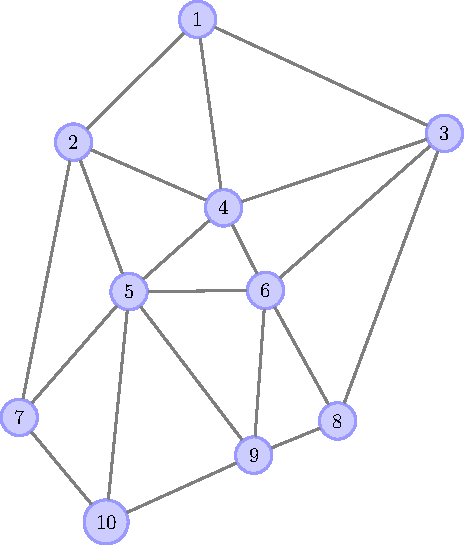
\includegraphics[width=\linewidth]{Figures/graph_plot.pdf}
	\caption[A visual representation of a simple graph]{A visual representation of a simple graph with 10 nodes and 20 edges.}
	\label{fig:basic_graph}
\end{wrapfigure}


Graphs and network models are utilised in many actively researched areas of mathematics, including network processes such as epidemic modelling \citep{Pare2020}, Graph Neural Networks (GNNs) \citep{Zhou2020}, graphical models \citep{Holmes2008}, and semi-supervised learning \citep{Chong2020}.

\vspace{0.1cm}

In this thesis, the subject of focus is Graph Signal Processing (GSP), a rapidly evolving field that sits at the intersection of spectral graph theory, statistics, and data science \citep{Ortega2018}. GSP is an actively researched area devoted to the mathematical analysis of signals that are defined over the nodes of a graph, simply referred to as \textit{graph signals}. \phantom{In this thesis we are  }

\newpage

\begin{wrapfigure}{l}{0.4\linewidth}
	\centering
		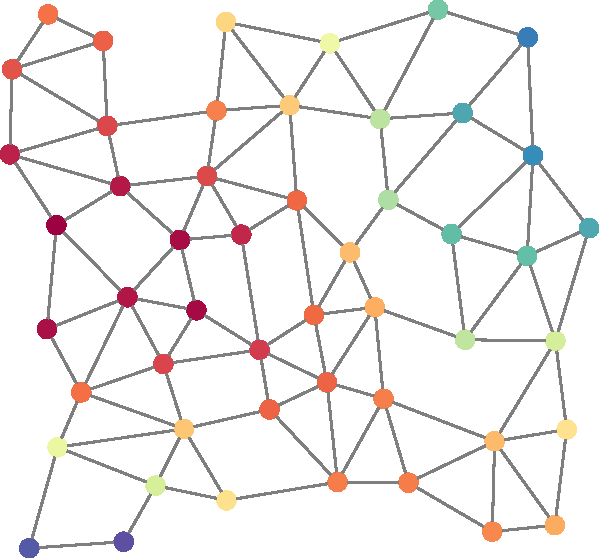
\includegraphics[width=\linewidth]{Figures/graph_signal_plot.pdf}
	\caption[A graphical depiction of a graph signal]{A graphical depiction of a graph signal. Here, the value of the signal at each node is represented by its color.}
	\label{fig:graph_signal}
\end{wrapfigure}
 

A graph signal represents a value that is measured simultaneously at every node in a graph. For example, consider a social media network, where each node represents an individual, and presence of an edge indicates that the two individuals have connected. An example of a graph signal in this context could be the age of each person in the network, or a score indicating their propensity to engage with certain content. In either case, this is a value that could theoretically be measured or estimated across the network, though it may be subject to missing data or noise. 

\vspace{0.2cm}

GSP typically uses tools that stem from classical signal processing, where the goal is to manipulate data that resides on a regular domain such as audio, images or radio. GSP utilises spectral graph theory to generalise these classical techniques, leading to graph-based counterparts of algorithms such as filtering, sampling, and reconstruction \citep{Shuman2013}. Applications of GSP are numerous, ranging from social networks \citep{Dong2015} and brain connectivity modelling \citep{Huang2016} to sensor networks \citep{Zhu2012}, and molecular structures \citep{Kearnes2016}. As an emerging field, there are many opportunities for the development of theory, and new use-cases to explore, making it an exciting and dynamic area of research. 

\section{Research goals}

% multivariate

The goal of this thesis is to provide contributions to the areas of multivariate graph signal reconstruction and regression. A single signal, measured over a network comprising $N$ nodes, is an example of a univariate structure, and can be described by a vector $\y \in \R^N$. Our methods, by contrast, are designed to be applicable to higher-dimensional objects. For example, $T$ samples of a graph signal measured across time can be described by a matrix $\Y \in \R^{N \times T}$. This kind of two-dimensional data can also be viewed as a single graph signal measured on the nodes of a Cartesian product graph \citep{Imrich2000}. More generally, a tensor-valued signal $\Yt \in \R^{N_1 \times N_2 \times ... \times N_d}$ can be understood as a signal on a $d$-dimensional Cartesian product graph \citep{Stanley2020}. 

% GSR + regression

Our aim is to expand the existing literature on multivariate GSP by presenting several novel Bayesian models for reconstructing partially observed graph signals, with and without additional explanatory variables. Graph signal reconstruction is a well-studied topic in GSP, however, the majority of published literature to date has focused on univariate, or time-varying signal models that provide point estimates for the missing values. We aim to generalise this in two ways. First, we present a rich Bayesian formulation, that outputs not only a point estimate, but a full probability distribution quantifying prediction uncertainty. Furthermore, our goal is to produce models applicable to graph signals defined on arbitrary Cartesian product graphs, which naturally extend univariate and time-varying models. While the input to a graph signal reconstruction problem is typically only the partially observed graph signal and the topology of the underlying graph, we also consider the situation in which additional explanatory variables are available to aid in the estimation process. Therefore another key objective of ours is to produce graph signal regression models, applicable to a range of different data scenarios, that are robust to missing data. 

% sampling 

As mentioned, a key aspect of our models is the Bayesian formulation, which produces a full posterior probability distribution over the unknown reconstructed signal, rather than a single point estimate. Given the high-dimensional nature of the data, the posterior covariance, which contains information regarding the corelation between every element in the multivariate signal $\Yt$, is often too large to process with consumer-grade computer hardware. Therefore, another objective of ours is to develop efficient methods for extracting information regarding the prediction uncertainty. In particular, we consider two related but separate tasks: estimating the marginal posterior variance (node-level uncertainty) and drawing samples directly from the posterior. 

% binary

The majority of GSP models tend to focus on real-valued graph signals, leaving signals with binary or categorical entries relatively unexplored. It is therefore an additional goal of ours to develop new statistical reconstruction and regression algorithms for such graph signals. Although related tasks have been examined within semi-supervised learning in machine learning and GNNs in deep learning, we aim to introduce and showcase novel Bayesian models that are grounded firmly in the theoretical framework of GSP.

% complexity 

The high-dimensional nature of the models explore in this thesis comes with a unique set of challenges concerning computational robustness and efficiency. As such, a core objective is to reduce the computational cost of our algorithms wherever possible and to provide a detailed and transparent analysis of their time and memory complexity. The models we present are designed to be applicable to a wide range of application areas, and as such, throughout this thesis we also provide illustrative examples and case-studies to demonstrate their applicability. 

\newpage 


\section{GSP fundamentals}

\label{sec:fundamentals}

A graph, $\mathcal{G}$, with $N$ vertices is described by a node set $\mathcal{V}$, and an edge set $\mathcal{E}$. In this thesis, we will be primarily concerned with undirected graphs without self-loops, meaning the edges have no preferential direction and nodes do not connect to themselves. By imposing some arbitrary but consistent ordering on the nodes, this graph can also be described by an $N \times N$ adjacency matrix $\A$, where the entry $\A_{ij} = \A_{ji} \geq 0$ holds the strength of connection between nodes $i$ and $j$. In the basic case of a non-weighted graph, $\A_{ij}$ is simply one if the corresponding edge exists and zero otherwise. Using the same ordering, a graph signal can be represented by a vector, $\y$, of length $N$, where $\y_i$ holds the value of the graph signal at node $i$. 

One key property of a graph signal is its \textit{smoothness}. Intuitively speaking, a smooth graph signal should exhibit gentle variation between closely connected nodes, as illustrated in \cref{fig:graph_signal}. Conversely, a rough graph signal might see large jumps in signal value between neighbouring nodes. Mathematically, the smoothness of a signal, $\y$, defined over the nodes of an undirected graph, can be measured in several ways. One simple option is the total square variation ($\text{TV}_2$), which is defined as follows. 

\begin{equation}
    \label{eq:TSV1}
    \text{TV}_2(\y) = \frac{1}{2}\sum_{i=1}^N \sum_{j=1}^N \A_{ij} (\y_i - \y_j)^2
\end{equation}

This metric, also known as Dirichlet energy, sums up the square difference in signal value at each neighbouring node, weighted by the corresponding entry in the adjacency matrix, with the factor of a half adjusting for the double counting of nodes. It can also be written in terms of a single quadratic form, by introducing a new matrix $\LL$ - the so-called graph \textit{Laplacian}. 

\begin{equation}
    \label{eq:TSV2}
    \text{TV}_2(\y) = \y^\top \LL \y
\end{equation}

The Laplacian, like the adjacency matrix $\A$, is another symmetric $N \times N$ matrix, and is defined as $\LL = \D - \A$, where $\D$ is the degree matrix. $\D$ is a diagonal operator, where entry $\D_{ii}$ holds the sum of all the edge weights linked to node $i$, or in other words, the vector along the diagonal of $\D$ is the column (or row) sum of $\A$. The Laplacian, which can be interpreted as a generalisation of the discrete second order derivative operator for an irregular topology, is of central importance to many aspects of GSP \citep{Shuman2013}. 

\newpage

It is straightforward to show that the two expressions for the total square variation given in \cref{eq:TSV1,eq:TSV2} are equivalent; see for example chapter 3 of \cite{Ortega2022}. A few basic facts stand out about the Laplacian quadratic form.

\begin{enumerate}
    \item $\y^\top \LL \y \geq 0$ for any $\y$. Since $\text{TV}_2(\y)$ sums the square difference between the signal at each pair of nodes, weighted by the non-negative entries of the adjacency matrix, the Laplacian quadratic form must be strictly non-negative. By definition, this implies that the matrix $\LL$ is positive semi-definite (PSD). 
    \item $\one^\top \LL \one = 0$, where $\one$ is a length-$N$ vector of ones. If the signal of interest is constant over the whole graph, the total square variation must be zero. Moreover, if the graph contains two or more isolated sub-graphs, with edges connecting nodes within a each clique but not between cliques, then any signal that is constant over each sub-graph will have a Laplacian quadratic form of zero. 
\end{enumerate}

Since $\LL$ is positive semi-definite, its eigenvalues are all real and non-negative, and its eigenvectors can be chosen to be real and orthonormal. Thus, $\LL$ can be decomposed as follows. 

\begin{equation}
    \LL = \U \LAM \U^\top
\end{equation}

Here, $\U$ is the orthogonal, $N \times N$ matrix of eigenvectors ${\uu_i}$, and $\LAM$ is the diagonal matrix of corresponding eigenvalues ${\lambda_i}$, typically arranged in ascending order. As $\U$ is orthonormal, it holds that $\uu_i^\top \uu_j = \delta_{ij}$, and that ${\uu_i}$ form a set spanning $\R^N$. Given the definition of the Laplacian quadratic form, the eigenvectors are the unique set of orthonormal vectors that sequentially minimise the total square variation, subject to perpendicularity to all those preceding \citep{Spielman2019}.


$$
\begin{matrix}
    \uu_1 & = & \underset{\raisebox{-0.1cm} { $ \scriptstyle |\uu|^2 = 1$ }}{\text{argmin}} \quad & \text{TV}_2(\uu) \\[0.7cm]
    \uu_2 & = & \underset{\raisebox{-0.1cm} { $ \scriptstyle |\uu|^2 = 1, \; \perp \uu_1$ }}{\text{argmin}} \quad & \text{TV}_2(\uu) \\[0.7cm]
    \uu_3 & = & \underset{\raisebox{-0.1cm} { $ \scriptstyle |\uu|^2 = 1, \;\perp \uu_1, \uu_2$ }}{\text{argmin}} \quad & \text{TV}_2(\uu) \\[0.7cm]
    \uu_4 & = & \ldots
\end{matrix}
$$

\newpage

In this way, the eigenvectors of the graph Laplacian can be understood as sequentially less smooth with respect to the topology of the graph. The corresponding eigenvalue, referred to as the frequency, gives a value specifying how ``rough'' each eigenvector is relative to the others, as measured by $\text{TV}_2$. Note that, for any undirected graph, the first Laplacian eigenvector will always be constant with an eigenvalue of zero. \Cref{fig:uk_eigs} gives a visual depiction of the first eight Laplacian eigenvectors and eigenvalues for a network representing local authority regions in the UK. \footnote{Using boundary data published by the Office for National Statistics \citep{ONS2019}}  

\begin{figure}[t]
	\centering
		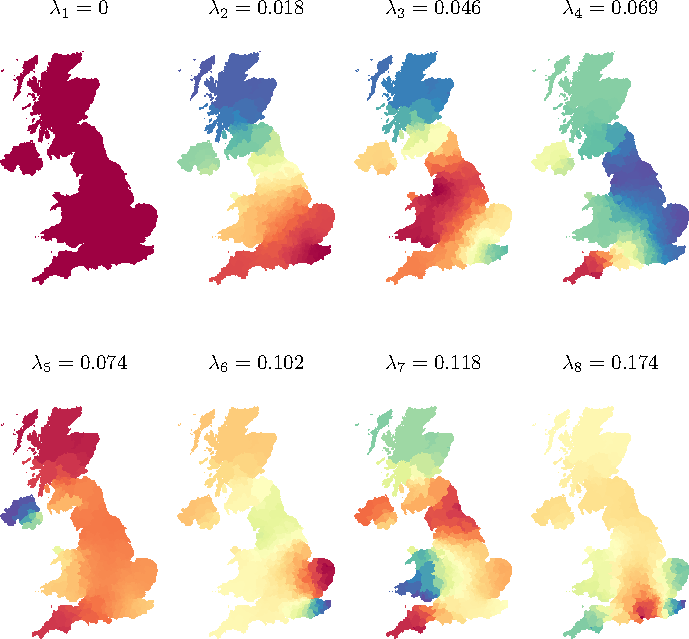
\includegraphics[width=0.85\linewidth]{Figures/uk_plot.pdf}
		% \rule{35em}{0.5pt}
        \caption[A visualisation of the Laplacian eigenvectors for a network of regions in the UK]{A visualisation of the first eight Laplacian eigenvectors, alongside their associated eigenvalues, for a network of local authority regions in the UK. Each node represents a region, and each pair of regions share an edge if they border one another (or have a direct ferry crossing). Colour is used to represent the value of the graph signal.  }
	\label{fig:uk_eigs}
\end{figure}


Since ${\uu_i}$ span the total space of $\R^N$, any graph signal, $\y$, can be decomposed into a weighted sum of the Laplacian eigenvectors. This parallels the classical Fourier transform, which expands signals into the basis of complex exponentials \citep{Sneddon1995}. As such, any graph signal, $\y$, has a dual representation, $\z$, in the frequency domain. Transformations between these two representations can be achieved by applying the Graph Fourier Transform (GFT) and Inverse Graph Fourier Transform (IGFT), which amount to multiplying by the matrices $\U^\top$ and $\U$, respectively.

\begin{align}
    \z &= \mkern 2mu \text{GFT}(\y) \mkern 2mu = \U^\top \y \\[0.2cm]
    \y &= \text{IGFT}(\z)  = \U \z
\end{align}

For some simple graphs, the GFT is equivalent to a well-known transform in classical signal processing. For example, the Laplacian of the cycle graph (i.e. a set of nodes connected in a loop) has eigenvectors that can be expressed as sines and cosines (or, in full generality, complex exponentials) as visualised in \cref{fig:cycle_eighs}. This helps establish a rigorous connection between GSP and classical signal processing, through the study of Algebraic Signal Processing (ASP) \citep{Puschel2003,Sandryhaila2013}. With the GFT and IGFT defined, a wide range of potential models are opened up, many of which can be understood as direct generalisations of methods from conventional signal processing. Classical tasks such as filtering, denoising, reconstruction, sampling, compression etc. can all be translated into the GSP paradigm, setting the stage for a new era of signal processing that leverages graph structures for more complex and rich data analysis, and opening the door to a wealth of novel applications.

\begin{figure}[t]
	\centering
		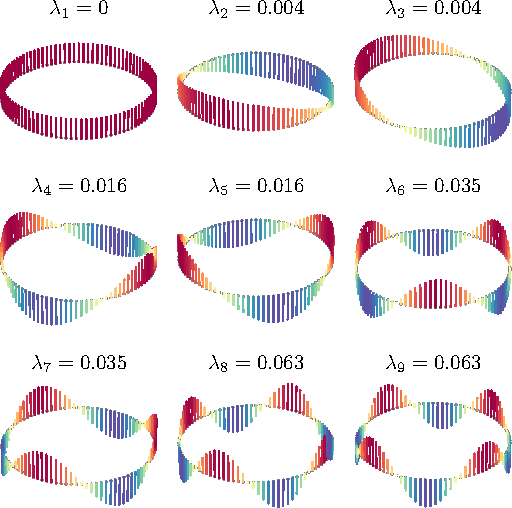
\includegraphics[width=0.65\linewidth]{Figures/loop_plot.pdf}
        \caption[A visualisation of the Laplacian eigenvectors of the cycle graph]{A visualisation of the first nine Laplacian eigenvectors of a cycle graph with 50 nodes, along with their associated eigenvalue.}
	\label{fig:cycle_eighs}
\end{figure}




% Given that any graph signal can be decomposed into its Laplacian frequency components, filters and other spectral operators can be defined quite naturally. First, take a signal $\y$ and transform it into the frequency domain via the GFT. Next, scale each frequency component according to some predetermined function. Finally, transform back into the node domain via the IGFT. 


% \begin{wraptable}{l}{0.5\linewidth}
%     \centering
%     \def\arraystretch{1.7}
%     \begin{tabular}{@{}l c@{}}
%         \toprule
%         \textbf{Filter}   & $g(\lambda; \,\beta)$   \\
%         \midrule
%         1-hop random walk & $(1 + \beta \lambda)^{-1}$ \\
%         Diffusion         & $\exp(-\beta \lambda)$\\
%         ReLu              & $\max (1 - \beta \lambda, 0)$\\
%         Sigmoid           & $2 \big( 1 + \exp(\beta \lambda)\big)^{-1}$\\
%         Bandlimited       & $1, \,\text{if} \; \beta \lambda \leq 1 \; \text{else} \; 0$ \\
%         \bottomrule
%        \end{tabular}
%        \caption[Example graph filter functions]{Some example graph filter functions}
%         \label{tab:filters}
% \end{wraptable}

% A low-pass filter is a spectral operator that attenuates high-frequency components from a graph signal \citep{Ricaud2019}. It can be described by a monotonically decreasing filter function, $g(\lambda)$, which maps a Laplacian frequency, $\lambda$, to a number ranging between one and zero. The filtered signal, $\y'$, can then be computed as follows. 


% \begin{equation}
%     \y' \, =\U \mkern 2mu g(\LAM) \mkern 2mu \U^\top = \, \HH \y
% \end{equation}


% Here, $g(\LAM)$ is the diagonal matrix obtained by applying the function $g(\cdot)$ to each entry along the diagonal of $\LAM$, and $\HH = \U g(\LAM) \U^\top$ is the resultant positive semi-definite graph filter operator \citep{Isufi2022}. \Cref{tab:filters} provides some example filter functions, which also depend on a positive scalar parameter $\beta$ controlling the intensity of the filtering operation. Larger values of $\beta$ correspond to more aggressive attenuation of the high-frequency content. In the limit as $\beta \rightarrow \infty$, these filters retain only the constant component, and as $\beta \rightarrow 0$, all frequency components pass through the filter unaffected.

% Graph filters can also be constructed in other ways. One notable example is using finite order polynomials. The advantage of polynomial filters is that their action on a graph signal can be computed by repeated application of the Laplacian, meaning $O(N^3)$ eigendecomposition can be avoided. An order-$P$ polynomial filter $g(\lambda) = \sum^P a_p \lambda^p$ can be applied to a graph signal as follows \citep{Susnjara2015}. 

% \begin{equation}
%     \U \mkern 2mu g(\LAM) \mkern 2mu \U^\top \y = \big(a_0 \I_N + a_1 \LL + a_2 \LL^2 + ... + a_P \LL^P \mkern 2mu \big) \, \y
% \end{equation}

% If the Laplacian is sparse, or has special structure, repeated multiplications of $\y$ by $\LL$ can computed with complexity $ < O(N^2)$. Furthermore, the computation is ``local'' in the sense that element $i$ of the filtered signal can be computed using data no more than $P$ hops away via graph edges. For this reason, polynomial filters lend themselves well to distributed GSP applications, such as a network of sensors that communicate locally in the vertex domain. \Cref{fig:filters_plot} gives a visualisation of the filter functions given in \cref{tab:filters}, and a polynomial filter. 

% \begin{figure}[t]
% 	\centering
% 		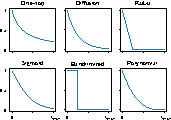
\includegraphics[width=0.7\linewidth]{Figures/filters_plot.pdf}
%         \caption[The frequency response of some simple graphs filters]{The frequency response of several simple graph filters is shown. }
% 	\label{fig:filters_plot}
% \end{figure}


\newpage

\section{Example applications}

Graph signal processing methods have proven effective in many real-world applications. In this short section, we highlight some use-cases from the literature, serving as motivation for the content of this thesis. Many of these areas are utilised within illustrative examples for the methods developed in this thesis. 

\subsection{Biology}

The world of biology provides numerous interesting use cases for graph signal processing methods \citep{Li2023}. One area which has garnered significant interest is in analysing protein-protein interactions. Here, the concept is to model a set of proteins as nodes in an ``interactome'', which is the network of physical molecular interactions in a particular cell. Recent work such as \cite{Colonnese2021} used GSP methods to predict new interactions between proteins, while work such as \cite{Jha2022} used graph neural networks for the same task. These models aim to automate the prediction of protein interactions, reducing the time and cost associated with experimental methods. Other work has modelled an individual protein molecule as network of residues connected to each other based on their physical distance in 3D space, with the aim of predicting its biophysical properties \citep{Srivastava2023}. 

Another domain in biology that has benefited from GSP methods is brain connectivity modelling. Studies such as \cite{Goldsberry2017,Atasoy2016,Menoret2017,Itani2021} have found that the graph-spectral frequency profile of signals derived from fMRI imaging can provide valuable insight into brain activity. Specifically, these and related works have identified specific Laplacian spectral profiles associated with different emotional states, task familiarity, and neurological diseases.

\subsection{Transportation and infrastructure}

Another domain in which GSP methods have been extensively applied is transportation and infrastructure. In \cite{Hasanzadeh2017}, the authors propose an adaptive ARMA model in the graph frequency domain for real-time traffic prediction, achieving a substantial performance increase over non-graph-aware alternatives. Traffic prediction was also addressed using GSP methods in \cite{Chakraborty2017} with a technique known as trend filtering \citep{Wang2016}. Automatic incident detection using spatio-temporally denoised thresholds was applied in \citep{Chakraborty2019}. In \cite{Xiu2022}, the authors used a spatial-temporal multi-graph convolutional wavelet network to predict passenger numbers on a metro system.

GSP has also been employed to analyse patterns of power consumption in electricity grids \citep{Ramakrishna2021} and pressure in hydraulic networks \citep{Zhou2022}. In \cite{He2018} and \cite{Zheng2022}, the authors utilised GSP to address non-intrusive load disaggregation—an active area of research in the field of smart grids and energy conservation where the goal is to estimate each appliance's contribution to total consumption. In \cite{Ying2022}, the authors tackle the recovery of harmonic data lost during power transmission, based on spectral graph theory, and in \cite{Wang2022b}, the authors use GSP to identify abnormal batteries from cell-level voltage signals in a network of electric bicycle charging stations.


\subsection{Finance and economics}

Networks have been used in financial and economic models for many years \citep{Marti2021}, yet recently GSP has found some interesting use-cases. In \cite{Vinicius2020}, the authors employ a spectral model to learn an underlying graph structure from financial time-series data, showing that meaningful physical interpretations related to the market index factor can be extracted from this representation. In \citep{Zhang2023}, the authors consider how GSP can be incorporated into momentum-based financial forecasting models, demonstrating that the additional topological information can enhance the accuracy of such models.

GSP has also been used recently in the context of asset allocation and portfolio theory. The portfolio cut paradigm, introduced in \citep{Dees2020}, is a graph-theoretic portfolio partitioning technique that enables investors to group economically meaningful clusters of assets. In \citep{Arroyo2022}, this concept is extended to include a dynamic portfolio, with time-evolving clusters.

Graph Neural Networks have also been used extensively in financial applications \citep{Wang2022c}. 


\subsection{Sensor networks}

Sensor networks are a classic application for GSP methods, as a graph is typically straightforward to construct from the physical positioning of the devices \citep{Jablonski2017}. Many applications in this domain focus on distributed algorithms, as sensors and IoT devices are naturally suited to local communication. The aims of such applications are varied, encompassing tasks like compression \citep{Zhu2012}, denoising \citep{Tay2021}, reconstruction \citep{Wang2015}, and distributed data processing \citep{Chi2022}.

Some of the earliest work classified as GSP involved applications with sensor data, for example, \cite{Guestrin2004}. Here, the authors used local basis functions to design a regression algorithm capable of fast convergence with only local communication. In \cite{Wagner2005}, the authors develop a distributed wavelet transform and applied it to a signal compression task over a network of sensors. 

\section{Thesis organisation}

The core content of this thesis begins in \cref{chap:gsr_2d}, with the reconstruction of signals with two axes, such as network time series data. \Cref{chap:kgr_rnc_2d} introduces several regression techniques for two-dimensional graph signals, and \cref{chap:nd_gsp} generalises the techniques developed prior in the thesis to $d$-dimensional data, under the ``MultiWay" GSP (MWGSP) framework. This is followed, in \cref{chap:variance}, by an investigation into the posterior covariance of the models, and finally \cref{chap:binary} introduces generalisations for binary and categorical graph signals. Along the way, there are several methodological contributions as well as some detailed case studies. In \cref{chap:lit_review}, we define the precise scope of this thesis, review the relevant literature, and present our core contributions. 


\chapter{Literature Review and Contributions} % Main chapter title

\label{chap:lit_review} % Change X to a consecutive number; for referencing this chapter elsewhere, use \ref{ChapterX}

\lhead{Chapter 2. \emph{Literature Review and Contributions}} % Change X to a consecutive number; this is for the header on each page - perhaps a shortened title


\section{Graph Signal Processing}


\subsection{A broad overview of the field}

\subsection{Applications}

Biological: 

Sensors: \cite{Jablonski2017}


\subsection{The graph Laplacian}

\cite{LeMagoarou2016}


\subsection{Graph filters}

\subsubsection{Graph Kernels}

\cite{Kondor2002}

\cite{Smola2003}

\cite{Zhu2003}

\cite{Zhi2023}


\begin{table}[b]
    \renewcommand{\arraystretch}{1.7}
    \small
    \begin{center}
    \begin{tabular}{|l|c|}
    \hline
    \textbf{Filter}   & $g(\lambda; \,\beta)$    \\ 
    \hline
    1-hop random walk & $(1 + \beta \lambda)^{-1}$ \\
    \hline
    Diffusion         & $\exp(-\beta \lambda)$       \\
    \hline
    ReLu              & $\max (1 - \beta \lambda, 0)$  \\
    \hline
    Sigmoid           & $2 \big( 1 + \exp(\beta \lambda)\big)^{-1}$ \\
    \hline
    Bandlimited       & $1, \,\text{if} \; \beta \lambda \leq 1 \; \text{else} \; 0$   \\
    \hline
    \end{tabular}
    \end{center}
    \caption{Isotropic graph filter functions}
    \label{tab:iso_filters}
    \end{table}



\section{Regression and Reconstruction}

\cite{Guestrin2004} Regression


\subsection{Graph Signal Reconstruction}

\cite{Qiu2017} Time varying signal reconstruction. 

\subsection{Kernel Graph Regression}

\cite{Takeda2007}

\cite{Elias2022}

\cite{Venkitaraman2019}


\subsubsection{Gaussian Processes on Graphs}

\cite{Venkitaraman2020}

\cite{Miao2022}: GPoG + graph learning

\subsection{Regression with Network Cohesion}

\cite{Le2022}

\cite{Li2019}

\section{GSP on higher order graphs}

Multiway data processing 

\cite{Smilde2004}
\cite{Kroonenberg2008}


\cite{Ji2019}

\cite{Cammoun2009}




\subsection{Multi-Layer Graph Signal Processing}

\cite{Zhang2022} describe M-GSP 

\cite{Zhang2018} extend M-GSP to multiple layers with different number of nodes by adding fake nodes in where they are missing from layers. 
 

\subsection{Multi-Way Graph Signal Processing}


\cite{Zhao2023}

\cite{Li2012}



\section{classification}

\cite{Tran2020}

No one has done it on multiway graphs. Limited regression models. No one using graph filters. 


\section{What it's not}

Directed graphs  \cite{Chung2005, Bauer2012}

Total variation: \citep{Shafipour2019,Sardellitti2017}

Magnetic Laplacian \citep{DeResende2020,Zhang2021,Furutani2020}

Graph neural networks, distributed, graph learning

\chapter{Signal Reconstruction on Cartesian Product Graphs}

\label{chap:gsr_2d}

\lhead{Chapter 3. \emph{Regression and Reconstruction on Cartesian Product Graphs}}

% What are we doing? 

In this chapter, we address the topic of signal reconstruction over general two-dimensional Cartesian product graphs, where an arbitrary set of signal elements is missing. The first key objective is to present a novel Bayesian model for this purpose, based on our formulation of multivariate graph filters, where a smooth underlying signal must be inferred given a noisy partial observation. The second is to produce two scalable iterative algorithms for computing the posterior mean and investigate their respective convergence properties both theoretically and empirically. 

% why is this useful?

As discussed in \cref{sec:GSR_review}, Graph Signal Reconstruction (GSR) is a topic that has received substantial attention in the last decade. Whilst the majority of past models have focused on the reconstruction of a single one-dimensional signal, with some recent models extending this to time-varying signals, our approach can be seen as a natural generalisation that encompasses two-dimensional matrix signals with arbitrary undirected graphs underlying each axis. Furthermore, we believe our Bayesian approach can offer new insight into multivariate correlation structure over irregular topologies. Since efficient computation is a critical factor in real-world applications of GSR, we devote substantial attention to a careful analysis of computational complexity. In doing so, we show how the two iterative algorithms we present possess different convergence behaviour and implementation details, making the optimal choice dependent on the hyperparameters, data composition, and graph sparsity. 


% chapter layout

We begin in \cref{sec:reg_and_rec_intro} by reviewing the concept of a graph product, explaining our rationale for focusing on the Cartesian product in particular, and introducing our model for two-dimensional anisotropic filters. In \cref{sec:gsr_cpg}, we present our statistical model for graph signal reconstruction on a Cartesian product graph and derive the two algorithms for solving the posterior mean. These encompass a Stationary Iterative Method (SIM) based on matrix splitting and a Conjugate Gradient Method (CGM) using a graph-spectral preconditioner. In addition, we show how the SIM can be implemented using Chebyshev polynomials to avoid Laplacian eigendecomposition. To end this section, we demonstrate the utility of these models using a dataset comprising daily SARS-CoV-19 case rates across the UK. Finally, in \cref{sec:convergence}, we engage in an in-depth analysis of the convergence properties of each method and propose practical guidelines for method selection. 


\section{Graph Products}

\label{sec:reg_and_rec_intro}

In this chapter, we will be primarily concerned with signal processing on \textit{Cartesian product graphs}. This special class of graph finds applications in numerous areas, such as video, hyper-spectral image processing and network time series problems. However, the Cartesian product is not the only way to consistently define a product between two graphs. In this section, we formally introduce the concept of a graph product, examine several prominent examples, and explain why we choose to look specifically at the Cartesian graph product.

\subsection{Basic definitions}

\label{sec:graph_products_defined}

In the general case, consider two undirected graphs $\mathcal{G}_A = (\mathcal{V}_A, \mathcal{E}_A)$ and $\mathcal{G}_B = (\mathcal{V}_B, \mathcal{E}_B)$ with vertex sets given by $\mathcal{V}_A = \{a \in \mathbb{N} \, | \, a \leq N_A \}$ and $\mathcal{V}_B = \{b \in \mathbb{N} \, | \, b \leq N_B \}$ respectively. (In this context we do not regard zero to be an element of the natural numbers, with node indices beginning from zero). A new graph $\mathcal{G}$ can be constructed by taking the product between $\mathcal{G}_A$ and $\mathcal{G}_B$. In its most general form, this can be written as follows.

\begin{equation}
    \mathcal{G} = \mathcal{G}_A \, \diamond \, \mathcal{G}_B = (\mathcal{V}, \, \mathcal{E})
\end{equation}

For all common definitions of a graph product $\diamond$, the resultant graph $\mathcal{G}$ has a vertex set $\mathcal{V}$ given by the Cartesian product of the vertex sets of the corresponding factor graphs, that is

\begin{equation}
    \mathcal{V} = \mathcal{V}_A \times \mathcal{V}_B = \{(a, \, b) \in \mathbb{N}^2 \, | \, a \leq N_A \; \text{and} \; b \leq N_B \}
\end{equation}

Typically, vertices are arranged in lexicographic order, in the sense that $(a, \, b) \leq (a',\, b')$ iff $a < a'$ or ($a = a'$ and $b \leq b'$) \citep{Harzheim2005}. To define a product, one must specify a consistent rule for constructing the new edge set $\mathcal{E}$ from the factor edge sets $\mathcal{E}_A$ and $\mathcal{E}_B$. In general, there are eight possible conditions for deciding whether two nodes $(a, \, b)$ and $(a',\,  b')$ are to be connected in the new graph.


\begin{table}[h]
    \def\arraystretch{1.5}
    \centering
    \begin{tabular}{lclc}
        1. & $[a, \, a'] \in \mathcal{E}_A$    & and & $b = b'$                          \\
        2. & $[a, \, a'] \notin \mathcal{E}_A$ & and & $b = b'$                          \\
        3. & $[a, \, a'] \in \mathcal{E}_A$    & and & $[b, \, b'] \in \mathcal{E}_B$    \\
        4. & $[a, \, a'] \notin \mathcal{E}_A$ & and & $[b, \, b'] \in \mathcal{E}_B$    \\
        5. & $[a, \, a'] \in \mathcal{E}_A$    & and & $[b, \, b'] \notin \mathcal{E}_B$ \\
        6. & $[a, \, a'] \notin \mathcal{E}_A$ & and & $[b, \, b'] \notin \mathcal{E}_B$ \\
        7. & $a = a'$                          & and & $[b, \, b'] \in \mathcal{E}_B$,   \\
        8. & $a = a'$                          & and & $[b, \, b'] \notin \mathcal{E}_B$
    \end{tabular}
\end{table}



Each definition of a graph product corresponds to the union of a specific subset of these conditions, thus, there exist 256 different types of graph product \citep{Barik2015}. Of these, the Cartesian product (conditions 1 or 7), the direct product (condition 3), the strong product (conditions 1, 3 or 7) and the lexicographic product (conditions 1, 3, 5 or 7) are referred to as the standard products and are well-studied \citep{Imrich2000}. A graphical depiction of the standard graph products is shown in figure \ref{fig:graph_products}. In each of these four cases, the adjacency and Laplacian matrices of the product graph can be described in terms of matrices relating to the factor graphs \citep{Fiedler1973, Barik2018}. This is shown in table \ref{tab:grap_product_matrices}.

\begin{table}[b]
    \def\arraystretch{1.9}
    \centering
    \small
    \vspace{0.5cm}
    \setlength{\tabcolsep}{10pt}
    \begin{tabular}{l c c}
        \toprule

         & Adjacency matrix & Laplacian \\

        \midrule

        Cartesian
         & $\A_A \oplus \A_B$
         & $\LL_A \oplus \LL_B$                                                                   \\

        Direct
         & $\A_A \otimes \A_B$
         & $\D_A \otimes \LL_B + \LL_A \otimes \D_B - \LL_A \otimes \LL_B$                        \\

        Strong
         & $\A_A \otimes \A_B + \A_A \oplus \A_B$
         & $\D_A \otimes \LL_B + \LL_A \otimes \D_B - \LL_A \otimes \LL_B + \LL_A \oplus \LL_B$   \\

        Lexicographic
         & $\I_A \otimes \A_B + \A_A \otimes \OO_A$
         & $\I_A \otimes \LL_B + \LL_A \otimes \OO_B + \D_A \otimes (N_B \I_B - \OO_B)$ \\

        \bottomrule
    \end{tabular}
    \vspace{0.2cm}
    \caption[The adjacency and Laplacian matrices for the standard graph products]{The adjacency and Laplacian matrices for the standard graph products. Here, $\D_A$ and $\D_B$ are the diagonal degree matrices, i.e $\D_A = \diag{\A_A \mathbf{1}}$. $\I_A$ and $\OO_A$ are the $(N_A \times N_A)$ identity matrix and matrix of ones respectively. }
    \vspace{0.3cm}
    \label{tab:grap_product_matrices}
\end{table}



\begin{figure}[t]
    \begin{center}
        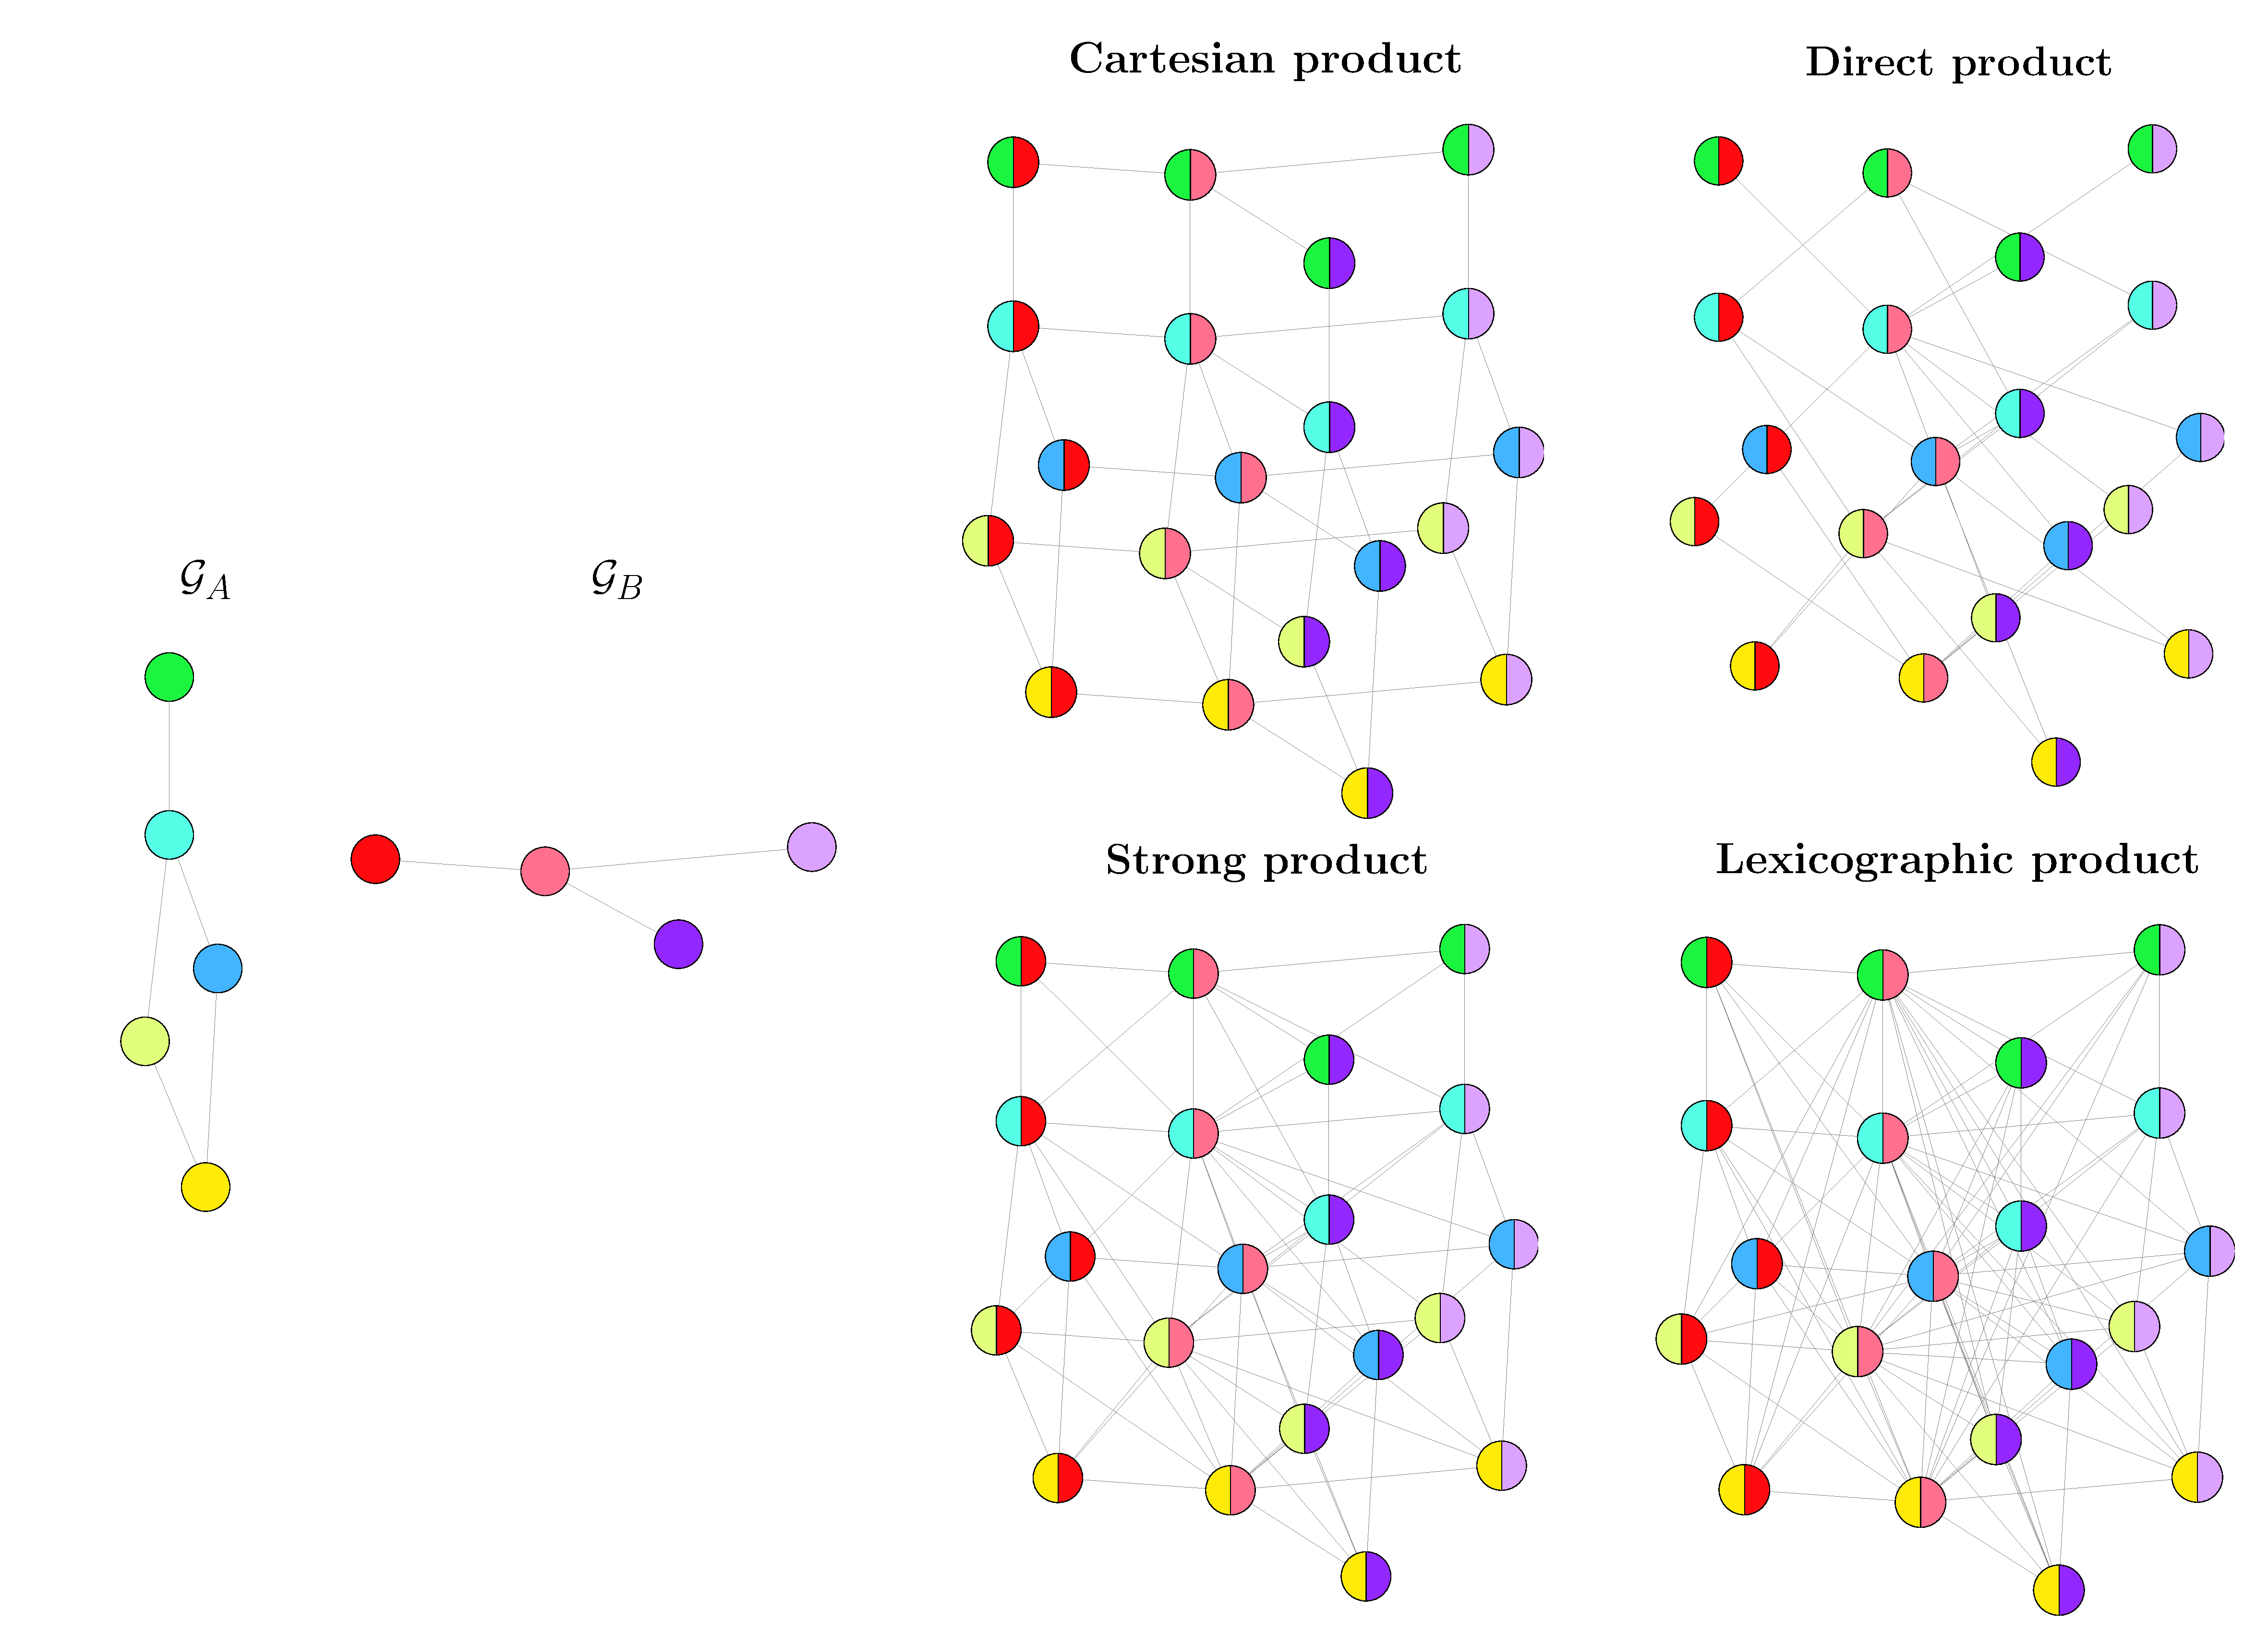
\includegraphics[width=0.95\linewidth]{Figures/product_graphs.pdf}
    \end{center}
    \caption[Graphical depiction of the standard graph products]{A graphical depiction of the four standard graph products}
    \label{fig:graph_products}
\end{figure}

Given these definitions, it may seem that all the standard graph products are non-commutative in the sense that $\A_A \oplus \A_B  \neq \A_B \oplus \A_A $ etc. However, the graphs $\mathcal{G}_A \, \diamond \, \mathcal{G}_B$ and $\mathcal{G}_B \, \diamond \, \mathcal{G}_A$ are in fact isomorphically identical in the case of the Cartesian, direct and strong products. This is not the case for the Lexicographic product \citep{Imrich2000}.

\subsection{The spectral properties of products graphs}

In the field of graph signal processing, we are often concerned with analysing the properties of graphs via eigendecomposition of the graph Laplacian \citep{Mieghem2010}. In the case of product graphs, it is greatly preferable if we can fully describe the spectrum of $\mathcal{G}_A \diamond \mathcal{G}_B$ in terms of the spectra of $\mathcal{G}_A$ and $\mathcal{G}_B$ alone. This is because the direct decomposition of a dense $\LL$ has time-complexity $O(N_A^3N_B^3)$, whereas decomposition of the factor Laplacians individually has complexity $O(N_A^3 + N_B^3)$. As the graphs under consideration become medium to large, this fact quickly makes direct decomposition of the product graph Laplacian intractable. However, in the general case, only the spectra of the Cartesian and lexicographic graph products can be described in this way \citep{Barik2018}. In the case of the direct and strong product, it is possible to estimate the spectra without performing the full decomposition (see \citep{Sayama2016}). However, in general, the full eigendecomposition of the product graph Laplacian can only be described in terms of the factor eigendecompositions when both factor graphs are regular.


Consider the eigendecompositions of $\LL_A$ and $\LL_B$.

\begin{equation}
    \LL_A = \U_A \LAM_A \U_A^\top, \aand \LL_B = \U_B \LAM_B \U_B^\top
\end{equation}

where $\U_A$ and $\U_B$ are the respective orthonormal eigenvector matrices, and $\LAM_A$ and $\LAM_B$ are the diagonal eigenvalue matrices given by

\begin{equation*}
    \LAM_A = \diag{\begin{bmatrix} \lambda_1^{(A)}, & \lambda_2^{(A)}, & \dots & \lambda_A^{(A)} \end{bmatrix}},
    \aand
    \LAM_B = \diag{\begin{bmatrix} \lambda_1^{(B)}, & \lambda_2^{(B)}, & \dots & \lambda_B^{(B)} \end{bmatrix}}
\end{equation*}

Given these definitions, table \ref{tab:product_graph_spectra} gives information about the spectral decomposition of the standard graph products.

\begin{table}[t]
    \def\arraystretch{2}
    \centering
    \small
    \vspace{0.5cm}
    \begin{tabular}{l c c}
        \toprule

         & Eigenvalues
         & Eigenvectors                                                                          \\

        \midrule

        Cartesian
         & $\lambda_a^{(A)} + \lambda_b^{(B)}$
         & $(\U_A)_a \otimes (\U_B)_b$                                                           \\

        Direct$^{\star}$
         & $r_A \lambda_b^{(B)} + r_B \lambda_a^{(A)} - \lambda_a^{(A)} \lambda_b^{(B)}$
         & $(\U_A)_a \otimes (\U_B)_b$                                                           \\

        Strong$^{\star}$
         & $(1+r_A) \lambda_b^{(B)} + (1+r_B) \lambda_a ^{(A)}- \lambda_a^{(A)} \lambda_b^{(B)}$
         & $(\U_A)_a \otimes (\U_B)_b$                                                           \\

        \multirow{2}{7em}{Lexicographic$^\dagger$}
         & $N_B \lambda_a^{(A)}$
         & $(\U_A)_a \otimes \mathbf{1}_B$                                                       \\

         & $\lambda_b^{(B)} + N_B \text{deg}(a)$
         & $\mathbf{e}_a \otimes (\U_B)_b$                                                       \\

        \bottomrule
    \end{tabular}
    \vspace{0.2cm}
    \caption[Spectral decomposition of product graphs]{Eigendecomposition of the Laplacian of the standard graph products. Here, $a$ and $b$ are understood to run from 1 to $N_A$ and 1 to $N_B$ respectively. $\star$ only for $r_A$ and $r_B$-regular factor graphs. $\dagger$ note that the $b$ runs from 2 to $N_B$ in the lower row. }
    \vspace{0.3cm}
    \label{tab:product_graph_spectra}
\end{table}

% remark common degree locally only necessary 
% subspace concentration 


\subsection{Signals and filters on Cartesian product graphs}

\label{sec:gsp_cpg}

While both the direct and strong products do find uses in certain applications (for example, see \citep{Kaveh2011}), they are both less common and more challenging to work with in a graph signal processing context due to their spectral properties described in the previous subsection. In practice, being limited to regular factor graphs means the majority of practical GSP applications are ruled out. The lexicographic product does not share this drawback, however, it is also significantly less common than the Cartesian product in real-world applications. For this reason, in the following, we focus primarily on the Cartesian product.

Given the spectral decomposition of the Cartesian graph product stated in table \ref{tab:product_graph_spectra}, we can write the Laplacian eigendecomposition in matrix form as follows.

\begin{equation}
    \LL = \U \LAM \U^\top, \where \U = \U_A \otimes \U_B \aand \LAM = \LAM_A \oplus \LAM_B
\end{equation}

This motivates the following definitions for the Graph Fourier Transform (GFT) and its inverse (IGFT). Consider a signal defined over the nodes of a Cartesian product graph expressed as a matrix $\Y \in \R^{N_B \times N_A}$. We can perform the GFT as follows.


\begin{equation}
    \label{eq:GFT_2d}
    \text{GFT}(\Y) = \mat{\big( \U_A^\top \otimes \U_B^\top \big) \, \vecc{\Y}} = \U_B^\top \Y \U_A
\end{equation}

Correspondingly, we can define the IGFT acting on a matrix of spectral components $\Z \in \R^{N_B \times N_A}$ as follows.

\begin{equation}
    \label{eq:IGFT_2d}
    \text{IGFT}(\Z) = \mat{\big( \U_A \otimes \U_B \big)\,\vecc{\Z}} = \U_B \Z \U_A^\top
\end{equation}


\note{Product graph signals: representation and vectorisation}{

    It is natural to assume that signals defined on the nodes of a Cartesian product graph $\mathcal{G}_A \, \square \; \mathcal{G}_B$ could be represented by matrices (order two tensors) of shape $(N_A \times N_B)$. Since product graph operators, such as the Laplacian $\LL_A \oplus \LL_B$, act on vectors of length $N_A N_B$, we must define a consistent function to map matrix graph signals $\in \R^{N_A \times N_B}$ to vector graph signals $\in \R^{N_A N_B}$. The standard mathematical operator for this purpose is the $\vecc{\cdot}$ function, along with its reverse operator $\mat{\cdot}$. However, this is somewhat problematic since $\vecc{\cdot}$ is defined to act in \textit{column-major} order, that is

    $$
        \text{vec} \left( \begin{bmatrix}
                \Y_{(1, 1)} & \Y_{(1, 2)} & \dots  & \Y_{(1, N_B)} \\
                \Y_{(2, 1)} & \Y_{(2, 2)} & \dots  & \Y_{(2, N_B)} \\
                \vdots      & \vdots      & \ddots & \vdots      \\
                \Y_{(N_A, 1)} & \Y_{(N_A, 2)} & \dots  & \Y_{(N_A, N_B)} \\
            \end{bmatrix} \right)
        =
        \begin{bmatrix}
            \Y_{(1, 1)} \\ \Y_{(2, 1)} \\ \vdots \\ \Y_{(N_A-1, N_B)} \\ \Y_{(N_A, N_B)}
        \end{bmatrix}
    $$

    As is visible, this does not result in a lexicographic ordering of the matrix elements when the graph signal has shape $(N_A \times N_B)$. Therefore, to avoid this issue and to be consistent with standard mathematical notation, we will assume that graph signals are represented by matrices of shape $(N_B \times N_A)$ when considering the product between two graphs $\mathcal{G}_A \, \square \, \mathcal{G}_B$. For graph signals of this shape, the first index represents traversal of the nodes in $\mathcal{G}_B$, and the second index represents traversal of the nodes in $\mathcal{G}_A$. This ensures that matrix elements are correctly mapped to vector elements when using the column-major $\vecc{\cdot}$ function.

}

Given these definitions, we can define a spectral operator (usually a low-pass filter) $\HH$ which acts on graph signals according to a spectral scaling function $g(\lambda \,; \, \beta)$ such as one of those defined in table \ref{tab:iso_filters}. As with regular non-product graphs, the action of this operator can be understood as first transforming a signal into the Laplacian frequency domain via the GFT, then scaling the spectral components according to some function, and finally transforming back into the vertex domain via the IGFT.

\begin{align}
    \label{eq:graph_filter}
    \HH & = g(\LL_A \oplus \LL_B) \notag                                                                                          \\
        & = \big( \U_A \otimes \U_B \big) \, g \big( \LAM_A \oplus \LAM_B \big) \, \big( \U_A^\top \otimes \U_B^\top \big) \notag \\
        & = \big( \U_A \otimes \U_B \big) \, \diag{\vecc{\G}} \, \big( \U_A^\top \otimes \U_B^\top \big) \notag \\
        &= \U \D_\G \U^\top
\end{align}

% remark which section of the thesis the properties of G are explained

The matrix $\G \in \R^{N_B \times N_A}$, which we refer to as the spectral scaling matrix, holds the value of the scaling function applied to the sum of
pairs of eigenvalues, such that

\begin{equation}
    \label{eq:Gba}
    \G_{ba} = g\left(\lambda^{(A)}_a + \lambda^{(B)}_b; \beta\right)
\end{equation}


% remark about Cartesian product eig sum

We observe that defining the filtering operation in this manner implies that the intensity is equal across both $\mathcal{G}_A$ and $\mathcal{G}_B$. We refer to filters of this type as \textit{isotropic}. This can be further generalised by considering an \textit{anisotropic} graph filter, which offers independent control over the filter intensity in each of the two dimensions. In this case, we define $\G$ as follows.

\begin{equation}
    \label{eq:Gba2}
    \G_{ba} =  g \left(\lambda^{(A)}_a, \lambda^{(B)}_b; \, \beta_a, \beta_b\right)
\end{equation}

where now $g$ is chosen to be an anisotropic graph filter such as one of those listed in table \ref{tab:anis_filters_2d}. Note that the original parameter $\beta$ is now replaced by two parameters $\beta_a$ and $\beta_a$ which offer independent control over the filter intensity in each dimension. In order for the definition of a 2D anisotropic filter to remain consistent with the underlying Cartesian product graph, we note that all filters we list are given by a function of a weighted sum of each Laplacian eigenvalue. Other more general functions of $\lambda^{(A)}_a$ and $\lambda^{(B)}_b$ will also result in operators that commute with the Laplacian but cannot be consistently considered graph spectral operators on the Cartesian product graph. 

Similarly defined two-dimensional filters have appeared in image processing literature \citep{Aubert2006}, however, their use in graph signal processing so far has been limited to time-varying graph signal models. In \cite{Romero2017}, the authors propose `space-time kernels', and in \cite{Grassi2018, Isufi2017, Loukas2016, Jiang2021}, the authors discuss joint time-vertex filters. These models can essentially be understood as operating on a two-dimensional Cartesian product graph when one of the graphs takes the form of a path or a cycle graph, which gives rise to the standard Discrete Fourier Transform (DFT) in the time dimension. However, to the best of our knowledge, no one has addressed filters applicable to general two-dimensional Cartesian product graphs. \Cref{fig:filters} depicts an anisotropic graph filter applied to a Cartesian product graph constructed from a 4-node line graph and a generic 10-node. 


\begin{table}[t]
    \vspace*{1cm}
    \def\arraystretch{1.8}
    \begin{center}
        \begin{tabular}{lc}
        \toprule
        \textbf{Filter}   & $g(\lambda_a, \lambda_b; \,\beta_a, \beta_b)$  \\
        \midrule
        1-hop random walk & $(1 + \beta_a \lambda_a + \beta_b \lambda_b)^{-1}$\\
        Diffusion         & $\exp(-\beta_a \lambda_a - \beta_b \lambda_b)$\\
        ReLu              & $\max (1 - \beta_a \lambda_a - \beta_b \lambda_b, 0)$ \\
        Sigmoid           & $2 \big( 1 + \exp(\beta_a \lambda_a + \beta_b \lambda_b)\big)^{-1}$\\
        Gaussian          & $\exp \big(-(\beta_a \lambda_a + \beta_b \lambda_b)^2\big)$\\
        Bandlimited       & $1, \,\text{if} \; \beta_a \lambda_a + \beta_b \lambda_b\leq 1 \; \text{else} \; 0$ \\
        \bottomrule
        \end{tabular}
    \end{center}
    \caption{Anisotropic graph filter functions in two dimensions}
    \label{tab:anis_filters_2d}
    \vspace*{1cm}
\end{table}






\section{Graph Signal Reconstruction on Cartesian Product Graphs}

\label{sec:gsr_cpg}

We now turn our attention to the task of signal reconstruction on Cartesian product graphs. In the following, we will replace the factor graph labels $A$ and $B$ with $T$ and $N$ respectively. The reason for this is that one application of particular interest is graph time-series problems, where we seek to model a network of $N$ nodes across a series of $T$ discrete time points. These so-called ``time-vertex'' (T-V) problems have garnered significant interest recently in the context of GSP \citep{Grassi2018, Isufi2017, Loukas2016}. T-V signals can be understood as existing on the nodes of a Cartesian product graph $\mathcal{G}_T \, \square \, \mathcal{G}_N$. In particular, we can conceptualise $T$ repeated measurements of a signal defined across the nodes of a $N$-node graph as a single measurement of a signal defined on the nodes of $\mathcal{G}_T \, \square \, \mathcal{G}_N$, where $\mathcal{G}_T$ is a simple path graph. In the following subsection, we begin the main contributions of this chapter. 



\clearpage

\vspace*{\fill}

\begin{figure}[h]
    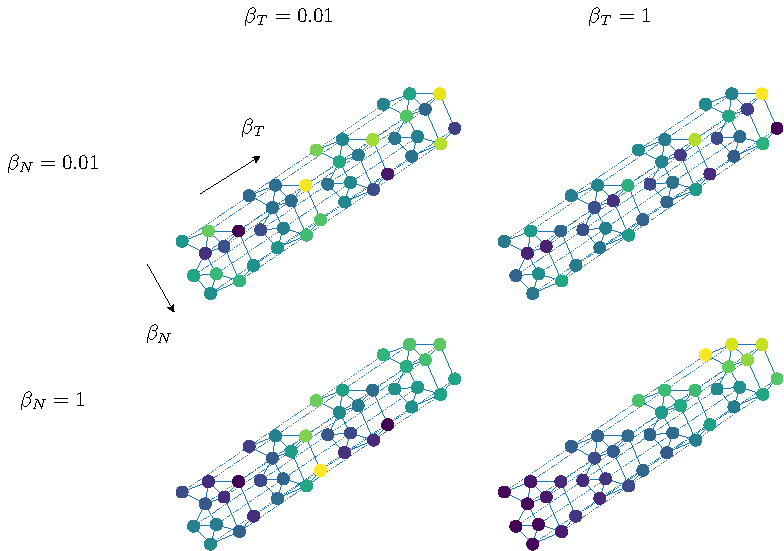
\includegraphics[width=0.95\linewidth]{Figures/2dFilters.pdf}
    \vspace*{1cm}
    \caption[A visual representation of applying an isotropic and anisotropic graph filter]{A visual representation of an anisotropic filter applied to a signal on a Cartesian product graph. In the top left, the filter intensity is low in both dimensions resulting in a signal with no particular correlation. In the top right, the filter intensity is strong in the $T$ dimension, resulting in a longitudinally smoother signal with little cross-sectional correlation. In the lower left, the filter is strong in the $N$ dimension, resulting in smooth cross-sections with little correlation longitudinally. In the lower right, the filter is strong in both dimensions, resulting in a signal that is smooth both cross-sectionally and longitudinally. }
    \label{fig:filters}
\end{figure}

\vspace*{\fill}


\clearpage

\topskip0pt
\vspace*{\fill}
\note{On the Laplacian spectrum of the path graph}{
    \label{box}
    When considering time-vertex problems with uniformly spaced time intervals, $\mathcal{G}_T$ will be described by a path graph with equal weights on each edge. This special case of a graph has vertices given by $\mathcal{V}_T = \{t \in \mathbb{N} \, | \, t \leq T \}$ and edges given by $\mathcal{E}_T = \{ \, [t, t+1] \, | \, t < T \}$. The Laplacian matrix of the path graph is therefore given by

    $$
        \LL_T = \begin{bmatrix}
            1  & -1 &        &    &    \\
            -1 & 2  & -1     &    &    \\
               &    & \ddots &    &    \\
               &    & -1     & 2  & -1 \\
               &    &        & -1 & 1  \\
        \end{bmatrix}
    $$

    The eigenvalues and eigenvectors of this Laplacian are well-known and can be expressed in closed-form \citep{Jiang2012}. In particular,

    $$
        \lambda^{(T)}_t = 2 - 2 \cos \Big(  \, \frac{t - 1}{T} \pi \, \Big)
    $$

    and

    $$
        (\U_T)_{ij} = \cos \Big( \, \frac{j - 1}{T}\big(i - \frac{1}{2}\big)\pi \, \Big)
    $$

    where the columns of $\U$ are appropriately normalised such that the magnitude of each eigenvector is one. Furthermore, this implies that the graph Fourier transform of a signal $\y \in \R^{T}$ is given by the orthogonal type-II Discrete Cosine Transform (DCT) \citep{Ahmed1974}. This is of significance, as it means we can leverage Fast Cosine Transform (FCT) algorithms \citep{Makhoul1980} which operate in a similar manner to the well-known Fast Fourier Transform (FFT) \citep{Cooley1965}. See chapter 4 of \cite{Rao1990} for an overview of FCT algorithms. In general, FFT-type algorithms are challenging to derive for the GFT \citep{LeMagoarou2016}, however, this is a simple case where it can be achieved. 

    \vspace{0.2cm}

    In particular, this reduces both of the following procedures

    \begin{equation*}
        \text{GFT}(\y) = \U_T^\top \y \aand \text{IGFT}(\y) = \U_T \y
    \end{equation*}

    from $O(T^2)$ operations to $O(T \log T)$ operations, which can be significant for large time-series problems. 
}

\vspace*{\fill}



% Note that, despite the observation that $\mathcal{G}_T$ is often a path graph in the context of T-V problems, the methods introduced in this section are valid for the Cartesian product between arbitrary undirected factor graphs.

\newpage 

\subsection{Problem statement}

\label{sec:problem_statement_2d}

\addtolength{\skip\footins}{2pc plus 2pt}

The goal of Graph Signal Reconstruction (GSR) is to estimate the value of a partially observed graph signal at nodes where no data was collected. In the context of GSR on a Cartesian product graph, the available data is a partially  observed signal $\Y \in \R^{N \times T}$ where only an arbitrary subset $\mathcal{S} = \{(n_1, t_1), (n_2, t_2), \dots \}$ of the signal elements were recorded. By default, all other missing elements of $\Y$ are set to zero. To track which elements were missing from $\Y$, we also define $\Ss \in \{0, 1\}^{N \times T}$, which is referred to as the binary sensing matrix. It has entries given by

\begin{equation}
    \Ss_{nt} = \begin{cases}
        1 & \text{if} \;\; (n, t) \in \mathcal{S} \\
        0 & \text{otherwise.}
    \end{cases}
\end{equation}

As such, the data available for input into the GSR problem is as follows. 

\begin{equation*}
    \text{input data} = \Big\{\; \Y \in \R^{N \times T}, \;\; \Ss \in \{0, 1\}^{N \times T} , \;\; \A \in \R^{NT \times NT} \; \Big\}
\end{equation*}

Our model is based on the assumption that $\Y$ is a noisy partial observation of an underlying signal $\F \in \R^{N \times T}$, which is assumed to be smooth with respect to the graph topology\footnote{See the note on page 48 for a how this assumption can be tested statistically.}. Specifically, we assume that the observed matrix $\Y$ is generated according to the following statistical model. 

\begin{equation}
    \Y = \Ss \circ \big(\F + \E \big)
\end{equation}

The matrix $\E$ represents the model error and is assumed, without loss of generality, to have an independent normal distribution with unit variance which can be achieved by standardising $\Y$ appropriately. Therefore, the probability distribution of $\Y$ given the latent signal $\F$ is

\begin{equation}
    \label{eq:Y_given_F}
    \vecc{\Y} \, | \, \F \sim \mathcal{N}\Big(\vecc{\Ss \circ \F}, \; \diag{\vecc{\Ss}}\Big)
\end{equation}

Note that the covariance matrix $\diag{\vecc{\Ss}}$ is semi-positive definite by construction. This naturally reflects the constraint that some elements of $\Y$ are zero with probability 1. 

In order to estimate the latent signal $\F$, we must provide a prior distribution describing our belief about its likely profile ahead of time. In general, we expect $\F$ to be smooth with respect to the topology of the graph. This can be expressed by setting the covariance matrix in its prior to be proportional to $\HH^2$, where $\HH$ is a graph filter as defined in equation (\ref{eq:graph_filter}). Again without loss of generality, we assume that the prior mean for $\F$ is zero across all elements.


\begin{equation}
    \label{eq:F_prior}
    \vecc{\F} \sim \mathcal{N}\big(\zero, \, \gamma^{-1} \HH^2\big)
\end{equation}

Next, given an observation $\Y$, we use Bayes' rule to find the posterior distribution over $\F$. This is given by

\begin{equation}
    \pi\big(\vecc{\F} \, | \, \Y \big) = \frac{\pi\big(\vecc{\Y} \, | \, \F \big) \pi(\F) }{\pi(\Y)}.
\end{equation}

where we use the notation $\pi(\cdot)$ to denote a probability density function.

The posterior distribution for $\F$ is given by

\begin{equation}
    \label{eq:F_post_gsr}
    \vecc{\F} \, | \, \Y \sim \mathcal{N} \big(\PP^{-1} \, \vecc{\Y}, \; \PP^{-1} \big)
\end{equation}

\noindent where $\PP$ is the posterior precision matrix, given by 

\begin{equation}
    \label{eq:P_post_gsr}
    \PP = \diag{\vecc{\Ss}} + \gamma  \HH^{-2}
\end{equation}

A proof of this can be found in the appendix, theorem \ref{the:F_posterior}. In this chapter, we are primarily interested in computing the posterior mean, which is the solution to the following linear system.

\begin{equation}
    \label{eq:lin_system}
    \vecc{\F} = \Big(\diag{\vecc{\Ss}} + \gamma  \HH^{-2}\Big)^{-1} \vecc{\Y}
\end{equation}

Note that here, to avoid the introduction of further notation, we have used $\vecc{\F}$ to represent the posterior mean, whereas previously it represented a random variable. We return to the question of sampling from the posterior and estimating the posterior covariance directly in \cref{chap:variance}.

Two significant computational challenges arise when working with non-trivial graph signal reconstruction problems, where the number of vertices in the product graph is large. First, although the posterior mean point estimator given in \cref{eq:lin_system} has an exact closed-form solution, its evaluation requires solving an $NT \times NT$ system of equations, which is impractical for all but the smallest of problems. Second, since the eigenvalues of $\HH$ can be close to or exactly zero, $\HH^{-2}$ may be severely ill-conditioned and even undefined. This means the condition number of the coefficient matrix may not be finite, making basic iterative methods to numerically solve the linear system, such as steepest descent, slow or impossible. The models proposed in this section aim to overcome these problems.


Since the coefficient matrix defining the system is of size $NT \times NT $, direct methods such as Gaussian elimination are assumed to be out of the question. In such cases, one often resorts to one of three possible solution approaches: stationary iterative methods; Krylov methods; or multigrid methods. Each is part of the family of iterative methods which are most commonly found in applications of sparse matrices, such as finite element methods \citep{Brenner2008}. In the following, we propose a stationary iterative method and a Krylov method and compare their relative behaviour. In both cases, we show that each step of the iterative process can be completed in $O(N^2T + NT^2)$ operations, making a solution feasible for relatively large graph problems. First, we present each of the methods in isolation. Then, the convergence behaviour of each is derived theoretically and verified numerically.

\vspace{2cm}

\note{Is GSR appropriate? A statistical test }{
    Before beginning a graph signal reconstruction task, it is worth asking whether GSR indeed represents an appropriate method for the given data. Rephrasing this, the question boils down to whether the partially observed signal already exhibits smoothness with respect to the available graph. To test this statistically, we can perform the following steps. For simplicity, we will assume a one-dimensional GSR problem, however, the methods discussed can be extended to Cartesian product graphs (although some care must be taken to perform the operations efficiently). 
    
    \begin{enumerate}
        \item Downsample the partially observed signal $\y \in \R^N$ into a vector $\widetilde{\y} \in \R^{\widetilde{N}}$ such that only the observed elements are kept. Do the same to the adjacency matrix to produce $\widetilde{\A} \in \R^{\widetilde{N}\times \widetilde{N}}$, which represents the connections between the available nodes, and create its corresponding Laplacian $\widetilde{\LL} \in \R^{\widetilde{N} \times \widetilde{N}}$. 
        \item Shift and scale the vector of observed data $\widetilde{\y}$ such that it has a mean of zero and unit variance. 
        \item Compute the total square variation of $\widetilde{\y}$ as 
        \begin{align*}
            \text{TV}_2(\widetilde{\y}) &= \widetilde{\y}^\top \, \widetilde{\LL} \, \widetilde{\y} \\
            &= (\widetilde{\U}^\top\widetilde{\y})^\top \, \widetilde{\LAM} \, (\widetilde{\U}^\top\widetilde{\y}) \\
            &= \sum_{n=1}^{\widetilde{N}} \widetilde{\lambda}_n  \, (\widetilde{\U}^\top\widetilde{\y})_n^2
        \end{align*}

        where $\widetilde{\LL} = \widetilde{\U}\widetilde{\LAM} \widetilde{\U}^\top $. 

        \item Define the following hypothesis test: 

    \end{enumerate}

    
        
        \textbf{Null hypothesis} $\text{H}_0$: The vector $\widetilde{\y}$ is spherically distributed in the Fourier domain. 

        \textbf{Alternative hypothesis }$\text{H}_1$: $\widetilde{\y}$ is biased towards low-frequency Fourier components. 

        \vspace*{0.5cm}

        If $\text{H}_0$ is true, then $(\widetilde{\U}^\top\widetilde{\y})_n \sim \Norm{0}{1}$ and $\text{Cov}\left((\widetilde{\U}^\top\widetilde{\y})_i, \; (\widetilde{\U}^\top\widetilde{\y})_j \right) = \delta_{ij}$. In this case, $\text{TV}_2(\widetilde{\y}) $ is the sum of $\widetilde{N}$ independent gamma random variables, where
        $$
        \widetilde{\lambda}_n  \, (\widetilde{\U}^\top\widetilde{\y})_n^2 \sim \Gamma(k = \frac{1}{2}, \, \theta=2 \widetilde{\lambda}_n)
        $$

        Therefore, 

        $$
        \text{E}\left[ \widetilde{\lambda}_n  \, (\widetilde{\U}^\top\widetilde{\y})_n^2 \right]  = \widetilde{\lambda}_n, \quad  \text{Var}\left[  \widetilde{\lambda}_n  \, (\widetilde{\U}^\top\widetilde{\y})_n^2 \right] = 2 \widetilde{\lambda}_n^2
        $$

        \vspace*{0.5cm}

        By the Lyapunov central limit theorem \citep{Feller1968}, we can therefore say that under the null hypothesis, $\text{TV}_2(\widetilde{\y})$ will be approximately distributed as 

        \begin{align*}
        \text{TV}_2(\widetilde{\y}) &\sim \Norm{  \sum_{n=1}^{\widetilde{N}} \widetilde{\lambda}_n }{2\sum_{n=1}^{\widetilde{N}} \widetilde{\lambda}_n^2} \\[0.4cm]
        &\sim \Norm{\text{Tr}(\widetilde{\LL}) }{\;2\,\text{Tr}(\widetilde{\LL}^2) }
        \end{align*}

        \vspace*{0.3cm}

        assuming that $\widetilde{N}$ is sufficiently large. To test the hypothesis, we apply the corresponding Cumulative Distribution Function (CDF) $\Phi(\cdot)$, with the above mean and variance, to the computed value of $\text{TV}_2(\widetilde{\y})$ and check whether it is less than some predefined level $p$, for example, 0.05. 

        \vspace*{0.3cm}

        $$
        \Phi\left(\text{TV}_2(\widetilde{\y})\right) \;\begin{cases}
           \; > p & \text{Accept} \; \text{H}_0 \\
           \;  < p & \text{Reject} \; \text{H}_0, \; \text{Accept} \; \text{H}_1
        \end{cases}
        $$
        
        \vspace*{0.6cm}

        In other words, if $\Phi\left(\text{TV}_2(\widetilde{\y})\right)$ is greater than $p$, GSR is unlikely to be an effective tool since the partially observed signal does not exhibit smoothness with respect to the underlying graph at a statistically significant level. On the other hand, if it is less than $p$ then there is good evidence that the signal is smooth and that GSR will likely prove effective. 
}

\vspace*{\fill}

\subsection{A stationary iterative method}

\label{sec:SIM}

In this section, we demonstrate a technique for obtaining the posterior mean by adopting a classic approach to solving linear systems, known as \textit{matrix splitting}, which sits within the family of Stationary Iterative Methods (SIMs) \citep{Saad2003}. The general splitting strategy is to break the coefficient matrix into the form $\M - \N$, such that 


\begin{equation}
    \vecc{\F} = (\M - \N)^{-1} \vecc{\Y}
\end{equation}

By noting that

\begin{align}
    \M \vecc{\F} &= \N \vecc{\F} + \vecc{\Y} \\
    \vecc{\F} &= \M^{-1}\N \vecc{\F} + \M^{-1} \vecc{\Y}
\end{align}

we devise an iterative scheme given by 

\begin{equation}
    \label{eq:sim_update}
    \vecc{\F_{k+1}} = \M^{-1}\N \vecc{\F_{k}} + \M^{-1} \vecc{\Y}
\end{equation}


When $\M$ is a simple matrix that is easy to invert, this update function can be vastly more efficient to compute. Common approaches to finding a suitable value for $\M$ and $\N$ include the Jacobi, Gauss-Seidel and successive over-relaxation methods, each of which represents a different strategy for splitting the coefficient matrix \citep{Saad2003}. However, whilst these techniques are well-studied, they are not appropriate for use in the case of graph signal reconstruction. This is because, for each of these methods, the coefficient matrix is split according to its diagonal and off-diagonal elements in some way. Consequently, this would require the evaluation of $\HH^{-2}$ directly which, as we have discussed, may be large, severely ill-conditioned and possibly ill-defined. 


Instead, we require a custom splitting that avoids direct evaluation of $\HH^{-2}$, and allows the right-hand side of \cref{eq:sim_update} to be computed efficiently. The main contribution of this subsection is the identification of appropriate values for $\M$ and $\N$, and an investigation of the consequences of that choice. 

In the following, we set 

\begin{equation}
    \M = \gamma \HH^{-2} + \I_{NT}, \aand \N = \diag{\vecc{\Ss'}}.
\end{equation}

where $\Ss'$ is the binary matrix representing the complement of the set of selected nodes, i.e.

\begin{equation}
    \label{eq:S_}
    \Ss'_{nt} = \begin{cases}
        1 & \text{if} \;\; (n, t) \notin \mathcal{S} \\
        0 & \text{otherwise}
    \end{cases}
\end{equation}

In this way, the update equation is given by 

\begin{equation}
    \label{eq:sim_update2}
    \vecc{\F_{k+1}} = \big(\gamma \HH^{-2} + \I \, \big)^{-1}  \diag{\vecc{\Ss'}} \vecc{\F_{k}} + \big(\gamma \HH^{-2} + \I \, \big)^{-1} \vecc{\Y}
\end{equation}



Note that this splitting is valid since $\big(\gamma\HH^{-2} + \I \, \big)^{-1}$ is guaranteed to exist. It can also be readily computed as we already have the eigendecomposition of $\HH$. Noting the decomposed definition of $\HH$ given in \cref{eq:graph_filter}, this can be written as

\begin{align}
    \label{eq:M_inv}
    \M^{-1} & = \Big( \gamma \HH^{-2} + \I \, \Big)^{-1} \notag \\
            & = \Big( \gamma \big(\U_T \otimes \U_N\big)\, \diag{\vecc{\G}}^{-2}\,  \big(\U_T^\top \otimes \U_N^\top\big)  + \I \, \Big)^{-1} \notag   \\
            & = \big(\U_T \otimes \U_N\big)\, \Big( \gamma \, \diag{\vecc{\G}}^{-2}\,    + \I \, \Big)^{-1} \big(\U_T^\top \otimes \U_N^\top\big) \notag \\
            & = \big(\U_T \otimes \U_N\big)\, \diag{\vecc{\J}}\,  \big(\U_T^\top \otimes \U_N^\top\big)
\end{align}

\noindent where $\J \in \R^{N \times T}$ has elements defined by

\begin{equation}
    \label{eq:Jnt}
    \J_{nt} = \frac{\G_{nt}^2}{\G_{nt}^2 + \gamma}.
\end{equation}

Note that the update formula can be computed with $O(N^2T + NT^2)$ complexity at each step.  


\begin{align}
    \label{eq:update3}
    \F_{k+1} & = \U_N \, \big( \J  \circ \big( \U_N^\top \, (\Ss' \circ \F_{k})\, \U_T \big) \big) \, \U_T^\top + \F_0 \\
    \label{eq:update4}
    \text{with} \quad\quad\quad \F_0 & = \U_N \, \big( \J  \circ \big( \U_N^\top \, \Y \, \U_T \big) \big) \, \U_T^\top 
\end{align}


Furthermore, this is reduced to $O(N^2T + NT \log T)$ in the case of T-V problems, and to $O\big(NT \log NT \big)$ for data residing on a grid (see \cref{box}). 


It is well-known that a given splitting will be convergent if the largest eigenvalue $\lambda_{\text{max}}$ of the matrix $\M^{-1}\N$ has an absolute value of less than one. This attribute, $\rho = |\lambda_{\text{max}}|$, is known as the spectral radius. 

Whilst the spectral radius of $\M^{-1}\N$ cannot be computed directly, we can derive an upper bound based on the properties of $\M$ and $\N$ individually. 

Consider the spectral radius of $\M^{-1}$. By directly inspecting \cref{eq:M_inv}, it is clear that $\rho(\M^{-1})$ will be the maximum entry in the matrix $\J$ since $\M^{-1}$ is already diagonalised in the basis $\U_T \otimes \U_N$. Consider now the definition of $\J$ given in \cref{eq:Jnt}. By definition, $g(\cdot)$ has a maximum value of one on the non-negative reals, achieved when its argument is zero. Since the graph Laplacian is guaranteed to have at least one zero eigenvalue, the maximum entry in the matrix $\J$, and therefore the spectral radius of $\M^{-1}$, is surely given by

\begin{equation}
    \rho(\M^{-1}) = \frac{1}{1 + \gamma}
\end{equation}

Next, consider the spectral radius of $\N$. This can be extracted directly as one since it is a diagonal binary matrix. Since both $\M^{-1}$ and $\N$ are positive semi-definite, we can apply the theorem

\begin{equation}
    \label{eq:psd}
    \rho(\A\B) \leq \rho(\A) \, \rho(\B)
\end{equation}

\citep{Bhatia1997}. Therefore, the spectral radius of $\M^{-1}\N$ is guaranteed to be less than or equal to $1 / (1 + \gamma)$.  Since $\gamma$ is strictly positive, this is less than one and, as such, convergence is guaranteed. We return to the question of convergence more thoroughly in \cref{sec:convergence}. 

Finally, the update formulas given in \cref{eq:update3,eq:update4} can be written equivalently as 

\begin{align}
    \Delta \F_0     & = \U_N \, \big( \J  \circ \big( \U_N^\top \, \Y \, \U_T \big) \big) \, \U_T^\top  \\
    \Delta \F_{k+1} & = \U_N \, \big( \J  \circ \big( \U_N^\top \, (\Ss' \circ \Delta \F_{k})\, \U_T \big) \big) \, \U_T^\top
\end{align}

In this form, the iterations can be easily terminated when $|\Delta \F_{k}|$ is sufficiently small. The complete procedure is given in algorithm \hyperlink{al:SIM}{\textbf{1}}.

\begin{algorithm}[t]
    \hypertarget{al:SIM}{}
    \caption{Stationary iterative method with matrix splitting}
    \begin{algorithmic}
        \vspace{0.05cm}
        \Require{Observation matrix $\Y \in \R^{N \times T}$}
        \vspace{0.05cm}
        \Require{Sensing matrix $\Ss \in \{0, 1\}^{N \times T}$}
        \vspace{0.05cm}
        \Require{Space-like graph Laplacian $\LL_N \in \R^{N \times N}$}
        \vspace{0.05cm}
        \Require{Time-like graph Laplacian $\LL_T \in \R^{T \times T}$}
        \vspace{0.05cm}
        \Require{Regularisation parameter $\gamma \in \R^{+}$}
        \vspace{0.05cm}
        \Require{Graph filter function $g(\, \cdot\, \,; \betaa \in \R^{2})$}
        \vspace{0.15cm}
        \State{Decompose $\LL_N$ into $\U_N \LAM_L \U_N^\top$ and $\LL_T$ into $\U_T \LAM_T \U_T^\top$}
        \vspace{0.15cm}
        \State{Compute $\G \in \R^{N \times T}$ as $\G_{nt} = g \left(\lambda^{(N)}_n, \lambda^{(T)}_t; \, \betaa \right)$ }
        \vspace{0.15cm}
        \State{Compute $\J \in \R^{N \times T}$ as $\J_{nt} = \G_{nt}^2 / (\G_{nt}^2 + \gamma)$ }
        \vspace{0.15cm}
        \State{$\Ss' \leftarrow \mathbf{1} \in \R^{N \times T} - \Ss$}
        \vspace{0.15cm}
        \State{$\Delta\F \leftarrow \U_N\big( \J \circ (\U_N^\top \Y \U_T) \big)\U_T^\top$}
        \vspace{0.15cm}
        \State{$ \F  \leftarrow \Delta\F$}
        \vspace{0.15cm}
        \While{$|\Delta\F| > \text{tol}$}
        \vspace{0.15cm}
        \State{$\Delta\F \leftarrow \U_N \Big( \J \circ \big( \U_N^\top\, (\Ss' \circ \Delta\F ) \, \U_T \big) \Big) \U_T^\top$}
        \vspace{0.15cm}
        \State{$ \F \leftarrow  \F  + \Delta\F$}
        \vspace{0.15cm}
        \EndWhile
        \vspace{0.15cm}
        \Ensure{$ \F $}
        \vspace{0.15cm}
        \label{al:SIM}
    \end{algorithmic}
\end{algorithm}

\subsubsection{An eigendecomposition-free distributed implementation}

\label{sec:SIM_cheb}

In the previous section, we introduced the SIM algorithm, premised on the assumption that the matrices $\LL_T$ and $\LL_N$ could be decomposed into $\U_T \LAM_T \U_T^\top$ and $\U_N \LAM_N \U_N^\top$ respectively. However, it is also feasible to implement the SIM in a manner that avoids the eigendecomposition of both Laplacians and instead only requires the repeated multiplication of vectors by $\LL_T \oplus \LL_N$ in the node domain. If, as is often the case, the original graphs are sparse, this can be achieved with complexity $O(T|\mathcal{E}_N| + N |\mathcal{E}_T|)$. This alternative is particularly beneficial when working with large factor graphs since the complexity involved in decomposition generally scales at $O(N^3 + T^3)$. 

Moreover, in certain contexts like sensor or IoT networks, nodes may possess the capability to communicate and compute locally. In such instances, a distributed approach to the signal reconstruction problem, employing a message-passing algorithm, may be more desirable. In this section, we will discuss how these two objectives can be realised by utilising Chebyshev polynomials \citep{Rivlin2020}.

First, note that each iteration of the SIM algorithm is computed by multiplying some vector, $\vecc{\Z}$, by the matrix $\M^{-1}$, which is given by \cref{eq:M_inv}. Crucially, since $\M^{-1}$ has eigenvectors $\U_T \otimes \U_N$, it can be understood as a function applied to a weighted Kronecker sum of the factor graph Laplacians. In particular, 

\begin{equation}
    \M^{-1} = J(\beta_T \LL_T \oplus \beta_N \LL_N)
\end{equation}

where 

$$
J(x) = \frac{g^2(x)}{g^2(x) + \gamma} 
$$

and $g(\cdot)$ represents the original filter function used, with parameters $\beta_T, \beta_N$. (Here, we interpret the application of $J(x)$ to a matrix in terms of a power series rather than element-wise.) Thus, eigendecomposition can be entirely bypassed by approximating the function $J(x)$ using shifted Chebyshev polynomials \citep{Isufi2024}. This requires knowledge of the largest eigenvalues of $\LL_T$ and $\LL_N$, $ \lambda_T^{(\text{max})}$ and $ \lambda_N^{(\text{max})}$ respectively, but these can also be computed efficiently using methods that take advantage of sparsity such as Arnoldi iterations.
 
Assuming an order $K$ approximation to the function $J(x)$ is used, with shifted Chebyshev polynomials ${\bar{T}_k(x)}$ defined over the interval $[0, \bar{\lambda}]$, where $\bar{\lambda} = \beta_T \lambda_T^{(\text{max})} + \beta_N \lambda_N^{(\text{max})}$,  the approximation is given by

\begin{equation}
    J(x) \approx \sum_{k=0}^K c_k \bar{T}_k(x)
\end{equation}

where the coefficients, $c_k$, are computed numerically via the integral given in \cref{eq:Cheb_int} of \cref{sec:Chebyshev}. The action of $\M^{-1}$ on an arbitrary vector $\vecc{\Z}$ can then be approximately computed as

\begin{equation}
    \M^{-1} \vecc{\Z} \approx \sum_{k=0}^K c_k \, \bar{T}_k(\bar{\LL}) \vecc{\Z} 
\end{equation}

where $\bar{\LL} = \beta_T \LL_T \oplus \beta_N \LL_N$. The result of $\bar{T}(\bar{\LL}) \vecc{\Z} $ is defined recursively as 

\begin{equation}
    \bar{T}_k(\bar{\LL}) \vecc{\Z} = \left(\frac{4}{\bar{\lambda}}\bar{\LL} - 2 \I \right) \bar{T}_{k-1}(\bar{\LL}) \vecc{\Z} -\bar{T}_{k-2}(\bar{\LL}) \vecc{\Z}
\end{equation}

with the initial conditions

\begin{equation}
    \bar{T}_0(\bar{\LL}) \vecc{\Z} = \vecc{\Z}, \aand \bar{T}_1(\bar{\LL}) \vecc{\Z} = \frac{2}{\bar{\lambda}} \bar{\LL} \vecc{\Z} - \vecc{\Z}
\end{equation}

In addition, the action of $\bar{\LL}$ on $\vecc{\Z}$ can be efficiently computed as

\begin{equation}
    \mat{\bar{\LL} \vecc{\Z}} = \beta_N \LL_N \Z + \beta_T \Z \LL_T 
\end{equation}

with complexity $O\big(NT(|\mathcal{E_T}| + |\mathcal{E}_N|)\big)$. When performed in a distributed manner, this operation can be executed at each node utilising information about the value of $\vecc{\Z}$ at its direct neighbours only. This implies that to compute an order $K$ polynomial, information will need to be gathered from nodes that are a maximum of $K$ hops away via graph edges. 

In the context of a graph time series problem, this method also lends itself to an online implementation. In particular, since each node requires information from nodes no further than $K$ hops away, the signal at node $n$ at time $t$ can be reconstructed when the observed signal at time $t+K$ becomes available. 

One caveat worth noting is that the accuracy of the Chebyshev approximation depends not only on the order of the polynomial but also on the filter used and its parameter(s). \Cref{fig:cheb_approx} demonstrates how an order-3 approximation to $J(x)$, with $\gamma=0.05$, varies across several different filter types and parameter settings. For filter functions that exhibit slow variation, typically corresponding to smaller values of $\beta$, the fit is usually quite accurate. However, in certain other contexts, it deviates significantly from the true filter function. Another consideration is that the spectral radius of $\M^{-1}$ is no longer guaranteed to be less than one. For instance, in the case of the bandlimited filter shown in \cref{fig:cheb_approx}, the function clearly reaches higher values. To guarantee convergence, the polynomial coefficients should be adjusted such that the approximation remains within the range of $[-1, 1]$. 

\vspace{0.5cm}

\begin{figure}[t]
    \hspace{0.2cm}
        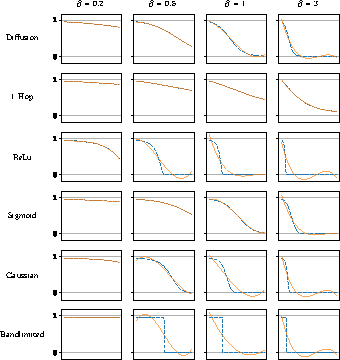
\includegraphics[width=0.9\linewidth]{Figures/cheb_approx.pdf}
    \caption[Chebyshev approximation accuracy visualisation]{\small{An order-3 Chebyshev polynomial approximation (orange) is compared to the true output of $J(x)$ (dashed blue) for several different filter types across various parameter settings. Note how the accuracy of the fit depends on both the filter function used and the value of $\beta$. Furthermore, the approximation can sometimes fall outside of the [0, 1] interval. }}
    \label{fig:cheb_approx}
\end{figure}


\subsection{A conjugate gradient method}

\label{sec:CGM}

The second approach we consider for computing the posterior mean is to use the Conjugate Gradient Method (CGM). First proposed in 1952, the CGM is part of the Krylov subspace family and is perhaps the most prominent iterative algorithm for solving linear systems \citep{Hestenes1952}. In computational terms, the method only requires repeated forward multiplication of vectors by the coefficient matrix which, in the standard CGM, bust be PSD. It is therefore effective in applications where this process can be performed efficiently. 

In brief, the CGM seeks to solve the linear system $\A \x = \bb$ by minimising, at the $k$-th iteration, some measure of error in the affine space $\x_0 + \mathcal{K}_k$ where $\mathcal{K}_k$ is the $k$-th Krylov subspace given by  

$$
\mathcal{K}_k = \text{span}\big(\rr_0, \; \A \rr_0, \, ..., \, \A^{k-1} \rr_0 \big)
$$

The residual $\rr_k$ is given by 

$$
\rr_k = \bb - \A \x
$$

and the $k$-th iterate of the CGM minimises 

$$
\phi(\x) = \frac{1}{2} \x^\top \A \x  - \x^\top \bb
$$

over $\x_0 + \mathcal{K}_k$ \citep{Kelley1995}. 

The CGM works best when the coefficient matrix $\A$ has a low condition number $\kappa$ (that is, the ratio between the largest and smallest eigenvalue is small) and, as such, a preconditioning step is often necessary. The purpose of a preconditioner is to reduce $\kappa$ by solving an equivalent transformed problem. This can be achieved by right or left multiplying the linear system by a preconditioning matrix $\PSI$. However, this likely means the coefficient matrix is no longer PSD, meaning the CGM cannot be used in its basic form. (Other approaches modified for non-PSD matrices exist, e.g. the CGNE or GIMRES \citep{Elman1982, Saad1986}). A preconditioner can also multiply the coefficient matrix on the right by a preconditioner $\PSI^\top$ and on the left by $\PSI$. This preserves the symmetry meaning we can continue to use the regular CGM. 

In our case, where the coefficient matrix is given by $\Big(\diag{\vecc{\Ss}} + \gamma  \HH^{-2}\Big)$, preconditioning will be essential for convergence. To see why, consider the definition of $\HH$ in equation (\ref{eq:graph_filter}). A low-pass filter function $g(\cdot)$ may be close to zero when applied to the high-frequency eigenvalues of the graph Laplacian, meaning elements of $\diag{\vecc{\G}}^{-2}$ may be very large. In the worst case, for example with a band-limited filter, the matrix $\HH$ will be singular, no matrix $\HH^{-2}$ will exist, and the condition number of the coefficient matrix will be, in effect, infinite. Therefore, the primary purpose of this subsection is to find a preconditioner that maintains efficient forward multiplication and is effective at reducing the condition number of the coefficient matrix.

References such as \cite{Saad2003} give a broad overview of the known approaches to finding a preconditioner. Standard examples include the Jacobi preconditioner which is given by the inverse of the coefficient matrix diagonal and is effective for diagonally dominant matrices, and the Sparse Approximate Inverse preconditioner \citep{Grote1997}. However, such preconditioners generally require direct evaluation of parts of the coefficient matrix or are computationally intensive to calculate.

In the following, we derive an effective symmetric preconditioner that allows forward multiplication of the coefficient matrix to be performed efficiently. First consider the transformed variable $\Z$, related to $\F$ in the following way.

\begin{equation}
    \label{eq:Z_transform}
    \F = \U_N \, (\G \circ \Z) \, \U_T^\top
\end{equation}

Here, $\Z$ can be interpreted as a set of Laplacian frequency coefficients, which are subsequently scaled according to the graph filter function, and then reverse Fourier transformed back into the node domain. Matrices $\Z$ which are distributed according to a spherically symmetric distribution, result in signals $\F$ which are smooth with respect to the graph topology. Since this transform filters out the problematic high-Laplacian frequency Fourier components, the system defined by this transformed variable $\Z$ is naturally far better conditioned.

By substituting this expression for $\F$ back into the likelihood in equation (\ref{eq:Y_given_F}), and the prior of equation (\ref{eq:F_prior}), one can derive a new expression for the posterior mean of $\Z$. This is done explicitly in \cref{the:Z_transform_bayes}. The end result is that the new linear system for the transformed variable $\Z$ is given by


\begin{equation}
    \label{eq:Z_post}
    \vecc{\Z} = \Big( \D_{\G} \big( \U_T^\top \otimes \U_N^\top \big)\, \D_{\Ss} \, \big(\U_T \otimes \U_N \big) \,\D_{\G} + \gamma \I_{NT} \Big)^{-1} \vecc{\G \circ \big(\U_N^\top \Y \U_T\big)}
\end{equation}

\noindent where we have abbreviated $\diag{\vecc{\G}}$ and $\diag{\vecc{\Ss}}$ as $\D_{\G}$ and $\D_{\Ss}$ respectively. Note that the conditioning of the coefficient matrix is greatly improved from the untransformed problem, as we will discuss in greater detail in \cref{sec:convergence}. Note also that the multiplication of a vector $\vecc{\RR}$ by the coefficient matrix can be computed efficiently as 

\begin{multline}
    \mat{\Big( \D_{\G} \big( \U_T^\top \otimes \U_N^\top \big)\, \D_{\Ss} \, \big(\U_T \otimes \U_N \big) \,\D_{\G} + \gamma \I_{NT} \Big) \, \vecc{\RR}} \\ = \gamma \RR + \G \circ \left(\U_N^\top \Big( \Ss \circ \big(\U_N (\G \circ \RR) \U_T^\top \big) \Big) \U_T\right) 
\end{multline}



This has $O(N^2T + NT^2)$ complexity at each step which may be reduced to $O(N^2T + NT \log T)$ in the case of T-V problems, and to $O\big(NT \log NT \big)$ for data residing on a grid (see \cref{box}). 

The linear system defined \cref{eq:Z_post} can be understood as a two-sided symmetrically preconditioned version of the original linear system given in \cref{eq:lin_system}. In particular, the new expression can be constructed by modifying the original system in the following way.

\begin{equation}
    \Big(\PSI^\top  \big(\D_{\Ss} + \gamma  \HH^{-2}\big) \, \PSI  \Big) \Big(\PSI^{-1}\, \vecc{ \F } \Big) = \PSI^\top \, \vecc{\Y},
\end{equation}

\noindent where

\begin{equation}
    \PSI =   \big(\U_T \otimes \U_N\big) \, \D_{\G}.
\end{equation}

Since preconditioning of the coefficient matrix on the left is achieved with $\PSI^\top$ and on the right with $\PSI$, symmetry is preserved. This ensures that one can continue to utilise algorithms tailored to work with PSD matrices. In algorithm \hyperlink{al:CGM}{\textbf{2}}, we outline a conjugate gradient method based on this new formulation. 

\begin{algorithm}[t]
    \hypertarget{al:CGM}{}
    \label{al:MVGKR}
    \caption{Conjugate gradient method with graph-spectral preconditioner}
    \begin{algorithmic}
        \vspace{0.15cm}
        \Require{Observation matrix $\Y \in \R^{N \times T}$}
        \vspace{0.05cm}
        \Require{Sensing matrix $\Ss \in \{0, 1\}^{N \times T}$}
        \vspace{0.05cm}
        \Require{Space-like graph Laplacian $\LL_N \in \R^{N \times N}$}
        \vspace{0.05cm}
        \Require{Time-like graph Laplacian $\LL_T \in \R^{T \times T}$}
        \vspace{0.05cm}
        \Require{Regularisation parameter $\gamma \in \R$}
        \vspace{0.05cm}
        \Require{Graph filter function $g(\, \cdot\, \,; \betaa)$}
        \vspace{0.25cm}
        \State{Decompose $\LL_N$ into $\U_N \LAM_L \U_N^\top$ and $\LL_T$ into $\U_T \LAM_T \U_T^\top$}
        \vspace{0.15cm}
        \State{Compute $\G \in \R^{N \times T}$ as $\G_{nt} = g \left(\lambda^{(N)}_n, \lambda^{(T)}_t; \, \betaa \right)$ }
        \vspace{0.15cm}
        \State{Initialise $\Z \in \R^{N \times T}$ randomly}
        \vspace{0.15cm}
        \State{$\RR \leftarrow \G \circ (\U_N^\top \Y \U_T) - \gamma \Z - \G \circ \Big( \, \U_N^\top \big(\Ss \circ (\U_N \, (\G \circ \Z) \, \U_T^\top) \big)  \, \U_T\Big)$}
        \vspace{0.15cm}
        \State{$\D \leftarrow \RR$}
        \vspace{0.15cm}
        \While{$|\Delta\RR| > \text{tol}$}
        \vspace{0.15cm}
        \State{$\A_D \leftarrow \gamma \D + \G \circ \Big( \, \U_N^\top \big(\Ss \circ (\U_N \, (\G \circ \D) \, \U_T^\top) \big)\, \U_T\Big) $}
        \vspace{0.15cm}
        \State{$\alpha \leftarrow  \tr{\RR^\top \RR} \, / \, \tr{\RR^\top \A_D \RR}$}
        \vspace{0.15cm}
        \State{$\Z \leftarrow  \Z + \alpha \D $}
        \vspace{0.15cm}
        \State{$\RR \leftarrow  \RR - \alpha \A_D $}
        \vspace{0.15cm}
        \State{$\delta \leftarrow \tr{\RR^\top \RR} \, / \, \tr{(\RR + \alpha \A_D)^\top (\RR + \alpha \A_D)}$}
        \vspace{0.15cm}
        \State{$\D \leftarrow  \RR + \delta \D $}
        \vspace{0.15cm}
        \EndWhile
        \vspace{0.25cm}
        \Ensure{$\U_N \, (\G \circ \Z) \, \U_T^\top$}
        \vspace{0.15cm}
    \end{algorithmic}
\end{algorithm}
 
\subsection{Real data experiments}

In this subsection, we evaluate our GSR method using a dataset consisting of daily new SARS-CoV-2 cases reported in 372 lower-tier local authorities across the United Kingdom from February 5, 2020, to March 18, 2023 (1138 days) taken from the UK government website\footnote{See \url{https://coronavirus.data.gov.uk/details/download}}. Specifically, we focused on the ``newCasesBySpecimenDateRollingRate" metric, which represents the daily number of cases reported per 100,000 residents in each local reporting authority over a 7-day rolling period. To create a graph, we used boundary data \footnote{Data from the Office for National Statistics \citep{ONS2019}}, setting adjacency matrix entries as $\A_{ij}$ to one if districts $i$ and $j$ share a border, and zero otherwise. Note, this graph construction strategy is fairly crude, with the underlying assumption being that virus spread occurs mainly between neighbouring regions. Perhaps a more sophisticated model could use data such as inter-region travel volumes to construct a graph, although such data was not easily available at the time of writing. \Cref{fig:covid} illustrates a snapshot of this dataset on December 1, 2020.


\begin{figure}[t]
    \begin{center}
        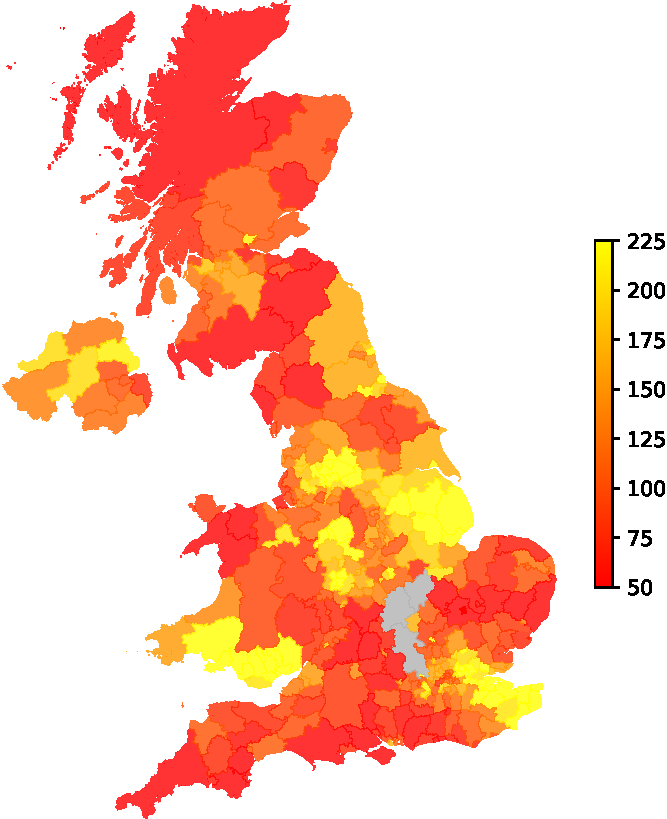
\includegraphics[width=0.6\linewidth]{Figures/UK_covid.pdf}
    \end{center}
    \caption[Snapshot of the Covid-19 case rate in the UK]{\small{The seven-day rolling rate of new Covid cases reported per 100,000 residents in each lower-tier local reporting authority in the United Kingdom on the 1st of December 2020. Missing data is indicated in grey.}}
    \label{fig:covid}
\end{figure}


Before beginning the experiments, we performed two preprocessing steps on the raw signal data. First, we took the logarithm of 10 plus the original case rate. This was to eliminate the long tail in the case rate histogram, transforming it to be closer to a Gaussian. We then normalised by subtracting the overall mean and dividing by the standard deviation. The resultant signal, of shape $372 \times 1138$, we refer to as $\Y_0$. Note that 4.8\% of the entries in $\Y_0$ were already missing from the original dataset (mostly occurring in the earlier stages of the pandemic).

The experiment was conducted as follows. First, we removed data from $\Y_0$ such that a total fraction $m$ was no longer present. This created two matrices: $\Y$, the partially observed signal with missing values filled with zeros; and $\Ss$, the corresponding binary sensing matrix. Data was removed in four distinct ways. First, individual elements of $\Y$ were selected uniformly at random for removal (`uniform'). Second, strings of 100 days, beginning at a random date, were removed for individual randomly selected districts (`strings'). Third, the entire time series for randomly chosen districts were removed (`districts'). Finally, the signal across every node at randomly selected dates was removed (`dates'). These four techniques for data removal are depicted for clarity in \cref{fig:missing_data}. For each technique, we solved the signal reconstruction problem using the GSR model described in this chapter and compared its performance to other baseline reconstruction strategies. In particular, for uniform and string removal, we compared it to linear interpolation in time and longitudinal averaging across all districts. For date removal, we compared it to interpolation in time only, since longitudinal averaging is not possible in this case. Finally, for district removal, we compared it to longitudinal averaging, since linear interpolation in time is not possible in this case. For each model, for each method of data removal, we measured the Root Mean Square Error (RMSE) across the reconstructed entries, over four increasing values of $m$. 


\begin{figure}[t]
    \begin{center}
        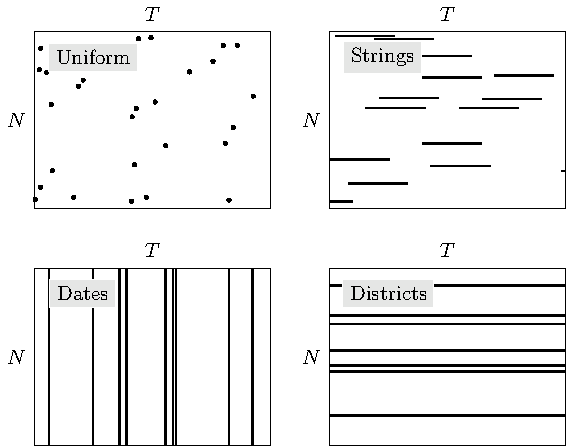
\includegraphics[width=0.6\linewidth]{Figures/missing.pdf}
    \end{center}
    \caption{\small{A visual depiction of the four ways we removed data. Black lines/dots indicate data that was removed. }}
    \label{fig:missing_data}
\end{figure}


\begin{table*}[t]
    \centering
    \footnotesize 
    % \def\arraystretch{1}
    \begin{tabular}{lcccccccccc}
    \toprule
    & \multicolumn{4}{c}{Uniform} & \phantom{a} & \multicolumn{4}{c}{Strings} \\
    \cmidrule{2-5} \cmidrule{7-10} 
    $m$ & 0.1   & 0.3 & 0.5 & 0.7 &&  0.1   & 0.3  & 0.5 & 0.7  \\ \midrule \rule{0pt}{0.5cm}
   Bayesian GSR & 0.037 & 0.040 & \colorbox{best!35}{0.048} & 0.081 && 0.230 &  \colorbox{best!35}{0.249} & \colorbox{best!35}{0.247} & \colorbox{best!35}{0.243} \\ \rule{0pt}{6ex} 
    Qiu et al noiseless & 0.040 & 0.043 & 0.054 & 0.092 && 0.242 & 0.255 & 0.254 & 0.251 \\ \rule{0pt}{6ex} 
    Qiu et al noisy & 0.037 & 0.041 & \colorbox{best!35}{0.048} & 0.080 && \colorbox{best!35}{0.229} &  \colorbox{best!35}{0.249} & 0.249 & 0.244 \\ 
    \rule{0pt}{6ex} 
    Linear interp & \colorbox{best!35}{0.034} & \colorbox{best!35}{0.039} &  0.049 & \colorbox{best!35}{0.070} && 0.540 & 0.531 & 0.520 & 0.526 \\ 
    \rule{0pt}{6ex}
    Longitudinal avrg & 0.350 & 0.348 &  0.347 & 0.348 && 0.341 & 0.350 & 0.356 & 0.347  \\[0.2cm] \midrule \rule{0pt}{4ex}
    & \multicolumn{4}{c}{Dates} & \phantom{a} & \multicolumn{4}{c}{Districts} \\
    \cmidrule{2-5} \cmidrule{7-10} 
    $m$ & 0.1   & 0.3 & 0.5 & 0.7 &&  0.1   & 0.3  & 0.5 & 0.7  \\ \midrule \rule{0pt}{0.5cm}
    Bayesian GSR & 0.038 & 0.055 & 0.058 & 0.075  && \colorbox{best!35}{0.202} & 0.249 & \colorbox{best!35}{0.271} & \colorbox{best!35}{0.273} \\ 
    \rule{0pt}{6ex} 
     Qiu et al noiseless & 0.041 & 0.060 & 0.062 & 0.079 && 0.210 &  0.257 & 0.281 & 0.282 \\ \rule{0pt}{6ex} 
    Qiu et al noisy & 0.037 & 0.040 & \colorbox{best!35}{0.048} & 0.081 && \colorbox{best!35}{0.202} &  \colorbox{best!35}{0.248} & 0.274 & \colorbox{best!35}{0.273} \\ \rule{0pt}{6ex} 
    Linear interp & \colorbox{best!35}{0.035} & \colorbox{best!35}{0.038} & \colorbox{best!35}{0.046} & \colorbox{best!35}{0.066} && NA & NA & NA & NA \\ \rule{0pt}{6ex}
    Longitudinal avrg & NA & NA & NA & NA && 0.318 & 0.333 & 0.347 & 0.345 \\[0.2cm] \bottomrule
    \end{tabular}
    \caption[Graph signal reconstruction real data results]{The RMSE for different reconstruction models and data removal techniques on the UK SARS-CoV-2 case rate dataset. For each fraction of missing data $m$, the best-performing model is highlighted in green. Entries where the model is not applicable are indicated by NA. }
    \label{tab:gsr_real_data_experiemnts} 
\end{table*}


In addition to the aforementioned reconstruction models, we also implemented the time-varying signal reconstruction models described in \cite{Qiu2017}. In this paper, the authors describe two alternative methods for reconstructing a time-varying graph signal representing a noiseless and a noisy case. The noiseless case seeks the reconstructed signal $\F$ that minimises their chosen smoothness metric subject to the constraint that it precisely interpolates the observed values of $\Y$. The noisy case, which is more similar to the model described in this paper, assumes a certain level of noise in the observed values and does not strictly interpolate. The results are shown in table \ref{tab:gsr_real_data_experiemnts}. 

The findings indicate that the graph-aware approaches exhibit significantly better performance, particularly for the `strings' and `districts' removal strategies. In particular, they outperform longitudinal averaging, underscoring the substantial benefits derived from integrating topological relationships between districts. Conversely, when individual dates are excluded, thus likely leaving only brief segments of the time series absent in any district, the GSR methods remain competitive, albeit linear interpolation shows marginally superior results. This outcome is anticipated for this dataset, considering the metric is computed using a 7-day rolling average, which naturally results in a smooth signal progression. Nevertheless, GSR stands out for its adaptability, applicable to various patterns of missing data.

Comparing the Bayesian GSR model presented in this study with the noiseless and noisy GSR models discussed in \cite{Qiu2017}, it emerges that both the noisy model and Bayesian GSR generally surpass the noiseless model. This disparity is likely attributable to the significant noise in the real data, which disproportionately influences the reconstruction predictions. The performances of Bayesian GSR and Qiu’s noisy model are closely matched, with Bayesian GSR slightly outperforming in a small majority of scenarios.

 
\section{Convergence properties}

\label{sec:convergence}

In this section, we conduct a thorough theoretical analysis of the convergence properties of both the SIM and the CGM. As we will demonstrate, their respective convergence rates are heavily influenced by the values of the hyperparameters $\beta$, which describes the strength of the graph filter, $\gamma$, which determines the regularization strength, and $m=|\mathcal{S}'|/NT$, which represents the fraction of values missing from the original graph signal. This helps explain the empirical convergence behaviour and offers insight into trade-offs when it comes to hyperparameter selection. Furthermore, it allows users to make an informed decision about selecting an appropriate method, considering the inherent characteristics of their specific problem. 

It is well-known that the worst-case number of iterations required to reduce the error below some specific tolerance level for matrix splitting methods is inversely proportional to $-\log \rho(\M^{-1}\N)$, where $\rho(\cdot)$ denotes the spectral radius (absolute value of the maximum eigenvalue) of a matrix \citep{Demmel1997}. For completeness, we provide a brief proof of this in \cref{the:SIM_convergence}. In the specific context of our graph signal reconstruction algorithm as outlined in \cref{sec:SIM}, $\M$ and $\N$ have the following values.  


$$
\M = \big(\U \D_\J \U^\top\big)^{-1}, \aand \N = \D_{\Ss'}
$$

where  $\U = \U_T \otimes \U_N$, $\D_\J = \diag{\vecc{\J}}$, and $\D_{\Ss'} = \diag{\vecc{\Ss'}}$. Therefore, the number of iterations required for convergence of the SIM scales as


\begin{equation}
    \label{eq:n_SIM}
    n_\text{SIM} \propto  -\frac{1}{\log\rho\left(\U \D_\J \U^\top \D_{\Ss'} \right)}
\end{equation}

Note that the matrix $\J$ [see \cref{eq:Jnt} for its definition] has entries that depend on both the regularisation parameter $\gamma$ and the spectral scaling matrix $\G$, which is itself a function of the graph filter parameter(s) $\beta$ [see \cref{eq:Gba,eq:Gba2}]. The matrix $\D_{\Ss'}$ has entries that depend on the structure of the missing data in the graph signal. Therefore should we expect that the spectral radius, $\rho$, and consequently the number of steps required for convergence, $n_\text{SIM}$, can be affected by all three.  

Similarly, in the conjugate gradient method, the worst-case number of steps required to achieve a specific termination criterion is well-known to be proportional to $\sqrt{\kappa}$, where $\kappa$ represents the condition number of the coefficient matrix, i.e. the ratio between the largest and smallest eigenvalue \cite{Kelley1995}. In our particular scenario, the coefficient matrix is provided in \cref{eq:Z_post}. Therefore, we should expect that the number of iterations required for convergence of the CGM will scale as

\begin{equation}
    \label{eq:n_CGM}
     n_\text{CGM} \propto \sqrt{\kappa \left(  \, \D_\G \U^\top \D_{\Ss} \U \D_\G + \gamma \I_{NT} \; \right)}
\end{equation}

where $\D_\G = \diag{\vecc{\G}}$. Once again, this expression contains the matrix $\G$, which depends on the strength of the graph filter function parameter $\beta$, the matrix $\D_{\Ss}$, which depends on the structure of this missing data, and the precision parameter $\gamma$. Consequently, we should expect that, in general, convergence of the CGM is affected by all three of these variables. 

Whilst it is not possible in general to obtain an analytic expression for $\rho$ or $\kappa$ as a function of $\gamma, \beta$ and $m$, we can nonetheless gain useful insight into how each of these variables can be expected to affect convergence. We achieve this by considering two distinct limits: one in which the graph filter is very strong (i.e. $\beta$ is very large) and one in which the graph filter is very weak (i.e. $\beta$ is very small). 

\subsection{Upper bound on convergence: the weak filter limit}

\label{sec:wfl_derivation}

Consider the limiting case of a weak filter, where all spectral components are allowed to pass through unaffected. In this case, a graph filter $\HH$ [see \cref{eq:graph_filter}], which appears in the prior distribution for $\F$ [see \cref{eq:F_prior}], becomes the identity matrix $\I_{NT}$. This means no topological information is included in the prior for $\F$ at all. Given the definitions of the graph filters in \cref{tab:iso_filters,tab:anis_filters_2d}, we can conceptualise this as the limit where the parameter characterising the graph filter $\beta \rightarrow 0$ (or, more generally, the limit as $\betaa \rightarrow [0, 0]$ for an anisotropic graph filter). Since all spectral components are maintained, every element of the spectral scaling matrix $\G$ will be equal to one. Given \cref{eq:Jnt}, this further implies the every entry in the matrix $\J$ becomes $1 / (1 + \gamma)$. 

$$
\lim_{\beta \rightarrow 0} \; \D_\G = \I_{NT}, \aand \lim_{\beta \rightarrow 0} \; \D_\J = \frac{1}{1 + \gamma} \I_{NT}
$$

Now consider the spectral radius $\rho$ of the update matrix in the SIM. Given this limiting value of $\D_\J$, it can be directly evaluated as

\begin{equation}
    \lim_{\beta \rightarrow 0} \; \rho\Big(\U \D_\J \U^\top \D_{\Ss'} \Big)
    = \frac{1}{1 + \gamma} \rho\Big(\D_{\Ss'} \Big)
    = \frac{1}{1 + \gamma} \label{eq:beta_lim_0} 
\end{equation}


Next, consider the condition number $\kappa$ of the coefficient matrix in the CGM. Again, since in this limit $\D_\G = \I$, it can be directly evaluated as 


\begin{equation}
    \lim_{\beta \rightarrow 0} \; \kappa \left(  \, \D_\G \U^\top \D_{\Ss} \U \D_\G + \gamma \I \; \right)
    = \kappa  \left(  \, \U^\top \left( \D_{\Ss} + \gamma \I \right) \U \; \right)
    = \frac{1 + \gamma}{\gamma}
\end{equation}

 Given \cref{eq:n_SIM,eq:n_CGM}, we can characterise the number of iterations required to reach some convergence criterion in the weak filter limit for the SIM and CGM respectively as

 \begin{equation}
    \label{eq:n_WFL}
    \lim_{\beta \rightarrow 0} \;  n_\text{SIM} \, \propto \;\;  \frac{1}{\log(1 + \gamma)}, \;\;  \aand  \;\; \lim_{\beta \rightarrow 0} \;  n_\text{CGM} \, \propto \;\;\;  \sqrt{\frac{1}{\gamma} + 1}
 \end{equation}

These expressions imply that when $\gamma$ is large, both methods converge quickly. However, they both see the number of iterations increase to infinity as $\gamma \rightarrow 0$. To characterise this more precisely, consider the Taylor expansion of each expression around $\gamma = 0$.  

\begin{equation}
    \lim_{\beta \rightarrow 0} \;  n_\text{SIM}  \;  \propto \gamma^{-1} \, + \, O(\gamma), \;\; \aand \;\; \lim_{\beta \rightarrow 0} \;  n_\text{CGM} \propto \, \gamma^{-1/2} \, + \, O\left(\gamma^{1/2}\right) 
\end{equation}


As visible, dominant behaviour for small $\gamma$ follows $O(\gamma^{-1})$ for the SIM and $O(\gamma^{-1/2})$ for the CGM.

\subsection{Lower bound on convergence: the strong filter limit}

Consider now the limiting case of a strong filter as applied to a signal on a fully connected Cartesian product graph. In this case, every spectral component is filtered out except the the first Laplacian frequency component $\uu_1^{(T)} \otimes \uu_1^{(N)}   \propto \mathbf{1}$ (also known as the bias), with eigenvalue $\lambda_1^{(T)} + \lambda_1^{(N)} = 0$, which passes through the filter unaffected. When a filter of this kind is used in the prior for $\F$, it effectively forces predictions that are constant across all nodes. Given the definitions of the graph filter functions given in \cref{tab:iso_filters,tab:anis_filters_2d}, we can associate this with the limit as $\beta \rightarrow \infty$. Here, the effect of applying the graph filter to a generic graph signal $\vecc{\Y}$ is to extract the mean, that is 

$$
\HH \vecc{\Y} = \frac{1}{NT} \left(\sum_{n, t} \Y_{nt}\right) \mathbf{1}
$$


In this case, the spectral scaling matrix $\G$ has entries that are zero for all elements except (1, 1) which has the value one. Similarly, the matrix $\J$ has the value $1 / (1 + \gamma)$ at element (1, 1) and zeros elsewhere. This implies that


$$
\lim_{\beta \rightarrow \infty} \; \D_\G = \mathbf{\Delta}, \aand \lim_{\beta \rightarrow \infty} \; \D_\J = \frac{1}{1 + \gamma} \mathbf{\Delta}, 
$$

where $\mathbf{\Delta}$ is an $NT \times NT$ matrix given by

$$
\mathbf{\Delta} = \begin{bmatrix}
    1 & 0 & 0 & \dots \\
    0 & 0 & 0 &  \\
    \vdots & & & \ddots
\end{bmatrix}
$$

 In the case of the SIM, the spectral radius of $\M^{-1}\N$ in this limit is therefore given by

\begin{align*}
    \lim_{\beta \rightarrow \infty} \; \rho\Big(\U \D_\J \U^\top \D_{\Ss'} \Big) &= \frac{1}{1 + \gamma} \rho\Big(\U \mathbf{\Delta} \U^\top \D_{\Ss'} \Big)
\end{align*}

Note that 

\begin{equation*}
    \U \mathbf{\Delta} \U^\top = \uu_1 \uu_1^\top  = \frac{1}{NT} \OO_{NT}
\end{equation*}

where $ \OO_{NT}$ is an $NT \times NT$ matrix of ones. Therefore the spectral radius is given by 

\begin{align*}
    \lim_{\beta \rightarrow \infty} \; \rho(\U \D_\J \U^\top \D_{\Ss'}) &= \frac{1}{NT (1 + \gamma) } \; \rho \left( \begin{bmatrix}
        \vecc{\Ss'}^\top \\ \vecc{\Ss'}^\top \\ \dots \\ \vecc{\Ss'}^\top
    \end{bmatrix} \right)
\end{align*}

Since the matrix in brackets is just the vector $\vecc{\Ss'}^\top$ repeated in every row it is surely of rank one and therefore must have an eigenvalue of 0 with multiplicity $NT - 1$. This implies that the only non-zero eigenvalue (and therefore the spectral radius $\rho$) is given by its trace, which is $\sum_{n, t}\Ss'_{nt} = |\mathcal{S}'|$. Denoting  $m=|\mathcal{S}'|/NT$, this can be expressed as 

\begin{equation}
    \label{eq:beta_lim_inf}
    \lim_{\beta \rightarrow \infty} \; \rho(\U \D_\J \U^\top \D_{\Ss'}) \, = \, \frac{1}{1 + \gamma} \frac{|\mathcal{S}'|}{NT} \, = \, \frac{m}{1 + \gamma}
\end{equation}

Now consider the condition number $\kappa$ of the CGM coefficient matrix. In the strong filter limit, this is given by  

\begin{align}
    \lim_{\beta \rightarrow \infty} \quad \kappa \left(  \, \D_\G \U^\top \D_{\Ss} \U \D_\G + \gamma \I \; \right)  &= \kappa  \left(  \, \mathbf{\Delta} \U^\top \D_{\Ss} \U \mathbf{\Delta}  + \gamma \I \; \right) \notag \\[0.3cm]
    &= \kappa  \left(  \, 
    \begin{bmatrix} 
        \uu_1^\top \\ 
        \zero^\top \\
        \vdots \\ 
        \zero^\top 
    \end{bmatrix} \D_{\Ss}  \Big[ \uu_1, \, \zero, \, \dots, \,\zero \Big]
    + \gamma \I \; \right) \notag \\[0.2cm]
    &= \kappa  \left(  \, \frac{1}{NT}  \begin{bmatrix}
        |\mathcal{S}| & 0 & 0 & \dots \\
        0 & 0 & 0 &  \\
        \vdots & & & \ddots
    \end{bmatrix}   + \gamma \I \; \right) \notag \\[0.3cm]
    &= \frac{1 - m + \gamma}{\gamma}
\end{align}

Given \cref{eq:n_SIM,eq:n_CGM}, we can write the scaling rate for the number of iterations in the SIM and CGM respectively. 

\begin{equation}
    \label{eq:n_SFL}
    \lim_{\beta \rightarrow \infty} \;  n_\text{SIM} \, \propto \;\;  \frac{1}{\log(1 + \gamma) - \log m}, \;\; \aand \;\;  \lim_{\beta \rightarrow \infty} \;  n_\text{CGM} \, \propto \;\, \sqrt{\frac{1 - m + \gamma}{\gamma}}
\end{equation}


A key feature of these expressions is that increasing the fraction of missing data $m$ will increase $n_\text{SIM}$, but decrease $n_\text{CGM}$. Note also that, in the case of a strong filter, the number of iterations required for convergence of the CGM, $n_\text{CGM}$, still goes to infinity as $\gamma \rightarrow 0$. However, this behaviour is no longer present for $n_\text{SIM}$, which tends towards a constant value of $-1/\log m$. Taking a Taylor series expansion of both expressions about $\gamma=0$ demonstrates the asymptotic behaviour in terms of $\gamma$ more clearly. 

\begin{equation*}
    \lim_{\beta \rightarrow \infty} \;  n_\text{SIM} \, \propto \;\;  -\frac{1}{\log m} + O\left(\gamma\right), \;\; \aand \;\; \lim_{\beta \rightarrow \infty} \;  n_\text{CGM} \, \propto \, \left(\frac{\gamma}{1 - m} \right)^{-1/2} \, + O\left(\gamma^{1/2}\right) 
\end{equation*}


In particular, at small $\gamma$, the CGM still runs with complexity proportional to $\gamma^{-1/2}$ whereas the SIM does not involve $\gamma$ to a negative power at all. Note that $m$ cannot scale arbitrarily close to zero or one, since it will surely be between $1/NT$ and $1 - 1/NT$. 


\subsection{Practical implications and method selection}

\label{sec:GSR_convergence_implications}

In the preceding two sections, we have derived several formulae that characterise the convergence behaviour of both the CGM and the SIM in the limiting case of a strong and weak filter, where $\beta \rightarrow \infty$ and $\beta \rightarrow 0$ respectively. For the sake of clarity, we have consolidated the critical expressions in \cref{tab:conv_SIM_CGM}. In this section, we take a closer look at these expressions and distil the key features that are relevant for implementing these methods in practice.


\begin{table*}[t]
    \centering
    \def\arraystretch{1.5}
    \begin{tabular}{@{}cccccc}
    \toprule
    & \multicolumn{2}{c}{$n_\text{SIM}$} & \phantom{abc} & \multicolumn{2}{c}{$n_\text{CGM}$} \\
    \cmidrule{2-3} \cmidrule{5-6}
                               & All $\gamma$   & Small $\gamma$   &&  All $\gamma$   & Small $\gamma$ \\ \midrule \rule{0pt}{1cm}
    $\beta \rightarrow 0$      & $ \displaystyle \frac{1}{\log(1 + \gamma)}$   & $\displaystyle \gamma^{-1}$    &&    $\displaystyle \sqrt{\frac{1 + \gamma}{\gamma}}$ & $\displaystyle \gamma^{-1/2}$    \\ \rule{0pt}{6ex}
    $\beta \rightarrow \infty$ & $\displaystyle \frac{1}{\log(1 + \gamma) - \log m}$ & $\displaystyle -\frac{1}{\log m}$    &&  $\displaystyle \sqrt{\frac{1 - m + \gamma}{\gamma}}$ & $\displaystyle \left(\frac{\gamma}{1 - m} \right)^{-1/2}$ \\[0.5cm] \bottomrule 
    \end{tabular}
    \caption[The scaling behaviour of the number of steps required for convergence as a function of $\gamma$ and $m$.]{The scaling behaviour of the number of steps required for convergence is shown as a function of $\gamma$ and $m$. The upper row gives the behaviour in the limit of a weak filter, and the lower row gives the behaviour in the limit of a strong filter. We also show the dominant term in the Taylor expansion about $\gamma=0$ (``small $\gamma$" columns) which gives a clearer picture of the asymptotic behaviour as $\gamma \rightarrow 0$. }
    \label{tab:conv_SIM_CGM} 
\end{table*}

First consider the value of $\gamma$, which enters the model via \cref{eq:F_prior}, and acts as a strictly positive regularisation parameter. For both the SIM and CGM, smaller values of $\gamma$ will universally increase the total number of iterations. This can be proven by taking the partial derivative of each expression with respect to $\gamma$, and demonstrating that the resulting expressions are negative for all valid values of $\gamma$ and $m$. For completeness, we perform this explicitly in the proof of \cref{the:gamma_deriv_negative}. Furthermore, the number of iterations will tend towards infinity as $\gamma \rightarrow 0$ in all cases except an asymptotically strong filter with the SIM. When the filter is weak, we should expect that the number of iterations grows faster for the SIM than the CGM as $\gamma$ approaches zero. This can be seen from the Taylor series expansion about $\gamma = 0$, which has a dominant term of $\gamma^{-1}$ for the SIM and $\gamma^{-1/2}$ for the CGM. When $\gamma$ is large we should expect fast convergence for both the SIM and CGM regardless of the value of the other hyperparameters. 

Consider now the parameter $\beta$, which characterises the strength of the graph filter, and also enters the model in the prior for $\F$ in \cref{eq:F_prior}. For both the SIM and CGM, higher values of $\beta$, which more aggressively filter out high-frequency spectral components, are associated with faster convergence. In other words, like $\gamma$, increasing $\beta$ will decrease the number of iterations required to reach a fixed termination condition. This is evidently true since the expressions for $n_\text{SIM}$ and $n_\text{CGM}$ are lower when $\beta \rightarrow \infty$ than they are when $\beta \rightarrow 0$, for any valid value of $0 \leq m \leq 1$. It is also reasonable to expect that the number of iterations will decrease monotonically as $\beta$ is increased, however, we provide no formal proof of this. In contrast to the behaviour of $\gamma$, however, these two bounds are still both finite meaning that, the number of steps required for convergence remains finite as $\beta \rightarrow 0$. 

Whilst the convergence rates of both the SIM and CGM have the same directional response to changes in $\gamma$ and $\beta$, they display the opposite behaviour when $m$ is varied. In particular, a higher proportion of missing value in $\Y$, corresponding to an increasing value of $m$, causes the number of iterations to rise for the SIM but fall for the CGM, at least in the limit of a strong filter as $\beta \rightarrow \infty$. This can be shown explicitly by taking the partial derivative of $n_\text{SIM}$ and $n_\text{CGM}$ with respect to $m$ and demonstrating that it is universally positive for the former and negative for the latter (which we show in \cref{the:m_deriv}). While $m$ has no effect for either the SIM or CGM in the limit as $\beta \rightarrow 0$, we can reasonably expect that it will have \textit{some} effect for intermediate values of $\beta$. This insight is especially important since, unlike $\gamma$ and $\beta$, $m$ is a feature of the data rather than an adjustable hyperparameter. 

\subsection{Experimental validation}

In order to verify aspects of this theoretically predicted behaviour, we ran several experiments using synthetic data. In particular, we generated two random fully connected graphs, each with 50 nodes, and take their Cartesian product to create a product graph with 2500 nodes. Next, we generated a random $50 \times 50$ matrix of i.i.d. Gaussian noise with unit variance and chose a fraction $m$ to be removed uniformly at random to generate an observed graph signal $\Y \in \R^{50 \times 50}$ and corresponding binary sensing matrix $\Ss \in \{0, 1\}^{50 \times 50}$. Next, we set a prior for the underlying smooth signal $\F$ with precision $\gamma$ using an isotropic diffusion filter (see \cref{tab:iso_filters}) with parameter $\beta$. We then solved the graph signal reconstruction problem using both the SIM and CGM and counted the number of iterations required to reach a termination condition. Specifically, for the SIM, we terminate when $\Delta\F$ has a root mean square value of $10^{-8}$, and, for the CGM, when the residual has a root mean square value of $10^{-5}$, which we empirically determined resulted in similar final precision. In the following experiments, we completed this procedure for various values of $m$, $\beta$ and $\gamma$, and compared the empirical number of iterations required for convergence against the theoretical predictions determined in \cref{sec:convergence}. 
 
\subsubsection{Experiment 1: testing the strong and weak filter limits}

In the first experiment, we fix $\beta$ at zero and $\infty$, and measure the number of iterations required for convergence over a range of values of $m$ and $\gamma$. Since these correspond to the weak and strong filter limits respectively, we expect that the convergence rate should be bounded by a function proportional to those given in \cref{tab:conv_SIM_CGM}. First, we set $\beta=0$. Note that, in this case, $m$ does not affect the convergence rate of the SIM or CGM (which we also find empirically to be the case). We therefore varied $\gamma$ alone in 50 logarithmically spaced increments from $10^{-4}$ to $10^2$. The results are shown in \cref{fig:gamma_2d_plot}. As is visible, the functions broadly follow the expected convergence rate given by the theoretical prediction, performing slightly better in practice in both cases. Note that this is the expected behaviour since the limits give a \textit{worst case} scaling rate. In both cases, we also scaled the theoretical prediction (corresponding to a vertical shift in the log-log plot) to fit the experimental data. This is also valid since the theoretical predictions give a function proportional to the number of iterations rather than the number of iterations itself. For the SIM, this factor was approximately 10, and for the CGM this factor was approximately 4.5. 
 

\begin{figure}[t]
    \begin{center} 
    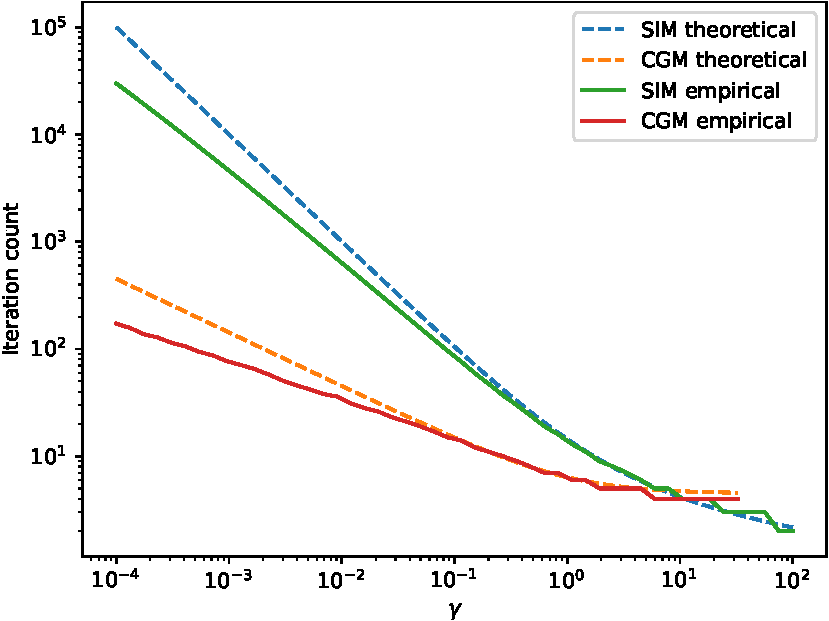
\includegraphics[width=0.7\linewidth]{Figures/gamma_plot_2d.pdf}
    \end{center}
    \caption{\small{The number of iterations required for convergence in the weak filter limit for the SIM and CGM both theoretically and empirically, as a function of $\gamma$.}}
    \label{fig:gamma_2d_plot}
\end{figure}


For the second part of experiment 1, we set $\beta = \infty$, corresponding to the strong filter limit. In this case, we expect the number of iterations to be a function of both $m$ and $\gamma$ as specified in \cref{tab:conv_SIM_CGM}. Therefore, we varied $\gamma$ in 50 logarithmically spaced increments from $10^{-6}$ to $10^2$ and $m$ in 50 linearly spaced increments from 0.01 to 0.99. For each unique pair of $m$ and $\gamma$, we then counted the number of iterations required for convergence and compared this to the theoretical predictions. The results are shown in \cref{fig:m_gamma_3d_plot}. Again, the empirical results broadly follow the theoretical functions which, as before, are scaled to fit the data. As with the weak filter limit, we again see that the empirical scaling rate is slightly better than the worst-case theoretical prediction. 

\begin{figure}[t]
    \begin{center} 
    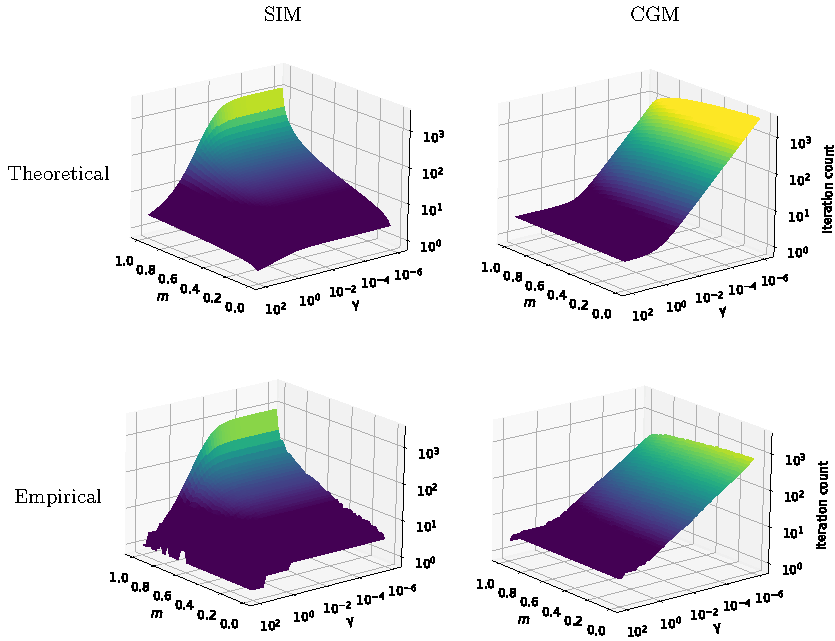
\includegraphics[width=\linewidth]{Figures/m_gamma_3d_plot.pdf}
    \end{center}
    \caption[Strong Filter Limit convergence experiments]{\small{The number of iterations required for convergence is shown both theoretically and empirically for the SIM and CGM in the strong filter limit, where $\beta=\infty$. In this case, each plot is a function of both $m$ and $\gamma$. The colourmap corresponds to vertical height and is normalised across each plot to aid comparison. }}
    \label{fig:m_gamma_3d_plot}
\end{figure}


\subsubsection{Experiment 2: Testing intermediate values of \texorpdfstring{$\beta$}{beta}}


In the second experiment, we test the number of iterations required for convergence for intermediate values of $\beta$. Note that the analysis carried out in \cref{sec:convergence} applies only for extremal values of $\beta$, meaning the intermediate behaviour is not clearly defined, and will depend on the filter chosen in practice. This was carried out for three values of $m$: 0.05, 0.5 and 0.95, representing low, medium and high prevalence of missing data respectively. For each value of $m$, we compute the solution using both algorithms over a grid of 50 $\beta$ values and 50 $\gamma$ values which were logarithmically spaced between $10^{-1}$-$10^2$ and $10^{-4}$-$10^1$ respectively. The results are shown in \cref{fig:3d_iteration_plots}. 


\begin{figure}[t]
    \begin{center} 
    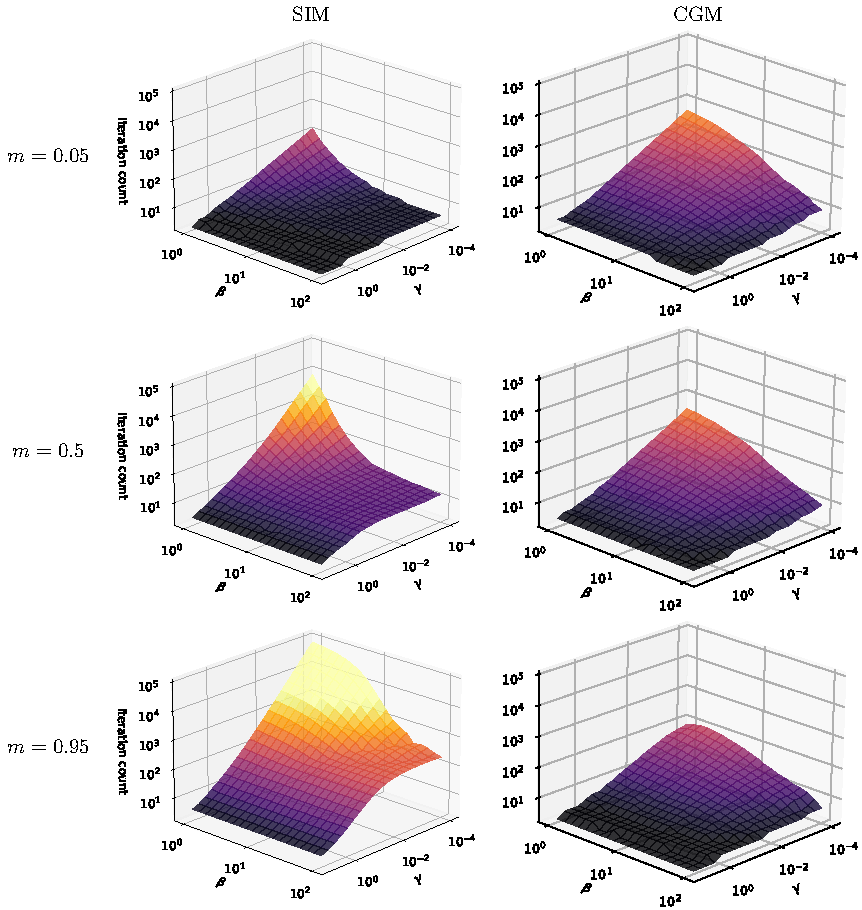
\includegraphics[width=\linewidth]{Figures/3d_iterations.pdf}
    \end{center}
    \caption[Convergence experiments]{\small{Six 3D surfaces are shown representing the number of iterations required for convergence for three values of $m$ for both the SIM and CGM algorithms. In each plot, the $x$-axis represents the filter parameter $\beta$, and the $y$-axis represents the regularisation parameter $\gamma$. The colourmap, which is normalised equally across all plots, tracks the vertical height. }}
    \label{fig:3d_iteration_plots}
\end{figure}

This experiment validates several key aspects of the theoretical convergence analysis. Firstly, notice that the basic behaviour that the number of iterations rises in all cases as $\beta$ and $\gamma$ get closer to zero. Furthermore, in all cases, regardless of the value of $m$ or $\beta$, convergence is very fast when $\gamma$ is large. We also observe the predicted behaviour that the number of iterations plateaus as a function of decreasing $\gamma$ when $\beta$ is large for the SIM while it continues to increase for the CGM. However, for this data, the CGM level seems to remain below that of the SIM in this limit. 

One key result of this experiment that aligns with the theoretical prediction is that convergence is accelerated as $m$ rises for the CGM but convergence slows as $m$ rises for the SIM. In particular, for this dataset, $n_\text{SIM} \leq n_\text{CGM}$ for all values of $\gamma$ and $\beta$ when $m=0.05$, but $n_\text{CGM} \leq n_\text{SIMM}$ for all values of $\gamma$ and $\beta$ when $m=0.95$. This is particularly impactful as it strongly indicates the CGM should be preferable when data is sparsely observed and the SIM should be preferable when the data is densely observed. 


\section{Conclusions}

In this chapter, we have addressed the problem of Graph Signal Reconstruction (GSR) on two-dimensional undirected Cartesian product graphs. We began by reviewing existing literature on product graphs, including eigendecomposition of their respective Laplacians \citep{Imrich2000} and discussed the significance of the Cartesian product in particular, which leads to a natural definition of the two-dimensional GFT. Given this, we proposed a formulation for anisotropic two-dimensional graph filters, which builds on the work of \cite{Ioannidis2016} who define the notion of `space-time kernels' for time-varying graph signals, and the T-V framework of \cite{Grassi2018, Isufi2017, Loukas2016}, where the authors discuss joint time-vertex filters. Our formulation provides a modest generalisation, by considering two generic graphs in the product, rather than one necessarily representing time. 

We then used the concept of anisotropic filters to define a Bayesian model for the reconstruction of signals on Cartesian product graphs. This extends related work on univariate GSR \citep{Narang2013,Romero2017b} and Time-Vertex GSR \citep{Qiu2017,Ioannidis2016} by considering arbitrary undirected topologies for each factor graph. Our model assumes that the observed signal, $\Y \in \R^{N \times T}$ is a partial observation of a smooth latent signal $\F$, with white Gaussian noise. By specifying the expected frequency profile of $\F$ with a filter-based prior, the model output is a Gaussian posterior over the latent signal $\F$. 

The posterior mean is naturally expressed as a linear system of size $(NT \times NT)$. In order to solve this efficiently, we proposed specialised versions of the classic matrix splitting and conjugate gradient algorithms that leverage the Kronecker structure of the relevant matrices. This resulted in two alternative algorithms, namely the Stationary Iterative Method (SIM) and Conjugate Gradient Method (CGM) both of which can be solved with a complexity of $O(N^2T + NT^2)$ per iterative step. In the case of the SIM, we also demonstrated how Chebyshev polynomials, which are often used in distributed GSP models \citep{Shuman2018}, can be leveraged to perform this in a distributed and/or eigendecomposition-free manner. 

In the latter part of this chapter, we focused on a detailed analysis of the convergence behaviour of the SIM and CGM. In particular, we considered how the number of iterations required for convergence is affected by the hyperparameters $\beta$ and $\gamma$, and the proportion of missing data, $m$. One key finding is that, while both algorithms experience slower convergence when the regularisation parameter $\gamma$ is small, the CGM has superior asymptotic performance as $\gamma \rightarrow 0$, with the number of iterations scaling as $\gamma^{-1/2}$ as compared to $\gamma^{-1}$. We also investigated how the proportion of missing data, $m$, impacts convergence. Interestingly, the SIM and CGM exhibit contrasting directional behaviour. Specifically, the CGM tends to be more suitable when the proportion of missing data is high, whereas SIM is generally preferable when it is low.


% We demonstrated the utility of this model on a dataset comprising daily measurements of SARS-CoV-19 across local districts in the UK from February 2020 to March 2023. Our GSR model had the flexibility to reconstruct missing data in every scenario, outperforming linear interpolation and longitudinal averaging when strings of dates were removed at each district, or entire districts were removed. 



\chapter{Signal Reconstruction on Cartesian Product Graphs}

\label{chap:reg_and_rec}

\lhead{Chapter 4. \emph{Regression and Reconstruction on Cartesian Product Graphs}}


In this chapter we explore a class of reconstruction algorithms as applied to signals defined on the nodes of a Cartesian product graph. In particular, we pose the reconstruction task in terms of Bayesian inference of an underlying signal given a noisy partial observation, and investigate scalable methods for obtaining the posterior mean. We begin in \cref{sec:reg_and_rec_intro} by reviewing the concept of a graph product, and explain why we choose to look specifically at the Cartesian product. We also review how concepts from standard one-dimensional graph signal processing such as the GFT and spectral filtering can be extended to the two dimensional case. In \cref{sec:gsr_cpg} we introduce the statistical model defining GSR on a Cartesian product graph, and derive two alternative methods for solving for the posterior mean. These comprise a Stationary Iterative Method (SIM) and a Conjugate Gradient Method (CGM). In each case, we show how graph spectral considerations can be leveraged to increase their convergence rate, and make use of the properties of the Kronecker product to complete each iteration efficiently. Finally, in section \ref{sec:convergence}, we analyse the convergence properties of each method in depth and derive how the rate of convergence is affected by the hyperparameters. In particular, we show how the optimal choice of method depends on the value of said hyperparameters and offer some rules-of-thumb for selecting a method in practice. 




\section{Graph Products}

\label{sec:reg_and_rec_intro}

In this chapter, we will be primarily concerned with signal processing on \textit{Cartesian product graphs}. This special class of graph finds applications in numerous areas, such as video, hyper-spectral image processing and network time series problems. However, the Cartesian product is not the only way to consistently define a product between two graphs. In this section we formally introduce the concept of a graph product, examine  some prominent examples, and explain why we choose to look specifically at the Cartesian graph product.

\subsection{Basic definitions}

\label{sec:graph_products_defined}

In the general case, consider two undirected graphs $\mathcal{G}_A = (\mathcal{V}_A, \mathcal{E}_A)$ and $\mathcal{G}_B = (\mathcal{V}_B, \mathcal{E}_B)$ with vertex sets given by $\mathcal{V}_A = \{a \in \mathbb{N} \, | \, a \leq A \}$ and $\mathcal{V}_B = \{b \in \mathbb{N} \, | \, b \leq B \}$ respectively. (In this context we do not regard zero to be an element of the natural numbers). A new graph $\mathcal{G}$ can be constructed by taking the product between $\mathcal{G}_A$ and $\mathcal{G}_B$. This can be generically written as follows.

\begin{equation}
    \mathcal{G} = \mathcal{G}_A \, \diamond \, \mathcal{G}_B = (\mathcal{V}, \, \mathcal{E})
\end{equation}

For all definitions of a graph product, the new vertex set $\mathcal{V}$ is given by the Cartesian product of the vertex sets of the factor graphs, that is

\begin{equation}
    \mathcal{V} = \mathcal{V}_A \times \mathcal{V}_B = \{(a, \, b) \in \mathbb{N}^2 \, | \, a \leq A \; \text{and} \; b \leq B \}
\end{equation}


Typically, vertices are are arranged in lexicographic order, in the sense that $(a, \, b) \leq (a',\, b')$ iff $a < a'$ or ($a = a'$ and $b \leq b'$) \citep{Harzheim2005}. Each consistent rule for constructing the new edge set $\mathcal{E}$ corresponds to a different definition of a graph product. In general, there are eight possible conditions for deciding whether two nodes $(a, \, b)$ and $(a',\,  b')$ are to be connected in the new graph.


\begin{table}[h]
    \def\arraystretch{1.5}
    \centering
    \begin{tabular}{lclc}
        1. & $[a, \, a'] \in \mathcal{E}_A$    & and & $b = b'$                          \\
        2. & $[a, \, a'] \notin \mathcal{E}_A$ & and & $b = b'$                          \\
        3. & $[a, \, a'] \in \mathcal{E}_A$    & and & $[b, \, b'] \in \mathcal{E}_B$    \\
        4. & $[a, \, a'] \notin \mathcal{E}_A$ & and & $[b, \, b'] \in \mathcal{E}_B$    \\
        5. & $[a, \, a'] \in \mathcal{E}_A$    & and & $[b, \, b'] \notin \mathcal{E}_B$ \\
        6. & $[a, \, a'] \notin \mathcal{E}_A$ & and & $[b, \, b'] \notin \mathcal{E}_B$ \\
        7. & $a = a'$                          & and & $[b, \, b'] \in \mathcal{E}_B$,   \\
        8. & $a = a'$                          & and & $[b, \, b'] \notin \mathcal{E}_B$
    \end{tabular}
\end{table}



Each definition of a graph product corresponds to the union of a specific subset of these conditions, thus, there exist 256 different types of graph product \citep{Barik2015}. Of these, the Cartesian product (conditions 1 or 7), the direct product (condition 3), the strong product (conditions 1, 3 or 7) and the lexicographic product (conditions 1, 3, 5 or 7) are referred to as the standard products and are well-studied \citep{Imrich2000}. A graphical depiction of the standard graph products is shown in figure \ref{fig:graph_products}. In each of these four cases, the adjacency and Laplacian matrices of the product graph can be described in terms of matrices relating to the factor graphs \citep{Fiedler1973, Barik2018}. This is shown in table \ref{tab:grap_product_matrices}.

\begin{table}[h]
    \def\arraystretch{1.8}
    \centering
    \small
    \vspace{0.5cm}
    \begin{tabular}{|l|cc|}
        \hline

         & Adjacency matrix
         & Laplacian                                                                              \\

        \hline

        Cartesian
         & $\A_A \oplus \A_B$
         & $\LL_A \oplus \LL_B$                                                                   \\

        Direct
         & $\A_A \otimes \A_B$
         & $\D_A \otimes \LL_B + \LL_A \otimes \D_B - \LL_A \otimes \LL_B$                        \\

        Strong
         & $\A_A \otimes \A_B + \A_A \oplus \A_B$
         & $\D_A \otimes \LL_B + \LL_A \otimes \D_B - \LL_A \otimes \LL_B + \LL_A \oplus \LL_B$   \\

        Lexicographic
         & $\I_A \otimes \A_B + \A_A \otimes \OO_A$
         & $\I_A \otimes \LL_B + \LL_A \otimes \OO_B + \D_A \otimes (|\mathcal{V}_B| \I_B - \OO_B)$ \\

        \hline
    \end{tabular}
    \vspace{0.2cm}
    \caption[The adjacency and Laplacian matrices for the standard graph products]{The adjacency and Laplacian matrices for the standard graph products. Here, $\D_A$ and $\D_B$ are the diagonal degree matrices, i.e $\D_A = \diag{\A_A \mathbf{1}}$. $\I_A$ and $\OO_A$ are the $(A \times A)$ identity matrix and matrix of ones respectively. }
    \vspace{0.3cm}
    \label{tab:grap_product_matrices}
\end{table}

\begin{figure}[t]
    \begin{center}
        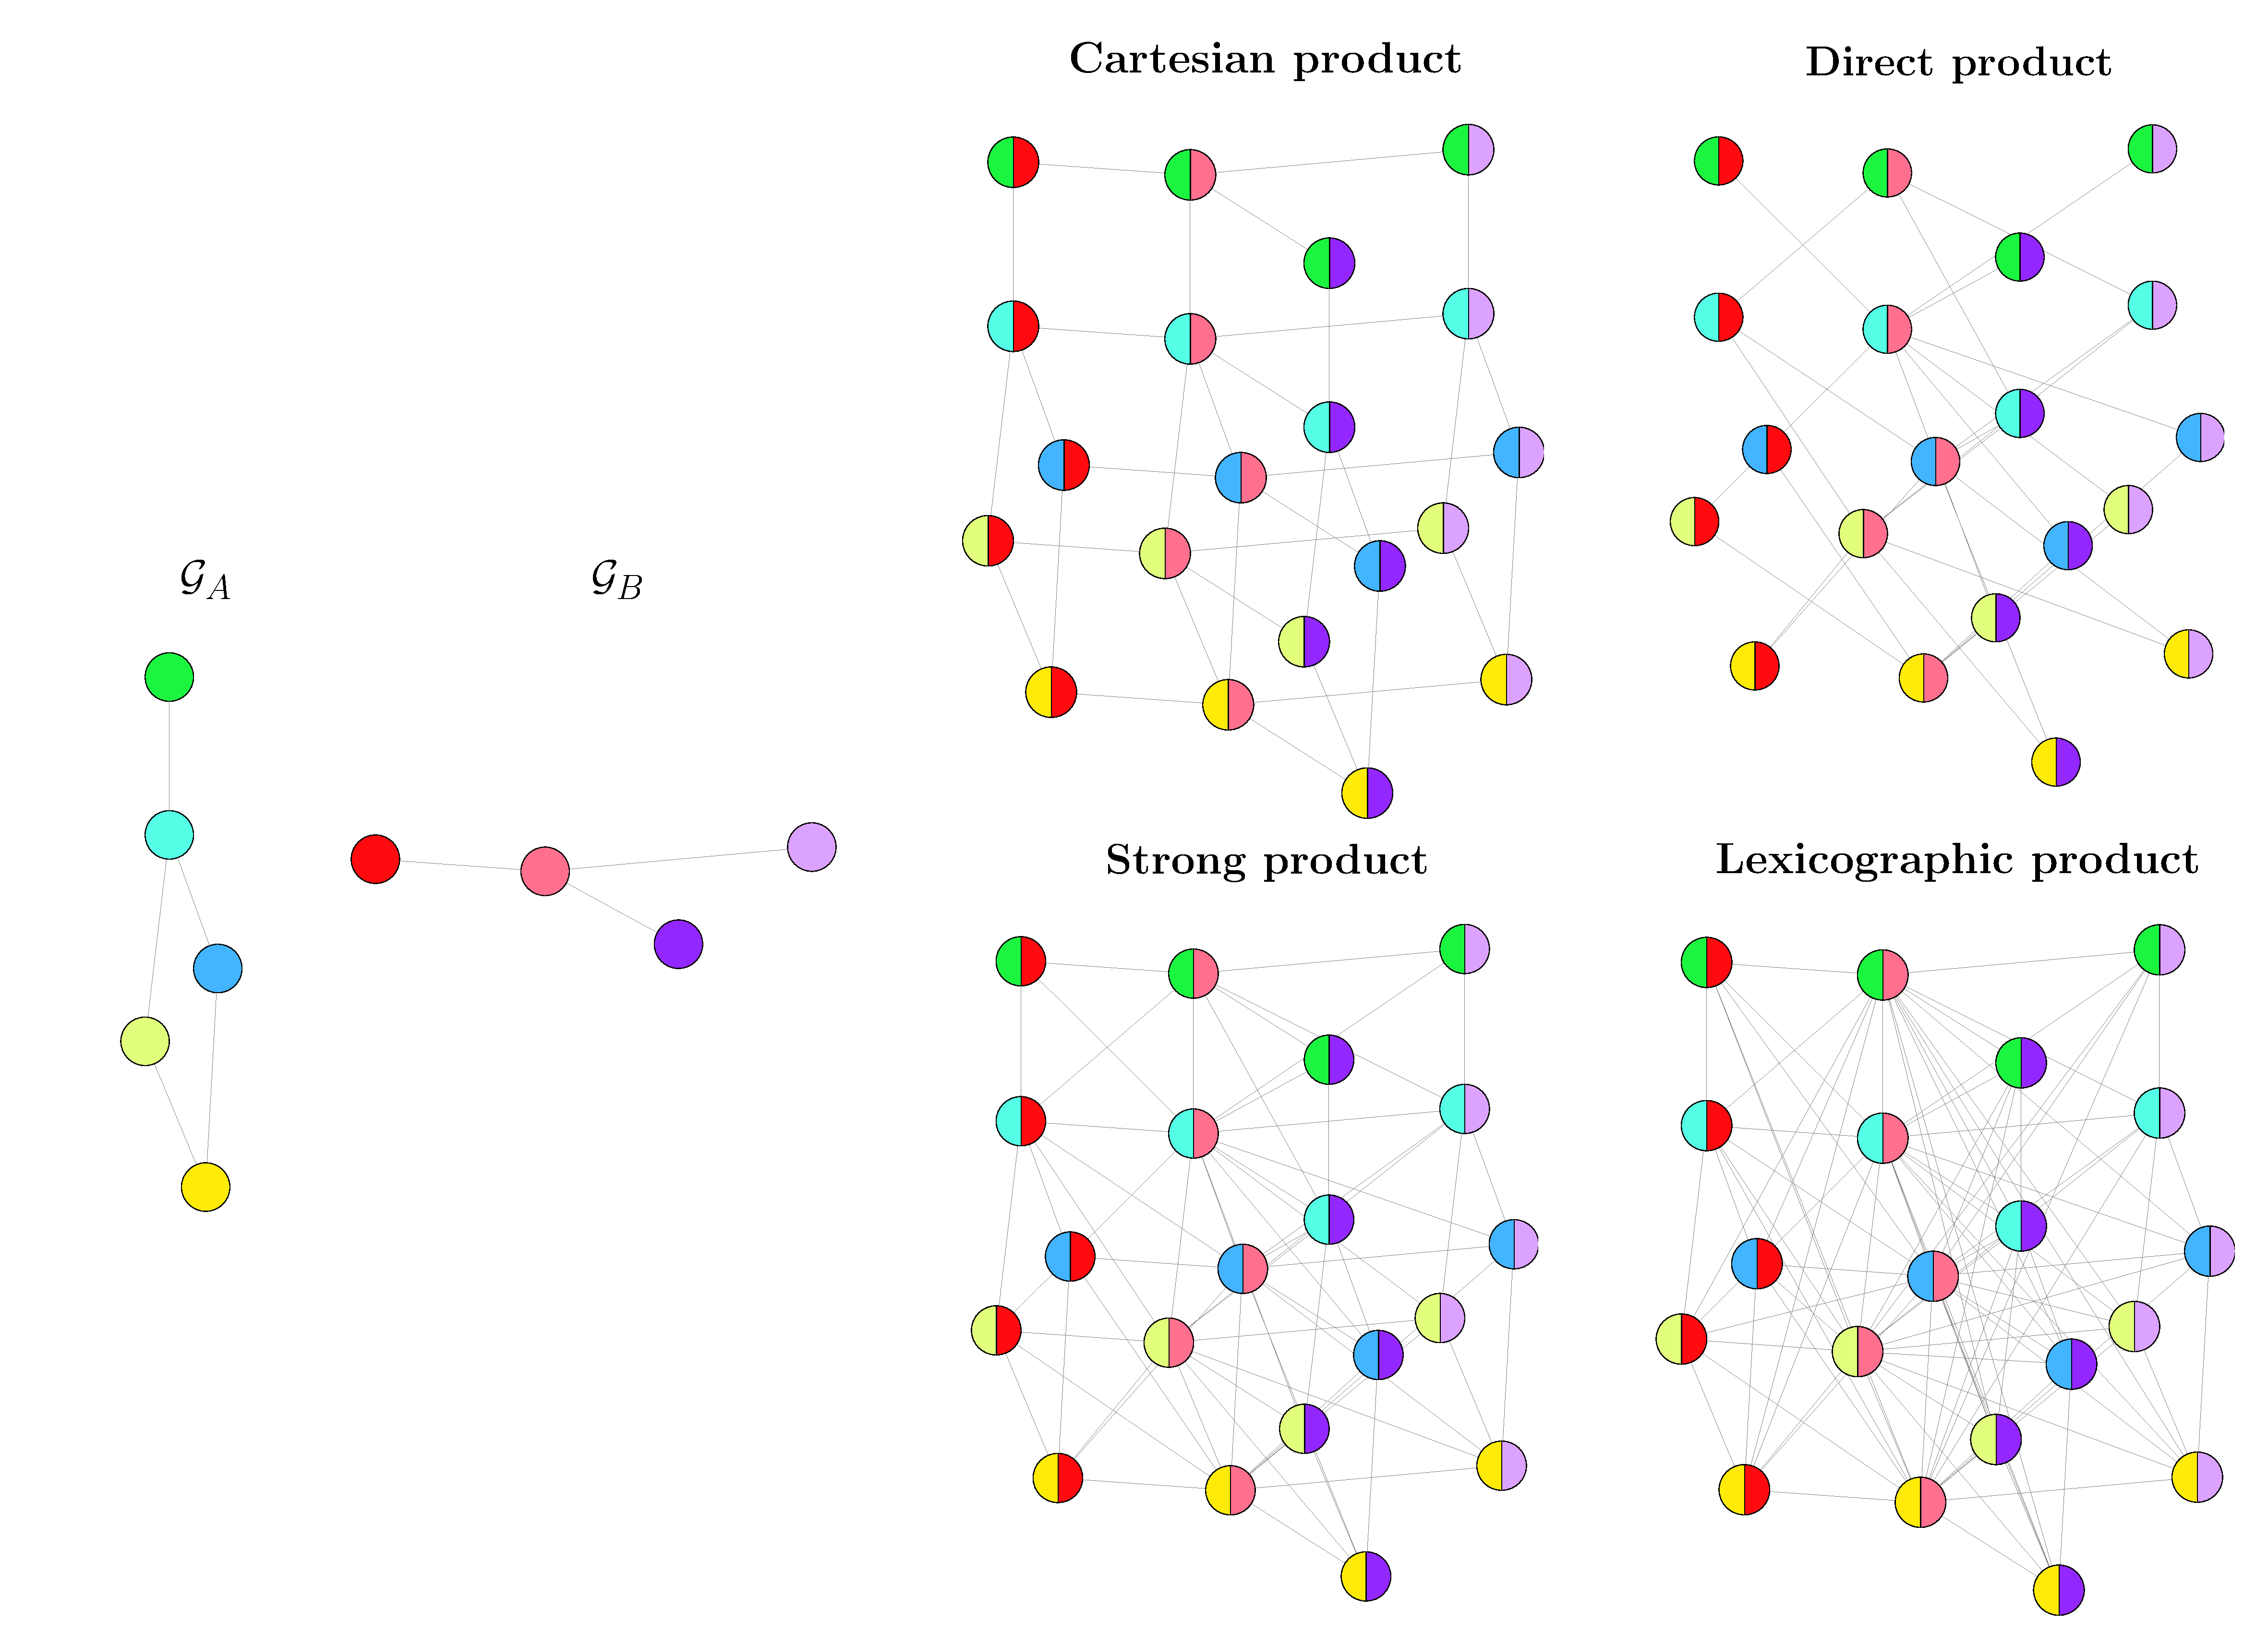
\includegraphics[width=\linewidth]{Figures/product_graphs.pdf}
    \end{center}
    \caption[Graphical depiction of the standard graph products]{A graphical depiction of the four standard graph products}
    \label{fig:graph_products}
\end{figure}

% choice of product effect the sparsity or A/cardinality of V

% What is the natural 256 ordering in terms of sparsity

% make small example in terms of vertex order

Given these definitions, it may seem that all the standard graph products are non-commutative in the sense that $\A_A \oplus \A_B  \neq \A_B \oplus \A_A $ etc. However, the graphs $\mathcal{G}_A \, \diamond \, \mathcal{G}_B$ and $\mathcal{G}_B \, \diamond \, \mathcal{G}_A$ are in fact isomorphically identical in the case of the Cartesian, direct and strong products. This is not the case for the Lexicographic product \citep{Imrich2000}.

\subsection{The spectral properties of graph products}

In the field of graph signal processing, we are often concerned with analysing the properties of graphs via eigendecomposition of the graph Laplacian \citep{Mieghem2010}. In the case of product graphs, it is greatly preferable if we are able to fully describe the spectrum of $\mathcal{G}_A \diamond \mathcal{G}_B$ in terms of the spectra of $\mathcal{G}_A$ and $\mathcal{G}_B$ alone. This is because direct decomposition of a dense $\LL$ has time-complexity $O(A^3B^3)$, whereas decomposition of the factor Laplacians individually has complexity $O(A^3 + B^3)$. As the graphs under considerations become medium to large, this fact quickly makes direct decomposition of the product graph Laplacian intractable. However, in the general case, only the spectra of the Cartesian and lexicographic graph products can be described in this way \citep{Barik2018}. In the case of the direct and strong product, it is possible to estimate the spectra without performing the full decomposition (see \citep{Sayama2016}). However, in general, the full eigendecomposition of the product graph Laplacian can only be described in terms of the factor eigendecompositions when both factor graphs are regular.


Consider the eigendecompositions of $\LL_A$ and $\LL_B$.

\begin{equation}
    \LL_A = \U_A \LAM_A \U_A^\top, \aand \LL_B = \U_B \LAM_B \U_B^\top
\end{equation}

where $\U_A$ and $\U_B$ are the respective orthonormal eigenvector matrices, and $\LAM_A$ and $\LAM_B$ are the diagonal eigenvalue matrices given by

\begin{equation}
    \LAM_A = \begin{bmatrix}
        \lambda_1^{(A)}, &                 &        &                 \\
                         & \lambda_2^{(A)} &        &                 \\
                         &                 & \ddots &                 \\
                         &                 &        & \lambda_A^{(A)} \\
    \end{bmatrix}
    \aand
    \LAM_B = \begin{bmatrix}
        \lambda_1^{(B)}, &                 &        &                 \\
                         & \lambda_2^{(B)} &        &                 \\
                         &                 & \ddots &                 \\
                         &                 &        & \lambda_B^{(B)} \\
    \end{bmatrix}
\end{equation}

Given these definitions, table \ref{tab:product_graph_spectra} gives information about the spectral decomposition of the standard graph products.

% see the effect of preconditioning matrix on different graph products 

\begin{table}[h]
    \def\arraystretch{1.8}
    \centering
    \small
    \vspace{0.5cm}
    \begin{tabular}{|l|cc|}
        \hline

         & Eigenvalues
         & Eigenvectors                                                                          \\

        \hline

        Cartesian
         & $\lambda_a^{(A)} + \lambda_b^{(B)}$
         & $(\U_A)_a \otimes (\U_B)_b$                                                           \\

        Direct$^{\star}$
         & $r_A \lambda_b^{(B)} + r_B \lambda_a^{(A)} - \lambda_a^{(A)} \lambda_b^{(B)}$
         & $(\U_A)_a \otimes (\U_B)_b$                                                           \\

        Strong$^{\star}$
         & $(1+r_A) \lambda_b^{(B)} + (1+r_B) \lambda_a ^{(A)}- \lambda_a^{(A)} \lambda_b^{(B)}$
         & $(\U_A)_a \otimes (\U_B)_b$                                                           \\

        \multirow{2}{7em}{Lexicographic$^\dagger$}
         & $B \lambda_a^{(A)}$
         & $(\U_A)_a \otimes \mathbf{1}_B$                                                       \\

         & $\lambda_b^{(B)} + B \text{deg}(a)$
         & $\mathbf{e}_a \otimes (\U_B)_b$                                                       \\

        \hline
    \end{tabular}
    \vspace{0.2cm}
    \caption[Spectral decomposition of product graphs]{Eigendecomposition of the Laplacian of the standard graph products. Here, $a$ and $b$ are understood to run from 1 to $A$ and 1 to $B$ respectively. $\star$ only for $r_A$ and $r_B$-regular factor graphs. $\dagger$ note that the $b$ runs from 2 to $B$ in the lower row. }
    \vspace{0.3cm}
    \label{tab:product_graph_spectra}
\end{table}

% remark common degree locally only necessary 
% subspace concentration 


\subsection{GSP with Cartesian product graphs}

While both the direct and strong products do find uses in certain applications (for example, see \citep{Kaveh2011}), they are both less common and more challenging to work with in a graph signal processing context due to their spectral properties described in the previous subsection. In practice, being limited to regular factor graphs means the majority of practical GSP applications are ruled out. The lexicographic product does not share this drawback, however it is also significantly less common than the Cartesian product in real-world applications. For this reason, in the following, we focus primarily on the Cartesian product.

Given the spectral decomposition of the Cartesian graph product stated in table \ref{tab:product_graph_spectra}, we can write the Laplacian eigendecomposition in matrix form as follows.

\begin{equation}
    \LL = \U \LAM \U^\top, \where \U = \U_A \otimes \U_B \aand \LAM = \LAM_A \oplus \LAM_B
\end{equation}

This motivates the following definitions for the Graph Fourier Transform (GFT) and its inverse (IGFT). Consider a signal defined over the nodes of a Cartesian product graph expressed as a matrix $\Y \in \R^{B \times A}$. We can perform the GFT as follows.

% when is this well-defined? 
% FFT version?
% impose statements on the properties of Y
% stationarity? 


\begin{equation}
    \text{GFT}(\Y) = \MAT{\big( \U_A^\top \otimes \U_B^\top \big) \, \vecc{\Y}} = \U_B^\top \Y \U_A
\end{equation}

Correspondingly, we can define the IGFT acting on a matrix of spectral components $\Z \in \R^{B \times A}$ as follows.

\begin{equation}
    \text{IGFT}(\Z) = \MAT{\big( \U_A \otimes \U_B \big)\,\vecc{\Z}} = \U_B \Z \U_A^\top
\end{equation}


\note{Product graph signals: repseprentation and vectorisation}{

    It is natural to assume that signals defined on the nodes of a Cartesian product graph $\mathcal{G}_A \, \square \; \mathcal{G}_B$ could be represented by matrices (order two tensors) of shape $(A \times B)$. Since product graph operators, such as the Laplacian $\LL_A \oplus \LL_B$, act on vectors of length $AB$, we must define a consistent function to map matrix graph signals $\in \R^{A \times B}$ to vector graph signals $\in \R^{AB}$. The standard mathematical operator for this purpose is the $\vecc{\cdot}$ function, along with its reverse operator $\mat{\cdot}$. However, this is somewhat problematic since $\vecc{\cdot}$ is defined to act in \textit{column-major} order, that is

    $$
        \text{vec} \left( \begin{bmatrix}
                \Y_{(1, 1)} & \Y_{(1, 2)} & \dots  & \Y_{(1, B)} \\
                \Y_{(2, 1)} & \Y_{(2, 2)} & \dots  & \Y_{(2, B)} \\
                \vdots      & \vdots      & \ddots & \vdots      \\
                \Y_{(A, 1)} & \Y_{(A, 2)} & \dots  & \Y_{(A, B)} \\
            \end{bmatrix} \right)
        =
        \begin{bmatrix}
            \Y_{(1, 1)} \\ \Y_{(2, 1)} \\ \vdots \\ \Y_{(A-1, B)} \\ \Y_{(A, B)}
        \end{bmatrix}
    $$

    As is visible, this does not result in a lexicographic ordering of the matrix elements when the graph signal has shape $(A \times B)$. Therefore, to avoid this issue and to be consistent with standard mathematical notation, we will assume that graph signals are represented by matrices  of shape $(B \times A)$ when considering the product between two graphs $\mathcal{G}_A \, \square \, \mathcal{G}_B$. For graph signals of this shape, the first index represents traversal of the nodes in $\mathcal{G}_B$, and the second index represents traversal of the nodes in $\mathcal{G}_A$. This ensures that matrix elements are correctly mapped to vector elements when using the column-major $\vecc{\cdot}$ function.

}

Given these definitions, we can define a spectral operator (usually a low-pass filter) $\HH$ which acts on graph signals according to a spectral scaling function $g(\lambda \,; \, \beta)$ such as one of those defined in table \ref{tab:iso_filters}. As with regular non-product graphs, the action of this operator can be understood as first transforming a signal into the Laplacian frequency domain via the GFT, then scaling the spectral components according to some function, and finally transforming back into the vertex domain via the IGFT.

\begin{align}
    \label{eq:graph_filter}
    \HH & = g(\LL_A \oplus \LL_B) \notag                                                                                          \\
        & = \big( \U_A \otimes \U_B \big) \, g \big( \LAM_A \oplus \LAM_B \big) \, \big( \U_A^\top \otimes \U_B^\top \big) \notag \\
        & = \big( \U_A \otimes \U_B \big) \, \Diag{\vecc{\G}} \, \big( \U_A^\top \otimes \U_B^\top \big)
\end{align}

% remark which section of the thesis the properties of G are explained

The matrix $\G \in \R^{B \times A}$, which we refer to as the spectral scaling matrix, holds the value of the scaling function applied to the sum of
pairs of eigenvalues, such that

\begin{equation}
    \label{eq:Gba}
    \G_{ba} = g\left(\lambda^{(A)}_a + \lambda^{(B)}_b; \beta\right)
\end{equation}


% remark about Cartesian product eig sum

We observe that defining the filtering operation in this manner implies that the intensity is equal across both $\mathcal{G}_A$ and $\mathcal{G}_B$. We refer to filters of this type as \textit{isotropic}. This can be further generalised by considering an \textit{anisotropic} graph filter, which offers independent control over the filter intensity in each of the two dimensions. In this case, we define $\G$ as follows.

\begin{equation}
    \label{eq:Gba2}
    \G_{ba} =  g \left(\lambda^{(A)}_a, \lambda^{(B)}_b; \, \beta_a, \beta_b\right)
\end{equation}

where now $g$ is chosen to be an anisotropic graph filter such as one of those listed in table \ref{tab:anis_filters_2d}. Note that the original parameter $\beta$ is now replaced by two parameters $\beta_a$ and $\beta_a$ which offer control over the filter intensity in each dimension. Filters of this kind appear often in image processing literature \citep{Aubert2006}, however, their use in graph signal processing is so far limited. \Cref{fig:filters} depicts an anisotropic graph filter applied to an image, which is a special case of a 2D Cartesian product graph signal.  


\begin{table}[t]
    \def\arraystretch{1.7}
    \small
    \begin{center}
        \begin{tabular}{|l|c|}
            \hline
            \textbf{Filter}   & $g(\lambda_a, \lambda_b; \,\beta_a, \beta_b)$                                            \\
            \hline
            1-hop random walk & $(1 + \beta_a \lambda_a + \beta_b \lambda_b)^{-1}$                                   \\
            \hline
            Diffusion         & $\exp(-\beta_a \lambda_a - \beta_b \lambda_b)$                                       \\
            \hline
            ReLu              & $\max (1 - \beta_a \lambda_a - \beta_b \lambda_b, 0)$                                \\
            \hline
            Sigmoid           & $2 \big( 1 + \exp(\beta_a \lambda_a + \beta_b \lambda_b)\big)^{-1}$                  \\
            \hline
            Bandlimited       & $1, \,\text{if} \; \beta_a \lambda_a + \beta_b \lambda_b\leq 1 \; \text{else} \; 0$ \\
            \hline
        \end{tabular}
    \end{center}
    \caption{Anisotropic graph filter functions in two dimensions}
    \label{tab:anis_filters_2d}
\end{table}


\begin{figure}[t]
    % \begin{center}
    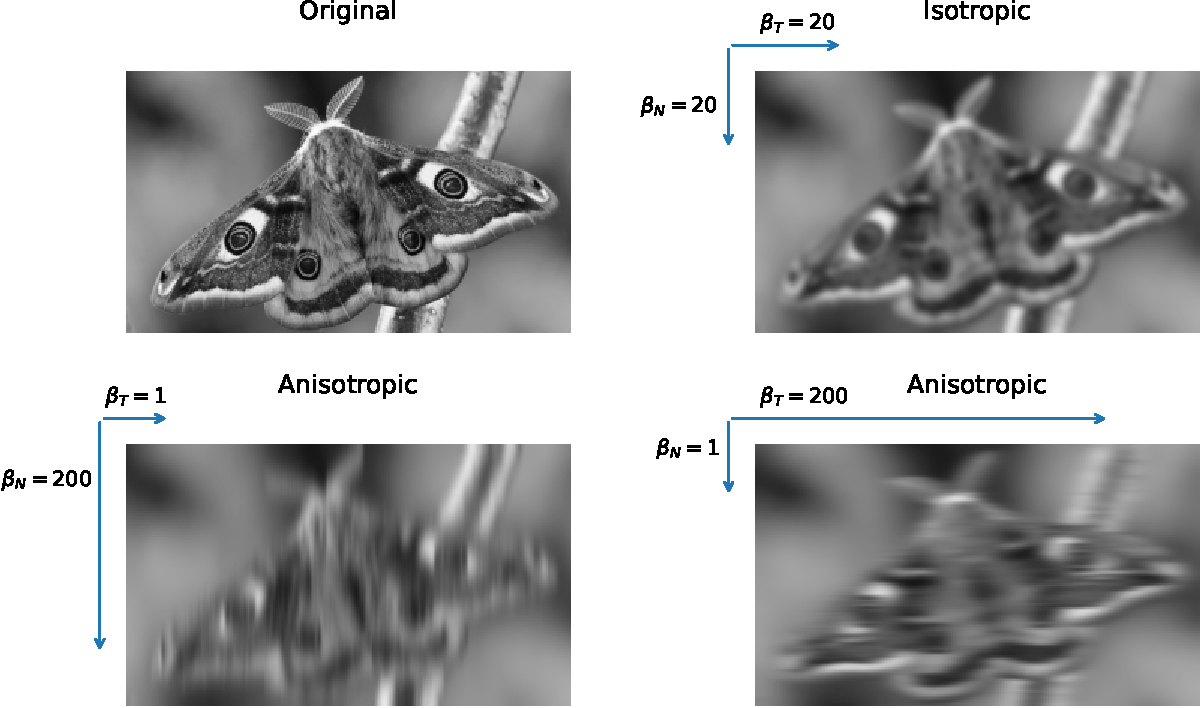
\includegraphics[width=0.9\linewidth]{Figures/filter_types_butterfly.pdf}
    % \end{center}
    \caption[A time-vertex Cartesian product graph]{A graphical depiction of a time-vertex Cartesian product graph}
    \label{fig:filters}
\end{figure}



\section{Graph Signal Reconstruction on Cartesian Product Graphs}

\label{sec:gsr_cpg}

We now turn our attention to the task of signal reconstruction on Cartesian product graphs. In the following, we will replace the factor graph labels $A$ and $B$ with $T$ and $N$ respectively. The reason for this is that one application of particular interest is graph time-series problems, where we seek to model a network of $N$ nodes across a series of $T$ discrete time points. These so called ``time-vertex'' (T-V) problems have garnered significant interest recently in the context of GSP \citep{Grassi2018, Isufi2017, Loukas2016}. T-V signals can be understood as existing on the nodes of a Cartesian product graph $\mathcal{G}_T \, \square \, \mathcal{G}_N$. In particular, we can conceptualise $T$ repeated measurements of a signal defined across the nodes of a $N$-node graph as a single measurement of a signal defined on the nodes of $\mathcal{G}_T \, \square \, \mathcal{G}_N$, where $\mathcal{G}_T$ is a simple path graph.

\vspace{1cm}


\begin{figure}[t]
    \begin{center}
        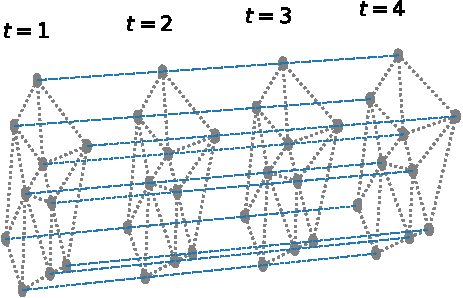
\includegraphics[width=0.5\linewidth]{Figures/T-V.pdf}
    \end{center}
    \caption[A time-vertex Cartesian product graph]{A graphical depiction of a time-vertex Cartesian product graph}
    \label{fig:TV}
\end{figure}



\note{On the Laplacian spectrum of the path graph}{
    \label{box}
    When considering time-vertex problems with uniformly spaced time intervals, $\mathcal{G}_T$ will be described by a path graph with equal weights on each edge. This special case of a graph has vertices given by $\mathcal{V}_T = \{t \in \mathbb{N} \, | \, t \leq T \}$ and edges given by $\mathcal{E}_T = \{ \, [t, t+1] \, | \, t < T \}$. The Laplacian matrix of the path graph is therefore given by

    $$
        \LL_T = \begin{bmatrix}
            1  & -1 &        &    &    \\
            -1 & 2  & -1     &    &    \\
               &    & \ddots &    &    \\
               &    & -1     & 2  & -1 \\
               &    &        & -1 & 1  \\
        \end{bmatrix}
    $$

    The eigenvalues and eigenvectors of this Laplacian are well-known and can be expressed in closed-form \citep{Jiang2012}. In particular,

    $$
        \lambda^{(T)}_t = 2 - 2 \cos \Big(  \, \frac{t - 1}{T} \pi \, \Big)
    $$

    and

    $$
        (\U_T)_{ij} = \cos \Big( \, \frac{j - 1}{T}\big(i - \frac{1}{2}\big)\pi \, \Big)
    $$

    where the columns of $\U$ are appropriately normalised such that the magnitude of each eigenvector is one. Furthermore, this implies that that the graph Fourier transform of a signal $\y \in \R^{T}$ is given by the orthogonal type-II Discrete Cosine Transform (DCT) \citep{Ahmed1974}. This is of significance, as it means we can leverage Fast Cosine Transform (FCT) algorithms \citep{Makhoul1980} which operate in a similar manner to the well-known Fast Fourier Transform (FFT) \citep{Cooley1965}. See chapter 4 of \cite{Rao1990} for an overview of FCT algorithms.

    \vspace{0.2cm}

    In particular, this reduces both of the following procedures

    \begin{equation*}
        \text{GFT}(\y) = \U^\top \y \aand \text{IGFT}(\y) = \U \y
    \end{equation*}

    from $O(T^2)$ operations to $O(T \log T)$ operations, which can be significant for large time-series problems. The figure below compares the time to compute the graph Fourier transform of a random signal using the matrix multiplication method vs the FCT implementation. In particular, we varied $T$ from 10 to 15,000 in 20 equally spaced increments, and measured the mean time to compute $\U^\top \y$ across five independent trials using both the standard matrix multiplication and the Fast Cosine Transform method. As is visible, the difference becomes extremely pronounced as $T$ grows large.

    % \begin{figure}[h]
    \begin{center}
        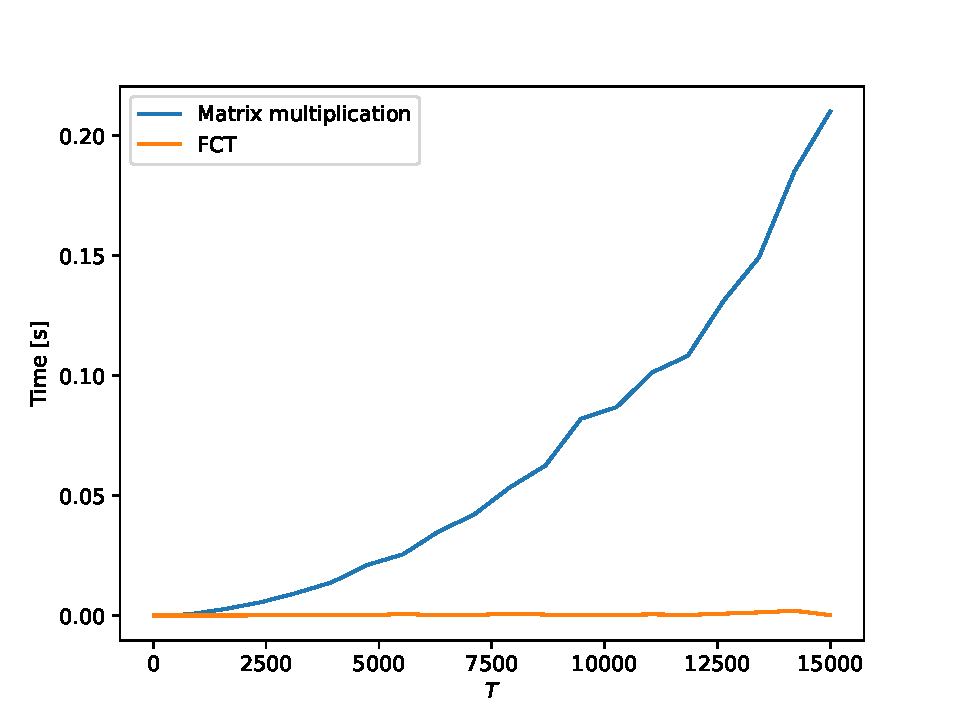
\includegraphics[width=\linewidth]{Figures/DCT.pdf}
    \end{center}
    % \caption[Run time comparison for DCT]{A graphical depiction of the four standard graph products}
    % \label{fig:DCT}
    % \end{figure} 

    % write algorithm explicitly
    % what is aliasing in this context? 
    % Nyquist for GFT? 


}



Note that, despite the observation that $\mathcal{G}_T$ is often a path graph in the context of T-V problems, the methods introduced in this section are valid for the Cartesian product between arbitrary undirected factor graphs.

\subsection{Problem statement}

\label{sec:problem_statement_2d}


The goal of Graph Signal Reconstruction (GSR) is to estimate the value of a partially observed graph signal at nodes where no data was collected. In the context of GSR on a Cartesian product graph, the available data is an observed signal $\Y \in \R^{N \times T}$ where only a partial set $\mathcal{S} = \{(n_1, t_1), (n_2, t_2), \dots \}$ of the signal elements were recorded. All other missing elements of $\Y$ are set to zero. Our model is based on the assumption that $\Y$ is a noisy partial observation of an underlying signal $\F \in \R^{N \times T}$, which is itself assumed to be smooth with respect to the graph topology.

We define the statistical model for the generation of an observation matrix $\Y$ as follows. 

\begin{equation}
    \Y = \Ss \circ \big(\F + \E \big)
\end{equation}

where $\Ss \in [0, 1]^{N \times T}$ is referred to as the sensing matrix, and has entries given by

\begin{equation}
    \Ss_{nt} = \begin{cases}
        1 & \text{if} \;\; (n, t) \in \mathcal{S} \\
        0 & \text{otherwise}
    \end{cases}
\end{equation}

The matrix $\E$ represents the model error and is assumed to have an independent normal distribution with unit variance. Therefore, the probability distribution of $\Y$ given the latent signal $\F$ is

\begin{equation}
    \label{eq:Y_given_F}
    \vecc{\Y} \, | \, \F \sim \mathcal{N}\Big(\vecc{\Ss \circ \F}, \; \Diag{\vecc{\Ss}}\Big)
\end{equation}

Note that the covariance matrix $\Diag{\vecc{\Ss}}$ is semi-positive definite by construction. This naturally reflects the constraint that some elements of $\Y$ are zero with probability 1. In order to estimate the latent signal $\F$, we must provide a prior distribution describing our belief about its likely profile ahead of time. In general, we expect $\F$ to be smooth with respect to the topology of the graph. This can be expressed by setting the covariance matrix in its prior to be proportional to $\HH^2$, where $\HH$ is a graph filter as defined in equation (\ref{eq:graph_filter}). For now, in the absence of any further information, we assume that the prior mean for $\F$ is zero across all elements.

\begin{equation}
    \label{eq:F_prior}
    \vecc{\F} \sim \mathcal{N}\big(\mathbf{0}, \, \gamma^{-1} \HH^2\big)
\end{equation}

Next, given an observation $\Y$, we use Bayes' rule to find the posterior distribution over $\F$. This is given by

\begin{equation}
    \pi\big(\vecc{\F} \, | \, \Y \big) = \frac{\pi\big(\vecc{\Y} \, | \, \F \big) \pi(\F) }{\pi(\Y)}.
\end{equation}

where we use the notation $\pi(\cdot)$ to denote a probability density function.

The posterior distribution for $\F$ is given by

\begin{equation}
    \label{eq:F_post}
    \Vecc{\F} \, | \, \Y \sim \mathcal{N} \big(\SIG \, \Vecc{\Y}, \; \SIG \big)
\end{equation}

\noindent where

\begin{equation}
    \label{eq:Sig_post}
    \SIG = \Big(\Diag{\vecc{\Ss}} + \gamma  \HH^{-2}\Big)^{-1}
\end{equation}

A proof of this can be found in the appendix, theorem \ref{the:F_posterior}.



In this chapter, we are primarily interested in computing the posterior mean, which is the solution to the following linear system.

\begin{equation}
    \label{eq:lin_system}
    \vecc{\F} = \Big(\Diag{\vecc{\Ss}} + \gamma  \HH^{-2}\Big)^{-1} \vecc{\Y}
\end{equation}

We return to the question of sampling from the posterior and estimating the posterior covariance directly in \cref{chap:variance}.

Two significant computational challenges arise when working with non-trivial graph signal reconstruction problems, where the number of vertices in the product graph is large. First, although the posterior mean point estimator given in \cref{eq:lin_system} has an exact closed-form solution, its evaluation requires solving an $NT \times NT$ system of equations, which is impractical for all but the smallest of problems. Second, since the eigenvalues of $\HH$ can be close to or exactly zero, $\HH^{-2}$ may be severely ill-conditioned and even undefined. This means the condition number of the coefficient matrix may not be finite, making basic iterative methods to numerically solve the linear system, such as steepest descent, slow or impossible. The models proposed in this paper aim to overcome these problems.


Since the coefficient matrix defining the system is of size $NT \times NT $, direct methods such as Gaussian elimination are assumed to be out of the question. In such cases, one often resorts to one of three possible solution approaches: stationary iterative methods; Krylov methods; and multigrid methods. Each are part of the family of iterative methods which are most commonly found in applications of sparse matrices, such as finite element methods \citep{Brenner2008}. In the following, we propose a stationary iterative method and a Krylov method and compare their relative behaviour. In both cases, we show that each step of the iterative process can be completed in $O(N^2T + NT^2)$ operations, making a solution feasible for relatively large graph problems. First, we present each of the methods in isolation. Then, the convergence behaviour of each is derived theoretically and verified numerically.


\subsection{A stationary iterative method}

\label{sec:SIM}

In this section, we demonstrate a technique for obtaining the posterior mean by adopting a classic approach to solving linear systems, known as \textit{matrix splitting}, which sits within the family of Stationary Iterative Methods (SIMs) \citep{Saad2003}. The general splitting strategy is to break the coefficient matrix into the form $\M - \N$, such that 


\begin{equation}
    \vecc{\F} = (\M - \N)^{-1} \vecc{\Y}
\end{equation}

By noting that

\begin{align}
    \M \vecc{\F} &= \N \vecc{\F} + \vecc{\Y} \\
    \vecc{\F} &= \M^{-1}\N \vecc{\F} + \M^{-1} \vecc{\Y}
\end{align}

we devise an iterative scheme given by 

\begin{equation}
    \label{eq:sim_update}
    \vecc{\F_{k+1}} = \M^{-1}\N \vecc{\F_{k}} + \M^{-1} \vecc{\Y}
\end{equation}


When $\M$ is a simple matrix that is easy to invert, this update function can be vastly more efficient to compute. Common approaches to finding a suitable value for $\M$ and $\N$ include the Jacobi, Gauss-Seidel and successive over-relaxation methods, each of which represent a different strategy for splitting the coefficient matrix \citep{Saad2003}. However, whilst these techniques are well-studied, they are not appropriate for use in the case of graph signal reconstruction. This is because, for each of these methods, the coefficient matrix is split according to its diagonal and off-diagonal elements in some way. Consequently, this would require the evaluation of $\HH^{-2}$ directly which, as we have discussed, may be large, severely ill-conditioned and possibly ill-defined. 


Instead, we require a custom splitting that avoids direct evaluation of $\HH^{-2}$, and allows the right hand side of \cref{eq:sim_update} to be computed efficiently. The main contribution of this subsection is the identification of appropriate values for $\M$ and $\N$, and an investigation of the consequences of that choice. 

In the folowing, we set 

\begin{equation}
    \M = \gamma \HH^{-2} + \I_{NT}, \aand \N = \Diag{\vecc{\Ss'}}.
\end{equation}

where $\Ss'$ is the binary matrix representing the complement of the set of selected nodes, i.e.

\begin{equation}
    \label{eq:S_}
    \Ss'_{nt} = \begin{cases}
        1 & \text{if} \;\; (n, t) \notin \mathcal{S} \\
        0 & \text{otherwise}
    \end{cases}
\end{equation}

In this way, the update equation is given by 

\begin{equation}
    \label{eq:sim_update2}
    \vecc{\F_{k+1}} = \big(\gamma \HH^{-2} + \I \, \big)^{-1}  \Diag{\vecc{\Ss'}} \vecc{\F_{k}} + \big(\gamma \HH^{-2} + \I \, \big)^{-1} \vecc{\Y}
\end{equation}



Note that this splitting is valid since $\big(\gamma\HH^{-2} + \I \, \big)^{-1}$ is guaranteed to exist. It can also be readily computed as we already have the eigendecomposition of $\HH$. Noting the decomposed definition of $\HH$ given in \cref{eq:graph_filter}, this can be written as

\begin{align}
    \label{eq:inv}
    \M^{-1} & = \Big( \gamma \HH^{-2} + \I \, \Big)^{-1} \notag \\
            & = \Big( \gamma \big(\U_T \otimes \U_N\big)\, \Diag{\vecc{\G}}^{-2}\,  \big(\U_T^\top \otimes \U_N^\top\big)  + \I \, \Big)^{-1} \notag   \\
            & = \big(\U_T \otimes \U_N\big)\, \Big( \gamma \, \Diag{\vecc{\G}}^{-2}\,    + \I \, \Big)^{-1} \big(\U_T^\top \otimes \U_N^\top\big) \notag \\
            & = \big(\U_T \otimes \U_N\big)\, \Diag{\vecc{\J}}\,  \big(\U_T^\top \otimes \U_N^\top\big)
\end{align}

\noindent where $\J \in \R^{N \times T}$ has elements defined by

\begin{equation}
    \label{eq:Jnt}
    \J_{nt} = \frac{\G_{nt}^2}{\G_{nt}^2 + \gamma}.
\end{equation}

Note that the update formula can be computed with $O(N^2T + NT^2)$ complexity at each step.  


\begin{align}
    \label{eq:update3}
    \F_{k+1} & = \U_N \, \big( \J  \circ \big( \U_N^\top \, (\Ss' \circ \F_{k})\, \U_T \big) \big) \, \U_T^\top + \F_0 \\
    \label{eq:update4}
    \text{with} \quad\quad\quad \F_0 & = \U_N \, \big( \J  \circ \big( \U_N^\top \, \Y \, \U_T \big) \big) \, \U_T^\top 
\end{align}


Furthermore, this is reduced to $O(N^2T + NT \log T)$ in the case of T-V problems, and to $O\big(NT \log NT \big)$ for data residing on a grid (see \cref{box}). 


It is well-know that a given splitting will be convergent if the largest eigenvalue $\lambda_{\text{max}}$ of the matrix $\M^{-1}\N$ has an absolute value of less than one. This attribute, $\rho = |\lambda_{\text{max}}|$, is known as the spectral radius. 

Whilst the spectral radius of $\M^{-1}\N$ cannot be computed directly, we can derive an upper bound based on the properties of $\M$ and $\N$ individually. 

Consider the spectral radius of $\M^{-1}$. By directly inspecting \cref{eq:inv}, it is clear that $\rho(\M^{-1})$ will be the maximum entry in the matrix $\J$ since $\M^{-1}$ is already diagonalised in the basis $\U_T \otimes \U_N$. Consider now the definition of $\J$ given in \cref{eq:Jnt}. By definition, $g(\cdot)$ has a maximum value of one on the non-negative reals, achieved when its argument is zero. Since the graph Laplacian is guaranteed to have at least one zero eigenvalue, the maximum entry in the matrix $\J$, and therefore the spectral radius of $\M^{-1}$, is surely given by

\begin{equation}
    \rho(\M^{-1}) = \frac{1}{1 + \gamma}
\end{equation}

Next, consider the spectral radius of $\N$. This can be extracted directly as 1, since it is a diagonal binary matrix. Since both $\M^{-1}$ and $\N$ are positive semi-definite, we can apply the theorem

\begin{equation}
    \label{eq:psd}
    \rho(\A\B) \leq \rho(\A) \, \rho(\B)
\end{equation}

\citep{Bhatia1997}. Therefore, the spectral radius of $\M^{-1}\N$ is guaranteed to be less than or equal to $1 / (1 + \gamma)$.  Since $\gamma$ is strictly positive, this is less than one and, as such, convergence is guaranteed. We return to the question of convergence more thoroughly in \cref{sec:SIM_convergence}. 

Finally, the update formulas given in \cref{eq:update3,eq:update4} can be written equivalently as 

\begin{align}
    \Delta \F_0     & = \U_N \, \big( \J  \circ \big( \U_N^\top \, \Y \, \U_T \big) \big) \, \U_T^\top \notag                 \\
    \Delta \F_{k+1} & = \U_N \, \big( \J  \circ \big( \U_N^\top \, (\Ss' \circ \Delta \F_{k})\, \U_T \big) \big) \, \U_T^\top
\end{align}

In this form, the iterations can be easily terminated when $|\Delta \F_{k}|$ is sufficiently small. The complete procedure is given in \hyperlink{al1}{\textbf{algorithm 1}}.

\begin{algorithm}[t]
    \hypertarget{al1}{}
    \caption{Stationary iterative method with matrix splitting}
    \begin{algorithmic}
        \vspace{0.05cm}
        \Require{Observation matrix $\Y \in \R^{N \times T}$}
        \vspace{0.05cm}
        \Require{Sensing matrix $\Ss \in [0, 1]^{N \times T}$}
        \vspace{0.05cm}
        \Require{Space-like graph Laplacian $\LL_N \in \R^{N \times N}$}
        \vspace{0.05cm}
        \Require{Time-like graph Laplacian $\LL_T \in \R^{T \times T}$}
        \vspace{0.05cm}
        \Require{Regularisation parameter $\gamma \in \R^{+}$}
        \vspace{0.05cm}
        \Require{Graph filter function $g(\, \cdot\, \,; \betaa \in \R^{2})$}
        \vspace{0.15cm}
        \State{Decompose $\LL_N$ into $\U_N \LAM_L \U_N^\top$ and $\LL_T$ into $\U_T \LAM_T \U_T^\top$}
        \vspace{0.15cm}
        \State{Compute $\G \in \R^{N \times T}$ as $\G_{nt} = g \left(\lambda^{(A)}_a, \lambda^{(B)}_b; \, \beta_a, \beta_b\right)$ }
        \vspace{0.15cm}
        \State{Compute $\J \in \R^{N \times T}$ as $\J_{nt} = \G_{nt}^2 / (\G_{nt}^2 + \gamma)$ }
        \vspace{0.15cm}
        \State{$\Ss' \leftarrow \mathbf{1} \in \R^{N \times T} - \Ss$}
        \vspace{0.15cm}
        \State{$\Delta\F \leftarrow \U_N\big( \J \circ (\U_N^\top \Y \U_T) \big)\U_T^\top$}
        \vspace{0.15cm}
        \State{$ \F  \leftarrow \Delta\F$}
        \vspace{0.15cm}
        \While{$|\Delta\F| > \text{tol}$}
        \vspace{0.15cm}
        \State{$\Delta\F \leftarrow \U_N \Big( \J \circ \big( \U_N^\top\, (\Ss' \circ \Delta\F ) \, \U_T \big) \Big) \U_T^\top$}
        \vspace{0.15cm}
        \State{$ \F \leftarrow  \F  + \Delta\F$}
        \vspace{0.15cm}
        \EndWhile
        \vspace{0.15cm}
        \Ensure{$ \F $}
        \vspace{0.15cm}
        \label{al:SIM}
    \end{algorithmic}
\end{algorithm}

\subsection{A conjugate gradient method}

The second approach we consider for computing the posterior mean is to use the Conjugate Gradient Method (CGM). First proposed in 1952, the CGM is part of the Krylov subspace family, and is perhaps the most prominent iterative algorithm for solving linear systems \citep{Hestenes1952}. In computational terms, the method only requires repeated forward multiplication of vectors by the coefficient matrix which, in the standard CGM, bust be PSD. It is therefore effective in applications where this process can be performed efficiently. 

In brief, the CGM seeks to solve the linear system $\A \x = \bb$ by minimising, at the $k$-th iteration, some measure of error in the affine space $\x_0 + \mathcal{K}_k$ where $\mathcal{K}_k$ is the $k$-th Krylov subspace given by  

$$
\mathcal{K}_k = \text{span}\big(\rr_0, \; \A \rr_0, \, ..., \, \A^{k-1} \rr_0 \big)
$$

The residual $\rr_k$ is given by 

$$
\rr_k = \bb - \A \x
$$

and the $k$-th iterate of the CGM minimises 

$$
\phi(\x) = \frac{1}{2} \x^\top \A \x  - \x^\top \bb
$$

over $\x_0 + \mathcal{K}_k$ \citep{Kelley1995}. 

The CGM works best when the coefficient matrix $\A$ has a low condition number $\kappa$ (that is, the ratio between the largest and smallest eigenvalue is small) and, as such, a preconditioning step is often necessary. The purpose of a preconditioner is to reduce $\kappa$ by solving an equivalent transformed problem. This can be achieved by right or left multiplying the linear system by a preconditioning matrix $\PHI$. However, this likely means the coefficient matrix is no longer PSD, meaning the CGM cannot be used in its basic form. (Other approaches modified for non-PSD matrices exists, e.g. the CGNE or GIMRES \citep{Elman1982, Saad1986}). A preconditioner can also multiply the coefficient matrix on the right by a preconditioner $\PHI^\top$ and the left by $\PHI$. This preserves the symmetry meaning we can can continued to use the regular CGM. 

In our case, where the coefficient matrix is given by $\Big(\Diag{\vecc{\Ss}} + \gamma  \HH^{-2}\Big)$, preconditioning will be essential for convergence. To see why, consider the definition of $\HH$ in equation (\ref{eq:graph_filter}). A low-pass filter function $g(\cdot)$ may be close to zero when applied to the  high-Laplacian frequency eigenvalues of the graph Laplacian, meaning elements of $\Diag{\vecc{\G}}^{-2}$ may be very high. In the worst case, for example with a band-limited filter, the matrix $\HH$ will be singular, no matrix $\HH^{-2}$ will exist, and the condition number of the coefficient matrix will be, in effect, infinite. Therefore, the primary purpose of this subsection is to find a preconditioner that maintains efficient forward multiplication and is effective at reducing the condition number of the coefficient matrix.

References such as \citep{Saad2003} give a broad overview of the known approaches to finding a preconditioner. Standard examples include the Jacobi preconditioner which is given by the inverse of the coefficient matrix diagonal and is effective for diagonally dominant matrices, and the Sparse Approximate Inverse preconditioner \citep{Grote1997}. However, such preconditioners generally require direct evaluation of parts of the coefficient matrix or are computationally intensive to calculate.

In the following, we derive an effective symmetric preconditioner that allows forward multiplication of the coefficient matrix to be performed efficiently. First consider the transformed variable $\Z$, related to $\F$ in the following way.

\begin{equation}
    \label{eq:Z_transform}
    \F = \U_N \, (\G \circ \Z) \, \U_T^\top
\end{equation}

Here, $\Z$ can be interpreted as set of Laplacian frequency coefficients, which are subsequently scaled according to the graph filter function, and then reverse Fourier transformed back into the node domain. Matrices $\Z$ which are distributed according to a spherically symmetric distribution, result in signals $\F$ which are smooth with respect to the graph topology. Since this transform filters out the problematic high-Laplacian frequency Fourier components, the system defined by this transformed variable $\Z$ is naturally far better conditioned.

By substituting this expression for $\F$ back into the likelihood in equation (\ref{eq:Y_given_F}), and the prior of equation (\ref{eq:F_prior}), one can derive a new expression for the posterior mean of $\Z$. This is done explicitly in \cref{the:Z_transform_bayes}. The end result is that the new linear system for the transformed variable $\Z$ is given by


\begin{equation}
    \label{eq:Z_post}
    \vecc{\Z} = \big( \C + \gamma \I_T \otimes \I_N \big) ^{-1} \Vecc{\G \circ (\U_N^\top \Y \U_T)}
\end{equation}

\noindent where $\C$ is the symmetric PSD matrix


\begin{equation}
    \label{eq:Q}
    \C = \D_{\G} \, \big(\U_T^\top \otimes \U_N^\top \big)\, \D_{\Ss} \, \big(\U_T \otimes \U_N \big) \,\D_{\G}
\end{equation}

\noindent where we have abbreviated $\Diag{\vecc{\G}}$ and $\Diag{\vecc{\Ss}}$ as $\D_{\G}$ and $\D_{\Ss}$ respectively. Note that the conditioning of the coefficient matrix $\C + \gamma \I$ is greatly improved from the untransformed problem, as we will discuss in greater detail in \cref{sec:convergence}. Note also that multiplication of a vector $\vecc{\RR}$ by the coefficient matrix can be computed efficiently as 

$$
\MAT{\big(\C + \gamma \I \big)\vecc{\RR}} = \gamma \RR + \G \circ \Bigg(\U_N^\top \Big( \Ss \circ \big(\U_N (\G \circ \RR) \U_T^\top \big) \Big) \U_T\Bigg) 
$$

This has $O(N^2T + NT^2)$ complexity at each step which may be  reduced to $O(N^2T + NT \log T)$ in the case of T-V problems, and to $O\big(NT \log NT \big)$ for data residing on a grid (see \cref{box}). 

The linear system defined \cref{eq:Z_post} can be understood as a two-sided symmetrically preconditioned version of the original linear system given in \cref{eq:lin_system}. In particular, the new expression can be constructed by modifying the original system in the following way.

\begin{equation}
    \Big(\PHI^\top  \big(\D_{\Ss} + \gamma  \HH^{-2}\big) \, \PHI  \Big) \Big(\PHI^{-1}\, \vecc{ \F } \Big) = \PHI^\top \, \vecc{\Y},
\end{equation}

\noindent where

\begin{equation}
    \PHI =   \big(\U_T \otimes \U_N\big) \, \D_{\G}.
\end{equation}

Since preconditioning of the coefficient matrix on the left is achieved with $\PHI^\top$ and on the right with $\PHI$, symmetry is preserved. This ensures that one can continue to utilise algorithms tailored to work with PSD matrices. In \hyperlink{al2}{\textbf{algorithm 2}}, we outline a conjugate gradient method based on this new formulation. 

\begin{algorithm}[t]
    \hypertarget{al2}{}
    \label{al:MVGKR}
    \caption{Conjugate gradient method with graph-spectral preconditioner}
    \begin{algorithmic}
        \vspace{0.15cm}
        \Require{Observation matrix $\Y \in \R^{N \times T}$}
        \vspace{0.05cm}
        \Require{Sensing matrix $\Ss \in [0, 1]^{N \times T}$}
        \vspace{0.05cm}
        \Require{Space-like graph Laplacian $\LL_N \in \R^{N \times N}$}
        \vspace{0.05cm}
        \Require{Time-like graph Laplacian $\LL_T \in \R^{T \times T}$}
        \vspace{0.05cm}
        \Require{Regularisation parameter $\gamma \in \R$}
        \vspace{0.05cm}
        \Require{Graph filter function $g(\, \cdot\, \,; \betaa)$}
        \vspace{0.25cm}
        \State{Decompose $\LL_N$ into $\U_N \LAM_L \U_N^\top$ and $\LL_T$ into $\U_T \LAM_T \U_T^\top$}
        \vspace{0.15cm}
        \State{Compute $\G \in \R^{N \times T}$ as $\G_{nt} = g \left(\lambda^{(A)}_a, \lambda^{(B)}_b; \, \beta_a, \beta_b\right)$ }
        \vspace{0.15cm}
        \State{Initialise $\Z \in \R^{N \times T}$ randomly}
        \vspace{0.15cm}
        \State{$\RR \leftarrow \G \circ (\U_N^\top \Y \U_T) - \gamma \Z - \G \circ \Big( \, \U_N^\top \big(\Ss \circ (\U_N \, (\G \circ \Z) \, \U_T^\top) \big)  \, \U_T\Big)$}
        \vspace{0.15cm}
        \State{$\D \leftarrow \RR$}
        \vspace{0.15cm}
        \While{$|\Delta\RR| > \text{tol}$}
        \vspace{0.15cm}
        \State{$\A_D \leftarrow \gamma \D + \G \circ \Big( \, \U_N^\top \big(\Ss \circ (\U_N \, (\G \circ \D) \, \U_T^\top) \big)\, \U_T\Big) $}
        \vspace{0.15cm}
        \State{$\alpha \leftarrow  \tr{\RR^\top \RR} \, / \, \tr{\RR^\top \A_D \RR}$}
        \vspace{0.15cm}
        \State{$\Z \leftarrow  \Z + \alpha \D $}
        \vspace{0.15cm}
        \State{$\RR \leftarrow  \RR - \alpha \A_D $}
        \vspace{0.15cm}
        \State{$\delta \leftarrow \tr{\RR^\top \RR} \, / \, \tr{(\RR + \alpha \A_D)^\top (\RR + \alpha \A_D)}$}
        \vspace{0.15cm}
        \State{$\D \leftarrow  \RR + \delta \D $}
        \vspace{0.15cm}
        \EndWhile
        \vspace{0.25cm}
        \Ensure{$\U_N \, (\G \circ \Z) \, \U_T^\top$}
        \vspace{0.15cm}
    \end{algorithmic}
\end{algorithm}

\subsection{Verifying basic properties}

In this subsection, we seek to verify several basic properties of the CGM and SIM. First, we want to show that both methods converge to the same prediction for the smooth underlying signal $\F$ an check that the solution is 


\begin{figure}[t]
    \hypertarget{butterflies}{}
    \label{fig:butterflies}
    \begin{center}
        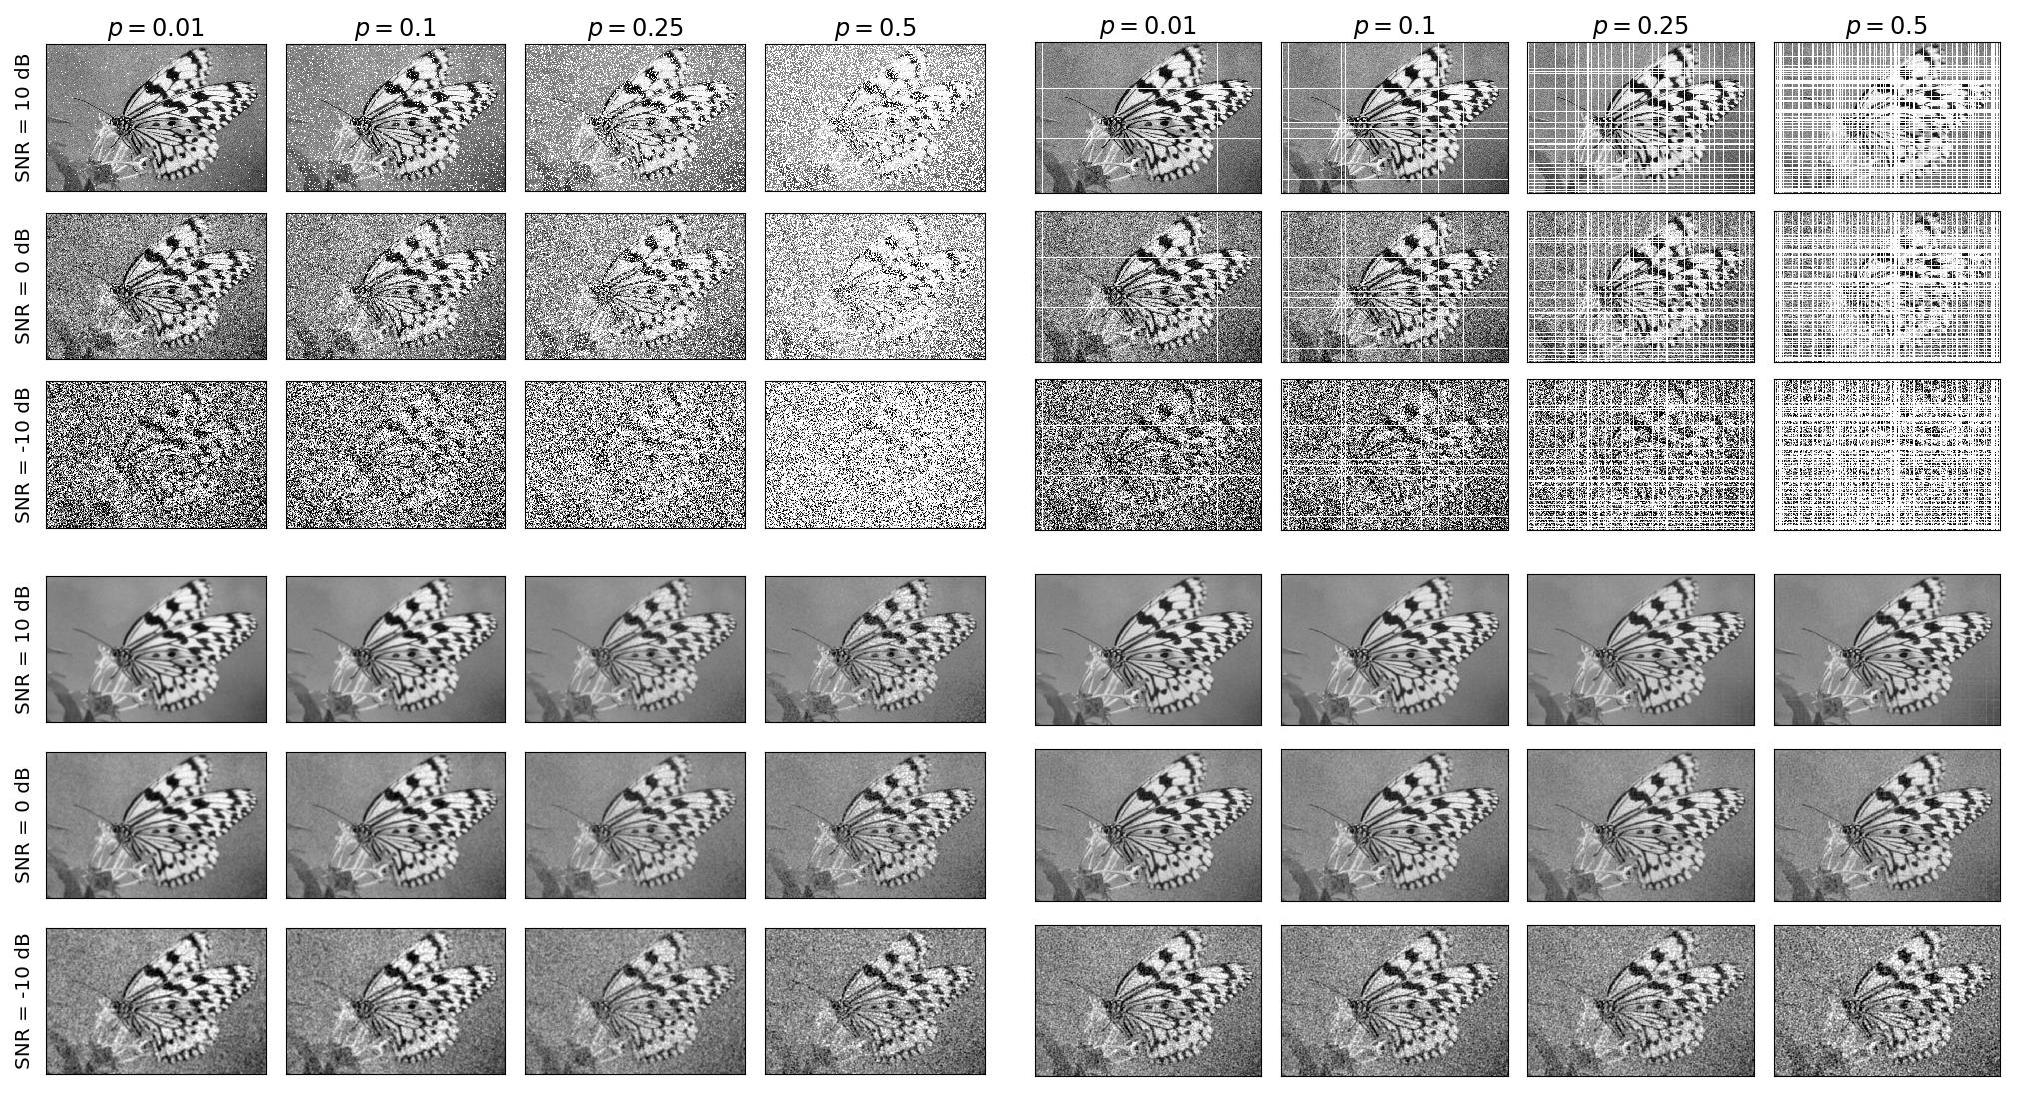
\includegraphics[width=0.95\linewidth]{Figures/butterflies.jpg}
        % \includegraphics[width=0.9\linewidth]{images/outputs.jpg}
    \end{center}
    \caption{\small{The output from the first experiment is depicted. In the top left quadrant, the input images are shown across a range of noise levels and missing pixel percentages, with missing pixels chosen uniformly at random. Below that, in the lower left quadrant, the corresponding reconstructed images are shown. The right half of the plot is the same, except here entire columns and rows of pixels are removed at random.}}
\end{figure}


\section{Convergence properties}

\label{sec:convergence}


In this section, we take a closer look at the convergence properties of both the SIM and the CGM. As we will show, the method with the best convergence rate depends on the value of the hyperparameters $\beta$, which describes the strength of the graph filter, $\gamma$, which determines the regularisation strength, and $m=|\mathcal{S}'|/NT$, which is the fraction of values that are missing from the original graph signal. For both methods, we provide bounds on the convergence rate and show how each of these three parameters can be expected to effect convergence in practice. 

We begin first with a brief review the generic convergence properties of the SIM and CGM. Next, we analyse their behaviour in the specific case of graph signal reconstruction as described in our model. We demonstrate that, for both models, the convergence rate is bounded by two edge cases; one in the limit of a weak graph filter and the other in the limit of a strong graph filter. Furthermore we show that in the weak filter limit, where $\beta \rightarrow 0$, the CGM has better convergence behaviour. On the other hand, in the strong filter limit where $\beta \rightarrow \infty$, the SIM has better convergence behaviour. We also provide intuition for selecting a method for intermediate values of $\beta$. 


\subsection{Convergence of the SIM}
\label{sec:SIM_convergence}

In the SIM, we have that 

\begin{equation}
    \label{eq:SIM_F_true}
\M \vecc{\F} =  \N \vecc{\F} + \vecc{\Y}
\end{equation}

where $\vecc{\F}$ represents the true solution to the linear system. This leads directly to an update equation given by

\begin{equation}
    \label{eq:SIM_F_update}
\M \vecc{\F_k} = \N \vecc{\F_{k-1}} + \vecc{\Y}
\end{equation}

Subtracting \cref{eq:SIM_F_true} from \cref{eq:SIM_F_update} gives

\begin{align}
    \M \vecc{\F_k} - \M \vecc{\F} &= \N \vecc{\F_{k-1}} - \N \vecc{\F}  \notag \\
    \vecc{\E_k} &= \M^{-1} \N \vecc{\E_{k-1}} \notag \\
     &= \big( \M^{-1} \N \big)^{k} \vecc{\E_{0}}
\end{align}

where we denote the error at the $k$-th iteration as $\vecc{\E_k} = \vecc{\F_k} - \vecc{\F}$. From this it is clear to see that convergence will be achieved so long as the spectral radius $\rho(\M^{-1}\N)$ is less than one. If this condition holds then,

\begin{equation}
    \lim_{k \rightarrow \infty} \vecc{\E_{k}} = \lim_{k \rightarrow \infty} (\M^{-1} \N)^{k} \, \vecc{\E_0} = \mathbf{0} .
\end{equation}

In general, the number of iterations required to achieve some specified reduction in the magnitude of the error is proportional to one over the logarithm of the spectral radius \citep{Demmel1997}. Therefore, given that 

$$
\M = \big(\U \D_\J \U^\top\big)^{-1}, \aand \N = \D_{\Ss'}
$$

where we use the shorthands

$$
\U = \U_T \otimes \U_N, \quad \D_\J = \Diag{\vecc{\J}}, \aand \D_{\Ss'} = \Diag{\vecc{\Ss'}}. 
$$



the complexity of the SIM in our context follows


\begin{equation}
    \label{eq:n_SIM}
    n_{\text{SIM}} \propto  -\frac{1}{\log\rho\left(\U \D_\J \U^\top \D_{\Ss'} \right)}
\end{equation}

The matrix $\J$ [see \cref{eq:Jnt}] has entries that depend on both the the regularisation parameter $\gamma$ and the spectral scaling matrix $\G$ [see \cref{eq:Gba,eq:Gba2}], which is itself a function of the graph filter parameter(s) $\beta$. The matrix $\D_{\Ss'}$  has entries that depend on the structure of the missing data in the graph signal. Therefore we expect that $\rho$, and consequently the number of steps required for convergence $n_{\text{SIM}}$, may be affected by all three of these variables.  


\subsection{Convergence of the CGM}

In the conjugate gradient method, by contrast, the number of steps required to achieve some termination condition is well-known to follow $O(\sqrt{\kappa})$, where $\kappa$ is the condition number of the coefficient matrix \cite{Kelley1995}. In our case, the coefficient matrix is given in equation (\ref{eq:Z_post}) as $\C + \gamma \I$. 



Therefore, given the definition for $\C$ given in equation (\ref{eq:Q}), we expect that the number of iterations required for convergence of the CGM will scale as

\begin{equation}
    \label{eq:n_CGM}
     n_{\text{CGM}} \propto \sqrt{\kappa \left(  \, \D_\G \U^\top \D_{\Ss} \U \D_\G + \gamma \I \; \right)}
\end{equation}

Once again, this expression contains the matrix $\G$, which depends on the strength of the graph filter function parameter $\beta$, the matrix $\D_{\Ss'}$, which depends on the missingness structure, and the parameter $\gamma$. Therefore, we should expect that, in general, convergence is affected by all three of these variables. 


\subsection{Upper bound on convergence: the weak filter limit}

Consider the limiting case of a weak filter, where all spectral components are allowed to pass through unaffected. In this case, a graph filter $\HH$ [see \cref{eq:graph_filter}] applied to any graph signal $\vecc{\Y}$ returns the same signal back 

$$
\HH \vecc{\Y} = \vecc{\Y}
$$

Given the definitions of the graph filters in \cref{tab:iso_filters,tab:anis_filters_2d}, we can conceptualise this as the limit where the parameter characterising the graph filter $\beta \rightarrow 0$ (or, more generally, the limit as $\betaa \rightarrow [0, 0]$ for an anisotropic graph filter). In this limit, every element of the spectral scaling matrix $\G$ will be equal to one. Given \cref{eq:Jnt}, this further implies the every entry in the matrix $\J$ becomes $1 / (1 + \gamma)$. Therefore, 

$$
\lim_{\beta \rightarrow 0} \; \D_\G = \I, \aand \lim_{\beta \rightarrow 0} \; \D_\J = \frac{1}{1 + \gamma} \I
$$

Now consider the spectral radius of the update matrix in the SIM. Given this limiting value of $\D_\J$, this can be directly evaluated as

\begin{align}
    \lim_{\beta \rightarrow 0} \; \rho\Big(\U \D_\J \U^\top \D_{\Ss'} \Big) &= \frac{1}{1 + \gamma} \rho\Big(\U \U^\top \D_{\Ss'} \Big) \notag \\
    &= \frac{1}{1 + \gamma} \rho\Big(\D_{\Ss'} \Big) \notag \\
    &= \frac{1}{1 + \gamma} \label{eq:beta_lim_0} 
\end{align}

Next, consider the condition number $\kappa$ of the coefficient matrix in the CGM. Again, this can be directly evaluated as 


\begin{align}
    \lim_{\beta \rightarrow 0} \; \kappa \left(  \, \D_\G \U^\top \D_{\Ss} \U \D_\G + \gamma \I \; \right) &= \kappa  \left(  \, \U^\top \D_{\Ss} \U + \gamma \I \; \right) \notag \\[0.2cm]
    &= \kappa  \left(  \, \U^\top \left( \D_{\Ss} + \gamma \I \right) \U \; \right) \notag \\[0.3cm]
    &= \frac{1 + \gamma}{\gamma}
\end{align}

 Given \cref{eq:n_SIM,eq:n_CGM}, we can characterise the number of iterations required to reach some convergence criterion in the weak filter limit for the SIM and CGM respectively as

\begin{alignat}{2}
    \label{eq:n_SIM_WFL}
    \lim_{\beta \rightarrow 0} \;  n_{\text{SIM}} \, & \propto \;\;  \frac{1}{\log(1 + \gamma)} \;\; \\[0.5cm]
    \lim_{\beta \rightarrow 0} \;  n_{\text{CGM}} \, & \propto \;\;\;  \sqrt{\frac{1}{\gamma} + 1} \; 
    \label{eq:n_CGM_WFL}
\end{alignat}

Several similarities exist between these two expressions. In both cases, the fraction of unobserved values, $m$, has no effect on the convergence rate. When $\gamma$ is high, both methods converge quickly. However, they both see the number of iterations increase to infinity as $\gamma \rightarrow 0$. To characterise this more precisely, consider the Taylor expansion of each expression around $\gamma =0$.  


\begin{align}
    \lim_{\beta \rightarrow 0} \;  n_{\text{SIM}}  \;  &\propto \gamma^{-1} \, + \, \frac{1}{2} \, - \, \frac{\gamma}{12} \, + \, O(\gamma^2) \\[0.5cm]
    \lim_{\beta \rightarrow 0} \;  n_{\text{CGM}} &\propto \, \gamma^{-1/2} \, + \, \frac{\gamma^{1/2}}{2} \, + \, O\left(\gamma^{3/2}\right) 
\end{align}

The dominant behaviour for small $\gamma$ follows $O(\gamma^{-1})$ for the SIM and $O(\gamma^{-1/2})$ for the CGM. This implies that, in the limit of a weak filter, the CGM will be generally preferable, especially when $\gamma$ is small.  


\subsection{Lower bound on convergence: the strong filter limit}

Consider now the limiting case of a strong filter, where every spectral component is filtered out except the the first Laplacian frequency component $\uu_1 \propto \mathbf{1}$ (also known as the bias), with eigenvalue $\lambda_1 = 0$, which passes through the filter unaffected. Given the definitions of the graph filter functions given in \cref{tab:iso_filters,tab:anis_filters_2d}, we can associate this with the limit as $\beta \rightarrow \infty$. Here, the graph filter operates on a generic graph signal $\vecc{\Y}$ as follows. 

$$
\HH \vecc{\Y} = \frac{\sum_{n, t} \Y_{nt}}{NT} \mathbf{1}
$$


In this case, the spectral scaling matrix $\G$ has entries that are zero for all elements except (1, 1) which has the value 1. Similarly, the matrix $\J$ has the value $1 / (1 + \gamma)$ at element (1, 1) and zeros elsewhere. 


$$
\lim_{\beta \rightarrow \infty} \; \D_\G = \mathbf{\Delta}, \aand \lim_{\beta \rightarrow \infty} \; \D_\J = \frac{1}{1 + \gamma} \mathbf{\Delta}, \where     \mathbf{\Delta} = \begin{bmatrix}
    1 & 0 & 0 & \dots \\
    0 & 0 & 0 &  \\
    \vdots & & & \ddots
\end{bmatrix} 
$$

 In the case of the SIM, the spectral radius of $\M^{-1}\N$ in this limit is 

\begin{align*}
    \lim_{\beta \rightarrow \infty} \; \rho\Big(\U \D_\J \U^\top \D_{\Ss'} \Big) &= \frac{1}{1 + \gamma} \rho\Big(\U \mathbf{\Delta} \U^\top \D_{\Ss'} \Big)
\end{align*}

Note that 

\begin{equation*}
    \U \mathbf{\Delta} \U^\top = \uu_1 \uu_1^\top  = \frac{1}{NT} \OO
\end{equation*}

where $ \OO$ is a matrix of ones. Therefore the spectral radius is given by 

\begin{align*}
    \lim_{\beta \rightarrow \infty} \; \rho(\U \D_\J \U^\top \D_{\Ss'}) &= \frac{1}{NT (1 + \gamma) } \; \rho \left( \begin{bmatrix}
        \vecc{\Ss'}^\top \\ \vecc{\Ss'}^\top \\ \dots \\ \vecc{\Ss'}^\top
    \end{bmatrix} \right)
\end{align*}

Since the matrix in brackets is just the vector $\vecc{\Ss'}^\top$ repeated in every row it is surely of rank one, and therefore must have an eigenvalue of 0 with multiplicity $NT - 1$. This implies the the only non-zero eigenvalue (and therefore the spectral radius $\rho$) is given by its trace, which is $\sum \vecc{\Ss'}_i = |\mathcal{S}'|$. Denoting  $m=|\mathcal{S}'|/NT$, this can be expressed as 

\begin{equation}
    \label{eq:beta_lim_inf}
    \lim_{\beta \rightarrow \infty} \; \rho(\U \D_\J \U^\top \D_{\Ss'}) \, = \, \frac{1}{1 + \gamma} \frac{|\mathcal{S}'|}{NT} \, = \, \frac{m}{1 + \gamma}
\end{equation}

In the case of the CGM, we have that

\begin{align}
    \lim_{\beta \rightarrow \infty} & \quad \kappa \left(  \, \D_\G \U^\top \D_{\Ss} \U \D_\G + \gamma \I \; \right)  \notag \\[0.2cm]
    &= \kappa  \left(  \, \D_{\mathbf{\Delta}} \U^\top \D_{\Ss} \U \D_{\mathbf{\Delta}}  + \gamma \I \; \right) \notag \\[0.3cm]
    &= \kappa  \left(  \, 
    \begin{bmatrix} 
        \uu_1^\top \\ 
        \mathbf{0}^\top \\
        \vdots \\ 
        \mathbf{0}^\top 
    \end{bmatrix} \D_{\Ss}  \Big[ \uu_1, \, \mathbf{0}, \, \dots, \,\mathbf{0} \Big]
    + \gamma \I \; \right) \notag \\[0.2cm]
    &= \kappa  \left(  \, \frac{1}{NT}  \begin{bmatrix}
        |\mathcal{S}| & 0 & 0 & \dots \\
        0 & 0 & 0 &  \\
        \vdots & & & \ddots
    \end{bmatrix}   + \gamma \I \; \right) \notag \\[0.3cm]
    &= \frac{1 - m + \gamma}{\gamma}
\end{align}

Given \cref{eq:n_SIM,eq:n_CGM}, we can write the scaling rate for the number of iterations in the SIM and CGM respectively. 

\begin{align}
    \label{eq:n_SIM_SFL}
    \lim_{\beta \rightarrow \infty} \;  n_{\text{SIM}} \, & \propto \;\;  \frac{1}{\log(1 + \gamma) - \log m} \;\; \\[0.5cm]
    \lim_{\beta \rightarrow \infty} \;  n_{\text{CGM}} \, & \propto \;\, \sqrt{\frac{1 - m + \gamma}{\gamma}}
    \label{eq:n_CGM_SFL}
\end{align}
 

Note that, in the case of a strong filter, the number of iterations required for convergence of the CGM, $n_\text{CGM}$, still goes to infinity as $\gamma \rightarrow 0$. However, this behaviour is no longer present for $n_\text{SIM}$, which tends towards a constant value of $-1/\log m$. Taking a Taylor series expansion of both expressions about $\gamma=0$ demonstrates the asymptotic behaviour in terms of $\gamma$ more clearly. 


\begin{align}
    \lim_{\beta \rightarrow \infty} \;  n_{\text{SIM}} \, & \propto \;\;  -\frac{1}{\log m} - \frac{\gamma}{\log^2 m} + O\left(\gamma^2\right) \\[0.5cm]
    \lim_{\beta \rightarrow \infty} \;  n_{\text{CGM}} \, & \propto \, \left(\frac{\gamma}{1 - m} \right)^{-1/2} \, + \, \frac{1}{2}\left(\frac{\gamma}{1 - m}\right)^{1/2} \, + \, O\left(\gamma^{3/2}\right) 
\end{align}

In particular, at small $\gamma$, the CGM still runs with complexity proportional to $\gamma^{-1/2}$ whereas the SIM does not involve $\gamma$ to a negative power at all. This implies that, in the strong filter limit, the SIM will be preferable when $\gamma$ is small. Note that $m$ cannot scale arbitrarily close to zero or one, since it will surely be between $1/NT$ and $1 - 1/NT$. 



\subsection{Choosing a method in practice}

We have shown that the CGM will be preferable in the limit of a weak filter, when $\beta \rightarrow 0$, and that the SIM will be preferable in the limit of a strong filter, when $\beta \rightarrow \infty$. For filters that are neither asymptotically strong or weak, i.e. positive finite values of $\beta$, it is natural to ask which method can be expected to perform better. This decision will be more significant when $\gamma$ is small since, when it is large, both methods converge quickly. A visual overview of the convergence behaviour is given in \cref{fig:conv_SIM_CGM_compared}. 

\vspace{0.5cm}

\begin{figure}[hb]
    \begin{center} 
    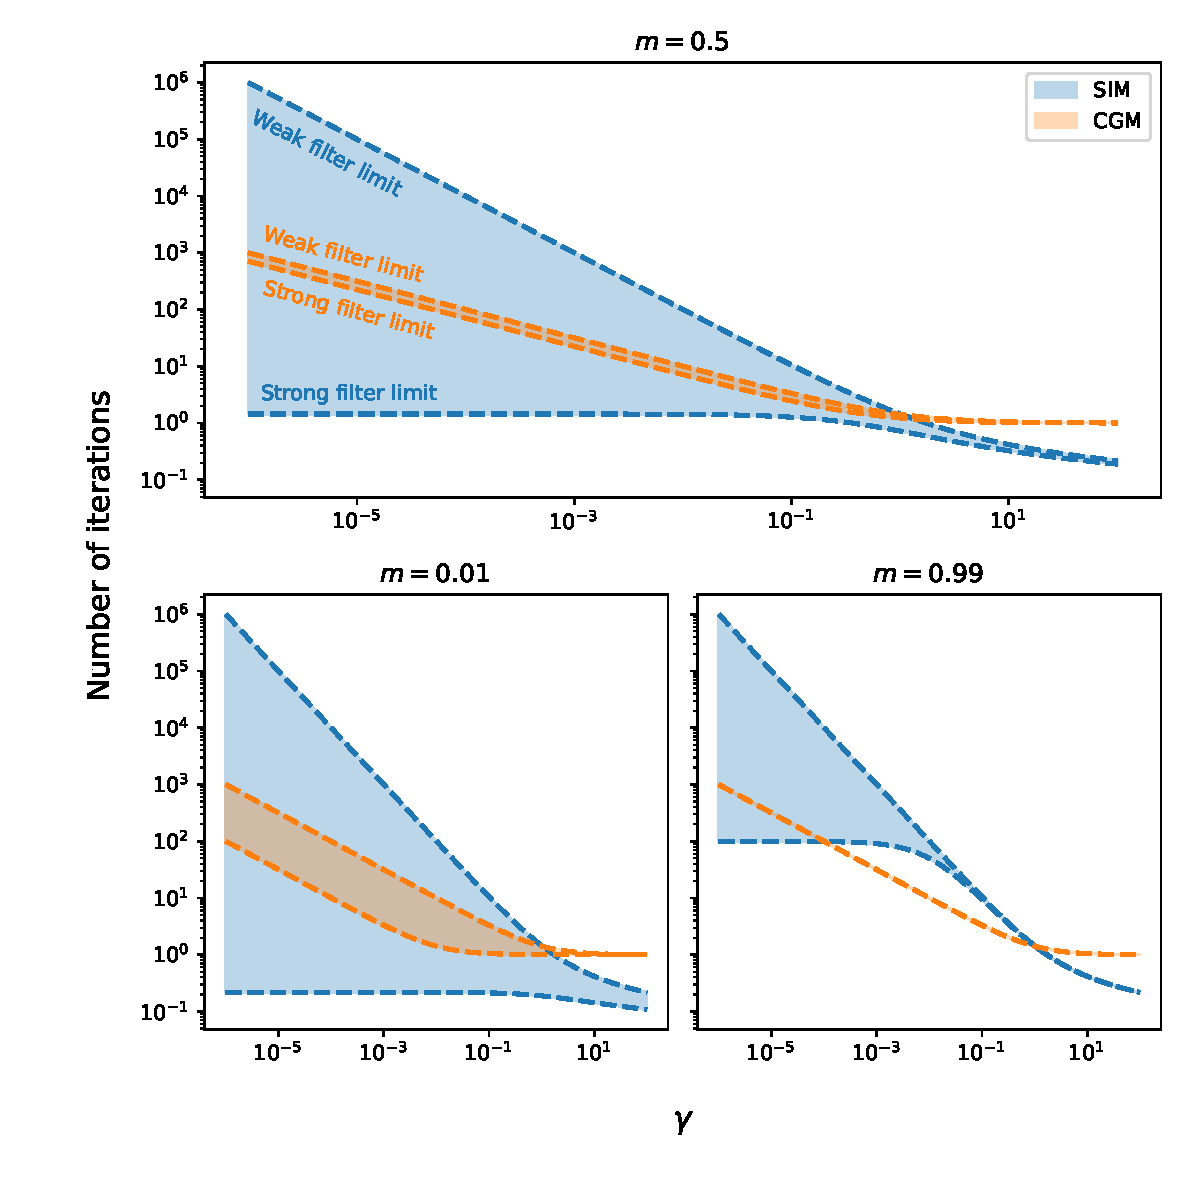
\includegraphics[width=0.85\linewidth]{Figures/conv_SIM_CGM_compared.pdf}
    \end{center}
    \caption{\small{ Here, we have plotted the functions given in \cref{eq:n_SIM_WFL,eq:n_CGM_WFL} } and \cref{eq:n_SIM_SFL,eq:n_CGM_SFL} to give a visual sense of the scaling rate of each method. Note that, since these functions are \textit{proportional} to the true number of iterations, the real values may be shifted up or down in this log-log plot.}
    \label{fig:conv_SIM_CGM_compared}
\end{figure}

In order to test the true convergence behaviour in practice, we ran a small experiment on synthetic data residing on a grid. In particular, we use a $16 \times 16$ grid of pixel data, and generated an observation matrix $\Y$ via white Gaussian noise. Next, for three different values of $m$, we chose pixels to be removed uniformly at random. We then counted the total number of iterations required to reconstruct the signal to a tolerance of $10^{-8}$ for both the SIM and the CGM, over a range of values of $\gamma$. This was done for four values of $\beta$, with a diffusion graph filter (see \cref{tab:iso_filters}). The results are shown in \cref{fig:it_gamma_plot}. 

\vspace{0.5cm}

\begin{figure}[hb]
    \begin{center} 
    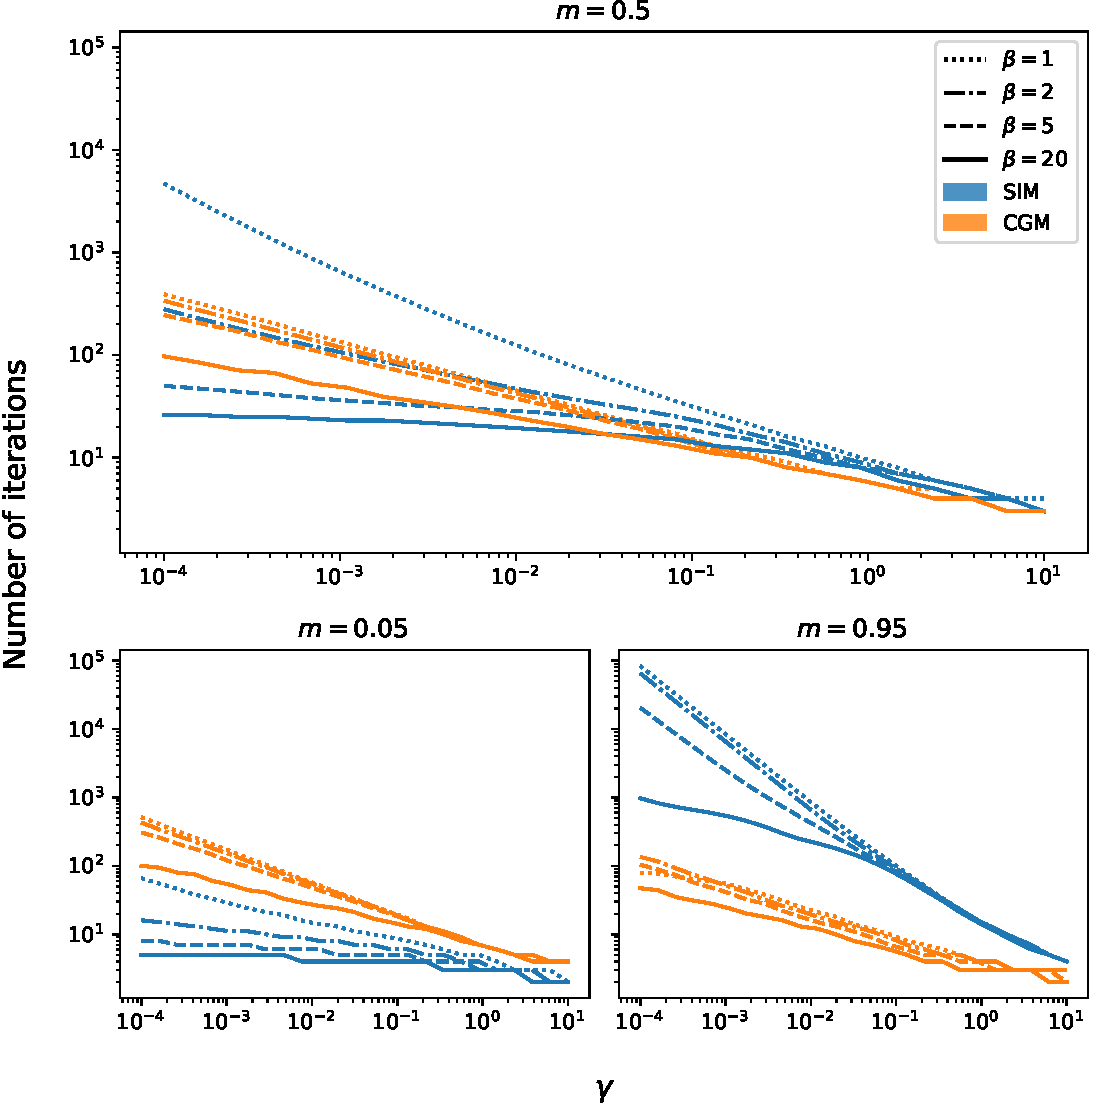
\includegraphics[width=0.9\linewidth]{Figures/experimental_its_for_conv.pdf}
    \end{center}
    \caption{\small{ The emprical number of steps required to reach some comparable convergence criteria is shown for a range of values of $\beta$ and $\gamma$ for both the SIM and CGM. Note that in all cases, $m=0.5$. }}
    \label{fig:it_gamma_plot}
\end{figure}

\vspace{0.5cm}

As is visible, the optimal choice of method will depend strongly on the choice of hyperparameters. Given these experiments, we give some ``rules-of-thumb'' for making this choice under various hyperparameter settings. This is summarised in \cref{tab:decision_SIM_CGM}. 


\begin{table*}[h]
    \centering
    \footnotesize
    \def\arraystretch{1.5}
    \begin{tabular}{@{}lccccccccccccc@{}}
    \toprule
    & \multicolumn{3}{c}{Small $\gamma$} & \phantom{ab} & \multicolumn{3}{c}{Medium $\gamma$} & \phantom{ab} & \multicolumn{3}{c}{Large $\gamma$} \\
    \cmidrule{2-4} \cmidrule{6-8} \cmidrule{10-12}
    & S $m$   & M $m$  & L $m$ &&  S $m$   & M $m$  & L $m$ && S $m$   & M $m$  & L $m$ && \\ \midrule \rule{0pt}{1cm}
    Small $\beta$  & SIM & CGM & CGM && SIM & CGM & CGM &&  SIM & CGM & CGM    \\ \rule{0pt}{6ex}
    Medium $\beta$ & SIM & SIM & CGM && SIM & CGM & CGM &&  SIM & CGM & CGM    \\ \rule{0pt}{6ex}
    Large $\beta$  & SIM & SIM & CGM && SIM & SIM & CGM &&  SIM & CGM & CGM   \\[0.5cm] \bottomrule 
    \end{tabular}
    \caption{This table gives a rough rule of thumb for which iterative method should be chosen under various hyperparameter settings. S, M and L $m$ refers to small, medium and large $m$. Note that small and large $m$ mean close to zero or one respectively, small and large $\gamma$ mean around $10^{-6}$ and around one respectively, and small and large $\beta$ mean values which cause the filter function to approach the weak and strong filter limits respectively. }
    \label{tab:decision_SIM_CGM} 
\end{table*}




 



% \begin{figure}[t]
%     % \begin{center} 
%     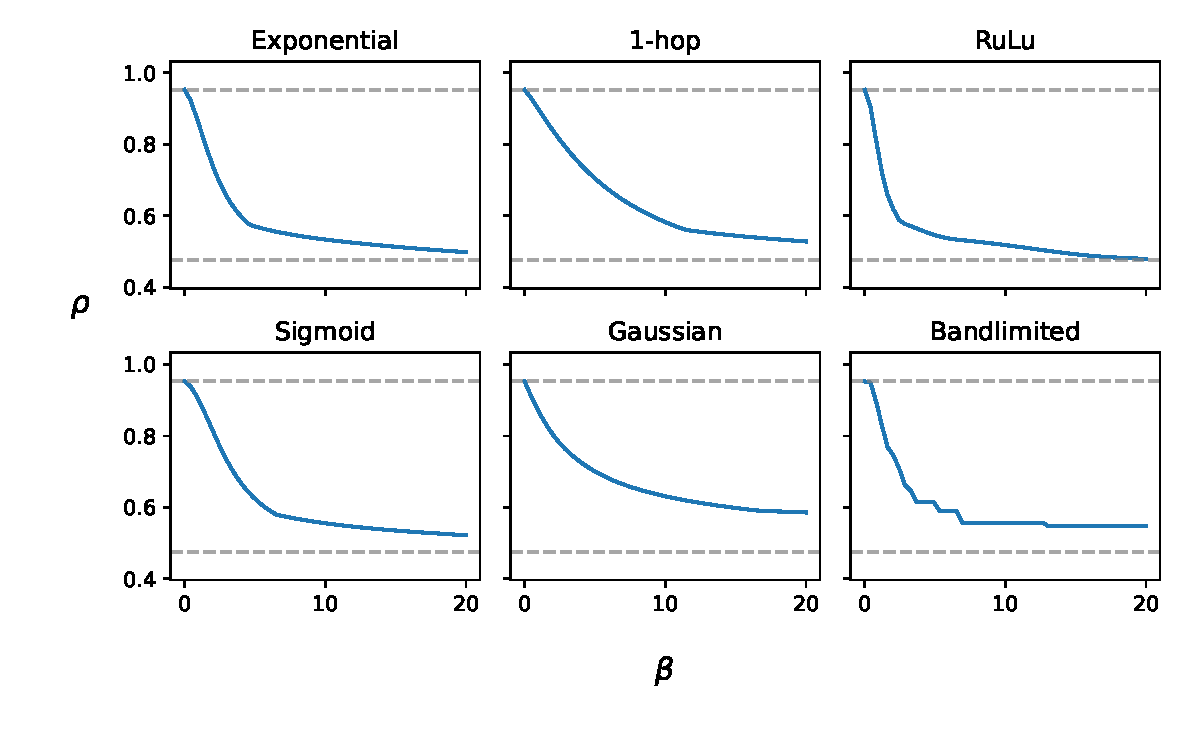
\includegraphics[width=0.88\linewidth]{Figures/beta-rho-plot.pdf}
%     % \end{center}
%     \caption{\small{ The emprical value of $\rho$ measured at different values of $\beta$ for six differnet filter types on a product graph defined by a $16 \times 16$ grid. Here,  $\beta$ is varied from 0 to 20 keeping $m$ fixed at 0.5. The upper and lower bounds given by the weak and strong filter limit respectively are indicated in gray. }}
%     \label{fig:beta_rho_plot}
% \end{figure}



\newpage


% \subsubsection{Characterising computational complexity}

% The number of steps required to reduce the magnitude of the error vector to some small value $\epsilon$ as a function of $\rho$ is given in \cref{eq:n_SIM}. Note that this applies in the case when the initial error vector $\vecc{\E_0}$ is proportional to the first eigenvector of $\M^{-1}\N$ and, as such, provides an upper bound.  


% Given the bounds on $\rho$ expressed in \cref{eq:rho_bounds}, it follows that the upper bound on the number of steps $n$ required for convergence is given by 

% \begin{equation}
%     \frac{-\log \epsilon}{\log(1 + \gamma) - \log m} \, \leq \, n \, \leq \, \frac{-\log \epsilon}{\log(1 + \gamma)}
% \end{equation}

% Note the taylor series expansions of these bounds around $\gamma=0$. 

% \begin{equation}
%     \label{eq:WFL_its}
%     \frac{-\log \epsilon}{\log(1 + \gamma)} = - \log \epsilon \left( \frac{1}{\gamma} + \frac{1}{2} - \frac{\gamma}{12} + O(\gamma^2) \right) 
% \end{equation}

% \begin{equation}
%     \label{eq:SFL_its}
%     \frac{-\log \epsilon}{\log(1 + \gamma) - \log m} = - \log \epsilon \left( -\frac{1}{\log m} - \frac{\gamma}{(\log m)^2} + O(\gamma^2)\right) 
% \end{equation}

% From this, it is clear that the convergence behaviour at small $\gamma$ is very different in these two cases. In particular, in the weak filter limit given in \cref{eq:WFL_its}, the number of iterations becomes dominated by the term $\gamma^{-1}$ which increases to infinity as $\gamma \rightarrow 0$. However, in the strong filter limit given in \cref{eq:SFL_its}, no such term exists meaning the number of iterations required for convergence is bounded as $\gamma \rightarrow 0$. This behaviour is depicted explicitly in \cref{fig:gamma_its}. Here, we plot the regularisation parameter $\gamma$ against the number of iterations required to reach some level of error. The dashed lines depict the predicted strong and weak filter limits, and the intermediate scattered points represent experimental values for iteration count over a range of values for $\beta$. 


% \begin{figure}[t]
%     % \begin{center} 
%     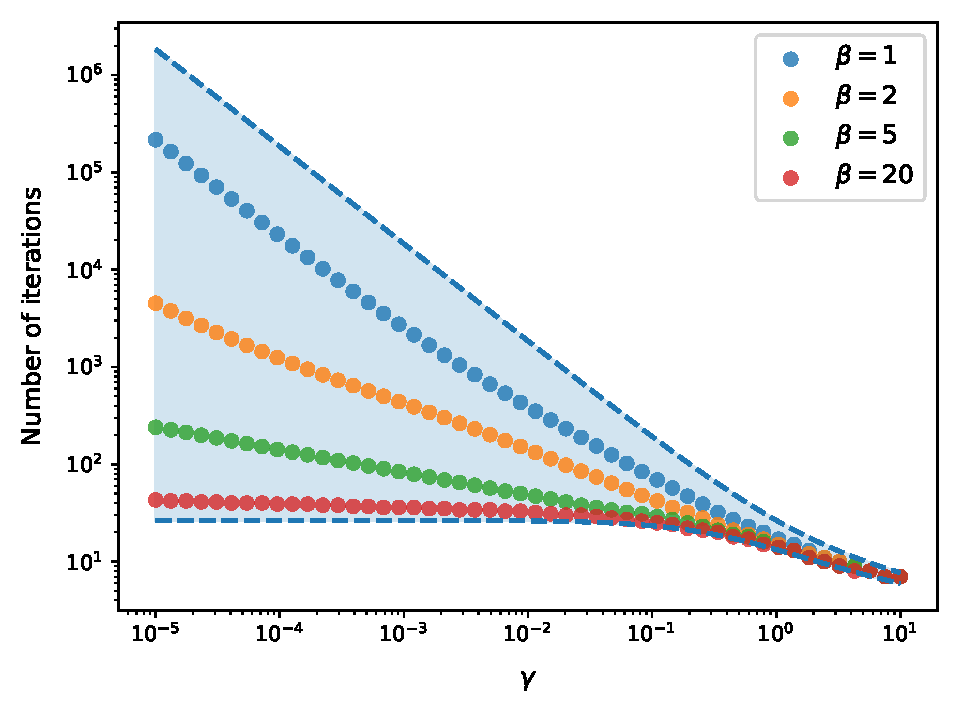
\includegraphics[width=0.8\linewidth]{Figures/it_gamma_plot.pdf}
%     % \end{center}
%     \caption{\small{ The number of iterations required to reduce the initial error magnitude by a factor of $10^{-8}$ is shown. The blue dashed lines represent the }}
%     \label{fig:gamma_its}
% \end{figure} 

% In conclusion, there is a hard upper bound for the computational complexity of the SIM: the limit of a weak filter. Since the SIM requires $O(N^2T + NT^2)$ multiplications per iteration, the complexity is given by


% \begin{equation}
%     \label{eq:OSIM}
%     O\Bigg(\frac{N^2T + NT^2}{\log\,(1 + \gamma)} \Bigg) \approx O\Bigg(\frac{N^2T + NT^2}{\gamma} \Bigg)
% \end{equation}


% In the limiting case of an infinitely strong filter, the computational complexity does not vary as a function of $\gamma$, but rather of the fraction of the data that is missing, $m$. 


% \begin{equation}
%     \label{eq:OSIM2}
%     O\Bigg(\frac{N^2T + NT^2}{\log\,(1 + \gamma) - \log m} \Bigg) \approx O\Bigg(\frac{N^2T + NT^2}{- \log m} \Bigg)
% \end{equation}

% For intermediately aggressive filters, the true computational complexity will be a function of all three of $\beta$, $\gamma$ and $m$. In general, fast convergence is associated with high values of $\beta$ and $\gamma$, and low values of $m$. 


% \subsection{Convergence of the CGM}
% \label{sec:CGM_convergence}

% In the conjugate gradient method, by contrast, the number of steps required to achieve some termination condition is well-known to follow $O(\sqrt{\kappa})$, where $\kappa$ is the condition number of the coefficient matrix \cite{Kelley1995}. In our case, the coefficient matrix is given in equation (\ref{eq:Z_post}) as $\C + \gamma \I$, and its associated condition number can be bounded in a similar fashion to $\rho$ in the SIM.

% Consider the definition for $\C$ given in equation (\ref{eq:Q}). Given this, we can write the condition number as 

% \begin{equation}
%      \kappa \left(  \, \D_\G \U \D_{\Ss} \U^\top \D_\G + \gamma \I \; \right)
% \end{equation}

% As in \cref{sec:SIM_convergence}, we will consider the limit of $\kappa$ as $\beta$ goes to both zero and infinity.  

% \subsubsection{Upper bound: the weak filter limit}

% Consider the limiting case of a weak filter where the parameter $\beta$ characterising the filter function approaches zero. In this case, the spectral scaling matrix $\G$ is full of ones and, as such, the diagonal matrix $\D_\G$ will be equal to the identity. Therefore 

% \begin{align}
%     \lim_{\beta \rightarrow 0} \quad \kappa \left(  \, \D_\G \U^\top \D_{\Ss} \U \D_\G + \gamma \I \; \right) &= \kappa  \left(  \, \U^\top \D_{\Ss} \U + \gamma \I \; \right) \notag \\[0.2cm]
%     &= \kappa  \left(  \, \U^\top \left( \D_{\Ss} + \gamma \I \right) \U \; \right) \notag \\[0.3cm]
%     &= \frac{1 + \gamma}{\gamma}
% \end{align}

% The number of steps required to achieve some level of precision will be proportional to $\sqrt{\kappa}$. The Taylor series expansion of this, as a function of $\gamma$ evaluated at zero gives

% \begin{equation}
%     \sqrt{\frac{1}{\gamma} + 1} = \gamma^{-1/2} \, + \, 
%     \frac{\gamma^{1/2}}{2} \, - \, \frac{\gamma^{3/2}}{8}  \, + \, O\left(\gamma^{5/2}\right) 
% \end{equation}


% This gives a hard limit on the computational complexity of the CGM as applied to graph signal reconstruction.



% \subsubsection{Lower bound: the srong filter limit}

% As with the SIM, consider now the limiting case where the parameter $\beta$ characterising the graph filter approaches infinity. In this case, the matrix $\G$ becomes $\mathbf{\Delta}$ as given in \cref{eq:Delta}. The condition number is therefore given by 

% \begin{align}
%     \lim_{\beta \rightarrow 0} & \quad \kappa \left(  \, \D_\G \U^\top \D_{\Ss} \U \D_\G + \gamma \I \; \right)  \notag \\[0.2cm]
%     &= \kappa  \left(  \, \D_{\mathbf{\Delta}} \U^\top \D_{\Ss} \U \D_{\mathbf{\Delta}}  + \gamma \I \; \right) \notag \\[0.3cm]
%     &= \kappa  \left(  \, 
%     \begin{bmatrix} 
%         \uu_1^\top \\ 
%         \mathbf{0}^\top \\
%         \vdots \\ 
%         \mathbf{0}^\top 
%     \end{bmatrix} \D_{\Ss}  \Big[ \uu_1, \, \mathbf{0}, \, \dots, \,\mathbf{0} \Big]
%     + \gamma \I \; \right) \notag \\[0.2cm]
%     &= \kappa  \left(  \, \frac{1}{NT}  \begin{bmatrix}
%         |\mathcal{S}'| & 0 & 0 & \dots \\
%         0 & 0 & 0 &  \\
%         \vdots & & & \ddots
%     \end{bmatrix}   + \gamma \I \; \right) \notag \\[0.3cm]
%     &= \frac{m + \gamma}{\gamma}
% \end{align}

% Again, evaluating the square root of the condition nu8}\left(\frac{m}{\gamma}\right)^{-3/2} \, + \, O\left(\left(\frac{m}{\gamma}\right)^{-5/2}\right) 
% \end{equation}

% In this case it is clear to see that the quantity of interest is $m/\gamma$. 


% \subsubsection{}

% $$
%     m \sqrt{\frac{1 + \gamma}{\gamma}} = m \Big( \frac{1}{\sqrt{\gamma}} + \frac{\gamma}{2\sqrt{\gamma}}  - \frac{\gamma^3}{8\sqrt{\gamma}} + ... \Big)
% $$

% From this expansion, we can see that the dominant behaviour for small $\gamma$ is $O(\gamma^{-1/2})$. Therefore, for small $\gamma$, the overall run-time complexity of the CGM is given by

% \begin{equation}
%     \label{eq:OCGM}
%     O\Bigg(\sqrt{\frac{1 + \gamma}{\gamma}}\big(N^2T + NT^2\big) \Bigg) \approx O\Bigg(\frac{N^2T + NT^2}{\sqrt{\gamma}} \Bigg)
% \end{equation}

% Furthermore, in the case of a time-vertex problem, or a
% mber in this  limit, gives the following Taylor series expansion. 

% \begin{equation}
%     \sqrt{\frac{m}{\gamma} + 1} = \left(\frac{m}{\gamma}\right)^{1/2} \, + \, \frac{1}{2}\left(\frac{m}{\gamma}\right)^{-1/2} \, - \, \frac{1}{8}\left(\frac{m}{\gamma}\right)^{-3/2} \, + \, O\left(\left(\frac{m}{\gamma}\right)^{-5/2}\right) 
% \end{equation}

% In this case it is clear to see that the quantity of interest is $m/\gamma$. 


% \subsubsection{}

% $$
%     m \sqrt{\frac{1 + \gamma}{\gamma}} = m \Big( \frac{1}{\sqrt{\gamma}} + \frac{\gamma}{2\sqrt{\gamma}}  - \frac{\gamma^3}{8\sqrt{\gamma}} + ... \Big)
% $$

% From this expansion, we can see that the dominant behaviour for small $\gamma$ is $O(\gamma^{-1/2})$. Therefore, for small $\gamma$, the overall run-time complexity of the CGM is given by

% \begin{equation}
%     \label{eq:OCGM}
%     O\Bigg(\sqrt{\frac{1 + \gamma}{\gamma}}\big(N^2T + NT^2\big) \Bigg) \approx O\Bigg(\frac{N^2T + NT^2}{\sqrt{\gamma}} \Bigg)
% \end{equation}

% Furthermore, in the case of a time-vertex problem, or a

\newpage 

\section{Conclusions}

In this chapter we have introduced a Bayesian model for the reconstruction of signals defined over the nodes of a Cartesian product graph. In particular, we show that the posterior mean of the smooth underlying signal, $\F$, is obtained by solving a linear system of size $NT \times NT$, given in \cref{eq:lin_system}. While a naive approach to computing this would have time complexity of $O(N^3T^3)$, we can utilise classic iterative methods in conjunction with the properties of the Kronecker product to solve the linear system with complexity $O(N^2T + NT^2)$ per iterative step. Furthermore, we show that this can be reduced to $O(N^2T + NT \log T)$ when considering time-vertex problems, and to $O(NT \log NT)$ when operating on a grid by making use of the Fast Cosine Transform (FCT). 

The key output of this chapter is two algorithms, namely the Stationary Iterative Method (SIM) and the Conjugate Gradient Method (CGM), tailored for the task of graph signal reconstruction. These were designed by making use of domain knowledge to produce a matrix splitting for the SIM and a preconditioner for the CGM that both guarantee bounded convergence. By analysing the spectral properties of the matrices involved in each algorithm, we provided a detailed overview of the expected convergence rate in both cases. The important results are summarised in \cref{tab:conv_SIM_CGM}, which gives a factor proportional to the number of iterations required for convergence in terms of the hyperparameters $\beta$, $\gamma$ and $m$. Given these results, we have provided some rules-of-thumb for making a choice of iterative method in practive, which is summaries in \cref{tab:decision_SIM_CGM}. This decision is of less importance when $\gamma$ is large, as both methods converge quickly in this domain, however it may be of great significance when $\gamma$ is small. 


\begin{table*}[h]
    \centering
    \def\arraystretch{1.5}
    \begin{tabular}{@{}cccccc}
    \toprule
    & \multicolumn{2}{c}{\textbf{SIM}} & \phantom{abc}& \multicolumn{2}{c}{\textbf{CGM}} \\
    \cmidrule{2-3} \cmidrule{5-6}
                               & All $\gamma$   & Small $\gamma$   &&  All $\gamma$   & Small $\gamma$ \\ \midrule \rule{0pt}{1cm}
    $\beta \rightarrow 0$      & $ \displaystyle \frac{1}{\log(1 + \gamma)}$   & $\displaystyle \gamma^{-1}$    &&    $\displaystyle \sqrt{\frac{1 + \gamma}{\gamma}}$ & $\displaystyle \gamma^{-1/2}$    \\ \rule{0pt}{6ex}
    $\beta \rightarrow \infty$ & $\displaystyle \frac{1}{\log(1 + \gamma) - \log m}$ & $\displaystyle -\frac{1}{\log m}$    &&  $\displaystyle \sqrt{\frac{1 - m + \gamma}{\gamma}}$ & $\displaystyle \left(\frac{\gamma}{1 - m} \right)^{-1/2}$ \\[0.5cm] \bottomrule 
    \end{tabular}
    \caption{The scaling behaviour of the number of steps required for convergence is shown as a function of $\gamma$ and $m$. The upper row gives the behaviour in the limit of a weak filter, and the lower row gives the behaviour in the limit of a strong filter. We also show the dominant term in the taylor expansion about $\gamma=0$ (``small $\gamma$" columns) which give a clearer picture of the asymptotic behaviour as $\gamma \rightarrow 0$. }
    \label{tab:conv_SIM_CGM} 
\end{table*}



    

% \section{Image processing experiments}

% \label{sec:im_proc_exp}


% \begin{figure}[t]
%     \hypertarget{runtime}{}
%     \label{fig:runtime}
%     \begin{center}
%         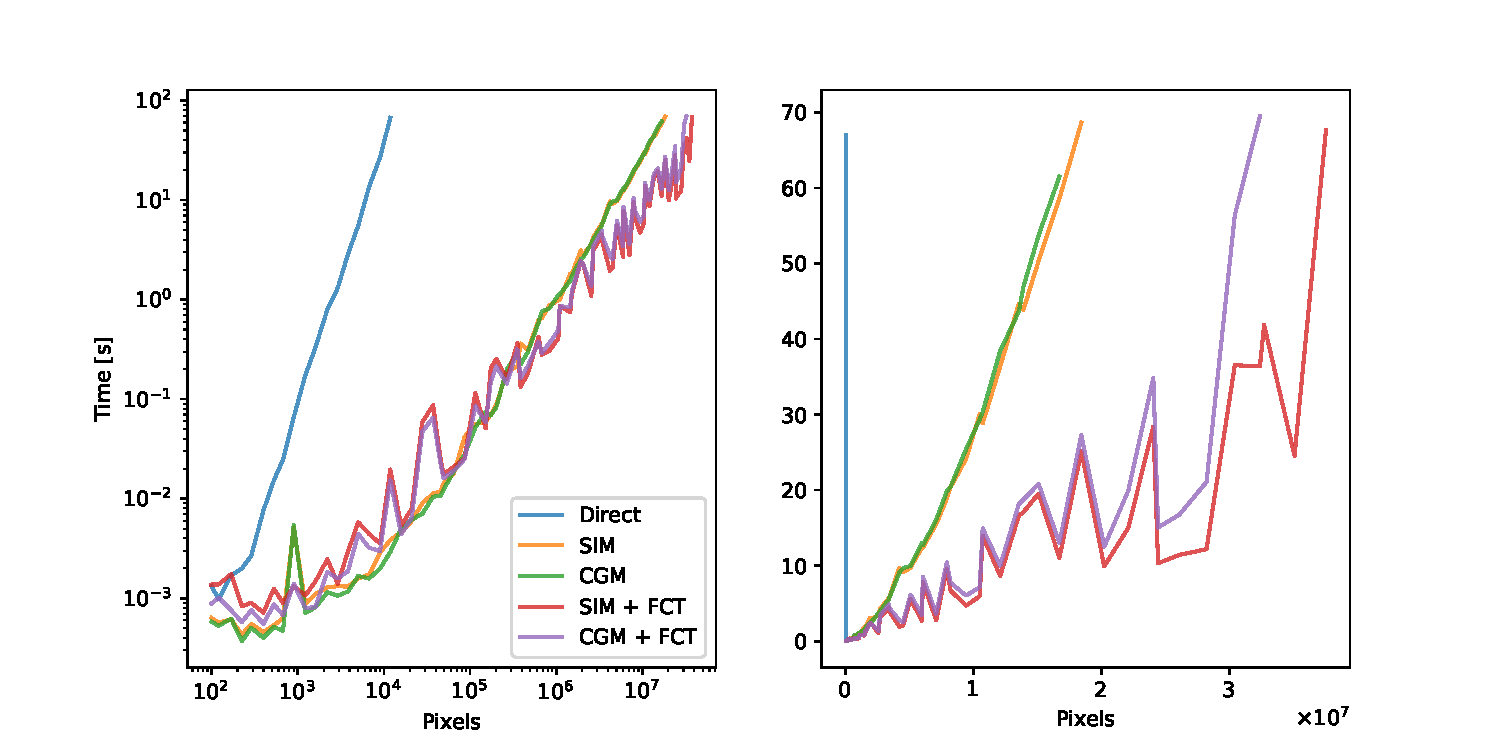
\includegraphics[width=\linewidth]{Figures/SIM_CGM_time.pdf}
%     \end{center}
%     \caption{\small{ The total runtime in seconds for the SIM and CGM compared to a naive Gaussian elimination approach is shown as a function of the total number of nodes using a quad-core Intel i7-7700HQ CPU. } }
% \end{figure}

% \begin{figure}[t]
%     \hypertarget{complexity}{}
%     \label{fig:complexity}
%     \begin{center}
%         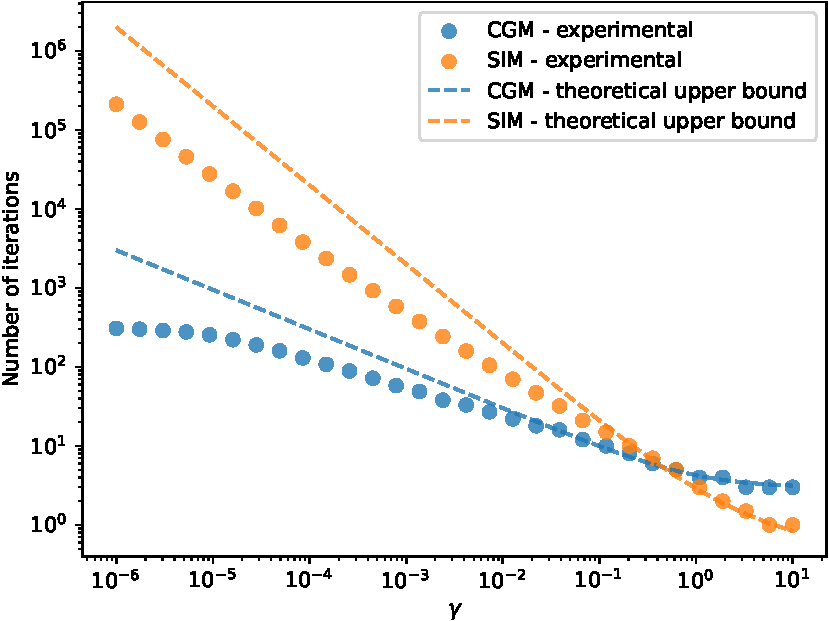
\includegraphics[width=0.7\linewidth]{Figures/complexity.pdf}
%     \end{center}
%     \caption{\small{The number of iterations required to reach a certain level of precision is shown experimentally, along with the theoretical upper bound, for the SIM and CGM} }
% \end{figure}



% % By comparing equations (\ref{eq:OSIM}) and (\ref{eq:OCGM}), we can see that the conjugate gradient method should be preferable at small $\gamma$.

% In this section, we run several small experiments to corroborate the properties of the CGM and SIM. In particular, we verify a) that both algorithms result in the same output for a given problem; b) that the runtime of the SIM and CGM increases at a significantly lower rate than naive Gaussian elimination as nodes are added; and c) that the number of iterations required for convergence as a function of $\gamma$ is less than or equal to the upper bounds derived in section \ref{sec:convergence}.

% In order to perform these checks, we use a small image denoising/reconstruction task. In particular, we use a grey-scale image of width 571 and height of 856 pixels which has been zero-centred and normalised. Note that an image can be considered a graph signal, with each pixel site representing a node connected to the other pixels immediately adjacent. Furthermore, the data itself lies on a two-dimensional lattice which is a special case of a product graph, with each sub-graph in the product being a simple chain, in this case with $N=856$ and $T=571$ respectively. Therefore, images can serve as a simple test case for checking the behaviour of product graph algorithms. Note that the purpose of this section is not to compare graph signal reconstruction to existing algorithms specialised for image denoising/reconstruction, but to examine the computational properties of GSR.

% First, we simulate a graph signal reconstruction task across a range of noise levels and missing data distributions. In particular, we add white Gaussian noise to the raw image with a Signal to Noise Ratio (SNR) of -10, 0 and 10 dB. We also remove pixels according to two rules. First, pixels are removed uniformly at random, and second, we remove entire rows and columns uniformly at random such that a fixed total percentage $p$ of the pixels is missing. We do this for $p$ equal to 0.01, 0.1, 0.25 and 0.5 giving 24 unique trials which are shown in \hyperlink{butterflies}{\textbf{figure 2}}. We find that both the SIM and the CGM converge quickly and result in identical predicted outputs, as expected. Furthermore, the statistical model seems relatively robust to noise and missing data of both types, visually performing adequately at the level of $p=0.5$ with SNR=-10dB, which is typically considered a challenging image reconstruction task.

% Next, we measured the total runtime of the SIM and the CGM as the number of nodes was increased, and compared this to a more naive approach to solving equation (\ref{eq:lin_system}) which is direct Gaussian elimination. In particular, we fixed the SNR at 0dB and the missingness to $p=0.5$, with missing pixels chosen uniformly at random, and created square images of increasing size from $10^2$ to $10^7$ total pixels. The results are shown in \hyperlink{runtime}{\textbf{figure 3}}. As is visible, the runtime of the SIM and CGM scales at a significantly slower rate that a naive approach, remaining tractable at well above $10^7$ nodes.

% Finally, we test the effect that varying the hyperparameter $\gamma$ has on the number of iterations required for convergence. To do this, we fixed the SNR at 0dB and the missingness to $p=0.5$, with missing pixels chosen uniformly at random. Next, we varied $\gamma$ in logarithmically spaced increments from $10^{-6}$ to $10^1$. For each unique value of $\gamma$, we ran both the SIM and the CGM and counted the number of steps required for each algorithm to reach a specific level of precision ($10^{-8}$ across all elements). The results are shown in \hyperlink{complexity}{\textbf{figure 4}}. We also plot the theoretical upper bound derived in the previous subsection for each method.

% As is visible, both methods converge within the bounds of their theoretical worst-case complexity. As expected, the CGM takes significantly fewer iterations than the SIM to converge at small $\gamma$. It is also visible that the CGM seems to outperform the theoretical worst-case scaling of $\gamma^{-0.5}$, converging with a rate closer to $\gamma^{-0.3}$ over the majority of the range, and even showing signs of reducing further at very small $\gamma$. The SIM on the other hand empirically converges slightly faster but close to the theoretical worst-case rate of $\gamma^{-1}$. Interestingly, the SIM converges faster than the CGM at relatively high $\gamma$, with the cross-over occurring at around $\gamma=0.5$. Although the absolute number of iterations required for convergence in this domain is low (between 1 and 10), this could still be significant for very large problems, meaning it still has some value as a solution.














\chapter{Regression and Reconstruction with Tensor-Valued
Multiway Graph Signals}

\lhead{Chapter 5. \emph{Regression and Reconstruction with
Multiway Graph Signals}}

\label{chap:nd_gsp}


Multiway Graph Signal Processing (MWGSP) is an emerging framework for analysing signals with multiple distinct axes (or `ways'), where the relation between elements within each axis is described by a graph topology \citep{Stanley2020}. For example, consider an fMRI experiment where cerebral blood flow is measured at a set of 3D voxels across time, for multiple subjects, in response to various stimuli. This dataset could be modelled as a six-way graph signal with the three spatial coordinates and the one time coordinate forming a four-way hypergrid graph, the subjects forming a graph based on characteristics, and the stimuli forming a graph based on similarity \citep{Cichocki2015}. A visual depiction of this is given in \cref{fig:fMRI_diagram}. 
 
\vspace{1.5cm}

\begin{figure}[h] 
    \begin{center}
        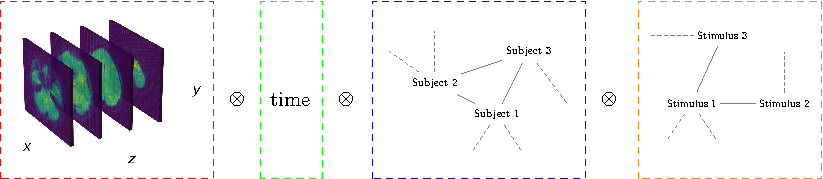
\includegraphics[width=\linewidth]{Figures/fMRI_Digaram.pdf}
    \end{center}
   \caption[Graphical depiction of an order-3 tensor]{Graphical depiction of a six-way graph signal originating from a hypothetical fMRI experiment. } 
    \label{fig:fMRI_diagram}
\end{figure} 


\begin{figure}[b] 
    \begin{center}
        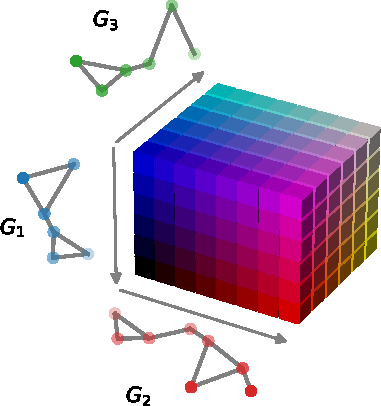
\includegraphics[width=0.4\linewidth]{Figures/coloured_tensor.pdf}
    \end{center}
   \caption[Graphical depiction of an order-3 tensor]{Graphical depiction of an order-3 tensor signal with graphs underlying each axis, which are linked together to form a Cartesian product graph.} 
    \label{fig:coloured_tensor}
\end{figure}  

The goal of this chapter is to extend the methods developed in \cref{chap:gsr_2d,chap:kgr_rnc_2d} such that they can accommodate multiway graph signals. In particular, Graph Signal Reconstruction (GSR), Kernel Graph Regression (KGR) and Regression with Network Cohesion (RNC) can all be understood as a special two-dimensional case of their more general MWGSP counterpart. In this chapter, we translate all three models into a their $d$-dimensional form, and demonstrate how to solve efficiently for the posterior mean.  


Multiway signals are described using tensors, which can be represented as $d$-dimensional arrays. Tensor algebra is well-established in fields such as physics and mechanics \citep{Renteln2013}, however it is less widespread in the graph signal processing community. As such, the first section of this chapter sets out some conceptual and notational standards regarding tensors, which are core to the present and proceeding chapters. 


We begin \cref{sec:dd_gsp} by defining the Cartesian product of more than two graphs, and discuss the algebraic and spectral structure of the resultant objects. Next, we cover the tensor representation of multiway graph signals and give the general definition of a graph-spectral operators in $d$-dimensions. We also discuss issues surrounding computational efficiency and how the so called `vec-trick', utilised in prior chapters, can be generalised to the tensor setting. In \cref{sec:tensor_gsr}, we begin the core contributions of this chapter by generalising Bayesian GSR as defined in \cref{chap:gsr_2d} to the MWGSP setting. This necessitates an updated version of the SIM and CGM to accommodate tensor-valued data in arbitrary dimensions, which we give in \cref{sec:SIM_dd,sec:CGM_dd}. Next, in \cref{sec:kgr_dd}, we generalise KGR for the non-parametric prediction of multiway graph signals as a function of exogenous variables. Finally, in \cref{sec:rnc_dd}, we the generalise RNC as defined in \cref{sec:rnc_mdp} in much the same way.  



\section{Multiway Graph Signal Processing}

\label{sec:dd_gsp}

\subsection{The Cartesian product of more than two graphs}

In \cref{sec:graph_products_defined} we gave the general definition of a product between two graphs and highlighted four standard examples, namely the Cartesian, direct, strong and lexicographic products. Each of these product types can be straightforwardly extended to more than two factor graphs by applying their respective definition recursively. For example, consider the Cartesian product between graphs $\mathcal{G}_A = \{\mathcal{V}_A, \mathcal{E}_A\}$, $\mathcal{G}_B = \{\mathcal{V}_B, \mathcal{E}_B\}$ and $\mathcal{G}_C = \{\mathcal{V}_C, \mathcal{E}_C\}$ where $|\mathcal{V}_A| = A$, $|\mathcal{V}_B| = B$ and $|\mathcal{V}_C| = C$. This can be written as 

\begin{equation}
    \mathcal{G} \; = \; \mathcal{G}_A \, \square \; \mathcal{G}_B \, \square \; \mathcal{G}_C \; = \; \{\mathcal{V}, \, \mathcal{E}\}
\end{equation}

The new vertex set, $\mathcal{V}$, is given by the Cartesian product of the individual vertex sets, arranged in lexicographic order. 

\begin{equation}
    \mathcal{V} = \mathcal{V}_A \times \mathcal{V}_B \times \mathcal{V}_C = \{(a, \, b, \, c) \in \mathbb{N}^3 \, | \, a \leq A, \; b \leq B, \text{and} \;  c \leq C\}
\end{equation}

The new edge set, $\mathcal{E}$, is given by recursively applying conditions 1 and 7 from, \cref{sec:graph_products_defined} to the new node set. In particular, any two nodes $(a, \, b, \, c)$ and $(a', b', c')$ are connected in $\mathcal{E}$ if they satisfy any of the following three conditions. 

\vspace{0.5cm}

\begin{table}[h]
    \def\arraystretch{1.5}
    \centering
    \begin{tabular}{lclclc}
        1. & $[a, \, a'] \in \mathcal{E}_A$    & and & $b = b'$  & and & $c = c'$             \\
        2. & $a = a'$    & and & $[b, \, b'] \in \mathcal{E}_B$   & and & $c = c'$             \\
        3. & $a = a'$    & and & $b = b'$  & and & $[c, \, c'] \in \mathcal{E}_C$              \\
    \end{tabular}
\end{table}


\begin{figure}[t]
    \begin{center}
        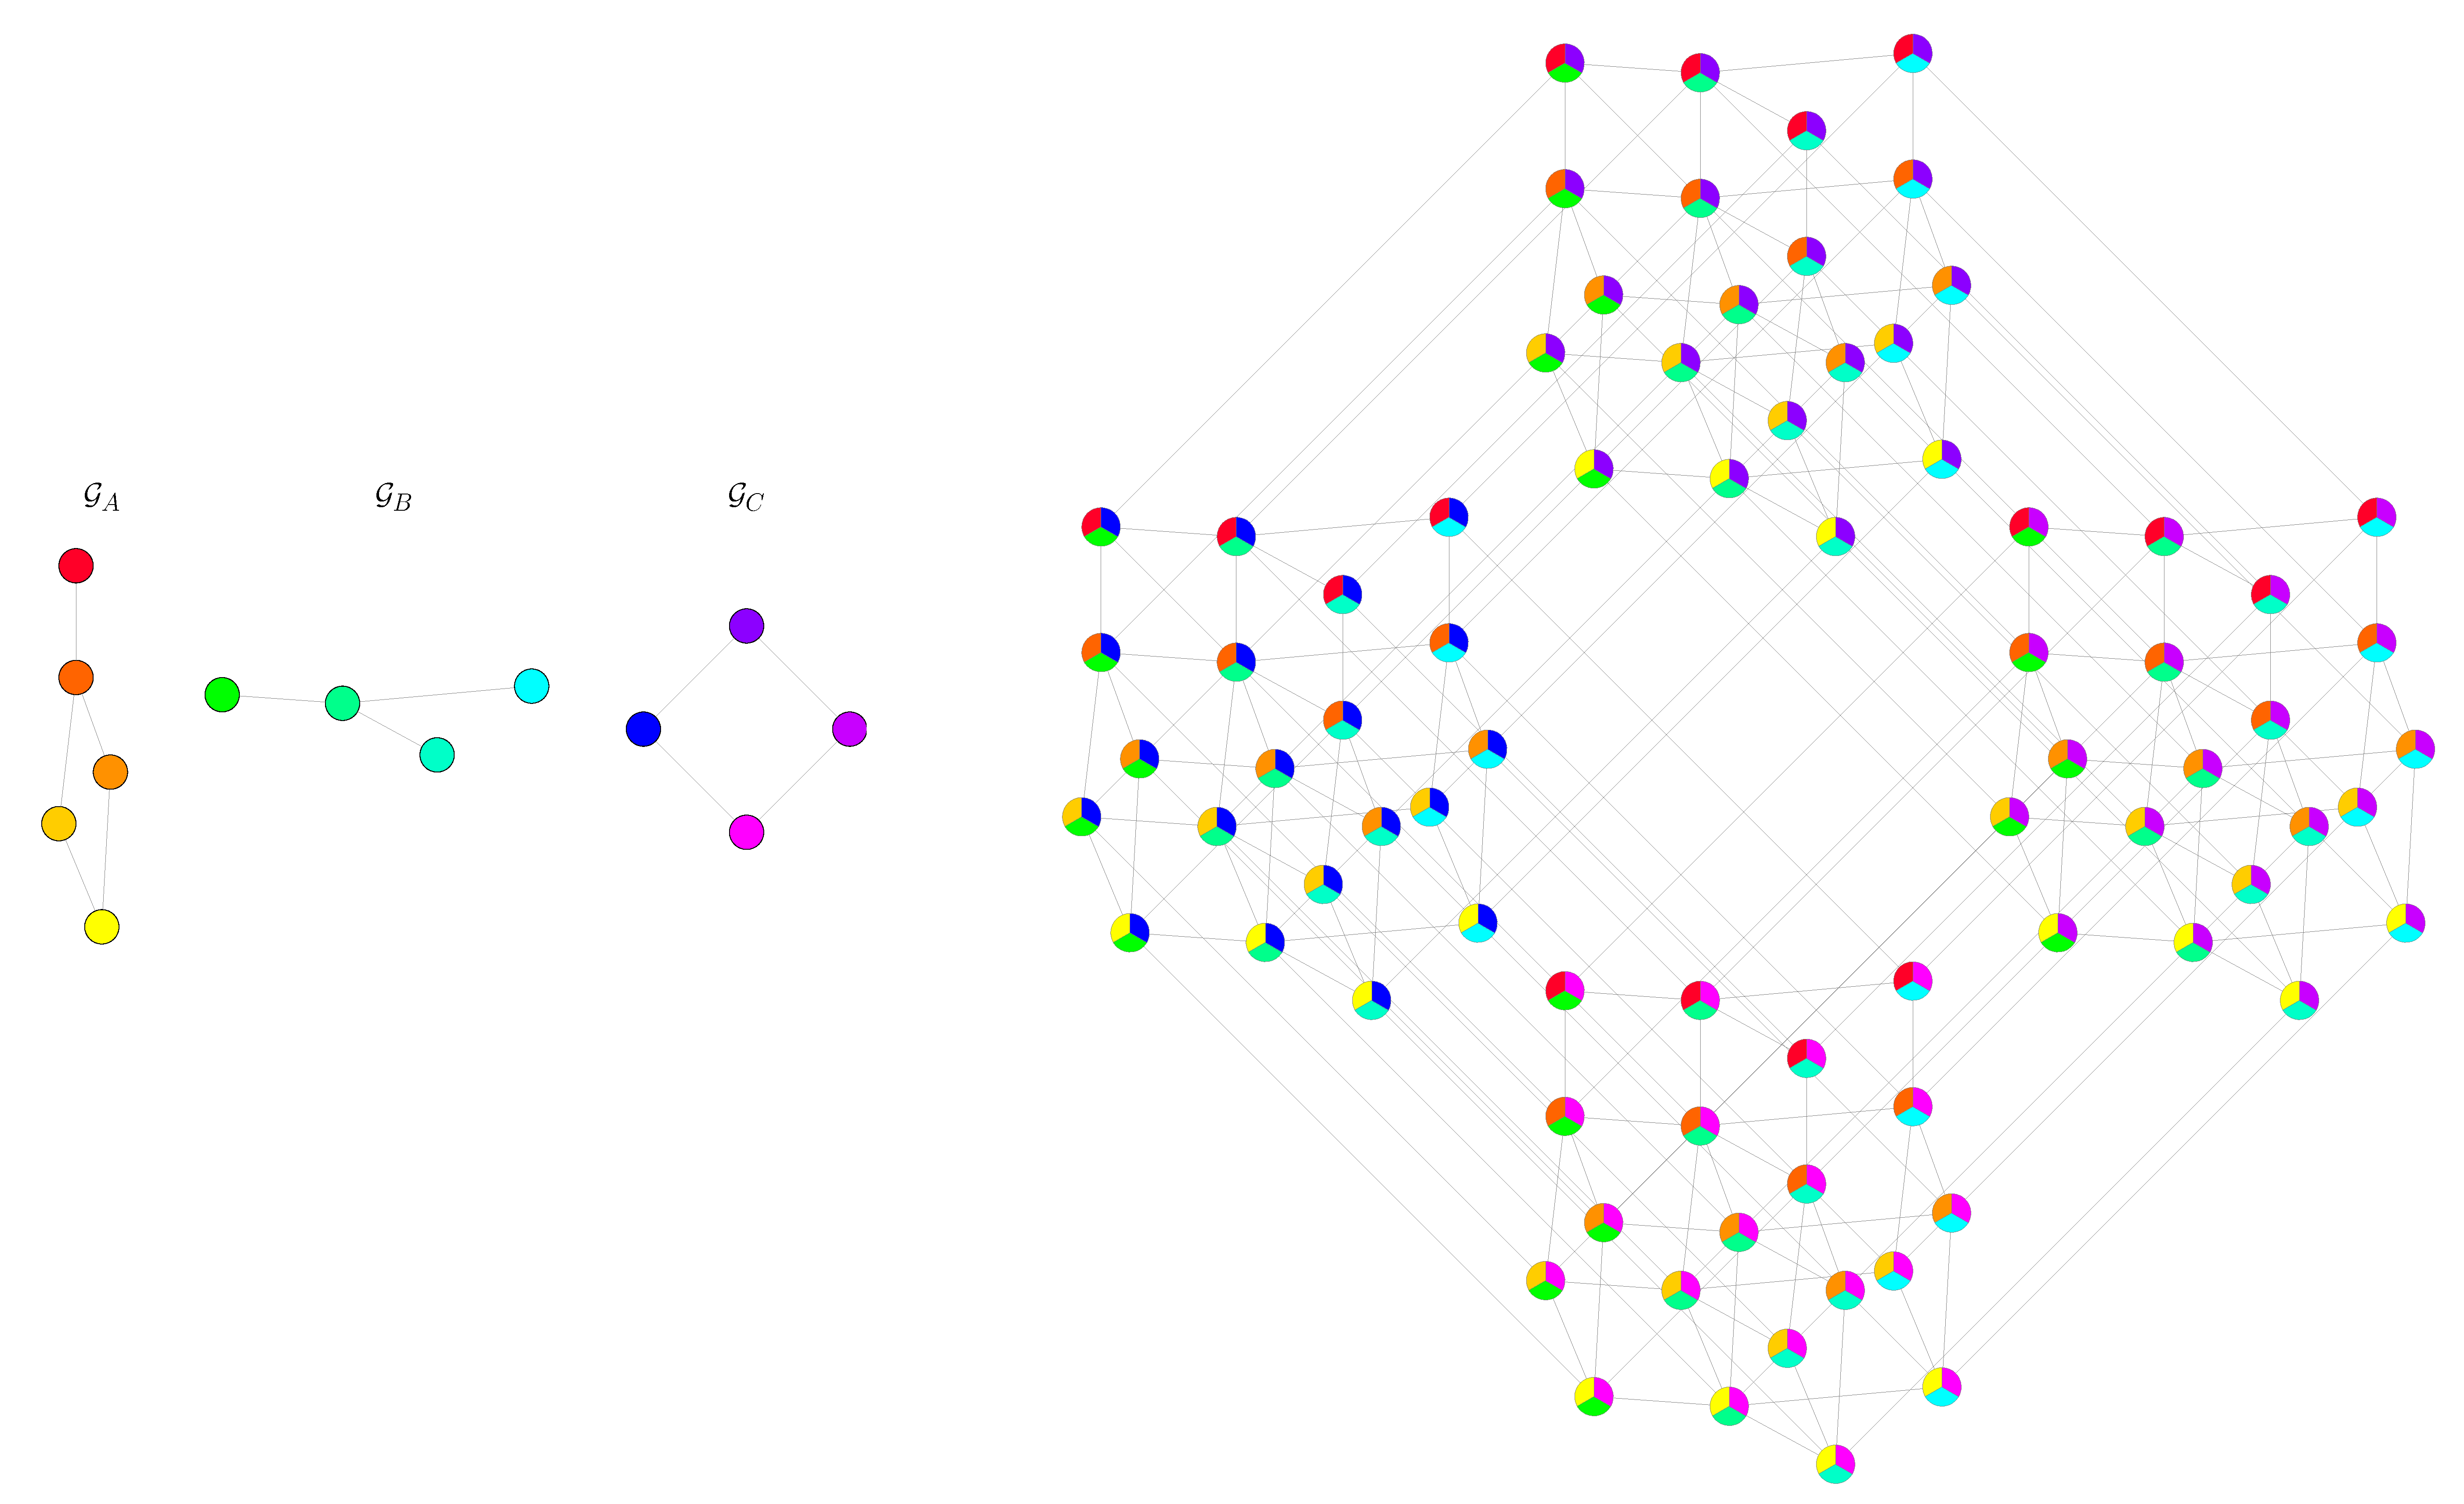
\includegraphics[width=\linewidth]{Figures/3D_CPG.pdf}
    \end{center}
    \caption[Graphical depiction of a 3D Cartesian product graph]{Graphical depiction of a 3D Cartesian product graph}
    \label{fig:3D_CPG}
\end{figure}

\Cref{fig:3D_CPG} gives a visual representation of a Cartesian product graph formed from three simple factor graphs. Notice that the size of the new vertex and edge set both grow very quickly. In particular, 

$$
|\mathcal{V}| = |\mathcal{V}_A| |\mathcal{V}_B| |\mathcal{V}_C| \aand |\mathcal{E}| =  |\mathcal{E}_A| |\mathcal{V}_B| |\mathcal{V}_C| + |\mathcal{V}_A| |\mathcal{E}_B| |\mathcal{V}_C| + |\mathcal{V}_A| |\mathcal{V}_B| |\mathcal{E}_C|
$$

Happily, the adjacency matrix of a Cartesian product graph $\A$ has a straightforward representation in terms of the factor adjacency matrices (here $\A_A$, $\A_B$ and $\A_C$). Specifically, it is given by their Kronecker sum. 

\begin{align}
    \A &= \A_A \oplus \A_B \oplus \A_C \notag \\
    &= \A_A \otimes \I_B \otimes \I_C  + \I_A \otimes \A_B \otimes \I_C + \I_A \otimes \I_B \otimes \A_C
\end{align}

In general, we can consider the Cartesian product of $d$ factor graphs with adjacency matrices denoted as $\A^{(1)} \in \R^{N_1 \times N_2}, \A^{(2)} \in \R^{N_2 \times N_2}, \dots \A^{(d)} \in \R^{N_d \times N_d}$. The full adjacency matrix will have size $N \times N$, where $N = \prod N_i$, and is given by  

\begin{alignat}{4}
    \A = \A^{(1)} & \oplus \A^{(2)} & \oplus \;\; ... \;\; & \oplus \A^{(d)} \notag \\[0.1cm]
    = \A^{(1)} & \otimes \I_{N_2} & \otimes \;\; ... \;\; & \otimes \I_{N_d} +  \notag \\[0.1cm]
    \I_{N_1} & \otimes \A^{(2)} & \otimes \;\; ... \;\; & \otimes \I_{N_d} + \;\; \ldots \;\; +  \notag \\[0.1cm]
    \I_{N_1} & \otimes \I_{N_2} & \otimes \;\; ... \;\; & \otimes \A^{(d)}  
\end{alignat}
    
This can be written compactly as 

\begin{equation}
    \A = \bigoplus_{i=1}^d  \A^{(i)}
\end{equation}

Similarly, the Laplacian of the product graph, $\LL$, can be written as the Kronecker sum of the individual factor graph Laplacians $\LL^{(i)}$. 

\begin{equation}
    \LL = \bigoplus_{i=1}^d  \LL^{(i)}
\end{equation}

We can perform eigendecomposition on each of the individual graph Laplacians as follows. 

\begin{equation}
    \LL^{(i)} = \U^{\,(i)} \LAM^{(i)} (\U^{\,(i)})^\top
\end{equation}

\noindent where $ \U^{(i)}$ is an orthogonal matrix such that each column is an eigenvector of $\LL^{(i)}$, and $\LAM^{(i)}$ is a diagonal matrix containing the corresponding eigenvalues, which are typically listed in ascending order. 

$$
\LAM^{(i)} = 
\begin{bmatrix}
    \lambda_1^{(i)}, &                 &        &                 \\
                     & \lambda_2^{(i)} &        &                 \\
                     &                 & \ddots &                 \\
                     &                 &        & \lambda_{N_i}^{(i)} \\
\end{bmatrix}
$$

Given this, the Laplacian of the product graph can be decomposed as follows. 

\begin{align}
    \LL &= \bigoplus_{i=1}^d \U^{\,(i)} \LAM^{(i)} (\U^{\,(i)})^\top \notag \\[0.2cm]
    &= \left( \bigotimes_{i=1}^d  \U^{\,(i)} \right) \left(\bigoplus_{i=1}^d \LAM^{(i)} \right) \left(\bigotimes_{i=1}^d  \U^{\,(i)} \right)^\top \notag \\[0.2cm]
    &= \U \LAM \U^\top 
\end{align}

\noindent where 

\begin{equation}
    \label{eq:U_LAM_def}
    \U =  \bigotimes_{i=1}^d  \U^{\,(i)} , \quad \text{and} \quad \LAM =  \bigoplus_{i=1}^d \LAM^{(i)}
\end{equation}


As with the Kronecker sum, here we have used the notation $\bigotimes_{i=1}^d  \U^{\,(i)}$ to denote the chained Kronecker product of matrices $\{\U^{\,(i)}  \}$. 

\subsection{Representing \textit{d}-dimensional graph signals}

Since each node in a $d$-dimensional product graph is specified by $d$ independent indices, a signal $\Yt$ existing over the nodes has a natural representation as a tensor of order $d$. One way to conceptualise a $d$-dimensional tensor signal is as a multi-dimensional array with $d$ independent axes. If the $i$-th factor graph has $N_i$ vertices, then $\Yt$ will be of shape $(N_1, \, N_2 , ... N_d)$. An individual element of this tensor signal can be specified via a vector index $\nn = [n_1,\, n_2,\, ...,\, n_d]$, where $1\leq n_i \leq N_i$.

Alternatively, signals can be represented as a vector of length $N = \prod N_i$. This is essential if we are to interpret the $\otimes$ symbol strictly as a Kronecker product, rather than a tensor or outer product. Under the Kronecker interpretation, the chained use of $\otimes$ used in expressions such as \cref{eq:U_LAM_def} results in matrices of shape $N \times N$, providing a linear map from $\R^{N} \rightarrow \R^{N}$. Therefore, for an operator to act on a tensor graph signal $\Yt \in \R^{N_1 \times N_2 \times ... \times N_d}$, we need a method of mapping tensors with shape $(N_1, \, N_2 , ... N_d)$ to vectors of length $N$. In order for this vectorisation process to be consistent with the operators, it should result in a vectors whose elements are arranged in lexicographic order. In some fields, this is referred to as \textit{row-major} vectorisation since, in the case of an order-2 tensor, the index representing the row varies before the column index. In the following, we symbolise this operation mathematically as $\vecrm{\cdot}: \R^{N_1 \times N_2 \times ... \times N_d} \rightarrow \R^N$, and its reverse operation as $\tenrm{\cdot}: \R^N \rightarrow \R^{N_1 \times N_2 \times ... \times N_d}$. We use the `RM' subscript to indicate explicitly that this process is occurring in row-major order, since the standard $\vecc{\cdot}$ function defined for matrices is most commonly assumed to act in column-major order.  

In the following, we use bold lower-case symbols (e.g. $\y$) to indicate graph signals existing in their vector form, and bold upper-case calligraphic symbols (e.g. $\Yt$) to indicate graph signals in their multi-dimensional array form. That is, 

\begin{align*}
    \y = \vecrm{\Yt} \quad \Longleftrightarrow \quad \Yt  = \tenrm{\y}
\end{align*}

\Cref{fig:ten_to_vec} shows gives a visual summary of the process of converting between these two representations for an order-3 tensor. 


\begin{figure}[t]
    \begin{center}
        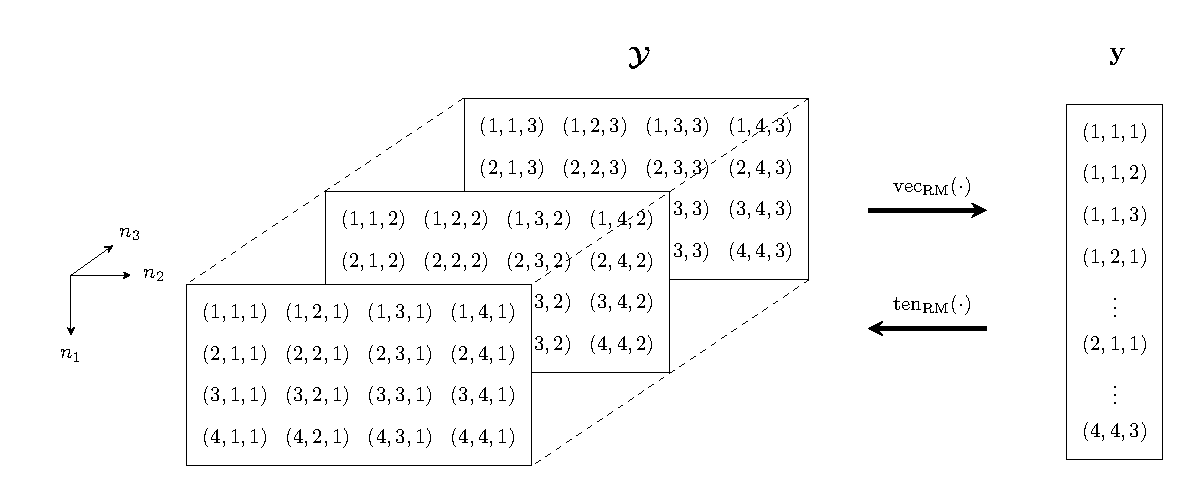
\includegraphics[width=\linewidth]{Figures/Tensor_Digaram.pdf}    
    \end{center}
    \caption[Conversion between a multidimensional array and a vector]{A graphical depiction of the process of converting an order-3 tensor between its multidimensional array and vector form in row-major order. Note that the elements in the vectorised signal are lexicographically ordered. }
    \label{fig:ten_to_vec}
\end{figure}


To calculate the vector index $k$ which a tensor element with index $\nn = [n_1,\, n_2,\, ...,\, n_d]$ is mapped to in row-major order, we can apply the following formula.  

\begin{equation}
    \label{eq:vec}
    k = 1 + \sum_{i=1}^d \Big( \prod_{j=i+1}^d N_j \Big) \, (n_i - 1)
\end{equation}

(Note the $\pm1$ disappear when indexing begins from zero). The reverse operation, i.e. mapping a vector element index $k$ to a tensor index $\nn$ can be achieved by running the algorithm \hyperlink{vectoten}{\textbf{3}}. 


\begin{algorithm}[b]
    \hypertarget{vectoten}{}
    \label{al:vectoten}
    \caption{Mapping a vector element to a tensor element in row major order}
    \begin{algorithmic}
    \vspace{0.15cm}
    \Require{The target vector element $k$} 
    \vspace{0.1cm}
    \Require{The shape of the output tensor $(N_1, N_2, ..., N_d)$} 
    \vspace{0.25cm}
    \State{$k \leftarrow  k - 1$}
    \vspace{0.25cm}
    \For{$i$ \textbf{from} $d$ \textbf{to} 1}
    \vspace{0.25cm}
    \State{$n_i \leftarrow  k \mod N_i$}
    \vspace{0.15cm}
    \State{$k \leftarrow \lfloor k / N_i \rfloor$} 
    \vspace{0.15cm}
    \EndFor
    \vspace{0.25cm}
    \Ensure{$(n_1 + 1, n_2 + 1, ..., n_d + 1)$}
    \end{algorithmic}
\end{algorithm}



Given these two operations, two arrays of any consistent shape can be mapped between one another by first vectorising according to \cref{eq:vec}, and then converting to a tensor using the given algorithm.



\subsection{GSP in \textit{d}-dimensions}

\label{sec:GSP_dd}

Consider a tensor graph signal $\Yt \in \R^{N_1 \times N_2 \times ... \times N_d}$ represented in its multi-dimensional array form. In direct analogy to the two dimensional case given in \cref{eq:GFT_2d,eq:IGFT_2d}, we can define the Graph Fourier Transform (GFT) and its corresponding inverse (IGFT) of this signal as follows. 

\begin{alignat}{2}
\label{eq:gft_nd}
    \text{GFT}(\Yt) & = \tenrm{\U^\top \y} && = \tenrm{\left(  \bigotimes_{i=1}^d  \U^{\,(i)} \right)^\top \vecrm{\Yt} } \\
\label{eq:igft_nd}
    \text{IGFT}(\Yt) & = \tenrm{\U \y} && = \tenrm{\left(  \bigotimes_{i=1}^d  \U^{\,(i)} \right) \vecrm{\Yt} }
\end{alignat}

The concept of a graph filter for signals defined on a Cartesian product graph follows naturally from this definition. Just as in the one and two-dimensional case, a graph filter is constructed by first taking the GFT of a signal, then applying some scaling function to each spectral component, then transforming back into the vertex domain via the IGFT. In the simplest case, we can consider an isotropic graph filter function $g(\lambda, \beta)$, such as one of those defined in \cref{tab:iso_filters}. A filter $\HH$, defined to act on a vectorised graph signal, can be represented as an $N \times N$ matrix, constructed as follows. 


\begin{align}
    \label{eq:H_def_dd}
    \HH &= \left( \bigotimes_{i=1}^d  \U^{\,(i)} \right) g\left(\bigoplus_{i=1}^d \LAM^{(i)}; \beta \right) \left(\bigotimes_{i=1}^d  \U^{\,(i)} \right)^\top \notag \\[0.2cm]
        &= \U \, \diag{\vecrm{\Gt}} \, \U^\top
\end{align}


Here, $\Gt$ represents the spectral scaling tensor, which has element $\nn = [n_1,\, n_2,\, ...,\, n_d]$ given by 

\begin{equation}
    \label{eq:Gn_dd1}
    \Gt_{\nn} = g\left(\sum_{i=1}^d \lambda^{(i)}_{n_i}; \, \beta\right)
\end{equation}

In certain special filter types, such as the diffusion filter, this function may be multiplicatively separable. In this case, we have that 

\begin{equation}
    \Gt_{\nn} = \prod_{i=1}^d g\left(\lambda^{(i)}_{n_i}; \, \beta\right)
\end{equation}

This further implies that the graph filter $\HH$ can be decomposed as 

\begin{equation}
    \HH = \bigotimes_{i=1}^d \HH^{(i)}, \where \HH^{(i)} = \U^{(i)} g \big(\LAM^{(i)}\big) \left(\U^{(i)}\right)^\top
\end{equation}

However, in the following, we typically don't consider this special case and assume that the graph filter function is non-separable in general. 

The concept of a multi-way graph filter can be further generalised to include anisotropic filter functions, where the intensity of the filtering operation is not restricted to be equal in each dimension. \Cref{tab:anis_filters} gives some examples of anisotropic graph filter functions defined to act in an arbitrary number of dimensions. 

\begin{table}[t]
    \def\arraystretch{1.7}
    \small
    \begin{center}
        \begin{tabular}{|l|c|}
            \hline
            \textbf{Filter}   & $g(\lambdaa; \,\betaa)$                                            \\
            \hline
            1-hop random walk & $(1 + \betaa^\top\lambdaa)^{-1}$                                   \\
            \hline
            Diffusion         & $\exp(-\betaa^\top\lambdaa)$                                       \\
            \hline
            ReLu              & $\max (1 - \betaa^\top\lambdaa, 0)$                                \\
            \hline
            Sigmoid           & $2 \big( 1 + \exp(\betaa^\top\lambdaa)\big)^{-1}$                  \\
            \hline
            Bandlimited       & $1, \,\text{if} \; \betaa^\top\lambdaa \leq 1 \; \text{else} \; 0$ \\
            \hline
        \end{tabular}
    \end{center}
    \caption{Anisotropic graph filter functions in an arbitrary number of dimensions}
    \label{tab:anis_filters}
\end{table}


In this case, the spectral scaling tensor is given by 

\begin{equation}
    \label{eq:Gn_dd2}
    \Gt_{\nn} = g\big(\lambdaa(\nn); \, \betaa\big)
\end{equation}

where $\betaa \in \R^{d}$ is the parameter vector characterising the filter intensity in each dimension, and $\lambdaa(\nn) \in \R^d$ is a vector holding the $n_i$-th eigenvalue of each graph Laplacian in the Cartesian product. 

\begin{equation}
    \label{eq:lam_of_n}
\lambdaa(\nn) = 
\begin{bmatrix}
    \lambda^{(1)}_{n_1} & \lambda^{(2)}_{n_2} & \dots & \lambda^{(d)}_{n_d}    
\end{bmatrix}^\top
\end{equation}

In general, we can define any spectral transformation in tensor terms as follows. 

\begin{equation}
    \Yt' = \text{IGFT} \left( \Gt \circ \text{GFT}(\Yt) \right)
\end{equation}

\subsection{Fast computation of the \textit{d}-dimensional GFT and IGFT}

\label{sec:fast_kron_dd}

Consider the definition of the GFT and IGFT of a $d$-dimensional graph signal given in \cref{eq:gft_nd,eq:igft_nd}. In both cases, we are required to compute the result of a chained Kronecker product matrix acting on a length-$N$ vector. Whilst the obvious approach to computing this product would have time and memory complexity of $O(N^2)$, a much more efficient implementation can be achieved by taking advantage of the Kronecker structure of the matrix. Specifically, the memory and time complexity of this operation can be reduced to $O(N)$ and $O(N\sum N_i)$ respectively. The importance of this fact cannot be understated, as it enables scaling to much larger product graphs that would otherwise be possible. 

This general algorithm for achieving this is well-known, and can be summarised as follows. Consider the application of a chained Kronecker product matrix acting on a vector $\y$. 

$$
\y = \left( \U^{(1)} \otimes \U^{(2)} \otimes ... \otimes \U^{(d)}\right) \z
$$

This can be factorised as follows

$$
\y = \left( \U^{(1)} \otimes \I \otimes ... \otimes \I \right)\left( \I \otimes \U^{(2)} \otimes ... \otimes \I \right) ... \left( \I \otimes \I \otimes ... \otimes \U^{(d)} \right) \z
$$

As is visible, the original multiplication has now been broken into $d$ stages. However, the $i$-th stage can be completed with $N \times N_i$ multiplications by reshaping the vector in the appropriate way and leveraging the properties of the Kronecker product. The reshaping operation can be completed using strided permutation matrices which can be applied in practice for virtually zero computational cost \citep{Granata1992}. This idea is also key to the FFT and related algorithms, which can be understood as finding a recursive Kronecker structure in the Fourier matrix \citep{Tolimieri2013}. 

Work on efficient computational procedures for this operation can be traced back to \cite{Roth1934} who formulated the original 2-dimensional ``vec trick" algorithm. The $d$-dimensional generalisation was proposed in \cite{Pereyra1973} and improved in \cite{DeBoor1979}. More recent work, such as \cite{Fackler2019}, has focused on further optimisations such as minimising data transit times and parallel processing. 

Furthermore, if the $i$-th factor graph in the Cartesian product is a path or ring graph, then the corresponding matrix transformation can be completed with only $N \log N_i$ multiplications by making use of the FCT/FST/FFT algorithms. In the extreme case, where every factor graph has this special structure, the computational complexity reaches parity with the multidimensional FFT algorithm, and will have a runtime complexity of $O(N \log N)$ \citep{Smith1995}. 

In order to execute computations of this nature in a way that is maximally efficient, we have developed the Python library \textit{PyKronecker}, which is described in detail in \cite{Antonian2023}. This library offers a high-level API for constructing Kronecker-based operators and applying them to either vectors or tensors, whilst optimising the underlying computation using parallel GPU processing and Just In Time (JIT) compilation using the Jax library \citep{Bradbury2018}. In the following, it will be assumed that all chained Kronecker product matrices are applied to vectors/tensors using an efficient implementation. This is essential for computing the $d$-dimensional GFT and IGFT, the basic pseudocode for which is shown in algorithm \hyperlink{al:GFT_dd}{\textbf{4}}. Note that the `reshape' operation should always be applied using the row-major convention. This is the standard convention in languages such as C and Python's NumPy library \citep{Harris2020}, but not in languages such as Matlab and Fortran. 

\begin{algorithm}[t]
    \hypertarget{al:GFT_dd}{}
    \label{al:GFT_dd}
    \caption{Efficient GFT and IGFT in $d$-dimensions}
    \begin{algorithmic}
    \vspace{0.25cm}
    \Require{List of Laplacian eigenvector matrices $\left\{\U^{(i)} \in \R^{N_{i} \times N_{i}}\right\}_{i=1}^d$} 
    \vspace{0.8cm}
    \Function{GFT}{$ \Yt \in \R^{N_1 \times N_2 \times ... \times N_d} $}
    \vspace{0.25cm}
    \For{$i$ \textbf{from} 1 \textbf{to} $d$}
    \vspace{0.25cm}
    \State{$\Yt\leftarrow \text{reshape}\Big(\Yt,  \;\big(N_i,\, N / N_i \big) \Big)$}
    \vspace{0.25cm}
    \State{$\Yt \leftarrow \left( \left(\U^{(i)}\right)^\top \; \Yt  \right)^\top$} 
    \vspace{0.25cm}
    \EndFor
    \vspace{0.25cm}
    \State{\textbf{return} $\text{reshape}\Big(\Yt, \; \big(N_1, \, N_2, \; ..., \; N_d \big) \Big)$}
    \vspace{0.25cm}
    \EndFunction
    \vspace{1cm}
    \Function{IGFT}{$ \Zt \in \R^{N_1 \times N_2 \times ... \times N_d} $}
    \vspace{0.25cm}
    \For{$i$ \textbf{from} 1 \textbf{to} $d$}
    \vspace{0.25cm}
    \State{$\Zt\leftarrow \text{reshape}\Big(\Zt,  \;\big(N_i,\, N / N_i \big) \Big)$}
    \vspace{0.25cm}
    \State{$\Zt \leftarrow \left( \U^{(i)} \; \Zt  \right)^\top$} 
    \vspace{0.25cm}
    \EndFor
    \vspace{0.25cm}
    \State{\textbf{return} $\text{reshape}\Big(\Zt, \; \big(N_1, \, N_2, \; ..., \; N_d \big) \Big)$}
    \vspace{0.25cm}
    \EndFunction
    \vspace{0.25cm}
    \end{algorithmic}
\end{algorithm}


\note{A note on tensor notation}{
    The use of tensor algebra is well established in fields such as phyics and mechanics \citep{Renteln2013,Abraham1988}, however, it is less widespread in the signal processing community. For this reason, we choose to adopt a notation that leans more on standard linear algebra, however, all the equations and algorithms discussed in the following chapters could be alternatively written in a purer form of tensor notation. For example, consider the IGFT of a tensor signal $\Zt$. In our notation, this is written as

    \vspace{0.3cm}

    \begin{equation}
        \label{eq:LA_MM}
        \Yt = \text{ten}_{\text{RM}}\left(\left(\bigotimes_{i=1}^d  \U^{\,(i)}\right) \text{vec}_\text{RM}\left(\Zt\right) \right)    
    \end{equation}

    \vspace{0.3cm}

    As is visible, this describes the process in terms of regular matrix-vector multiplication, but requires the additional definition of the $\vecrm{\cdot}$ and $\tenrm{\cdot}$ operations. Alternatively, this expression could be written using tensor indexing and Einstein summation notation as follows. 
    
    \vspace{0.3cm}

    \begin{equation}
    \label{eq:TEN_MM}
    \Yt^{\, i_1, i_2, ..., i_d} = \left(\U^{(1)}\right)^{i_1}_{j_1}\left(\U^{(2)}\right)^{i_2}_{j_2} ... \left(\U^{(d)}\right)^{i_d}_{j_d} \, \Zt^{\, j_1, j_2, ..., j_d}
    \end{equation}

    \vspace{0.3cm}

    Note that here the indices $j_1, j_2, ..., j_d$ on the right hand side are implicitly summed over. This eliminates the need to consider vectorisation at all and is perhaps a more elegant way of describing the $d$-dimensional GFT/IGFT. However, there are multiple indices to keep track of which becomes somewhat unaesthetic in a variable number of dimensions.

    \vspace{0.3cm}
    
    Both forms offer different trade-offs, however, there is no practical difference when it comes to executing the signal precessing algorithms themselves. Note that, as described in \cref{sec:fast_kron_dd}, the full $N \times N$ matrix implied by \cref{eq:LA_MM} is never actually instantiated in memory (see algorithm \hyperlink{KronMatMul}{\textbf{4}}).

}

\section{Multiway Graph Signal reconstruction}

\label{sec:tensor_gsr}

The model we use to describe graph signal reconstruction in the multi-dimensional setting is as follows. Consider a tensor signal $\Yt$ of shape $\big(N_1, \, N_2, \, ... \, N_d \big)$ with elements interpreted as existing on the nodes of a $d$-dimensional Cartesian product graph. Only a partial set $\mathcal{S} = \{\nn_1, \, \nn_2, \, ... \}$ of the vector elements of $\Yt$ are available at observation time, with unobserved values set to zero. The goal is to estimate the signal value at these unobserved entries. 

To aid with the model description, we also introduce a binary sensing tensor $\St$, of the same shape as $\Yt$, which is used to indicate which elements of $\Yt$ were observed. This is defined as follows.  

\begin{equation}
    \St_{\nn} = \begin{cases}
        1 & \text{if} \;\; \nn \in \mathcal{S} \\
        0 & \text{otherwise}
    \end{cases}
\end{equation}

The input data for signal reconstruction on a $d$-dimensional Cartesian product graph can therefore be summarised as follows. 

\begin{equation*}
    \text{input data} = \Big\{\; \Yt \in \R^{N_1 \times ... \times N_d}, \;\; \St \in \{0, 1\}^{N_1 \times ... \times N_d} , \;\; \LL \in \R^{N \times N} \; \Big\}
\end{equation*}

In analogy with the two dimensional case, (see \cref{sec:problem_statement_2d}), we assume that $\Yt$ is a noisy partial observation of an underlying tensor, $\Ft$, which is smooth with respect to the topology of the Cartesian product graph. This is represented by the following statistical model. 

\begin{equation}
    \Yt = \St \circ \big(\Ft + \Et \big)
\end{equation}

where, here, the $\circ$ symbol represents the generalised tensor Hadamard product, i.e. element-wise multiplication of two tensors. $\Et$ is a random tensor where each element has an independent normal distribution with with unit variance. That is,

\begin{equation}
    \vecrm{\Et} \, \sim \, \Norm{\zero}{\I_N}
\end{equation}

Given this distribution over the model noise, the conditional distribution of $\Yt |  \Ft$ is given by 

\begin{equation}
    \vecrm{\Yt} \, | \, \vecrm{\Ft} \, \sim \, \mathcal{N}\Big(\vecrm{\St \circ \Ft}, \; \diag{\vecrm{\St}}\Big)
\end{equation}

Or, more concisely, 

\begin{equation}
    \y \, | \, \f \, \sim \, \mathcal{N}\big(\s \circ \f, \; \D_{\St} \big)
\end{equation}

where $\f = \vecrm{\Ft}$, $\y = \vecrm{\Yt}$ , $\s = \vecrm{\St}$ and $\D_{\St} = \diag{\s}$. In order to encode the belief that the underlying tensor $\Ft$ is smooth with respect to the topology of the graph, we can make use of the following prior distribution. 

\begin{equation}
    \f \, \sim \, \mathcal{N}\left( \zero, \, \gamma^{-1} \HH^2 \right) 
\end{equation}

where $\HH$ is constructed from a graph filter function in the manner specified in \cref{eq:H_def_dd}, i.e.

\begin{equation*}
    \HH = \U \D_\Gt \U^\top
\end{equation*}

where $\D_\Gt = \diag{\vecrm{\Gt}}$, and $\Gt$ is the spectral scaling matrix obtained by applying a graph filter to the graph Laplacian eigenvalues. The intuition for this prior can be obtained from a direct generalisation of the one and two dimensional cases. In essence, tensor signals drawn from this prior will have the same probability density function as iid noise filtered by $\HH$, so samples will be naturally smooth with respect to the topology of the underlying Cartesian product graph. By applying Bayes theorem, we obtain the posterior distribution for $\f$ conditioned on $\y$. 


\begin{equation}
    \f \, | \, \y \sim \Norm{\PP^{-1} \y}{\PP^{-1}}
\end{equation}

where 

\begin{equation}
    \PP = \D_{\St} + \gamma \HH^{-2}
\end{equation}

Therefore, the mean of this posterior is obtained by solving the following linear system.

\begin{equation}
    \label{eq:lin_system_dd}
    \f^{\star} = \left(\D_\St + \gamma \HH^{-2}\right)^{-1} \y
\end{equation}

Once again, we are faced with a similar set of problems to those outlined in \cref{sec:problem_statement_2d}. Namely, the coefficient matrix is very large and potentially ill-defined. This can be solved by turing to iterative methods such as the SIM and CGM, which are repeated here in their form adapted for the general tensor case. 

\subsection{Tensor SIM}

\label{sec:SIM_dd}

Generalising the SIM, which we describe in \cref{sec:SIM}, to the tensor setting is straightforward. In particular, \cref{eq:lin_system_dd} can be solved by splitting the coefficient matrix $\left(\D_\St + \gamma \HH^{-2}\right)$ into $\M - \N$, where $\M$ and $\N$ take on the following values
 
\begin{equation}
    \M = \gamma \HH^{-2} + \I_N, \aand \N = \D_{\St'}
\end{equation}

where $\D_{\St'} = \diag{\mathbf{1} - \s}$. In this case, the inverse of $\M$ has the form 


\begin{align}
\M^{-1} &= \left( \bigotimes_{i=1}^d  \U^{\,(i)} \right) \, \diag{\vecrm{\Jt}}\, \left(\bigotimes_{i=1}^d  \U^{\,(i)} \right)^\top \notag \\[0.2cm]
&= \U \, \D_\Jt \, \U^\top
\end{align}

where the tensor $\Jt$ has entries with the vector index $\nn = [n_1,\, n_2,\, ...,\, n_d]$ given by 

\begin{equation}
    \Jt_{\nn} = \frac{\Gt_{\nn}^2}{\Gt_{\nn}^2 + \gamma}.
\end{equation}

Here, the entries of $\Gt$ are given by either \cref{eq:Gn_dd1} or \cref{eq:Gn_dd2}, which correspond to an isotropic or anisotropic filter function respectively. In a very similar manner to \cref{eq:sim_update}, the SIM update equation is given by 

\begin{equation}
    \label{eq:sim_update_dd}
    \f_{k+1} = \M^{-1}\N \f_{k} + \M^{-1} \y
\end{equation}

Note that each step can be achieved with time complexity $O(N \sum N_i)$ by making use of the fast Kronecker algorithm for computing the $d$-dimensional GFT/IFGT highlighted in \cref{sec:fast_kron_dd}. To be explicit, this update formula can be computed efficiently as 

\begin{align*}
    \Ft_{k+1} &= \text{IGFT} \Big( \Jt \circ \text{GFT}\big(\St' \circ \Ft_{k}\big)\Big)  + \Ft_{0} \\[0.2cm]
    \text{where} \quad \Ft_{0} &= \text{IGFT} \Big( \Jt \circ \text{GFT}\big(\Yt \big)\Big) 
\end{align*}

or, equivalently,

\begin{align*}
    \Delta \Ft_{k+1} &= \text{IGFT}  \Big( \Jt \circ \text{GFT}\big(\St' \circ \Delta \Ft_{k}\big)\Big)  \\[0.2cm]
    \text{where} \quad \Delta \Ft_{0} &= \text{IGFT} \Big( \Jt \circ \text{GFT}\big(\Yt \big)\Big)  
\end{align*}

using the fast GFT/IGFT algorithms described in \hyperlink{al:GFT_dd}{\textbf{4}}. For clarity, the full SIM algorithm is given in algorithm \hyperlink{al:SIM_dd}{\textbf{5}}. 

\begin{algorithm}[t]
    \hypertarget{al:SIM_dd}{}
    \caption{The tensor SIM for GSR}
    \begin{algorithmic}
        \vspace{0.15cm}
        \Require{Observed tensor graph signal $\Yt \in \R^{N_1 \times N_2 \times ... \times N_d}$}
        \vspace{0.15cm}
        \Require{Sensing tensor $\St \in \{0, 1\}^{N_1 \times N_2 \times ... \times N_d}$}
        \vspace{0.15cm}
        \Require{Factor graph Laplacians $\{\LL^{(i)} \in \R^{N_i \times N_i}\}_{i=1}^d $}
        \vspace{0.15cm}
        \Require{Regularisation parameter $\gamma \in \R^{+}$}
        \vspace{0.15cm}
        \Require{Graph filter function $g(\, \cdot\, \,; \betaa \in \R^{d})$}
        \vspace{0.5cm}
        \State{For $i$ from 1 to $d$, decompose $\LL^{(i)}$ into $\U^{(i)} \LAM^{(i)} \left(\U^{(i)}\right)^\top$}
        \vspace{0.15cm}
        \State{Compute $\Gt$ by applying \cref{eq:Gn_dd2}}
        \vspace{0.15cm}
        \State{Compute $\Jt$ as $\Jt_\nn = \Gt_{\nn}^2 / \big(\Gt_{\nn}^2 + \gamma\big)$}
        \vspace{0.5cm} 
        \State{$\Delta\Ft \leftarrow \text{IGFT}  \Big( \Jt \circ \text{GFT}\big( \Yt \big)\Big) $}
        \vspace{0.15cm}
        \State{$ \Ft  \leftarrow \Delta\Ft$}
        \vspace{0.15cm}
        \While{$|\Delta\Ft| > \text{tol}$}
        \vspace{0.15cm}
        \State{$\Delta\Ft \leftarrow \text{IGFT} \Big( \Jt \circ \text{GFT}\big(\St' \circ \Delta \Ft_{k} \big)\Big) $}
        \vspace{0.15cm}
        \State{$ \Ft \leftarrow  \Ft  + \Delta\Ft$}
        \vspace{0.15cm}
        \EndWhile
        \vspace{0.5cm}
        \Ensure{$ \Ft $}
        \vspace{0.15cm}
        \label{al:SIM_dd}
    \end{algorithmic}
\end{algorithm}

Once again, the worst-case scaling rate of the number of steps required for convergence, $n_{\text{SIM}}$, is bounded by

$$
\frac{1}{\log(1 + \gamma) - \log m} \; \leq \; n_{\text{SIM}} \; \leq \; \frac{1}{\log(1 + \gamma)}
$$

where $m$ is the fraction of data that is missing in the input tensor $\Yt$ (see \cref{sec:convergence}). As before, the true scaling rate will depend on the strength of the graph filter. 

\subsection{Tensor CGM}

\label{sec:CGM_dd}

The tensor version of the CGM also follows naturally from the two-dimensional case outlined in \cref{sec:CGM}. In particular, \cref{eq:lin_system_dd} can be transformed into the following equivalent preconditioned linear system. 

\begin{equation}
    \label{eq:lin_system_precon_dd}
    \f^{\star} = \PSI \left( \PSI^\top \left(\D_\St + \gamma \HH^{-2}\right)\PSI \right)^{-1}\PSI^\top \y
\end{equation}

where, in the tensor case, 

\begin{equation}
    \PSI = \left( \bigotimes_{i=1}^d  \U^{\,(i)} \right) \, \diag{\vecrm{\Gt}} = \U \D_\Gt
\end{equation}

This means \cref{eq:lin_system_precon_dd} can be expressed as 

\begin{equation}
    \f^{\star} = \PSI \left( \D_\Gt \U^\top \D_\St \U \D_\Gt + \gamma \I_N \right)^{-1}\PSI^\top \y
\end{equation}

Note that, once again, this preconditioned coefficient matrix can be multiplied onto any appropriate tensor $\Zt$ efficiently by making use of the chained Kronecker multiplication procedure given in algorithm \hyperlink{KronMatMul}{\textbf{4}}. As with the SIM, this can be performed with $O(N \sum N_i)$ multiplications. In particular, 

\begin{align*}
    \Zt' &= \tenrm{\big( \D_\Gt \U^\top \D_\St \U \D_\Gt + \gamma \I_N \big) \vecrm{\Zt}} \\[0.2cm]
    &= \Gt \circ \text{GFT} \Big( \St \circ \text{IGFT} \big(\Gt \circ \Zt\big) \Big)  + \gamma \Zt
\end{align*}


\begin{algorithm}[t]
    \hypertarget{al:CGM_dd}{}
    \caption{The tensor CGM for GSR}
    \begin{algorithmic}
        \vspace{0.15cm}
        \Require{Observed tensor graph signal $\Yt \in \R^{N_1 \times N_2 \times ... \times N_d}$}
        \vspace{0.15cm}
        \Require{Sensing tensor $\St \in \{0, 1\}^{N_1 \times N_2 \times ... \times N_d}$}
        \vspace{0.15cm}
        \Require{Factor graph Laplacians $\{\LL^{(i)} \in \R^{N_i \times N_i}\}_{i=1}^d $}
        \vspace{0.15cm}
        \Require{Regularisation parameter $\gamma \in \R^{+}$}
        \vspace{0.15cm}
        \Require{Graph filter function $g(\, \cdot\, \,; \betaa \in \R^{d})$}
        \vspace{0.5cm}
        \State{For $i$ from 1 to $d$, decompose $\LL^{(i)}$ into $\U^{(i)} \LAM^{(i)} \left(\U^{(i)}\right)^\top$}
        \vspace{0.15cm}
        \State{Compute $\Gt$ by applying \cref{eq:Gn_dd2}}
        \vspace{0.5cm} 
        \State{Initialise $\Zt$}
        \vspace{0.15cm}
        \State{$\Rt \leftarrow \Gt \circ \text{GFT} \left( \Yt \right)$}
        \vspace{0.15cm}
        \State{$\Dt \leftarrow \Rt$}
        \vspace{0.5cm}
        \While{$|\Delta\RR| > \text{tol}$}
        \vspace{0.25cm}
        \State{$\At \leftarrow \Gt \circ \text{GFT} \Big( \St \circ \text{IGFT} \big(\Gt \circ \Dt \big) \Big)  + \gamma \Dt  $}
        \vspace{0.15cm}
        \State{$\alpha \leftarrow  \sum_{\nn} \Rt_{\nn}^2 \, / \, \sum_{\nn} \Rt_\nn \At_\nn $}
        \vspace{0.15cm}
        \State{$\Zt \leftarrow  \Zt + \alpha \Dt $}
        \vspace{0.15cm}
        \State{$\Rt \leftarrow  \Rt - \alpha \At $}
        \vspace{0.15cm}
        \State{$\delta \leftarrow \sum_{\nn} \Rt_{\nn}^2  \, / \, \sum_{\nn} (\Rt + \alpha \At)^2$}
        \vspace{0.15cm}
        \State{$\Dt \leftarrow  \Rt + \delta \Dt $}
        \vspace{0.25cm}
        \EndWhile
        \vspace{0.5cm}
        \Ensure{$\text{IGFT} \left(  \Gt \circ \Zt \right)$}
        \vspace{0.15cm}
    \end{algorithmic}
    \label{al:CGM_dd}
\end{algorithm}



Just as with the two-dimensional case, we can bound the condition number of the preconditioned coefficient matrix to find the worst case scaling rates in the limit of a weak and strong filter. As before, this falls between

$$
\sqrt{\frac{1 - m + \gamma}{\gamma}} \; \leq \; n_{\text{CGM}} \; \leq \; \sqrt{\frac{1+\gamma}{\gamma}}
$$

\section{Multiway Kernel Graph Regression}

\label{sec:kgr_dd}

In this section, we take the Kernel Graph Regression (KGR) algorithm, developed in \cref{sec:kgr_mdp}, and generalise it to the multiway/tensor case. Consider a series of $T$ product graph signals, each denoted as $\Yt_t$, with dimensions $(N_1 \times ... \times N_d)$. In this scenario, each signal is associated with an explanatory vector, $\x_t \in \R^M$. Therefore, the available data consist of labeled pairs $\big\{\x_t, \Yt_t\big\}_{t=1}^T$. This data can be consolidated into a a matrix, $\X$, of dimensions $(T \times M)$, and a tensor, $\Yt$, with shape $(T \times N_1 \times ... \times N_d)$.

The observed tensor $\Yt$ may also contain an arbitrary amount of missing data, which is described by the binary sensing tensor $\St$. In accordance with previous sections, $\St$ shares its shape with $\Yt$ and holds ones at elements where successful observations were made and zeros elsewhere. As a result, the input data for multiway KGR can be summarised as follows.

\begin{equation*}
    \text{input data} = \Big\{ \; \X \in \R^{T \times M}, \;\; \Yt \in \R^{T \times N_1 \times ... \times N_d}, \;\; \St \in \{0, 1\}^{T \times N_1 \times ... \times N_d} , \;\; \LL \in \R^{N \times N} \; \Big\}
\end{equation*}

The goal of KGR is to estimate all the missing values within $\Yt$, accounting for both the topology of the graph and the explanatory variables. As with the two-dimensional KGR model elaborated in \cref{sec:kgr_mdp}, no distinction is necessary between ``training" and ``testing" data in this context. To make a completely new prediction for some explanatory vector $\x_t$, we merely assign zero to the corresponding values in $\Yt$ and $\St$.

The fundamental logic underpinning the tensor-valued version of KGR remains consistent with the two-dimensional scenario. We continue to assume that $\Yt$ is a noisy, partial observation of an underlying latent signal $\Ft$, which is captured in the following statistical model.

\begin{equation}
    \label{eq:likelihood_kgr_nd}
    \y \, | \, \f \sim \Norm{\s \circ \f}{\I_{NT}}
\end{equation}

In this section, we omit a detailed derivation of the prior distribution over $\f$ from first principles, as the process closely resembles the steps provided in \cref{sec:kgr_mdp}. For the purposes of this section, we justify it by stating that the signal $\Ft$ should display smooth variations across both the space of explanatory variables and the topology of the Cartesian product graph. This can be encoded in the following prior distribution for $\f$.

\begin{equation}
    \label{eq:prior_kgr_nd}
    \f \sim \Norm{\zero}{\gamma \K \otimes \HH^2}
\end{equation}

In this expression, $\K$ denotes a $(T \times T)$ kernel matrix, which is created by applying a valid Mercer kernel, $\kappa$, to pairs of explanatory variables such that $\K_{ij} = \kappa(\x_i, \x_j)$. Multiple options for $\kappa$ are available, including popular choices such as the Gaussian kernel (see \cref{eq:gaussian_kernel}). By applying Bayes' rule to \cref{eq:likelihood_kgr_nd,eq:prior_kgr_nd}, the posterior distribution over the latent signal $\f$ can be established. This is given by 

\begin{equation}
    \label{eq:posterior_kgr_nd}
    \f \, | \, \y \sim \Norm{\bar{\PP}^{-1} \y}{\bar{\PP}^{-1}}
\end{equation}

where, in this case, the posterior precision matrix $\bar{\PP}$ is an $NT \times NT$ matrix given by


\begin{equation}
    \bar{\PP} = \D_\St + \gamma \K^{-1} \otimes \HH^{-2}
\end{equation}

\subsection{Computation of the posterior mean}

In order to find the posterior mean, we must solve the linear system $\bar{\PP}^{-1} \y$. Again, this can be achieved by utilising the tensor versions of the SIM or CGM. In close analogy with the two dimensional case, the process is the same as that of multiway GSR, under the following change of variables. 

\begin{equation}
    \U \rightarrow \bar{\U}, \aand \Gt \rightarrow \bar{\Gt}
\end{equation}

To define $\bar{\U}$ and $\bar{\Gt}$, first we must define the eigendecomposition of the kernel matrix $\K$. 

\begin{equation}
    \K = \V \LAM_K \V^\top
\end{equation}

where $\V$ is the matrix with columns representing the normalised eigenvectors of $\K$, and $\LAM_K$ is the diagonal matrix holding its eigenvalues in ascending order, such that  

\begin{equation}
\LAM_K = \diag{\left[\lambda^{(K)}_1, \; \lambda^{(K)}_2, \; \dots, \;\lambda^{(K)}_T \right]}
\end{equation}

Then, $\bar{\U}$ and $\bar{\Gt}$ are defined as follows.

\begin{equation}
    \bar{\U} \in \R^{NT \times NT} = \V \otimes \U
\end{equation}

and 

\begin{equation}
    \bar{\Gt}_{t, \nn} = g(\lambdaa(\nn), \betaa) \sqrt{\lambda_t^{(K)}} \quad \Longleftrightarrow \quad \D_{\bar{\Gt}} = \LAM_K^{1/2} \otimes \D_\Gt 
\end{equation}

From here, either the SIM or CGM, as given in \cref{al:SIM_dd,al:CGM_dd}, can be applied. The only changes necessary are the swap in $\bar{\U}$ for $\U$ and $\bar{\Gt}$ for $\Gt$. As such, this means that whenever $\text{GFT}(\cdot)$ is used, it instead signifies the following operation.  

\begin{alignat}{2}
    \label{eq:gftp_nd}
        \text{GFT}(\Yt) & = \tenrm{\bar{\U}^\top \y} && = \tenrm{\V^\top \otimes \left(  \bigotimes_{i=1}^d  \U^{\,(i)} \right)^\top \vecrm{\Yt} } \\
    \label{eq:igftp_nd}
        \text{IGFT}(\Yt) & = \tenrm{\bar{\U} \y} && = \tenrm{\V \otimes \left(  \bigotimes_{i=1}^d  \U^{\,(i)} \right) \vecrm{\Yt} }
\end{alignat}

Note that these no longer technically represent the GFT and IGFT, but a modified Kronecker operation that now includes an additional dimension described by $\V$. 


\section{Multiway Regression with Network Cohesion}

\label{sec:rnc_dd}

In this section, we extend the Regression with Network Cohesion (RNC) and Kernel Graph Regression with Network Cohesion (KGRNC) algorithms, initially discussed in \cref{sec:rnc_mdp}, to the multiway GSP framework. Our starting point will be multiway RNC. In this context, we are concerned with a graph signal residing on the nodes of a known $d$-dimensional Cartesian product graph, where an arbitrary subset of the elements could be corrupted or absent. Furthermore, each of the $N = N_1 \times ... \times N_d$ nodes is accompanied by a length-$M$ vector of explanatory variables. Consequently, the available data can be summarised as follows.

\begin{equation*}
    \text{input data} = \Big\{ \;\Xt \in \R^{N_1 \times ... \times N_d \times M}, \;\; \Yt \in \R^{N_1 \times ... \times N_d}, \;\; \St \in \{0, 1\}^{N_1 \times ... \times N_d}, \;\; \LL \in \R^{N \times N} \; \Big\}
\end{equation*}

As before, the binary sensing tensor $\St$ describes which elements of $\Yt$ were available at observation time. We also define the matrix $\X$ which is a reshaping of the tensor of explanatory variables $\Xt$ such that

\begin{equation}
    \label{eq:X_RNC_dd}
    \X \in \R^{N \times M} = \begin{bmatrix} \vecc{\Xt_{:, 1}} & \vecc{\Xt_{:, 2}} & \dots & \vecc{\Xt_{:, M}} \end{bmatrix}    
\end{equation}

In this model, we assume that the signal $\Yt$ is a noisy partial observation of the sum of a smooth tensor signal $\Ct$ and a linear combination of the explanatory variables at each node. This is summarised in the following model. 

\begin{equation}
    \label{eq:rnc_stat_model_wc_dd}
    \y = \s \circ \big( \cc + \X \w  + \e \big)
\end{equation}

Here, $\cc \in \R^N = \vecrm{\Ct}$ is the flexible intercept term, which is assumed to vary smoothly across the $d$-dimensional product graph. $\w \in \R^{M}$ is the learned coefficient vector which specifies the contribution of the explanatory variables to the prediction at each node. $\e \in \R^N$ is a random vector of iid Gaussian noise representing the model error. As in the two dimensional case, we can stack $\cc$ and $\w$ into a single parameter vector $\thetaa$ as 

\begin{equation}
    \thetaa \in \R^{N + M} = \begin{bmatrix}
        \cc \\ \w
    \end{bmatrix}
\end{equation}

Then, the probability distribution over $\y$ given $\thetaa$ can be expressed as follows. 

\begin{equation}
    \y \, | \, \thetaa \sim \Norm{\s \circ \left(\begin{bmatrix}\I_N & \X \end{bmatrix} \thetaa \right)}{\D_\St}
\end{equation}

To create a prior over $\thetaa$, we can combine the assumption that $\Ct$ should vary smoothly over the graph with an L2 prior over the coefficient vector $\w$. This is expressed as 

\begin{equation}
    \thetaa \sim \Norm{\zero}{\begin{bmatrix}\gamma^{-1} \HH^2 & \zero \\
    \zero & \lambda^{-1} \I_M \end{bmatrix}}
\end{equation}

The resultant posterior distribution over $\thetaa$ is therefore given by 

\begin{equation}
    \thetaa \, | \, \Yt \sim \Norm{\widetilde{\PP}^{-1} \begin{bmatrix} \y \\ \X^\top \y \end{bmatrix}}{\widetilde{\PP}^{-1}}
\end{equation}

where 

\begin{equation}
    \widetilde{\PP} \in \R^{(N + M) \times (N + M)} = 
    \begin{bmatrix}
     \D_\St + \gamma \HH^{-2} & \D_\St  \X \\
     \X^\top \D_\St & \X^\top \D_\St \X + \lambda \I_M   
    \end{bmatrix}
\end{equation}

As in \cref{sec:rnc_mdp}, we can solve the linear system $\widetilde{\PP}^{-1}\begin{bmatrix} \y \\ \X^\top \y \end{bmatrix}$ using the CGM. In particular, we first define the symmetric preconditioner $\widetilde{\PSI}$ as follows. 

\begin{equation}
    \widetilde{\PSI} \in \R^{(N + M) \times (N + M)} = \begin{bmatrix}
        \U \D_\Gt & \zero \\
        \zero & \U_M \D_M 
    \end{bmatrix}
\end{equation}

where $\U_M$ and $\D_M$ are generated form the eigendecomposition of $\X^\top \D_\St \X$ as follows. 

\begin{equation}
    \X^\top \D_\St \X = \U_M \LAM_M \U_M^\top, \aand \D_M = \left(\LAM_M + \lambda \I_M\right)^{-1/2}
\end{equation}

This allows us to generate a preconditioned coefficient matrix as follows.  

\begin{equation*}
    \widetilde{\PSI}^\top \widetilde{\PP}  \widetilde{\PSI} = 
       \begin{bmatrix}
        \D_\Gt \U^\top \D_\St \U \D_\Gt + \gamma \I_{NT}  &  \D_\Gt \U^\top \D_\St \X \U_M \D_M \\[0.1cm] 
        \D_M \U_M^\top \X^\top \D_\St \U \D_\Gt & \I_M
        \end{bmatrix}
\end{equation*}

Then we instead solve the modified linear system as follows.

\begin{equation*}
    \thetaa^\star = \widetilde{\PP}^{-1}\begin{bmatrix} \y \\ \X^\top \y \end{bmatrix}\, \quad \Longrightarrow \quad  \thetaa^\star = \widetilde{\PSI} \left(\widetilde{\PSI}^\top \widetilde{\PP}  \widetilde{\PSI} \right)^{-1}\widetilde{\PSI}^\top \begin{bmatrix} \y \\ \X^\top \y \end{bmatrix}
\end{equation*}


 
\newpage 

\section{GSR and KGR for green bond yield prediction}

\label{sec:green_bonds}

In this section, we undertake an analysis of the multiway Graph Signal Reconstruction and Kernel Graph Regression algorithms, developed in \cref{sec:tensor_gsr,sec:kgr_dd}, applying them to the problem of predicting the yield of a set of green bonds over time. Green finance has recently emerged as an important asset class for funding the transition to a lower carbon economy \citep{Peters2022}. Green bonds provide a mechanism for governments and municipalities to raise capital for large projects with specific climate or environmental sustainability objectives. In this case study, we utilise the yield time series for a number of US municipal green bonds, collected from Bloomberg, and attempt to estimate the missing values. This approach presents a novel method for estimating the theoretical price of bonds with various characteristics and for analysing the relationship between external factors, such as the federal funding rate or inflation, and yield. 

The yield (to maturity) of a bond is the single discount rate that, when applied to all cash flows, results in a present value equal to the current market price \citep{Hull2009}. Broadly speaking, yields represent return on investment and therefore reflect the perceived risk of a particular security, with higher yields necessary to justify riskier assets. External macroeconomic factors such as inflation, central bank interest rates, and economic uncertainty also play a key role in determining yields. 

\begin{figure}[b] 
    \begin{center}
        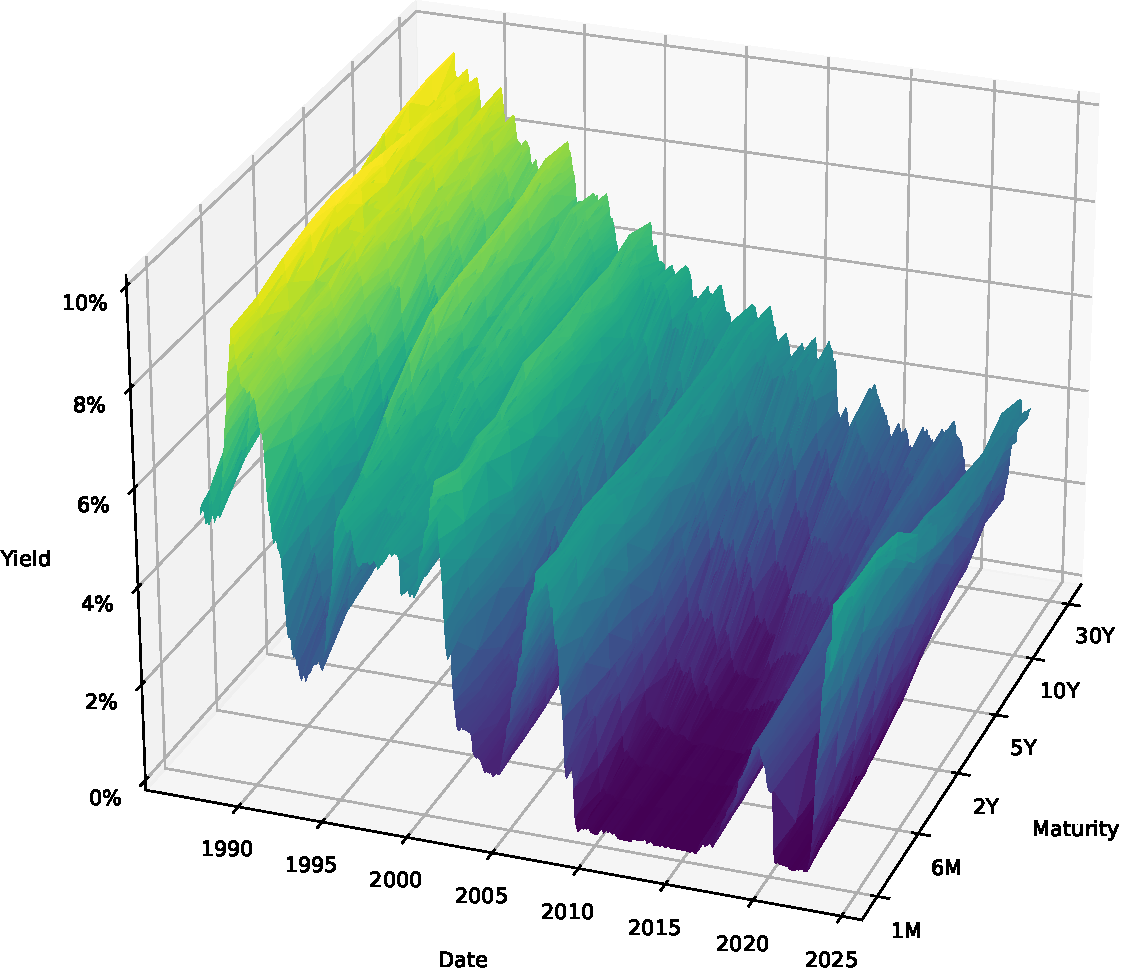
\includegraphics[width=0.75\linewidth]{Figures/fed_rates.pdf}
    \end{center}
   \caption[3D plot of the yield on US treasuries of various maturities over time]{A 3D plot of the yield on US treasuries of various maturities over time. } 
    \label{fig:US_yield_curve} 
\end{figure} 

One key intrinsic factor that can influence the yield of a bond is its maturity, representing the length of time before the principal must be repaid. Under normal market conditions, long-term fixed-income securities, such as 20-year bonds, typically provide higher returns than their short-term counterparts, such as 2-year bonds. This is primarily due to the greater uncertainty associated with longer-term securities, especially concerning potential fluctuations in future interest rates. For a set of equivalent bonds differing only based on their maturity length, the yield is expected to interpolate smoothly at any given time, forming the so-called yield curve. \Cref{fig:US_yield_curve} demonstrates how the yield curve for US treasuries has varied over the past 35 years.

For bonds issued by other entities, such as state authorities, numerous intrinsic factors other than maturity may affect the yield. These include the credit rating of the issuer, the tax exemption status, and, particularly relevant to green bonds, the Environmental, Social and Governance (ESG) impact of the funded project. In this case study, we frame the problem of estimating unknown yields as a multiway graph signal processing task. Specifically, we categorise the bonds based on several factors likely to influence the yield, such that each bond can be associated with a node on a four-dimensional Cartesian product graph. In particular, we take into account the following factors, each of which forms the basis of one of the factor graphs. 

\begin{enumerate}
    \item \textit{Use of funds}. Each bond in our dataset was associated with a project category (such as water, pollution or power) and sub-category (such as waste management, habitat conservation, or solar farms). We used this information to construct a tree graph, beginning with a root node, and branching into category and sub-category nodes. The resulting tree, comprising a total of 161 nodes, is visualised in \cref{fig:green_bond_graph}. Each bond can then be associated with a specific leaf node based on their particular project category.
    \item \textit{Credit rating}. Each bond also had an assigned credit rating associated with the issuer, designated by a ratings agency. These ratings range from the highest possible, ``AAA", to the lowest in our dataset, ``BBB+", giving a total of eight categories. Since these ratings have a natural order, they can be represented using a simple chain graph.
    \item \textit{Maturity}. Each bond has a fixed period from its issue date to the date of maturity. Unlike treasury bonds, the green bonds we considered did not necessarily have standard maturity lengths. We thus categorised each bond by the length of this period, sorted into eight different bins, with edges corresponding to 0, 1, 2, 5, 10, 20, 30, 40 and 50 years. As with credit rating, the natural order enables us to represent this with a chain graph.
    \item \textit{Tax status}. Each bond also has an associated tax status. This includes information about whether the bond was taxed at the federal and state level, as well as certain other provisions such as special exemptions for specific institutions. We represented tax status as a network, where any two codes were connected if they shared at least one property in common. Further information on the possible green bond tax statuses is presented in \cref{table:student}, and the graph we used to connect them is depicted in \cref{fig:tax_graph}.
    \end{enumerate}

\begin{figure}[t]  
    \begin{center}
        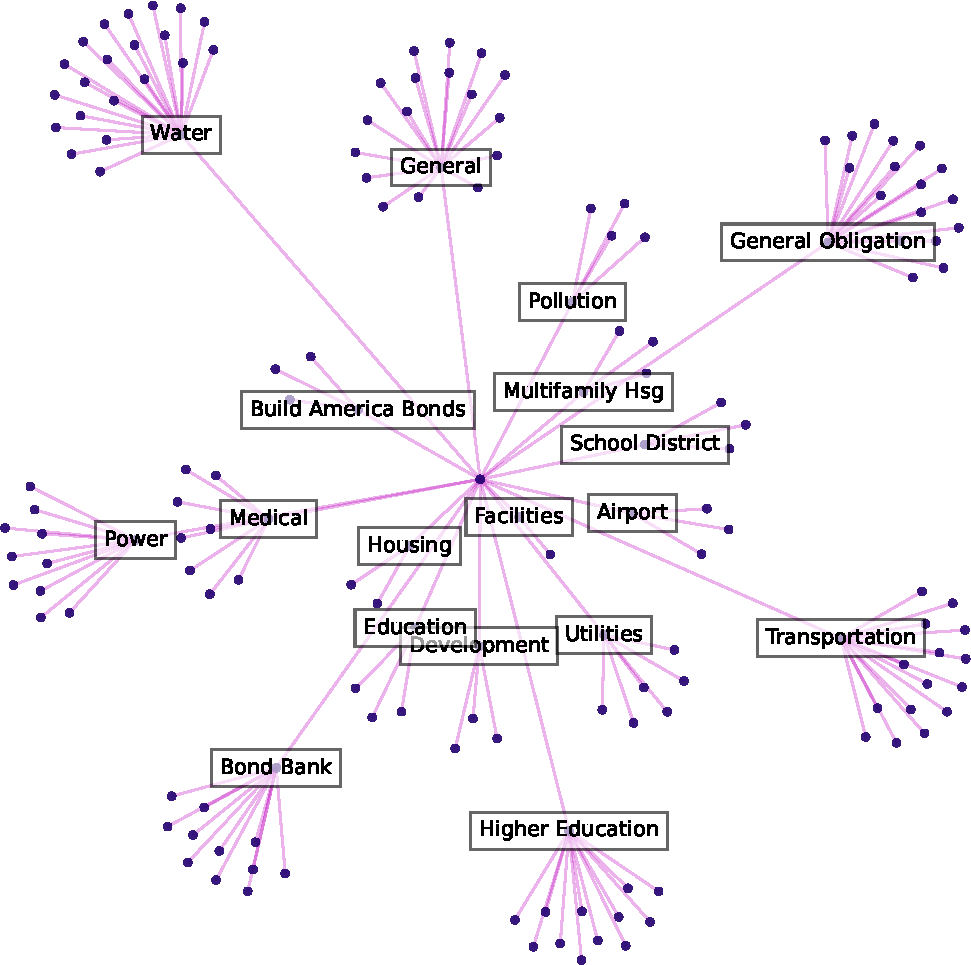
\includegraphics[width=0.8\linewidth]{Figures/bond_graph.pdf}
    \end{center}
   \caption[Graph categorising green bonds based on sector]{A representation of the graph used for categorising municipal green bonds based on the sector of the project. } 
    \label{fig:green_bond_graph}
    \vspace{1.5cm}
\end{figure} 

\begin{table}[t]
    \centering
    \def\arraystretch{1.5}
    \begin{tabular}{l p{9cm}}
        \toprule
        \textbf{Tax Status} & \textbf{Description} \\ 
        \midrule
        Fed \& St Tax-Exempt & Exempt from tax at both the federal and state level.  \\ 
        Fed Taxable/St Tax-Exempt & Taxable at the federal level, exempt at the state level.  \\ 
        Fed Tax-Exempt/St Taxable & Exempt at the federal level, taxable at the state level. \\ 
        Fed BQ/St Tax-Exempt & ``Bank Qualified'' (special provisions for large banks) at the federal level, exempt at the state level.  \\ 
        Fed Tax-Exempt & Exempt at the federal level, no information about the state level. \\ 
        AMT/St Tax-Exempt & ``Alternate Minimum Tax'' (special provision removing certain tax deductions) at the federal level, exempt at the state level. \\ 
        Fed Taxable/St Taxable & Taxable at both the federal and state level. \\ 
        \bottomrule
       \end{tabular}
        \caption[Information on the tax status of green bonds]{Further information on the possible tax status of the green bonds used in this case study.}
        \label{table:student}
\end{table}

\begin{figure}[b]  
    \begin{center}
        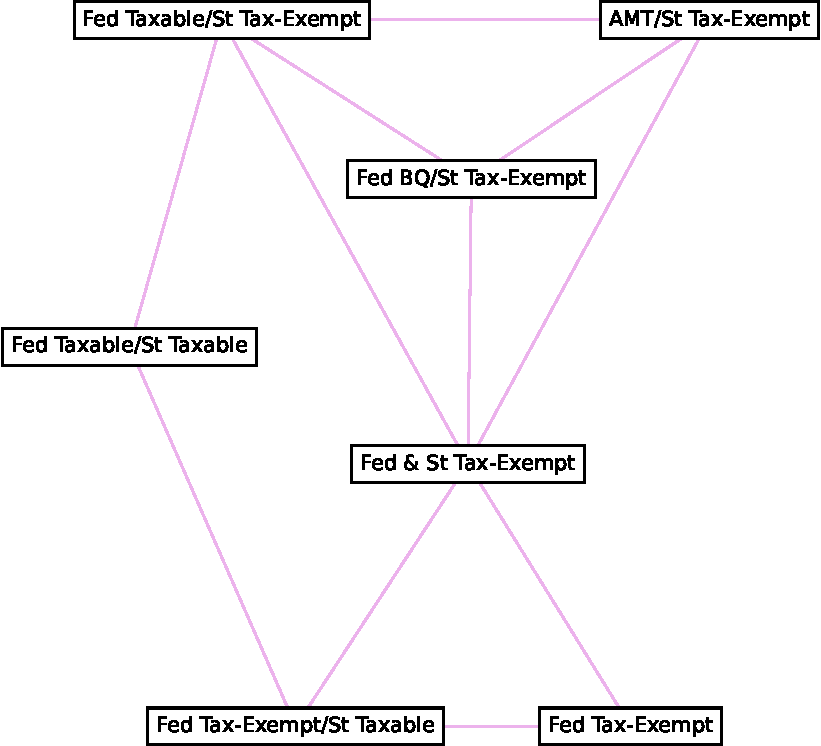
\includegraphics[width=0.66\linewidth]{Figures/tax_graph.pdf}
    \end{center}
   \caption[Graph categorising green bonds based on tax status]{A representation of the graph used for categorising municipal green bonds based on the associated tax status. Two different statuses are linked via an edge if they share at least one property in common. } 
    \label{fig:tax_graph}
\end{figure} 


\newpage 

\phantom{blabla}

\newpage


Given these factors, each bond could be associated with a particular four-dimensional coordinate: use of funds, credit rating, maturity, and tax status. With the inclusion of a time coordinate, encompassing weekly data from June 2018 to March 2023, the resulting input tensor $\Yt$ had five distinct axes, with an overall shape of $(429, 161, 8, 8, 7)$. For the KGR model, this can be interpreted as $T=429$ repeated measurements of a 4-dimensional multiway graph signal, and for the GSR model, it can be regarded as a single measurement of a 5-dimensional graph signal, with time also represented by a chain graph. \Cref{fig:bond_tensor} provides a visual representation of the tensor signal, $\Yt$, utilised in this application.

\begin{figure}[t] 
    \begin{center}
        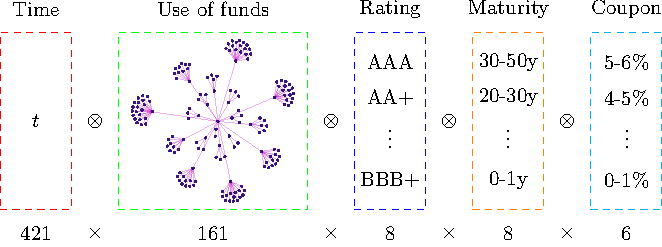
\includegraphics[width=0.9\linewidth]{Figures/bond_tensor.pdf}
    \end{center}
   \caption[A visualisation of the tensor coordinates used in the greed bond application]{A visualisation of the tensor coordinates used in this application. Rating, maturity and coupon are all represented by a chain graph, while category is a tree graph as described above.} 
    \label{fig:bond_tensor}
\end{figure} 

For many specific tensor coordinates, no bond yield existed, and as such the tensor $\Yt$ was very sparse. This could be due to the fact that the bond was not trading at this particular time, or because no bond ever existed with these particular characteristics. Moreover, since the parent nodes in the graph representing the use of funds are in a sense ``artificial" - serving solely to create the tree structure - no realised yield could possibly exist there. Under the framework developed in this thesis, this does not present a problem, since we can simply allocate these coordinates as containing missing data, as specified by the binary sensing tensor $\St$. 

Additionally, there were certain bonds that shared identical characteristics, i.e., the same use of funds, rating, maturity, and tax status. In these instances, we simply selected the bond with the longest available history and randomly broke ties. In total, we used 829 bonds (out of a theoretically possible $161 \times 8 \times 8 \times 7 = 72,128$). As many bonds did not span the total 429 weeks, this left a total missingness of $m=99.27\%$.

As previously noted, one model we employ in this case study to predict the yields is Kernel Graph Regression. This necessitates, in addition to the input tensor $\Yt$ and the sensing tensor $\St$, a matrix of explanatory variables $\X$ with shape $(T, M)$. Here, we use the treasury yields over 11 different maturities, along with core inflation, the Federal Reserve fund rate, and a simple linear variable $t$ ranging from -1 to 1, totalling $M=14$ explanatory variables. This data was obtained from the FRED API \citep{FRED2023}.


\begin{table*}[t] 
    \centering
    \def\arraystretch{1.5} 
    \begin{tabular}{@{}ccccccccc}
    \toprule
    & \multicolumn{2}{c}{Training} & \phantom{abc} & \multicolumn{2}{c}{Validation} & \phantom{abc} & \multicolumn{2}{c}{Test} \\
    \cmidrule{2-3} \cmidrule{5-6} \cmidrule{8-9}
    & MSE  & $R^2$  &&  MSE  & $R^2$ &&  MSE  & $R^2$  \\ \midrule \rule{0pt}{1cm}

    GSR & 0.263 & 0.846 && 0.332 & 0.819 && 0.319 & 0.823 \\ \rule{0pt}{6ex}
    
    KGR & 0.266 & 0.845 &&  0.333 & 0.820 && 0.317 & 0.824 \\\rule{0pt}{6ex}
    
    Ridge & 0.387 & 0.775 && 0.501 & 0.729 && 0.497 & 0.725 \\ \rule{0pt}{6ex}
    
    Lasso &  0.424 & 0.753 && 0.482 & 0.739 && 0.506 & 0.720 \\[0.5cm] 

    \bottomrule 
    \end{tabular}
    \caption[Results for bond yield experiments]{The Mean Square Error (MSE) and $R^2$ statistic from the bond yield experiment are shown for both GSR and KGR. Results are reported on the training set, the validation set, and the test set. }
    \label{tab:bond_yield_results} 
\end{table*}

Our experiment proceeded as follows. Firstly, we randomly divided the 829 bonds into a training, validation, and test set in an 80:10:10 ratio. We then trained the GSR and KGR models on the training set, using the validation set to select the optimal hyperparameters, identified using an optimisation algorithm based on the Nelder-Mead method \citep{Gao2012}. In addition, we evaluated two standard linear regression techniques, namely Ridge and Lasso \citep{Murphy2012}. In these scenarios, the yield at each moment in time for each bond was modelled as a linear combination of a constant term, the features comprising the matrix $\X$, and a one-hot encoding of each of the bond descriptors (use of funds, rating, etc). This resulted in $1 + 14 + 159 + 8 + 8 + 7 = 197$ explanatory variables for each yield. The regularisation parameter for the Ridge and Lasso models was also selected on the validation set using a straightforward line search.

The results from the experiment can be found in \cref{tab:bond_yield_results}. As can be observed, the GSR and KGR methods attain similar performance to each other, consistently outperforming the Ridge and Lasso techniques. Both also display a Mean Square Error (MSE) and $R^2$ statistic that remains relatively constant across the training, validation, and test sets, suggesting that overfitting has largely been avoided. \Cref{fig:bond_yield_predictions} showcases the output of both GSR and KGR compared with the ground truth, for nine randomly selected bonds from the test set. We can observe that both GSR and KGR make broadly similar predictions, which often correlate closely with the ground truth. However, there are instances where the predictions clearly systematically under or overestimate the yield, for example in the upper middle, middle left, and lower middle plots. This may indicate there was hidden information about this bond not accounted for in our explanatory variables. Further investigation into the reasons for these deviations would be valuable.

\begin{figure}[t]  
    \begin{center}
        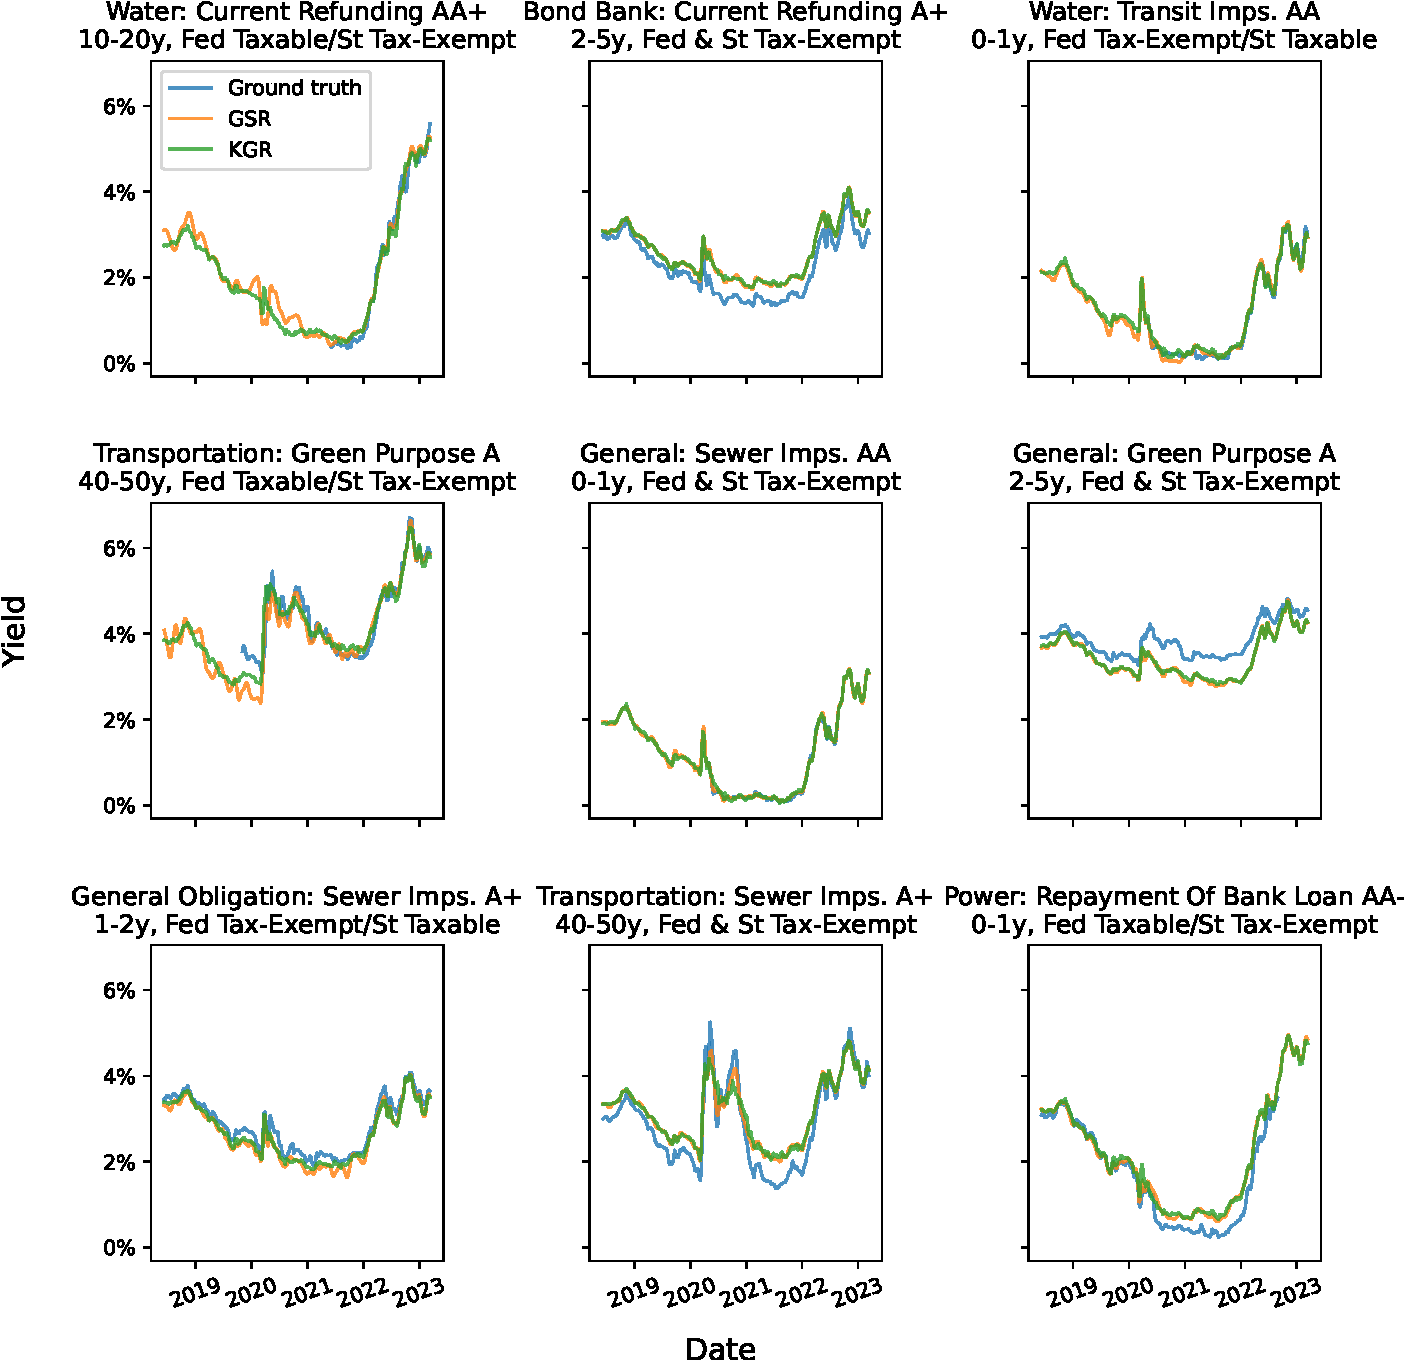
\includegraphics[width=\linewidth]{Figures/bond_yield_predictions.pdf}
    \end{center}
   \caption[The output of the KGR and GSR algorithms on several green bonds from the test set]{The predicted yield is shown from the KGR and GSR algorithms as compared to the ground truth on a set of green bonds taken from the test set. } 
    \label{fig:bond_yield_predictions}
\end{figure} 



\section{Conclusions}

In this chapter we have been concerned with generalising several graph signal processing methods to the $d$-dimensional tensor setting. In \cref{sec:dd_gsp}, we discussed how the Cartesian product can be generalised to include more than two factor graphs, resulting in tensor-valued multiway graph signals. In \cref{sec:GSP_dd,sec:fast_kron_dd}, we reviewed how GSP techniques such as the GFT can be understood for $d$-dimensional signals, and introduced the concept of a general anisotropic graph filter. We also discussed how $d$-dimensional Kronecker products can be efficiently computed and presented the PyKronecker software library for this purpose \citep{Antonian2023}.

In \cref{sec:tensor_gsr}, we reexamined the Graph Signal Reconstruction model developed in \cref{chap:gsr_2d}, generalising it to $d$ dimensions. This necessitated a fresh look at the SIM and CGM methods previously developed to make them applicable for this setting. Next, in \cref{sec:kgr_dd,sec:rnc_dd} respectively we took the Kernel Graph Regression and Regression with Network Cohesion techniques, which were developed in \cref{chap:kgr_rnc_2d}, and generalised them for the multiway case. Finally, in \cref{sec:green_bonds}, we showed how the multiway KGR and GSR methods could be applied to the problem of predicting the yield of novel green bonds in a time series application. In particular, we showed that both GSR and KGR could achieve good performance, significantly out-performing the standard techniques of Ridge and Lasso regression. 





\chapter{Regression and Reconstruction with Tensor-Valued
Muliway Graph Signals}

\lhead{Chapter 6. \emph{Regression and Reconstruction with
Muliway Graph Signals}}

\label{chap:nd_gsp}


Multiway Graph Signal Processing (MWGSP) is an emerging framework for analysing signals with multiple distinct axes (or `ways'), where the relation between elements within each axis is described by a graph topology \citep{Stanley2020}. For example, consider an fMRI experiment where cerebral blood flow is measured at a set of 3D voxels across time, for multiple subjects, in response to various stimuli. This dataset could be modelled as a six-way graph signal with the three spatial coordinates and the one time coordinate forming a four-way hypergrid graph, the subjects forming a graph based on characteristics, and the stimuli forming a graph based on similarity \citep{Cichocki2015}. A visual depiction of this is given in \cref{fig:fMRI_diagram}. 
 
\vspace{1.5cm}

\begin{figure}[h] 
    \begin{center}
        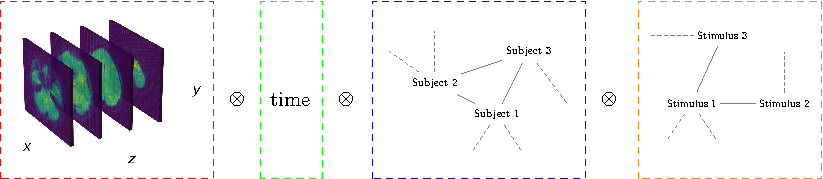
\includegraphics[width=\linewidth]{Figures/fMRI_Digaram.pdf}
    \end{center}
   \caption[Graphical depiction of an order-3 tensor]{Graphical depiction of a six-way graph signal originating from a hypothetical fMRI experiment. } 
    \label{fig:fMRI_diagram}
\end{figure} 


\begin{figure}[b] 
    \begin{center}
        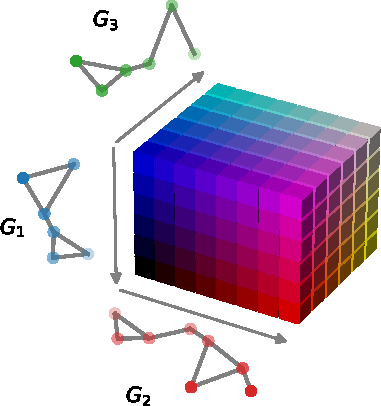
\includegraphics[width=0.4\linewidth]{Figures/coloured_tensor.pdf}
    \end{center}
   \caption[Graphical depiction of an order-3 tensor]{Graphical depiction of an order-3 tensor signal with graphs underlying each axis. } 
    \label{fig:coloured_tensor}
\end{figure}  

The goal of this chapter is to extend the methods developed in \cref{chap:gsr_2d,chap:kgr_rnc_2d} such that they can accommodate multiway graph signals. In particular, Graph Signal Reconstruction (GSR), Kernel Graph Regression (KGR) and Regression with Network Cohesion (RNC) can all be understood as special two-dimensional cases of their more general and versatile MWGSP counterparts. In this chapter, we translate all three models into a their $d$-dimensional form, and demonstrate how to solve efficiently for the posterior mean. This framework forms the basis for the models developed in \cref{chap:variance,chap:binary}. 


Multiway signals are represented using tensors, which are often conceptualised as $d$-dimensional arrays. Tensor algebra is well-established in fields such as physics and mechanics \citep{Renteln2013}, however it is less widespread in the graph signal processing community. As such, the first section of this chapter sets out some conceptual and notational standards for tensors. In MWGSP, each axis of the tensor has an underlying graph topology, with each factor graph linked together in a $d$-dimensional Cartesian product. \Cref{fig:coloured_tensor} gives some visual intuition for this with an order-3 tensor signal.  


We begin \cref{sec:dd_gsp} by defining the Cartesian product of more than two graphs, and discuss the algebraic and spectral structure of the resultant objects. Next, we cover the tensor representation of multiway graph signals and give the general definition of a graph-spectral operators in $d$-dimensions. We also discuss issues surrounding computational efficiency and how the so called `vec-trick' utilised in prior chapters can be generalised to the tensor setting. In \cref{sec:tensor_gsr}, we begin the core contributions of this chapter by generalising Bayesian GSR as defined in \cref{chap:gsr_2d} to the multiway GSP setting. This necessitates an updated version of the SIM and CGM to accommodate tensor-valued data in arbitrary dimensions, which we give in \cref{sec:SIM_dd,sec:CGM_dd}. Next, in \cref{sec:kgr_dd}, we generalise KGR for the non-parametric prediction of multiway graph signals as a function of exogenous variables. Finally, in \cref{sec:rnc_dd}, we the generalise RNC as defined in \cref{sec:rnc_mdp} in much the same way.  



\section{Multiway Graph Signal Processing}

\label{sec:dd_gsp}

\subsection{The Cartesian product of more than two graphs}

In \cref{sec:graph_products_defined} we gave the general definition of a product between two graphs and highlighted four standard examples, namely the Cartesian, direct, strong and lexicographic products. Each of these product types can be straightforwardly extended to more than two factor graphs by applying their respective definition recursively. For example, consider the Cartesian product between graphs $\mathcal{G}_A = \{\mathcal{V}_A, \mathcal{E}_A\}$, $\mathcal{G}_B = \{\mathcal{V}_B, \mathcal{E}_B\}$ and $\mathcal{G}_C = \{\mathcal{V}_C, \mathcal{E}_C\}$ where $|\mathcal{V}_A| = A$, $|\mathcal{V}_B| = B$ and $|\mathcal{V}_C| = C$. This can be written as 

\begin{equation}
    \mathcal{G} \; = \; \mathcal{G}_A \, \square \; \mathcal{G}_B \, \square \; \mathcal{G}_C \; = \; \{\mathcal{V}, \, \mathcal{E}\}
\end{equation}

The new vertex set, $\mathcal{V}$, is given by the Cartesian product of the individual vertex sets, arranged in lexicographic order. 

\begin{equation}
    \mathcal{V} = \mathcal{V}_A \times \mathcal{V}_B \times \mathcal{V}_C = \{(a, \, b, \, c) \in \mathbb{N}^3 \, | \, a \leq A, \; b \leq B, \text{and} \;  c \leq C\}
\end{equation}

The new edge set, $\mathcal{E}$, is given by recursively applying conditions 1 and 7 from, \cref{sec:graph_products_defined} to the new node set. In particular, any two nodes $(a, \, b, \, c)$ and $(a', b', c')$ are connected in $\mathcal{E}$ if they satisfy any of the following three conditions. 

\vspace{0.5cm}

\begin{table}[h]
    \def\arraystretch{1.5}
    \centering
    \begin{tabular}{lclclc}
        1. & $[a, \, a'] \in \mathcal{E}_A$    & and & $b = b'$  & and & $c = c'$             \\
        2. & $a = a'$    & and & $[b, \, b'] \in \mathcal{E}_B$   & and & $c = c'$             \\
        3. & $a = a'$    & and & $b = b'$  & and & $[c, \, c'] \in \mathcal{E}_C$              \\
    \end{tabular}
\end{table}


\begin{figure}[t]
    \begin{center}
        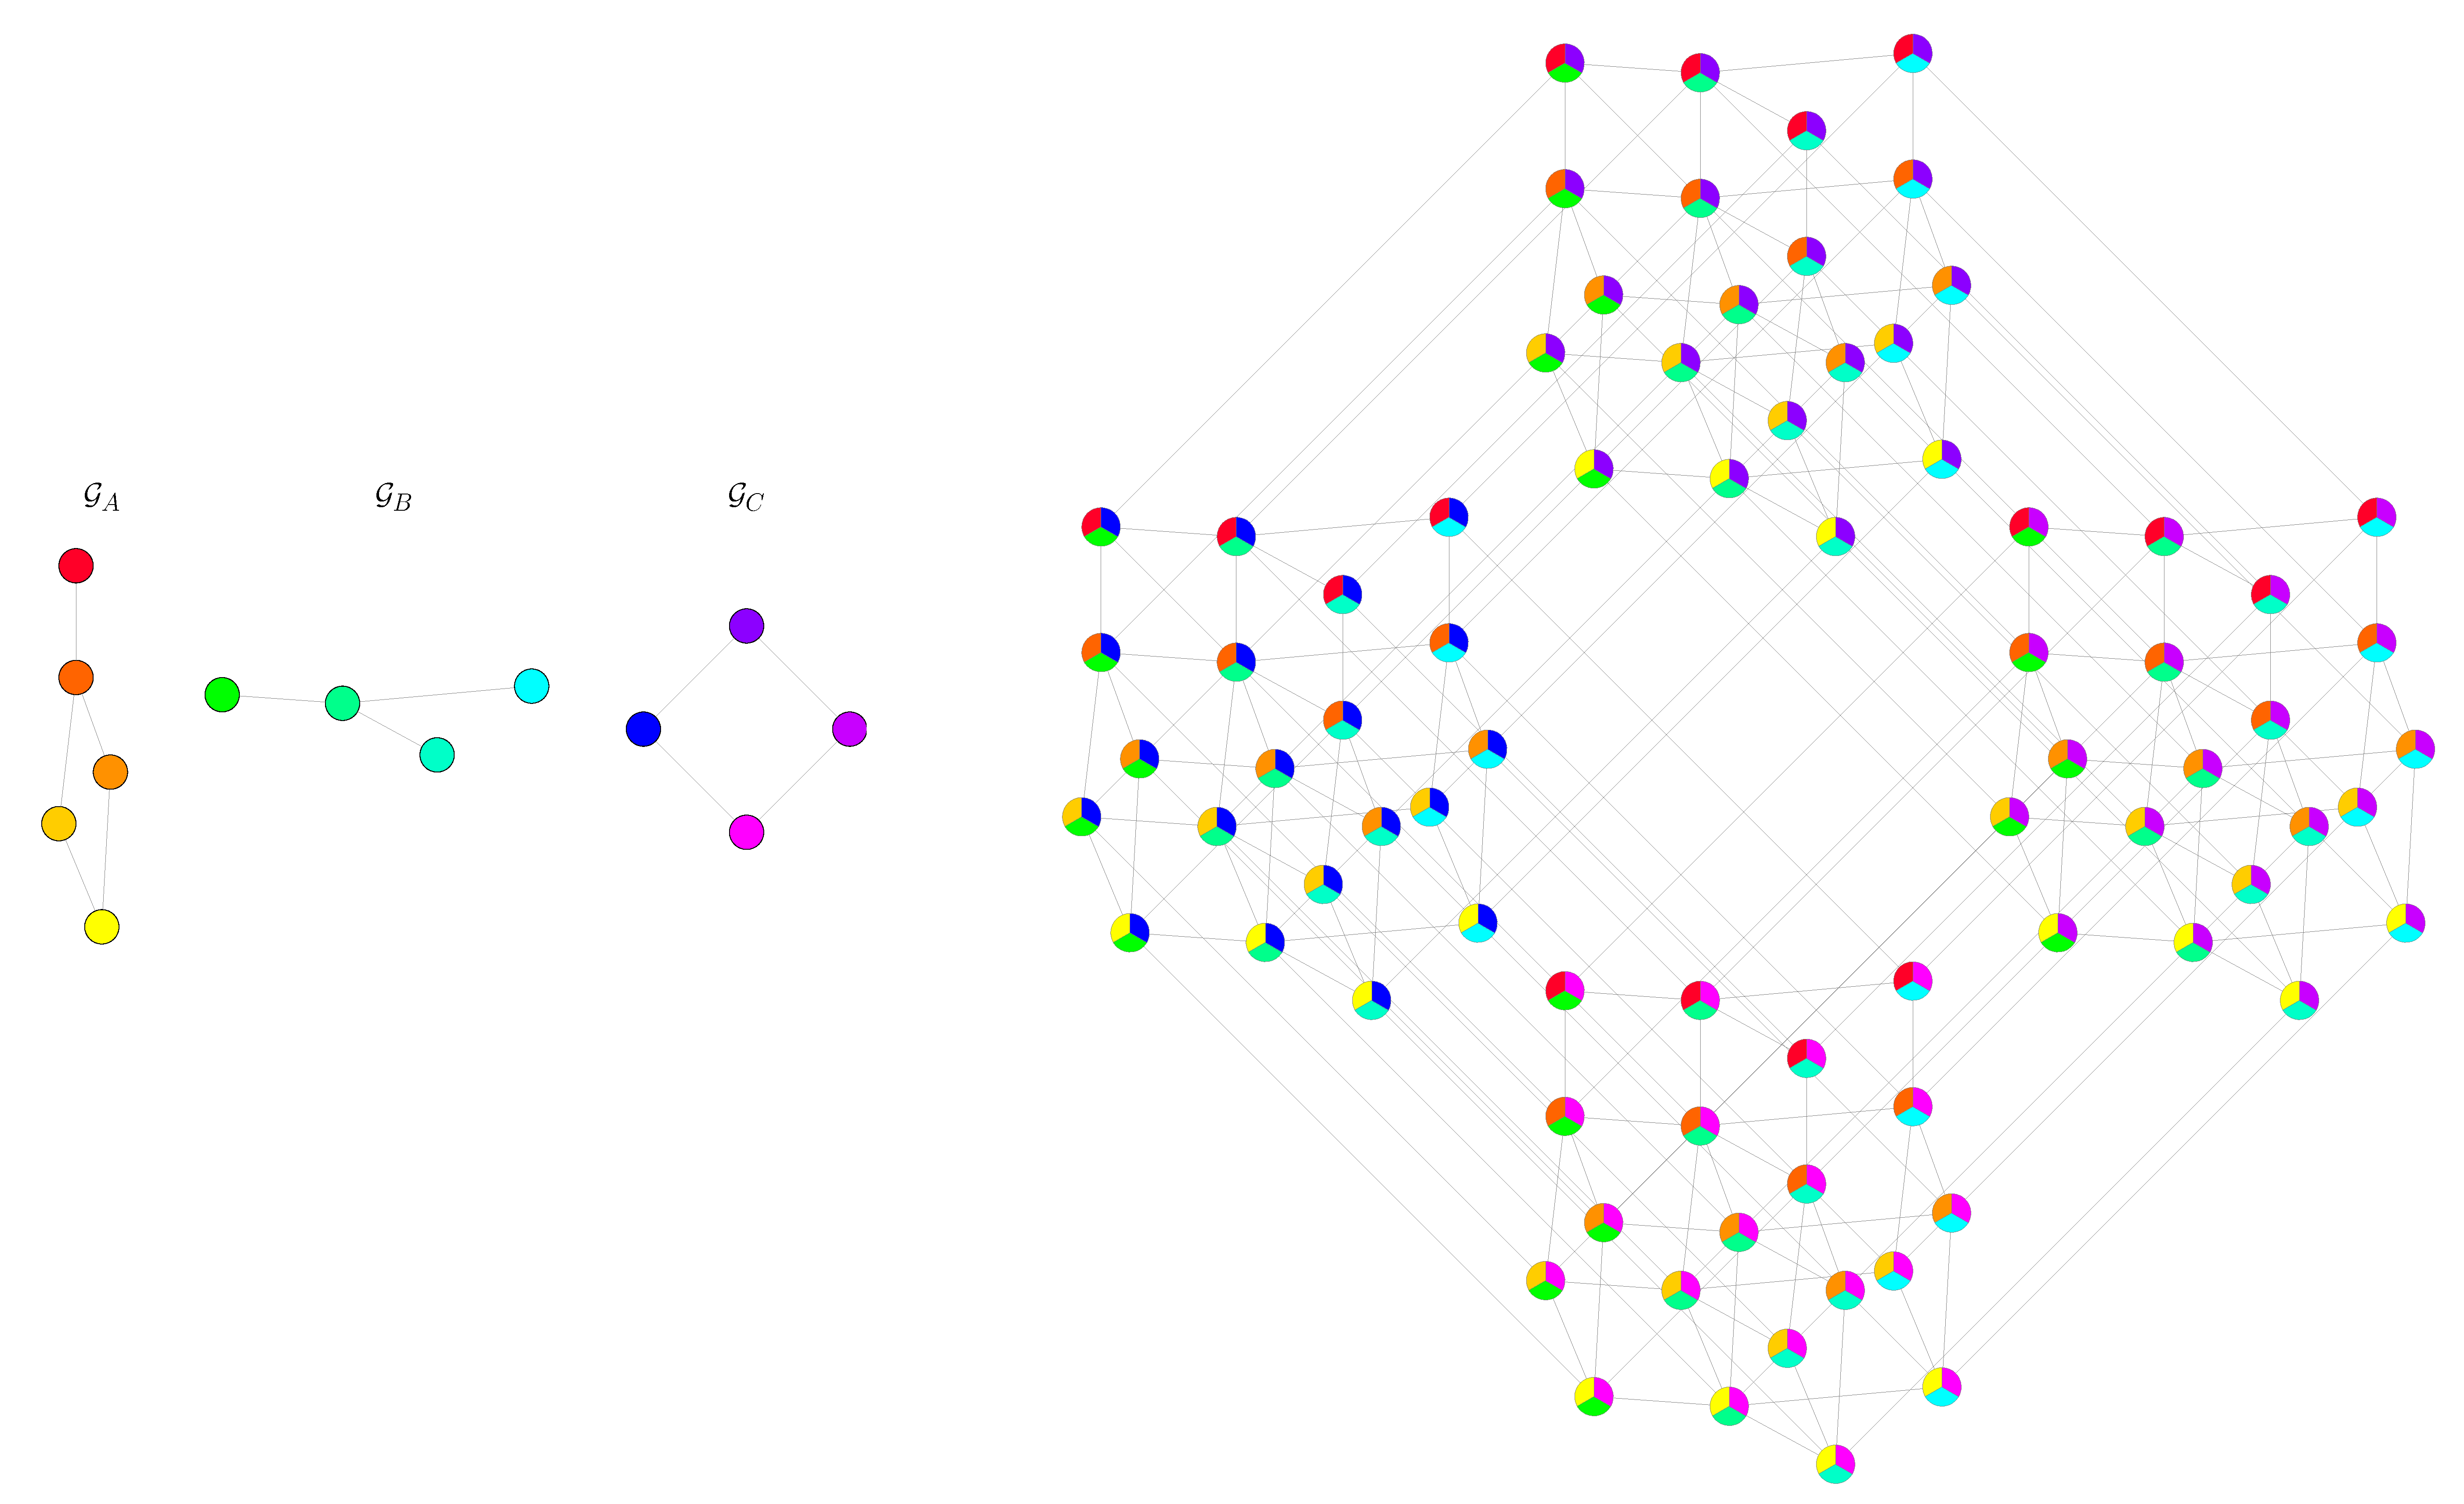
\includegraphics[width=\linewidth]{Figures/3D_CPG.pdf}
    \end{center}
    \caption[Graphical depiction of a 3D Cartesian product graph]{Graphical depiction of a 3D Cartesian product graph}
    \label{fig:3D_CPG}
\end{figure}

\Cref{fig:3D_CPG} gives a visual representation of a Cartesian product graph formed from three simple factor graphs. Notice that the size of the new vertex and edge set both grow very quickly. In particular, 

$$
|\mathcal{V}| = |\mathcal{V}_A| |\mathcal{V}_B| |\mathcal{V}_C| \aand |\mathcal{E}| =  |\mathcal{E}_A| |\mathcal{V}_B| |\mathcal{V}_C| + |\mathcal{V}_A| |\mathcal{E}_B| |\mathcal{V}_C| + |\mathcal{V}_A| |\mathcal{V}_B| |\mathcal{E}_C|
$$

Happily, the adjacency matrix of a Cartesian product graph $\A$ has a straightforward representation in terms of the factor adjacency matrices (here $\A_A$, $\A_B$ and $\A_C$). Specifically, it is given by their Kronecker sum. 

\begin{align}
    \A &= \A_A \oplus \A_B \oplus \A_C \notag \\
    &= \A_A \otimes \I_B \otimes \I_C  + \I_A \otimes \A_B \otimes \I_C + \I_A \otimes \I_B \otimes \A_C
\end{align}

In general, we can consider the Cartesian product of $d$ factor graphs with adjacency matrices denoted as $\A^{(1)} \in \R^{N_1 \times N_2}, \A^{(2)} \in \R^{N_2 \times N_2}, \dots \A^{(d)} \in \R^{N_d \times N_d}$. The full adjacency matrix will have size $N \times N$, where $N = \prod N_i$, and is given by  

\begin{alignat}{4}
    \A = \A^{(1)} & \oplus \A^{(2)} & \oplus \;\; ... \;\; & \oplus \A^{(d)} \notag \\[0.1cm]
    = \A^{(1)} & \otimes \I_{N_2} & \otimes \;\; ... \;\; & \otimes \I_{N_d} +  \notag \\[0.1cm]
    \I_{N_1} & \otimes \A^{(2)} & \otimes \;\; ... \;\; & \otimes \I_{N_d} + \;\; \ldots \;\; +  \notag \\[0.1cm]
    \I_{N_1} & \otimes \I_{N_2} & \otimes \;\; ... \;\; & \otimes \A^{(d)}  
\end{alignat}
    
This can be written compactly as 

\begin{equation}
    \A = \bigoplus_{i=1}^d  \A^{(i)}
\end{equation}

Similarly, the Laplacian of the product graph, $\LL$, can be written as the Kronecker sum of the individual factor graph Laplacians $\LL^{(i)}$. 

\begin{equation}
    \LL = \bigoplus_{i=1}^d  \LL^{(i)}
\end{equation}

We can perform eigendecomposition on each of the individual graph Laplacians as follows. 

\begin{equation}
    \LL^{(i)} = \U^{\,(i)} \LAM^{(i)} (\U^{\,(i)})^\top
\end{equation}

\noindent where $ \U^{(i)}$ is an orthogonal matrix such that each column is an eigenvector of $\LL^{(i)}$, and $\LAM^{(i)}$ is a diagonal matrix containing the corresponding eigenvalues, which are typically listed in ascending order. 

$$
\LAM^{(i)} = 
\begin{bmatrix}
    \lambda_1^{(i)}, &                 &        &                 \\
                     & \lambda_2^{(i)} &        &                 \\
                     &                 & \ddots &                 \\
                     &                 &        & \lambda_{N_i}^{(i)} \\
\end{bmatrix}
$$

Given this, the Laplacian of the product graph can be decomposed as follows. 

\begin{align}
    \LL &= \bigoplus_{i=1}^d \U^{\,(i)} \LAM^{(i)} (\U^{\,(i)})^\top \notag \\[0.2cm]
    &= \left( \bigotimes_{i=1}^d  \U^{\,(i)} \right) \left(\bigoplus_{i=1}^d \LAM^{(i)} \right) \left(\bigotimes_{i=1}^d  \U^{\,(i)} \right)^\top \notag \\[0.2cm]
    &= \U \LAM \U^\top 
\end{align}

\noindent where 

\begin{equation}
    \label{eq:U_LAM_def}
    \U =  \bigotimes_{i=1}^d  \U^{\,(i)} , \quad \text{and} \quad \LAM =  \bigoplus_{i=1}^d \LAM^{(i)}
\end{equation}


Here, we have used the notation $\bigotimes_{i=1}^d  \U^{\,(i)}$ to denote the chained Kronecker product of matrices $\{\U^{\,(i)}  \}$. 

\subsection{Representing \textit{d}-dimensional graph signals}

Since each node in a $d$-dimensional product graph is specified by $d$ independent indices, a signal $\Yt$ existing over the nodes has a natural representation as a tensor of order $d$. One way to conceptualise a $d$-dimensional tensor signal is as a multi-dimensional array with $d$ independent axes. If the $i$-th factor graph has $N_i$ vertices, then $\Yt$ will be of shape $(N_1, \, N_2 , ... N_d)$. An individual element of this tensor signal can be specified via a vector index $\nn = [n_1,\, n_2,\, ...,\, n_d]$, where $1\leq n_i \leq N_i$.

Alternatively, signals can be represented as a vector of length $N = \prod N_i$. This is essential if we are to interpret the $\otimes$ symbol strictly as a Kronecker product, rather than a tensor or outer product. Under the Kronecker interpretation, the chained use of $\otimes$ used in expressions such as \cref{eq:U_LAM_def} results in matrices of shape $N \times N$, providing a linear map from $\R^{N} \rightarrow \R^{N}$. Therefore, for an operator to act on a tensor graph signal $\Yt \in \R^{N_1 \times N_2 \times ... \times N_d}$, we need a method of mapping tensors with shape $(N_1, \, N_2 , ... N_d)$ to vectors of length $N$. In order for this vectorisation process to be consistent with the operators, it should result in a vectors whose elements are arranged in lexicographic order. In some fields, this is referred to as \textit{row-major} vectorisation since, in the case of an order-2 tensor, the index representing the row varies before the column index. In the following, we symbolise this operation mathematically as $\vecrm{\cdot}: \R^{N_1 \times N_2 \times ... \times N_d} \rightarrow \R^N$, and its reverse operation as $\tenrm{\cdot}: \R^N \rightarrow \R^{N_1 \times N_2 \times ... \times N_d}$. We use the `RM' subscript to indicate explicitly that this process is occurring in row-major order, since the standard $\vecc{\cdot}$ function defined for matrices is most commonly assumed to act in column-major order.  

In the following, we use bold lower-case symbols (e.g. $\y$) to indicate graph signals existing in their vector form, and bold upper-case calligraphic symbols (e.g. $\Yt$) to indicate graph signals in their multi-dimensional array form. That is, 

\begin{align*}
    \y = \vecrm{\Yt} \quad \implies \quad \Yt  = \tenrm{\y}
\end{align*}

\Cref{fig:ten_to_vec} shows gives a visual summary of the process of converting between these two representations for an order-3 tensor. 


\begin{figure}[t]
    \begin{center}
        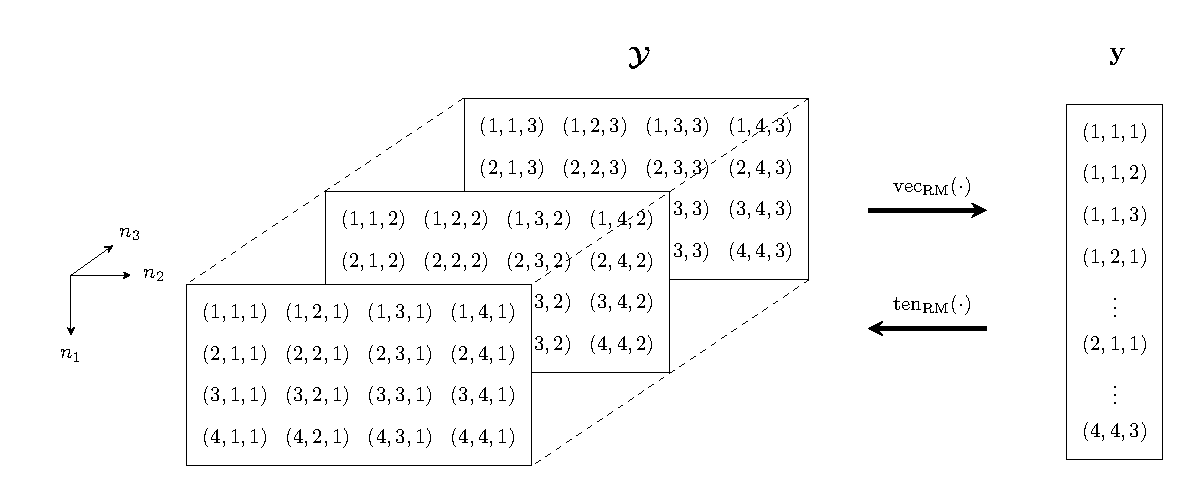
\includegraphics[width=\linewidth]{Figures/Tensor_Digaram.pdf}    
    \end{center}
    \caption[Conversion between a multidimensional array and a vector]{A graphical depiction of the process of converting an order-3 tensor between its multidimensional array and vector form in row-major order. Note that the elements in the vectorised signal are lexicographically ordered. }
    \label{fig:ten_to_vec}
\end{figure}


To calculate the vector index $k$ which a tensor element with index $\nn = [n_1,\, n_2,\, ...,\, n_d]$ is mapped to in row-major order, we can apply the following formula.  

\begin{equation}
    \label{eq:vec}
    k = 1 + \sum_{i=1}^d \Big( \prod_{j=i+1}^d N_j \Big) \, (n_i - 1)
\end{equation}

(Note the $\pm1$ disappear when indexing begins from zero). The reverse operation, i.e. mapping a vector element index $k$ to a tensor index $\nn$ can be achieved by running the algorithm \hyperlink{vectoten}{\textbf{3}}. 


\begin{algorithm}[t]
    \hypertarget{vectoten}{}
    \label{al:vectoten}
    \caption{Mapping a vector element to a tensor element in row major order}
    \begin{algorithmic}
    \vspace{0.15cm}
    \Require{The target vector element $k$} 
    \vspace{0.1cm}
    \Require{The shape of the output tensor $(N_1, N_2, ..., N_d)$} 
    \vspace{0.25cm}
    \State{$k \leftarrow  k - 1$}
    \vspace{0.25cm}
    \For{$i$ \textbf{from} $d$ \textbf{to} 1}
    \vspace{0.25cm}
    \State{$n_i \leftarrow  k \mod N_i$}
    \vspace{0.15cm}
    \State{$k \leftarrow \lfloor k / N_i \rfloor$} 
    \vspace{0.15cm}
    \EndFor
    \vspace{0.25cm}
    \Ensure{$(n_1 + 1, n_2 + 1, ..., n_d + 1)$}
    \end{algorithmic}
\end{algorithm}



Given these two operations, two arrays of any consistent shape can be mapped between one another by first vectorising according to \cref{eq:vec}, and then converting to a tensor using the given algorithm.



\subsection{GSP in \textit{d}-dimensions}



Consider a graph signal $\Yt \in \R^{N_1 \times N_2 \times ... \times N_d}$ represented in its tensor form. In direct analogy to the two dimensional case given in \cref{eq:GFT_2d,eq:IGFT_2d}, we can define the Graph Fourier Transform (GFT) and its corresponding inverse (IGFT) of this signal as follows. 

\begin{alignat}{2}
\label{eq:gft_nd}
    \text{GFT}(\Yt) & = \tenrm{\U^\top \y} && = \tenrm{\left(  \bigotimes_{i=1}^d  \U^{\,(i)} \right)^\top \vecrm{\Yt} } \\
\label{eq:igft_nd}
    \text{IGFT}(\Yt) & = \tenrm{\U \y} && = \tenrm{\left(  \bigotimes_{i=1}^d  \U^{\,(i)} \right) \vecrm{\Yt} }
\end{alignat}

The concept of a graph filter for signals defined on a Cartesian product graph follows naturally from this definition. Just as in the one and two-dimensional case, a graph filter is constructed by first taking the GFT of a signal, then applying some scaling function to each spectral component, then transforming back into the vertex domain via the IGFT. In the simplest case, we can consider an isotropic graph filter function $g(\lambda, \beta)$, such as one of those defined in \cref{tab:iso_filters}. A filter $\HH$, defined to act on a vectorised graph signal, can be represented as an $N \times N$ matrix, constructed as follows. 


\begin{align}
    \label{eq:H_def_dd}
    \HH &= \left( \bigotimes_{i=1}^d  \U^{\,(i)} \right) g\left(\bigoplus_{i=1}^d \LAM^{(i)}; \beta \right) \left(\bigotimes_{i=1}^d  \U^{\,(i)} \right)^\top \notag \\[0.2cm]
        &= \U \, \diag{\vecrm{\Gt}} \, \U^\top
\end{align}


Here, $\Gt$ represents the spectral scaling tensor, which has element $\nn = [n_1,\, n_2,\, ...,\, n_d]$ given by 

\begin{equation}
    \label{eq:Gn_dd1}
    \Gt_{\nn} = g\left(\sum_{i=1}^d \lambda^{(i)}_{n_i}; \, \beta\right)
\end{equation}

In certain special filter types, such as the diffusion filter, this function may be multiplicatively separable. In this case, we have that 

\begin{equation}
    \Gt_{\nn} = \prod_{i=1}^d g\left(\lambda^{(i)}_{n_i}; \, \beta\right)
\end{equation}

This further implies that the graph filter $\HH$ can be decomposed as 

\begin{equation}
    \HH = \bigotimes_{i=1}^d \HH^{(i)}, \where \HH^{(i)} = \U^{(i)} g \big(\LAM^{(i)}\big) \left(\U^{(i)}\right)^\top
\end{equation}

However, in the following, we typically don't consider this special case and assume that the graph filter function is non-separable in general. 

The concept of a multi-way graph filter can be further generalised to include anisotropic filter functions, where the intensity of the filtering operation is not restricted to be equal in each dimension. \Cref{tab:anis_filters} gives some examples of anisotropic graph filter functions defined to act in an arbitrary number of dimensions. Notice how the definition of  

\begin{table}[t]
    \def\arraystretch{1.7}
    \small
    \begin{center}
        \begin{tabular}{|l|c|}
            \hline
            \textbf{Filter}   & $g(\lambdaa; \,\betaa)$                                            \\
            \hline
            1-hop random walk & $(1 + \betaa^\top\lambdaa)^{-1}$                                   \\
            \hline
            Diffusion         & $\exp(-\betaa^\top\lambdaa)$                                       \\
            \hline
            ReLu              & $\max (1 - \betaa^\top\lambdaa, 0)$                                \\
            \hline
            Sigmoid           & $2 \big( 1 + \exp(\betaa^\top\lambdaa)\big)^{-1}$                  \\
            \hline
            Bandlimited       & $1, \,\text{if} \; \betaa^\top\lambdaa \leq 1 \; \text{else} \; 0$ \\
            \hline
        \end{tabular}
    \end{center}
    \caption{Anisotropic graph filter functions in an arbitrary number of dimensions}
    \label{tab:anis_filters}
\end{table}


In this case, the spectral scaling tensor is given by 

\begin{equation}
    \label{eq:Gn_dd2}
    \Gt_{\nn} = g\big(\lambdaa(\nn); \, \betaa\big)
\end{equation}

where $\betaa \in \R^{d}$ is the parameter vector characterising the filter intensity in each dimension, and $\lambdaa(\nn) \in \R^d$ is a vector holding the $n_i$-th eigenvalue of each graph Laplacian in the Cartesian product. 

$$
\lambdaa(\nn) = 
\begin{bmatrix}
    \lambda^{(1)}_{n_1} & \lambda^{(2)}_{n_2} & \dots & \lambda^{(d)}_{n_d}    
\end{bmatrix}^\top
$$

In general, we can define any spectral transformation in tensor terms as follows. 

\begin{equation}
    \Yt' = \text{IGFT} \left( \Gt \circ \text{GFT}(\Yt) \right)
\end{equation}

\subsection{Fast computation of the \textit{d}-dimensional GFT and IGFT}

\label{sec:fast_kron_dd}

Consider the definition of the GFT and IGFT of a $d$-dimensional graph signal given in \cref{eq:gft_nd,eq:igft_nd}. In both cases, we are required to compute the result of a chained Kronecker product matrix acting on a length-$N$ vector. Whilst the obvious approach to computing this product would have time and memory complexity of $O(N^2)$, a much more efficient implementation can be achieved by taking advantage of the Kronecker structure of the matrix. Specifically, the memory and time complexity of this operation can be reduced to $O(N)$ and $O(N\sum N_i)$ respectively. The importance of this fact cannot be understated, as it enables scaling to much larger product graphs that would otherwise be possible. 

This general algorithm for achieving this is well-known, and can be summarised as follows. Consider the application of a chained Kronecker product matrix acting on a vector $\y$. 

$$
\y = \left( \U^{(1)} \otimes \U^{(2)} \otimes ... \otimes \U^{(d)}\right) \z
$$

This can be factorised as follows

$$
\y = \left( \U^{(1)} \otimes \I \otimes ... \otimes \I \right)\left( \I \otimes \U^{(2)} \otimes ... \otimes \I \right) ... \left( \I \otimes \I \otimes ... \otimes \U^{(d)} \right) \z
$$

As is visible, the original multiplication has now been broken into $d$ stages. However, the $i$-th stage can be completed with $N \times N_i$ multiplications by reshaping the vector in the appropriate way and leveraging the properties of the Kronecker product. The reshaping operation can be completed using strided permutation matrices which can be applied in practice for virtually zero computational cost \citep{Granata1992}. This idea is also key to the FFT and related algorithms, which can be understood as finding a recursive Kronecker structure in the Fourier matrix \citep{Tolimieri2013}. 

Work on efficient computational procedures for this operation can be traced back to \cite{Roth1934} who formulated the original 2-dimensional ``vec trick" algorithm. The $d$-dimensional generalisation was proposed in \cite{Pereyra1973} and improved in \cite{DeBoor1979}. More recent work, such as \cite{Fackler2019}, has focused on further optimisations such as minimising data transit times and parallel processing. 

Furthermore, if the $i$-th factor graph in the Cartesian product is a path or ring graph, then the corresponding matrix transformation can be completed with only $N \log N_i$ multiplications by making use of the FCT/FST/FFT algorithms. In the extreme case, where every factor graph has this special structure, the computational complexity reaches parity with the multidimensional FFT algorithm, and will have a runtime complexity of $O(N \log N)$ \citep{Smith1995}. 

In order to execute computations of this nature in a way that is maximally efficient, we have developed the Python library \textit{PyKronecker}, which is described in detail in \cite{Antonian2023}. This library offers a high-level API for constructing Kronecker-based operators and applying them to either vectors or tensors, whilst optimising the underlying computation using parallel GPU processing and Just In Time (JIT) compilation. In the following, it will be assumed that all chained Kronecker product matrices are applied to vectors/tensors using an efficient implementation. This is essential for computing the $d$-dimensional GFT and IGFT, the basic pseudocode for which is shown in algorithm \hyperlink{al:GFT_dd}{\textbf{4}}. Note that the `reshape' operation should always be applied using the row-major convention. This is the standard convention in languages such as C and Python's NumPy library \citep{Harris2020}, but not in languages such as Matlab and Fortran. 

\begin{algorithm}[t]
    \hypertarget{al:GFT_dd}{}
    \label{al:GFT_dd}
    \caption{Efficient GFT and IGFT in $d$-dimensions}
    \begin{algorithmic}
    \vspace{0.25cm}
    \Require{List of Laplacian eigenvector matrices $\left\{\U^{(i)} \in \R^{N_{i} \times N_{i}}\right\}_{i=1}^d$} 
    \vspace{0.8cm}
    \Function{GFT}{$ \Yt \in \R^{N_1 \times N_2 \times ... \times N_d} $}
    \vspace{0.25cm}
    \For{$i$ \textbf{from} 1 \textbf{to} $d$}
    \vspace{0.25cm}
    \State{$\Yt\leftarrow \text{reshape}\Big(\Yt,  \;\big(N_i,\, N / N_i \big) \Big)$}
    \vspace{0.25cm}
    \State{$\Yt \leftarrow \left( \left(\U^{(i)}\right)^\top \; \Yt  \right)^\top$} 
    \vspace{0.25cm}
    \EndFor
    \vspace{0.25cm}
    \State{\textbf{return} $\text{reshape}\Big(\Yt, \; \big(N_1, \, N_2, \; ..., \; N_d \big) \Big)$}
    \vspace{0.25cm}
    \EndFunction
    \vspace{1cm}
    \Function{IGFT}{$ \Zt \in \R^{N_1 \times N_2 \times ... \times N_d} $}
    \vspace{0.25cm}
    \For{$i$ \textbf{from} 1 \textbf{to} $d$}
    \vspace{0.25cm}
    \State{$\Zt\leftarrow \text{reshape}\Big(\Zt,  \;\big(N_i,\, N / N_i \big) \Big)$}
    \vspace{0.25cm}
    \State{$\Zt \leftarrow \left( \U^{(i)} \; \Zt  \right)^\top$} 
    \vspace{0.25cm}
    \EndFor
    \vspace{0.25cm}
    \State{\textbf{return} $\text{reshape}\Big(\Zt, \; \big(N_1, \, N_2, \; ..., \; N_d \big) \Big)$}
    \vspace{0.25cm}
    \EndFunction
    \vspace{0.25cm}
    \end{algorithmic}
\end{algorithm}


\note{A note on tensor notation}{
    The use of tensor algebra is well established in fields such as phyics and mechanics \citep{Renteln2013,Abraham1988}, however, it is less widespread in the signal processing community. For this reason, we choose to adopt a notation that leans more on standard linear algebra, however, all the equations and algorithms discussed in the following chapters could be alternatively written in a purer form of tensor notation. For example, consider the IGFT of a tensor signal $\Zt$. In our notation, this is written as

    \vspace{0.3cm}

    \begin{equation}
        \label{eq:LA_MM}
        \Yt = \text{ten}_{\text{RM}}\left(\left(\bigotimes_{i=1}^d  \U^{\,(i)}\right) \text{vec}_\text{RM}\left(\Zt\right) \right)    
    \end{equation}

    \vspace{0.3cm}

    As is visible, this describes the process in terms of regular matrix-vector multiplication, but requires the additional definition of the $\vecrm{\cdot}$ and $\tenrm{\cdot}$ operations. Alternatively, this expression could be written using tensor indexing and Einstein summation notation as follows. 
    
    \vspace{0.3cm}

    \begin{equation}
    \label{eq:TEN_MM}
    \Yt^{\, i_1, i_2, ..., i_d} = \left(\U^{(1)}\right)^{i_1}_{j_1}\left(\U^{(2)}\right)^{i_2}_{j_2} ... \left(\U^{(d)}\right)^{i_d}_{j_d} \, \Zt^{\, j_1, j_2, ..., j_d}
    \end{equation}

    \vspace{0.3cm}

    Note that here the indices $j_1, j_2, ..., j_d$ on the right hand side are implicitly summed over. This eliminates the need to consider vectorisation at all and is perhaps a more elegant way of describing the $d$-dimensional GFT/IGFT. However, there are multiple indices to keep track of which becomes somewhat unaesthetic in a variable number of dimensions.

    \vspace{0.3cm}
    
    Both forms offer different trade-offs, however, there is no practical difference when it comes to executing the signal precessing algorithms themselves. Note that, as described in \cref{sec:fast_kron_dd}, the full $N \times N$ matrix implied by \cref{eq:LA_MM} is never actually instantiated in memory (see algorithm \hyperlink{KronMatMul}{\textbf{4}}).

}

\section{Tensor Graph Signal reconstruction}

\label{sec:tensor_gsr}

The model we use to describe graph signal reconstruction in the multi-dimensional setting is as follows. Consider a tensor signal $\Yt$ of shape $\big(N_1, \, N_2, \, ... \, N_d \big)$ with elements interpreted as existing on the nodes of a $d$-dimensional Cartesian product graph. Only a partial set $\mathcal{S} = \{\nn_1, \, \nn_2, \, ... \}$ of the vector elements of $\Yt$ are available at observation time, with unobserved values set to zero. The goal is to estimate the signal value at these unobserved entries. 

The binary sensing tensor $\St$, of the same shape as $\Yt$, indicates which elements of $\Yt$ were observed in the following way 

\begin{equation}
    \St_{\nn} = \begin{cases}
        1 & \text{if} \;\; \nn \in \mathcal{S} \\
        0 & \text{otherwise}
    \end{cases}
\end{equation}

In analogy with the two dimensional case, (see \cref{sec:problem_statement_2d}), we assume that $\Yt$ is a noisy partial observation of an underlying tensor $\Ft$ which is smooth with respect to the topology of the Cartesian product graph. This is represented in the following statistical model. 

\begin{equation}
    \Yt = \St \circ \big(\Ft + \Et \big)
\end{equation}

where, here, the $\circ$ symbol represents the generalised tensor Hadamard product, i.e. element-wise multiplication of two tensors. $\Et$ is a random tensor where each element has an independent normal distribution with with unit variance. That is,

\begin{equation}
    \vecrm{\Et} \, \sim \, \mathcal{N}(\mathbf{0}, \, \I)
\end{equation}

Given this distribution over the model noise, the conditional distribution of $\Yt |  \Ft$ is given by 

\begin{equation}
    \vecrm{\Yt} \, | \, \vecrm{\Ft} \, \sim \, \mathcal{N}\Big(\vecrm{\St \circ \Ft}, \; \diag{\vecrm{\St}}\Big)
\end{equation}

Or, more concisely, 

\begin{equation}
    \y \, | \, \f \, \sim \, \mathcal{N}\big(\s \circ \f, \; \D_{\St} \big)
\end{equation}

where $\D_{\St} = \diag{\s}$. In order to encode the belief that the underlying tensor $\Ft$ is smooth with respect to the topology of the graph, we can make use of the following prior distribution. 

\begin{equation}
    \f \, \sim \, \mathcal{N}\left( \mathbf{0}, \, \gamma^{-1} \HH^2 \right) 
\end{equation}

where $\HH$ is constructed from a graph filter function in the manner specified in \cref{eq:H_def_dd}. The intuition for this prior can be obtained from a direct generalisation of the one and two dimensional cases. In essence, tensor signals drawn from this prior will have the same probability density function as iid noise filtered by $\HH$, so samples will be naturally smooth with respect to the topology of the underlying Cartesian product graph. By applying Bayes theorem, we obtain the posterior distribution for $\f$ conditioned on $\y$. 


\begin{equation}
    \f \, | \, \y \sim \Norm{\PP^{-1} \y}{\PP^{-1}}
\end{equation}

where 

\begin{equation}
    \PP = \D_{\St} + \gamma \HH^{-2}
\end{equation}

Therefore, the mean of this posterior is obtained by solving the following linear system.

\begin{equation}
    \label{eq:lin_system_dd}
    \f^{\star} = \left(\D_\St + \gamma \HH^{-2}\right)^{-1} \y
\end{equation}

Once again, we are faced with a similar set of problems to those outlined in \cref{sec:problem_statement_2d}. Namely, the coefficient matrix is very large and potentially ill-defined. This can be solved by turing to iterative methods such as the SIM and CGM, which are repeated here in their form adapted for the general tensor case. 

\subsection{Tensor SIM}

\label{sec:SIM_dd}

Generalising the SIM, which we describe in \cref{sec:SIM}, to the tensor setting is straightforward. In particular, \cref{eq:lin_system_dd} can be solved by splitting the coefficient matrix $\left(\D_\St + \gamma \HH^{-2}\right)$ into $\M - \N$, where $\M$ and $\N$ take on the following values
 
\begin{equation}
    \M = \gamma \HH^{-2} + \I, \aand \N = \D_{\St'}
\end{equation}

where $\D_{\St'} = \diag{\mathbf{1} - \vecrm{\St}}$. In this case, the inverse of $\M$ has the form 


\begin{align}
\M^{-1} &= \left( \bigotimes_{i=1}^d  \U^{\,(i)} \right) \, \diag{\vecrm{\Jt}}\, \left(\bigotimes_{i=1}^d  \U^{\,(i)} \right)^\top \notag \\[0.2cm]
&= \U \, \D_\Jt \, \U^\top
\end{align}

where the tensor $\Jt$ has entries with the vector index $\nn = [n_1,\, n_2,\, ...,\, n_d]$ given by 

\begin{equation}
    \Jt_{\nn} = \frac{\Gt_{\nn}^2}{\Gt_{\nn}^2 + \gamma}.
\end{equation}

Here, the entries of $\Gt$ are given by either \cref{eq:Gn_dd1} or \cref{eq:Gn_dd2}, which correspond to an isotropic or anisotropic filter function respectively. In a very similar manner to \cref{eq:sim_update}, the SIM update equation is given by 

\begin{equation}
    \label{eq:sim_update_dd}
    \f_{k+1} = \M^{-1}\N \f_{k} + \M^{-1} \y
\end{equation}

Note that each step can be achieved with time complexity $O(N \sum N_i)$ by making use of the fast Kronecker algorithm for computing the $d$-dimensional GFT/IFGT highlighted in \cref{sec:fast_kron_dd}. To be explicit, this update formula can be computed efficiently as 

\begin{align*}
    \Ft_{k+1} &= \text{IGFT} \Big( \Jt \circ \text{GFT}\big(\St' \circ \Ft_{k}\big)\Big)  + \Ft_{0} \\[0.2cm]
    \text{where} \quad \Ft_{0} &= \text{IGFT} \Big( \Jt \circ \text{GFT}\big(\Yt \big)\Big) 
\end{align*}

or, equivalently,

\begin{align*}
    \Delta \Ft_{k+1} &= \text{IGFT}  \Big( \Jt \circ \text{GFT}\big(\St' \circ \Delta \Ft_{k}\big)\Big)  \\[0.2cm]
    \text{where} \quad \Delta \Ft_{0} &= \text{IGFT} \Big( \Jt \circ \text{GFT}\big(\Yt \big)\Big)  
\end{align*}

using the fast GFT/IGFT algorithms described in \hyperlink{al:GFT_dd}{\textbf{4}}. For clarity, the full SIM algorithm is given in algorithm \hyperlink{al:SIM_dd}{\textbf{5}}. 

\begin{algorithm}[t]
    \hypertarget{al:SIM_dd}{}
    \caption{The tensor SIM for GSR}
    \begin{algorithmic}
        \vspace{0.15cm}
        \Require{Observation tensor $\Yt \in \R^{N_1 \times N_2 \times ... \times N_d}$}
        \vspace{0.15cm}
        \Require{Sensing tensor $\St \in [0, 1]^{N_1 \times N_2 \times ... \times N_d}$}
        \vspace{0.15cm}
        \Require{Factor graph Laplacians $\{\LL^{(i)} \in \R^{N_i \times N_i}\}_{i=1}^d $}
        \vspace{0.15cm}
        \Require{Regularisation parameter $\gamma \in \R^{+}$}
        \vspace{0.15cm}
        \Require{Graph filter function $g(\, \cdot\, \,; \betaa \in \R^{d})$}
        \vspace{0.5cm}
        \State{For $i$ from 1 to $d$, decompose $\LL^{(i)}$ into $\U^{(i)} \LAM^{(i)} \left(\U^{(i)}\right)^\top$}
        \vspace{0.15cm}
        \State{Initialise $\Gt, \Jt, \St'$}
        \vspace{0.5cm}
        \For{$n_1$ \textbf{from} 1 \textbf{to} $N_1$}
        \For{$n_2$ \textbf{from} 1 \textbf{to} $N_2$} \\
        \hspace*{0.7cm} $\ddots$
        \For{$n_d$ \textbf{from} 1 \textbf{to} $N_d$}
        \vspace{0.25cm}
        \State{$\nn \leftarrow [n_1, n_2, ..., n_d]$}
        \vspace{0.15cm}
        \State{$\Gt_{\nn} \leftarrow g\big(\lambdaa(\nn); \, \betaa\big)$ }
        \vspace{0.15cm}
        \State{$\Jt_{\nn} \leftarrow \Gt_{\nn}^2 \, / \, (\Gt_{\nn}^2 + \gamma)$ }
        \vspace{0.15cm}
        \State{$\St_{\nn}' \leftarrow 1 - \St_\nn$}
        \vspace{0.25cm}
        \EndFor
        \EndFor \\
        \hspace*{0.1cm} \reflectbox{$\ddots$}
        \EndFor
        \vspace{0.5cm}
        \State{$\Delta\Ft \leftarrow \text{IGFT}  \Big( \Jt \circ \text{GFT}\big( \Yt \big)\Big) $}
        \vspace{0.15cm}
        \State{$ \Ft  \leftarrow \Delta\Ft$}
        \vspace{0.15cm}
        \While{$|\Delta\Ft| > \text{tol}$}
        \vspace{0.15cm}
        \State{$\Delta\Ft \leftarrow \text{IGFT} \Big( \Jt \circ \text{GFT}\big(\St' \circ \Delta \Ft_{k} \big)\Big) $}
        \vspace{0.15cm}
        \State{$ \Ft \leftarrow  \Ft  + \Delta\Ft$}
        \vspace{0.15cm}
        \EndWhile
        \vspace{0.5cm}
        \Ensure{$ \Ft $}
        \vspace{0.15cm}
        \label{al:SIM_dd}
    \end{algorithmic}
\end{algorithm}

Once again, the worst-case scaling rate of the number of steps required for convergence, $n_{\text{SIM}}$, is bounded by

$$
\frac{1}{\log(1 + \gamma) - \log m} \; \leq \; n_{\text{SIM}} \; \leq \; \frac{1}{\log(1 + \gamma)}
$$

where $m$ is the fraction of data that is missing in the input tensor $\Yt$ (see \cref{sec:convergence}). As before, the true scaling rate will depend on the strength of the graph filter. 

\subsection{Tensor CGM}

\label{sec:CGM_dd}

The tensor version of the CGM also follows naturally from the two-dimensional case outlined in \cref{sec:CGM}. In particular, \cref{eq:lin_system_dd} can be transformed into the following equivalent preconditioned linear system. 

\begin{equation}
    \label{eq:lin_system_precon_dd}
    \f^{\star} = \PHI \left( \PHI^\top \left(\D_\St + \gamma \HH^{-2}\right)\PHI \right)^{-1}\PHI^\top \y
\end{equation}

where, in the tensor case, 

\begin{equation}
    \PHI = \left( \bigotimes_{i=1}^d  \U^{\,(i)} \right) \, \diag{\vecrm{\Gt}} = \U \D_\Gt
\end{equation}

This means \cref{eq:lin_system_precon_dd} can be expressed as 

\begin{equation}
    \f^{\star} = \PHI \left( \D_\Gt \U^\top \D_\St \U \D_\Gt + \gamma \I_N \right)^{-1}\PHI^\top \y
\end{equation}

Note that, once again, this preconditioned coefficient matrix can be multiplied onto any appropriate tensor $\Zt$ efficiently by making use of the chained Kronecker multiplication procedure given in algorithm \hyperlink{KronMatMul}{\textbf{4}}. As with the SIM, this can be performed with $O(N \sum N_i)$ multiplications. In particular, 

\begin{align*}
    \Zt' &= \tenrm{\big( \D_\Gt \U^\top \D_\St \U \D_\Gt + \gamma \I \big) \vecrm{\Zt}} \\[0.2cm]
    &= \Gt \circ \text{GFT} \Big( \St \circ \text{IGFT} \big(\Gt \circ \Zt\big) \Big)  + \gamma \Zt
\end{align*}


\begin{algorithm}[t]
    \hypertarget{al:CGM_dd}{}
    \caption{The tensor CGM for GSR}
    \begin{algorithmic}
        \vspace{0.15cm}
        \Require{Observation tensor $\Yt \in \R^{N_1 \times N_2 \times ... \times N_d}$}
        \vspace{0.15cm}
        \Require{Sensing tensor $\St \in [0, 1]^{N_1 \times N_2 \times ... \times N_d}$}
        \vspace{0.15cm}
        \Require{Factor graph Laplacians $\{\LL^{(i)} \in \R^{N_i \times N_i}\}_{i=1}^d $}
        \vspace{0.15cm}
        \Require{Regularisation parameter $\gamma \in \R^{+}$}
        \vspace{0.15cm}
        \Require{Graph filter function $g(\, \cdot\, \,; \betaa \in \R^{d})$}
        \vspace{0.5cm}
        \State{For $i$ from 1 to $d$, decompose $\LL^{(i)}$ into $\U^{(i)} \LAM^{(i)} \left(\U^{(i)}\right)^\top$}
        \vspace{0.15cm}
        \State{Initialise $\Gt'$}
        \vspace{0.5cm}
        \For{$n_1$ \textbf{from} 1 \textbf{to} $N_1$}
        \For{$n_2$ \textbf{from} 1 \textbf{to} $N_2$} \\
        \hspace*{0.7cm} $\ddots$
        \For{$n_d$ \textbf{from} 1 \textbf{to} $N_d$}
        \vspace{0.25cm}
        \State{$\nn \leftarrow [n_1, n_2, ..., n_d]$}
        \vspace{0.15cm}
        \State{$\Gt_{\nn} \leftarrow g\big(\lambdaa(\nn); \, \betaa\big)$ }
        \vspace{0.25cm}
        \EndFor
        \EndFor \\
        \hspace*{0.1cm} \reflectbox{$\ddots$}
        \EndFor
        \vspace{0.5cm}
        \State{Initialise $\Zt$}
        \vspace{0.15cm}
        \State{$\Rt \leftarrow \Gt \circ \text{GFT} \left( \Yt \right)$}
        \vspace{0.15cm}
        \State{$\Dt \leftarrow \Rt$}
        \vspace{0.5cm}
        \While{$|\Delta\RR| > \text{tol}$}
        \vspace{0.25cm}
        \State{$\At \leftarrow \Gt \circ \text{GFT} \Big( \St \circ \text{IGFT} \big(\Gt \circ \Dt \big) \Big)  + \gamma \Dt  $}
        \vspace{0.15cm}
        \State{$\alpha \leftarrow  \sum_{\nn} \Rt_{\nn}^2 \, / \, \sum_{\nn} \Rt_\nn \At_\nn $}
        \vspace{0.15cm}
        \State{$\Zt \leftarrow  \Zt + \alpha \Dt $}
        \vspace{0.15cm}
        \State{$\Rt \leftarrow  \Rt - \alpha \At $}
        \vspace{0.15cm}
        \State{$\delta \leftarrow \sum_{\nn} \Rt_{\nn}^2  \, / \, \sum_{\nn} (\Rt + \alpha \At)^2$}
        \vspace{0.15cm}
        \State{$\Dt \leftarrow  \Rt + \delta \Dt $}
        \vspace{0.25cm}
        \EndWhile
        \vspace{0.5cm}
        \Ensure{$\text{IGFT} \left(  \Gt \circ \Zt \right)$}
        \vspace{0.15cm}
    \end{algorithmic}
    \label{al:CGM_dd}
\end{algorithm}



Just as with the two-dimensional case, we can bound the condition number of the preconditioned coefficient matrix to find the worst case scaling rates in the limit of a weak and strong filter. As before, this falls between

$$
\sqrt{\frac{1 - m + \gamma}{\gamma}} \; \leq \; n_{\text{CGM}} \; \leq \; \sqrt{\frac{1+\gamma}{\gamma}}
$$

\section{Kernel Graph Tensor Regression}

\label{sec:kgr_dd}

Hello

\section{Tensor Regression with Network Cohesion}

\label{sec:rnc_dd}

Ahhhh

\section{Application}


\section{Conclusions}


\chapter{Reconstruction and Regression with Binary-Valued Graph Signals} % Main chapter title

\label{chap:binary} 

\lhead{Chapter 7. \emph{Reconstruction and Regression with Binary-Valued Graph Signals}} 

Up to this point in this thesis, our attention has been focused on reconstruction and regression models for real-valued graph signals, as discussed in \cref{chap:gsr_2d,chap:kgr_rnc_2d,chap:nd_gsp,chap:variance}. In this chapter, we shift our attention to scenarios where the signal of interest is binary-valued, which can be employed to describe node classification tasks conducted over networks. For example, consider the task of predicting whether each user in a social network will engage with a specific online advertisement. Assuming it is shown to a subset of the user population, we can represent the outcome (click/no click) as a partially observed binary graph signal across the network. It is reasonable to assume that closely connected users will exhibit a more similar propensity to click than distantly connected users; or in other words, we might expect that the click probability varies smoothly with respect to the topology of the graph. Hence, incorporating this relational information into a predictive task could potentially improve its accuracy.

This example represents a binary classification task over the network, since there are only two possible outcomes. However, there may also be situations in which each node must be classified into one of $C > 2$ groups. Again, it may be reasonable to assume that the relative class probabilities vary smoothly over the graph. \Cref{fig:binary_class_graph,fig:mutliclass_graph} give visual representations of binary and multiclass classification tasks over a network, respectively.


\begin{figure}[t] 
    \begin{center}
        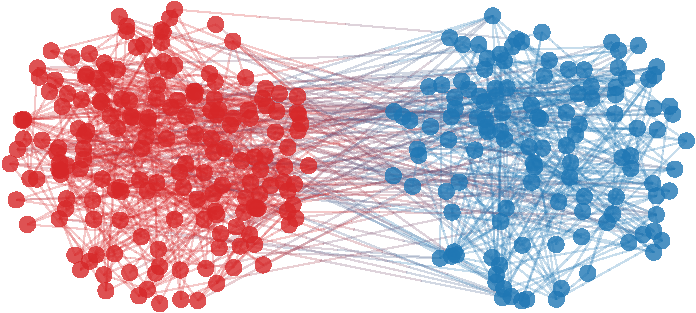
\includegraphics[width=0.7\linewidth]{Figures/2class_graph.pdf}
    \end{center}
   \caption[Visualisation of a binary classification task over a network]{An example visualisation of a binary classification task over a network, with red and blue representing the true binary labels of each node.} 
    \label{fig:binary_class_graph}
\end{figure} 

\begin{figure}[t] 
    \begin{center}
        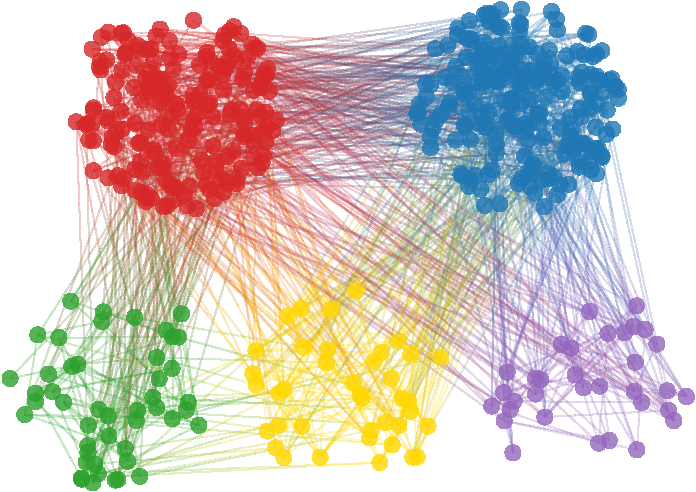
\includegraphics[width=0.7\linewidth]{Figures/multiclass_graph.pdf}
    \end{center}
   \caption[Visualisation of a multiclass classification task over a network]{An example visualisation of a multiclass classification task over a network. Here, the five distinct colours represent the true class label of each node. } 
    \label{fig:mutliclass_graph}
\end{figure} 

Within the graph signal processing community, a significant amount of research has been dedicated to the study of real-valued signals, since they are naturally well-suited to spectral analysis via the GFT and representation in terms of Gaussian random fields. By contrast, binary-valued graph signals, as well as other discrete or non-Gaussian distributions, have received notably less attention. In the machine learning community, binary graph signals have been studied in the context of semi-supervised learning, see for example \cite{Kondor2002,Zhu2003}. However, there, the graph is usually constructed by considering a distance metric in a feature space, and the focus is on maximising the utility of unlabelled data using algorithms such as label propagation (see, for example \cite{Zhang2017}). The GSP community, by contrast, focuses on statistical processes that occur over intrinsically graph-structured objects using spectral methods. While some work on binary reconstruction and regression from this perspective has occurred (see, for example \cite{Tran2020}), many of the important GSP algorithms are yet to be generalised to binary data. In this chapter, we build on the models already developed in this thesis to define several reconstruction and regression algorithms for binary graph signals. In contrast to some of the prior work discussed, these models are focused on GSP applications and are applicable to general $d$-dimensional multiway graph signals. This means they are particularly suited to multivariate applications such as hyperspectral image processing, graph time series etc.  

This chapter is structured as follows. First, in \cref{sec:lgsr}, we define a model for the reconstruction of binary graph signals on a Cartesian product graph. Here, we describe how the multiway GSR model developed in \cref{chap:nd_gsp} can be modified to produce a statistical model for the generation of binary signals in $d$ dimensions. By making use of the CGM in conjunction with the Iteratively Reweighted Least Squares (IRLS) algorithm, we demonstrate how to efficiently solve for the underlying probability tensor. Next, in \cref{sec:multiclass}, we adapt this algorithm to accommodate multiclass classification problems. This necessitates the introduction of a new class of Kronecker operator, which appears in the preconditioned coefficient matrix. Using Gerschgorin's circle theorem we are able to bound the eigenvalues of this operator and provide an upper bound for the condition number. In \cref{sec:logistic_regression}, we generalise both binary and multiclass signal reconstruction to encompass the regression models introduced in \cref{chap:kgr_rnc_2d} and extended to the multiway setting in \cref{chap:nd_gsp}. Finally, in \cref{sec:logistic_rnc_application}, we explore the behaviour of the logistic RNC model on an image segmentation task. 


\section{Logistic Graph Signal Reconstruction (L-GSR)}

\label{sec:lgsr}

In this section we define a model for the reconstruction of binary signals existing on the nodes of a $d$-dimensional Cartesian product graph, which we term Logistic Graph Signal Reconstruction (L-GSR). As before, the graph is characterised by $d$ graph Laplacians $\left\{\LL^{(i)}\right\}_{i=1}^d$, with the total Laplacian given by their Kronecker sum (see \cref{sec:dd_gsp}). The partially observed graph signal, $\Yt$, is an order-$d$ tensor of shape $(N_1, N_2, .., N_d)$, with binary-valued elements representing the two classes. This is accompanied by another binary tensor, $\St$, of the same shape which, as in previous chapters, contains the information about which elements of $\Yt$ were observed by holding ones where successful observations were made and zeros elsewhere. Where no observation was made (i.e. $\St_{\nn} = 0$), the corresponding element $\Yt_{\nn}$ is set to zero by default. The goal is to predict the value of the graph signal at elements where no observation was made using solely the topology of the graph. As such, the input data for this problem can be summarised as follows. 

\begin{equation*}
    \text{input data} = \left\{\; \Yt \in \{0, 1\}^{N_1 \times ... \times N_d}, \;\; \St \in \{0, 1\}^{N_1 \times ... \times N_d} , \;\; \left\{\LL^{(i)} \in \R^{N_i \times N_i}\right\}_{i=1}^d \; \right\}
\end{equation*}

In the following, we assume each observed element of the tensor $\Yt$ follows a Bernoulli distribution, according to some underlying latent probability tensor $\Mt$, which specifies the expected value of the outcome at each node. All other elements of $\Yt$, which were not in the set of observed elements $\mathcal{S}$, are set to zero with probability one. This can be summarised by the following statistical model. 

\begin{equation}    
    \Yt_\nn \sim  \begin{cases}
        \text{Bern}\left(\Mt_\nn \right) & \text{if} \;\; \nn \in \mathcal{S} \\
        \text{Bern}\left(0\right) & \text{otherwise}
    \end{cases}
\end{equation}


We refer to $\Mt \in [0, 1]^{N_1, ..., N_d}$ as the mean tensor. It has the same shape as $\Yt$ and elements contained within the interval $[0, 1]$ describing the probability that the corresponding entry of $\Yt$ is one. For a given mean tensor, $\Mt$, the probability of observing a binary signal $\Yt$ is given by the following expression. 

\begin{equation}
    p(\Yt \, | \, \Mt) = \prod_{\nn \in \mathcal{S}} \Mt_\nn^{\Yt_\nn}\left(1 - \Mt_\nn\right)^{1 - \Yt_\nn}
\end{equation}

As such, the log-likelihood of observing a signal $\Yt$, which is simply the natural log of this expression, is given by 

\begin{align}
   \log p(\Yt \, | \, \Mt) &= \sum_{\nn} \St_{\nn} \Big( \Yt_{\nn} \log \Mt_{\nn} + (1 - \Yt_{\nn}) \log \left(1 - \Mt_{\nn}\right) \Big) \notag \\
   &= \s^\top \big(\y \circ \log \muu + \left(\one  - \y\right) \circ \log \left(\one - \muu \right)\big) 
\end{align}

where $\s = \vecrm{\St}, \; \y = \vecrm{\Yt}$ and $\muu = \vecrm{\Mt}$. Here, the logarithm function is understood as being applied element-wise.

The goal of our L-GSR model is to estimate the value of the latent probability tensor $\Mt$ given the partially observed binary graph signal $\Yt$. The key assumption that anchors the model to the graph, and avoids underspecification, is that the probability tensor varies smoothly with respect to the topology of the Cartesian product graph. In previous chapters, when working with real-valued signals, this was achieved by setting a Gaussian prior over the latent signal $\Ft$. However, since the elements of $\Mt$ fall within the interval $[0, 1]$, we need a distribution that naturally supports this range. To achieve this, we follow the approach of standard logistic regression (see, for example, \cite{Murphy2012}), by describing the probability in terms of a logistic link function. In particular, we assume that the mean tensor, $\Mt$, is generated by applying the logistic function to a real-valued tensor graph signal $\Ft \in \R^{N_1 \times ... \times N_d}$ as follows. 

\begin{equation}
    \label{eq:logistic_link}
    \Mt(\Ft) = \frac{\one}{\one + \exp(-\Ft)} \quad \Longleftrightarrow \quad \muu(\f) = \frac{\one}{\one + \exp(-\f)}
\end{equation}

Here, the exponential and division should be interpreted as element-wise. Next, we make the assumption that $\f = \vecrm{\Ft}$ is smooth with respect to the topology of the graph by assigning it the following Gaussian prior. 

\begin{equation}
    \label{eq:f_prior_logit}
    \f  \, \sim \, \mathcal{N}\left( \zero, \, \gamma^{-1} \HH^2 \right) 
\end{equation}

As in previous chapters, the covariance matrix $\HH^2$ is the square of a graph filter operator, derived by applying a filter function $g(\cdot)$ to the product graph Laplacian. In particular, 

\begin{equation*}
    \HH = \U \D_\Gt \U^\top
\end{equation*}

where $\U$ is the Kronecker product of each of the eigenvector matrices of the individual factor graph Laplacians, and $\D_\G = \diag{\vecrm{\Gt}}$ is the diagonalised spectral scaling tensor, created by applying an isotropic or anisotropic graph filter to the corresponding eigenvalues (see \cref{sec:dd_gsp,sec:GSP_dd} for details). 

By applying this prior we encode the belief that $\Ft$ is smooth with respect to the topology of the graph, which is then applied by proxy to the mean tensor $\Mt$. In particular, $\muu$ is distributed on $[0, 1]^N$ according to a multivariate logit-normal distribution. Note that this is distinct from the multivariate logistic-normal distribution, which is produced by applying a softmax function to a random Gaussian vector to produce vectors on a simplex \citep{Atchinson1980}. \Cref{fig:logistic_gsr} gives some visual intuition for this by showing a colour-map of several smooth signals on a 2D lattice graph, along with the corresponding mean tensor $\Mt$. As visible, the qualitative smoothness properties of $\Ft$ broadly translate under the transformation of the logistic link function. That is, increasingly smooth real-valued signals correspond to increasingly smooth signals on the unit interval. 

\begin{figure}[t] 
    \begin{center}
        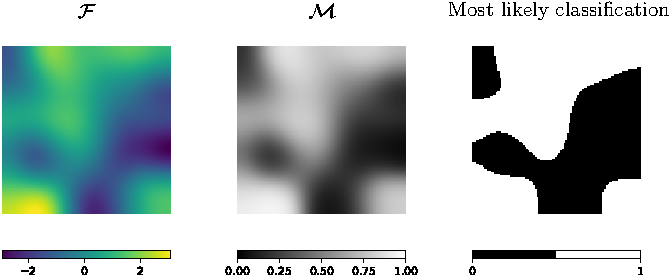
\includegraphics[width=0.9
        \linewidth]{Figures/logistic_gsr.pdf}
    \end{center}
    \caption[Visualisation of binary classification on a 2D lattice]{An example visualisation of transforming a smooth signal via the logistic link function, on a $100 \times 100$ grid of pixels ($N_1 = 100, N_2 = 100$). Left: a random smooth graph signal $\Ft$ drawn from the distribution of \cref{eq:f_prior_logit} with a diffusion filter. Middle: the value of the tensor $\Mt$ found by applying the logistic link function of \cref{eq:logistic_link}. Right: the resultant most likely classification given by $\Mt_{\nn} > 0.5$ each pixel, $\nn$. Each row shows an increasingly smooth signal by increasing the value of $\beta$ characterising the graph filter. } 
    \label{fig:logistic_gsr}
\end{figure} 

As previously stated, the goal of the L-GSR model is to find the most likely value of $\Mt$ given $\Yt$. Since we have a prior distribution over $\Ft$, we can derive an equation for its posterior distribution given $\Yt$ through the application of Bayes' rule. The Maximum A Posteriori (MAP) estimator for $\Ft$ corresponds to the value that minimises the negative log-likelihood of $\Ft \, | \, \Yt$. Given the MAP estimator for $\Ft$, we can compute the most likely mean tensor $\Mt$ by applying \cref{eq:logistic_link}. To this end, we define the objective function $\xi(\f)$, which is equal to $-\log p(\f \, | \, \y)$ up to an additive constant.
 
\begin{equation}
    \label{eq:nll_logistic}
    \xi(\f) = -\s^\top \big(\y \circ \log \muu(\f) + \left(\one  - \y\right) \circ \log \left(\one - \muu(\f) \right)\big) + \frac{\gamma}{2} \f^\top \HH^{-2} \f
\end{equation}

The goal of the next section is to find an algorithm for minimising this expression with respect to $\f$, i.e. to find the MAP estimator for $\Ft$, and subsequently compute the most likely value of the mean tensor $\Mt$. 


\subsection{Solving for the MAP estimator with the IRLS algorithm}

Unlike the normal models of the previous sections, no closed-form solution exists to minimise \cref{eq:nll_logistic}, meaning we must resort to iterative local minimisation techniques. A standard approach to solving optimisation problems of this form is to use the Iteratively Reweighted Least Squares (IRLS) algorithm. IRLS algorithms have been independently discovered several times and have been studied for over 50 years. Their main use today is found in $L^p$ norm optimisation problems such as sparse recovery (e.g. \cite{Gorodnitsky1997,Daubechies2010}) and maximum likelihood estimation within a generalized linear models \citep{Nelder1972} such as logistic regression. 

The IRLS algorithm begins with an initial estimate $\f_0$, which is then iteratively refined to reach the global minimum. It begins following update formula. 

\begin{equation}
    \label{eq:irls_update}
    \f_{k+1} = \f_{k} - \PP^{-1}(\f_k) \, \g(\f_k)
\end{equation}

where $ \g(\f) \in \R^N$ is the gradient of the optimisation objective $\xi(\f)$ with respect to the vector $\f$, and $\PP(\f) \in \R^{N \times N}$ is the Hessian, which is the matrix of second derivatives. 

\begin{equation*}
    \g_n = \frac{\partial \xi(\f)}{\partial \f_n}, \aand \PP_{nm} = \frac{\partial^2 \xi(\f)}{\partial \f_n \partial \f_m}
\end{equation*}

What differentiates the IRLS algorithm from Fisher scoring and Newton's method is that, as we will shortly demonstrate each iteration can be completed in the form of a weighted least squares solution \citep{Fan2020}. In our case, the gradient is given by 

\begin{equation}
    \g(\f) = \D_\St \big(\muu(\f) - \y\big) + \gamma \HH^{-2} \f
\end{equation}

and the Hessian is given by 

\begin{equation}
    \label{eq:logistic_gsr_P}
    \PP(\f) = \frac{\partial \g(\f)}{\partial \f} =  \D_{\muu}(\f) + \gamma \HH^{-2}
\end{equation}

where $\D_{\muu}(\f)$ is a diagonal matrix with the following definition. 

\begin{equation}
    \D_{\muu}(\f) = \text{diag}\big(\s \circ \muu(\f) \circ (\one - \muu(\f))\big)
\end{equation}

A derivation of the expressions for both gradient and the Hessian can be found in \cref{the:gradient_and_hesian}. Note that they are both a function of $\f$. 

Consider the update formula given in \cref{eq:irls_update}. Substituting in the values for $\PP$ and $\g$, and using the shorthands

\begin{equation*}
    \PP(\f_k) = \PP_k, \quad \g(\f_k) = \g_k, \quad \muu(\f_k) = \muu_k, \aand \D_{\muu}(\f_k) = \D_{\muu}^k
\end{equation*}

gives

\begin{align*}
    \f_{k+1} &= \f_k - \PP^{-1}_k \, \g_k\\
    &= \f_{k} - \PP^{-1}_k \left(\D_\St \big(\muu_k - \y\big) + \gamma \HH^{-2} \f_k\right) \\
    &= \f_k + \PP^{-1}_k \D_\St \big(\y - \muu_k\big) - \PP^{-1}_k (\gamma \HH^{-2} \f_k) \\
    &= \PP^{-1}_k \D_\St \big(\y - \muu_k \big) + \PP^{-1}_k \left(\PP_k \f_k - \gamma \HH^{-2} \f_k\right) \\
    &= \PP^{-1}_k \D_\St \big(\y - \muu_k \big) + \PP^{-1}_k \D_{\muu}^k\f_k  \\
    &= \PP^{-1}_k \left(\D_\St \big(\y - \muu_k \big) + \D_{\muu}^k\f_k \right) \\
    &= \PP^{-1}_k \tee_k
\end{align*}

where

\begin{equation}
    \tee_k = \D_\St \big(\y - \muu_k\big) + \D_{\muu}^k \f_k
\end{equation}

As visible, each iteration of the IRLS algorithm reduces to solving the linear system $\PP^{-1}_k \tee_k$, for some vector $\tee_k$. 

\subsection{Completing iterations with the CGM}

When it comes to solving the linear system $\PP^{-1}_k \tee_k$, we encounter similar challenges to those discussed in previous chapters. Specifically, the implicit dimensionality of $\PP_k$ can be substantial for tensor-valued graph signals, and the inverse-squared filter matrix $\HH^{-2}$ appearing in the definition of $\PP_k$ [see \cref{eq:logistic_gsr_P}] may suffer from ill-conditioning. Once again, these issues can be overcome by employing the SIM or CGM techniques introduced earlier in \cref{sec:SIM,sec:CGM}.


In this chapter, our focus will be on the CGM for two primary reasons. Firstly, as the dimensionality of tensor-valued binary graph signals increases, it is likely that only a small fraction of nodes will have valid observed data in most practical applications. As demonstrated in \cref{sec:GSR_convergence_implications}, the CGM exhibits superior scaling properties when the input graph signal $\Yt$ is sparsely observed. Secondly, when it comes to sampling from the posterior distribution, certain aspects of the CGM can be reused, as discussed in \cref{sec:GSR_PO}. In this chapter, we also analyse sampling-related questions in \cref{sec:lsamp} and utilise the CGM method. Hence, for the sake of simplicity, it is preferable to use the CGM in both cases instead of mixing methods.

Recall that the CGM seeks to solve a linear system by introducing the symmetric preconditioner $\PSI$, for the purpose of reducing the condition number of the coefficient matrix. In the case of logistic GSR, we can obtain an alternative expression for the update formula with a reduced condition number as follows. 

\begin{equation*}
    \f_k = \PP^{-1}_k \tee_k \quad \Longrightarrow \quad \f_k = \PSI \Q_k^{-1} \PSI^\top \tee_k
\end{equation*}

where, as in previous sections, 

\begin{equation*}
    \PSI = \U \D_\Gt
\end{equation*}

By instead solving the linear system $\Q_k^{-1} (\PSI^\top \tee_k)$ using the conjugate gradient method, and then left-multiplying the result by $\PSI$, we can obtain $\f_{k+1}$ with fewer iterative steps than solving $\PP^{-1} \tee_k$ directly. In this case, $\Q_k$ is given by the following expression. 

\begin{equation}
    \label{eq:Q_LGSR}
    \Q_k = \D_\Gt \U^\top \D_{\muu}^k \U \D_\Gt + \gamma \I_N
\end{equation}

While the condition number, $\kappa$, of $\PP$ is potentially unbounded, $\kappa(\Q)$ is guaranteed to have a maximum value of $(0.25 + \gamma) / \gamma$, as shown formally in \cref{the:L_GSR_Q_conditioning}. 

\begin{theorem}
    \label{the:L_GSR_Q_conditioning}
    
    The condition number of $\Q_k$ is bounded by a maximum value of 
    
    \begin{equation}
        \kappa(\Q_k) \leq \frac{0.25 + \gamma}{\gamma}
    \end{equation}

\end{theorem}

\begin{proof}
    As established in \cref{sec:wfl_derivation}, the worst-case convergence rate is achieved in the limit of a weak filter, where $\D_\Gt = \I_N$. In this case, the condition number of $\Q_k$ is given by 

    \begin{align*}
        \kappa(\Q_k) &= \kappa\left( \U^\top \D_{\muu}^k \U + \gamma \I_N\right) \\[0.1cm]
        &=  \kappa\left( \U^\top \left(\D_{\muu}^k + \gamma \I_N\right) \U  \right) \\[0.1cm]
        &= \kappa\left( \D_{\muu}^k + \gamma \I_N\right)
    \end{align*}

    Since $\D_{\muu}^k = \text{diag}\big(\s \circ \muu_k \circ (\one - \muu_k)\big)$, the maximum possible value along the diagonal of $\D_{\muu}^k$ will be 0.25, occurring when the corresponding element of $\muu_k$ is $1/2$. Furthermore, since $\s$ is a binary vector, the smallest possible value along the diagonal is 0. Therefore, the ratio between the largest and smallest eigenvalues of $ \D_{\muu}^k + \gamma \I_N$ must be less than or equal to $(0.25 + \gamma) / \gamma$. 
\end{proof}



\begin{algorithm}[ht]
    \begin{algorithmic}
    \vspace{0.15cm}
    \Require{Observed binary tensor $\Yt \in \{0, 1\}^{N_1 \times ... \times N_d}$}
    \vspace{0.05cm}
    \Require{Binary sensing tensor $\St \in \{0, 1\}^{N_1 \times ... \times N_d}$}
    \vspace{0.05cm}
    \Require{Cartesian product graph Laplacian $\LL \in \R^{N \times N}$}
    \vspace{0.05cm}
    \Require{Regularisation parameter $\gamma \in \R^+$}
    \vspace{0.05cm}
    \Require{Graph filter function $g(\, \cdot\, \,; \betaa)$}
    \vspace{0.25cm}
    \State{Decompose $\LL$ into $\U \LAM \U^\top$ }
    \vspace{0.15cm}
    \State{Compute $\Gt \in \R^{N_1 \times ... \times N_d}\;$ as $\;\Gt_{\nn} = g\big(\lambdaa(\nn); \, \betaa\big)$ }
    \vspace{0.15cm}
    \State{$\D_\Gt \leftarrow \diag{\vecrm{\Gt}}$}
    \vspace{0.15cm}
    \State{$\D_\St \leftarrow \diag{\vecrm{\St}}$}
    \vspace{0.15cm}
    \State{$\PSI \leftarrow \U \D_\Gt$}
    \vspace{0.15cm}
    \State{Initialise $\f \in \R^N$ randomly}
    \vspace{0.25cm}
    \While{$|\Delta \f| > \text{tol}$}
    \vspace{0.15cm}
    \State{$\muu \leftarrow \one / \big(\one + \exp(-\f)\big)$}
    \vspace{0.15cm}
    \State{$\D_{\muu} \leftarrow  \Diag{\vecrm{\s \circ \muu \circ (1 - \muu)}}$}
    \vspace{0.15cm}
    \State{$\tee \leftarrow \D_\St \big(\y - \muu\big) + \D_{\muu} \f $}
    \vspace{0.15cm}
    \State{$\Q \leftarrow  \D_\Gt \U^\top \D_{\muu} \U \D_\Gt + \gamma \I_N$}
    \vspace{0.15cm}
    \State{$\f \leftarrow \PSI \Q^{-1} \PSI^\top \tee \quad$ solve with the CGM}
    \vspace{0.15cm}
    \EndWhile
    \vspace{0.25cm}
    \State{$\muu \leftarrow \one / \big(\one + \exp(-\f)\big)$ }
    \vspace{0.15cm}
    \Ensure{$\text{reshape} \big( \muu, \, (N_1, ... N_d) \big)$}
    \end{algorithmic}
    \caption{Logistic Graph Signal Reconstruction}
    \label{al:LGSR}
\end{algorithm}

For completeness, we now give the full algorithm for logistic graph signal reconstruction in \cref{al:LGSR}. Note that, by making use of the fast Kronecker product algorithm described in \cref{sec:fast_kron_dd}, the runtime complexity of the CGM step is bounded by 

\begin{equation*}
    O\left(\frac{0.25 + \gamma}{\gamma} N \sum_{i=1}^d N_i \right)
\end{equation*}

The run time complexity of the overall algorithm of course depends on the convergence rate of the IRLS iterations. This is known to be super-linear, and approximately quadratic when a sufficiently accurate starting value is used \citep{Burden2010}. Whilst an in-depth theoretical exploration of the IRLS algorithm for this particular application is beyond the scope of this chapter, in practice, the IRLS algorithm converges very quickly, usually taking on the order of 10 steps to achieve negligible error.

\section{Multiclass Logistic Graph Signal Reconstruction}

\label{sec:multiclass}

Up to this point in the chapter, our focus has been on binary-valued graph signals, which can be used to represent two-class classification tasks over a multiway network. However, in many practical applications, the task may involve classifying each node into one of multiple distinct groups. Therefore, the objective of this section is to extend and generalise the methods we have developed thus far to encompass multiclass classification problems.

Let us first consider the task of multiclass graph signal reconstruction. Here, the goal is to classify each node, $\nn$, in a $d$-dimensional Cartesian product graph into one of $C>2$ distinct groups. To do this, we have access to the graph Laplacian $\LL \in \R^{N \times N}$, and the true class label at a subset of nodes, $\mathcal{S}$. This partially observed graph signal can be represented as an order-($d + 1$) tensor, where the last dimension contains a ``one-hot" encoding of the class label. As such, the input data can be summarised as follows. 

\begin{equation*}
    \text{input data} = \Big\{\; \Yt \in \{0, 1\}^{N_1 \times ... \times N_d \times C}, \;\; \St \in \{0, 1\}^{N_1 \times ... \times N_d} , \;\; \LL \in \R^{N \times N} \; \Big\}
\end{equation*}

As in previous sections, the tensor $\St$, of shape $(N_1 \times ... \times N_d$), indicates which nodes in the product graph have been successfully observed by holding a one in the corresponding entry, and zeros elsewhere. Note that the observed graph signal, $\Yt$, has an additional dummy dimension of length $C$ to represent the class label. Where no observation was made, the corresponding values of $\Yt_{\nn, :}$ can all be safely set to zero. 

We describe the probability that node $\nn$ has class $c$ with another tensor, $\Mt$, which, like $\Yt$, has shape $(N_1 \times ... \times N_d \times C)$. In particular, 

\begin{equation*}
    p(\text{node} \; \nn \; \text{is of class} \; c) = \Mt_{\nn, c}
\end{equation*}

Every length-$C$ fibre $\Mt_{\nn, :}$ is a probability vector, and therefore exists on a $C$-dimensional simplex with $C-1$ degrees of freedom. For a given $\Mt$, the probability of observing a signal $\Yt$ is therefore given by

\begin{equation}
    p(\Yt \, | \, \Mt) = \prod_{c, \nn \in \mathcal{S}} \Mt_{\nn, c}^{\Yt_{\nn, c}}
\end{equation}

As such, the log-likelihood of observing a signal $\Yt$ is given by 

\begin{align}
    \log p(\Yt \, | \, \Mt) &= \sum_{\nn, c} \St_{\nn} \, \Yt_{\nn, c} \log \Mt_{\nn, c} \notag \\
    &= (\s \otimes \one_C)^\top \big(\y \circ \log \muu \big)
 \end{align}
 

where, as before, $\s = \vecrm{\St}, \; \y = \vecrm{\Yt}$ and $\muu = \vecrm{\Mt}$. Furthermore, to enforce the restriction that all probabilities must sum to one, we can generate $\Mt$ by applying a softmax function to each length-$C$ fibre of a tensor $\Ft$. 

\begin{equation}
    \label{eq:softmax}
    \Mt_{\nn, c} = \frac{\exp(\Ft_{\nn, c})}{ \raisebox{-0.1cm} { $\sum_{c'=1}^C \exp(\Ft_{\nn, c'})$ }}  \quad \Longleftrightarrow \quad \muu(\f) = \frac{\exp(\f)}{ \big((\I_N \otimes \one_C) \exp(\f)\big) \otimes \one_C}
\end{equation}

Here, $\Ft$ is a real-valued tensor signal which, like $\Mt$ and $\Yt$, has shape $(N_1 \times ... \times N_d \times C)$. A graphical representation of the relation between $\Ft$, $\Mt$ and the most likely classification is shown in \cref{fig:logistic_gsr_multiclass}. The goal, then, of multiclass logistic graph signal reconstruction is to find the most likely value for the tensor $\Ft$, which allows us to make a prediction for the probability of each class by applying \cref{eq:softmax}.  

\begin{figure}[t]  
    \begin{center}
        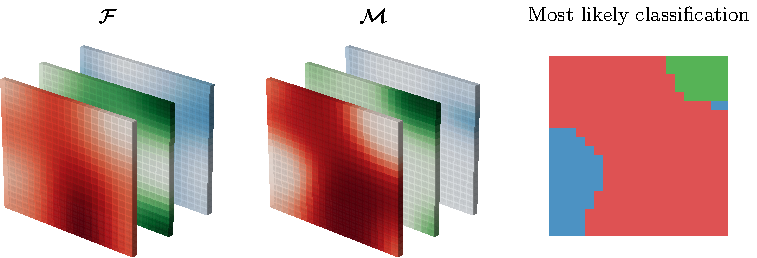
\includegraphics[width=\linewidth]{Figures/multiclass.pdf}
    \end{center}
   \caption[Visualisation of multiclass classification on a 2D lattice]{An example visualisation of multiclass classification on a $20 \times 20$ grid of pixels ($N_1 = 20, N_2 = 20, C=3$). Left: a random smooth tensor signal $\Ft$ split across three channels. Middle: the value of the tensor $\Mt$ found by applying the softmax function of \cref{eq:softmax} in the class dimension. Right: the resultant most likely classification given by the maximum probability class label for each pixel. } 
    \label{fig:logistic_gsr_multiclass}
\end{figure} 


Assuming no particular relational structure between the $C$ classes, we can encode the assumption that class probabilities should vary smoothly over the graph by assigning the following prior to $\Ft$. 

\begin{equation}
    \f \sim \Norm{\zero}{\gamma^{-1} \HH^2 \otimes \I_C}
\end{equation}

By applying Bayes' rule, we can therefore derive an expression $\xi(\f)$, representing the posterior log-likelihood of an underlying signal $\f$ given an observed signal $\y$. 

\begin{equation}
    \xi(\f) = - (\s \otimes \one_C)^\top \big(\y \circ \log \muu(\f) \big) + \frac{\gamma}{2} \f^\top \left(\HH^{-2} \otimes \I_C\right) \f
\end{equation}

Once again, we can solve for the minimising value of $\f$ using the IRLS algorithm. In this case, the gradient and Hessian are respectively given by 

\begin{equation}
    \g(\f) = \big(\D_\St \otimes \I_C\big) \big(\muu(\f) - \y\big) + \gamma \left(\HH^{-2} \otimes \I_C\right) \f
\end{equation}

and

\begin{equation}
    \PP(\f) = \RR_{\muu}(\f) + \gamma \HH^{-2} \otimes \I_C
\end{equation}

Unlike the binary model where the Hessian was the sum of a diagonal matrix $\D_{\muu}(\f)$ and $\gamma \HH^{-2}$, the matrix $\RR_{\muu}(\f)$ is no longer diagonal. In this case, $\RR_{\muu}(\f)$ is given by 

\begin{equation}
    \RR_{\muu}(\f) =  \big(\D_\St \otimes \I_C\big) \left(\Diag{\muu(\f)} - \sum_{n=1}^N \mathbf{\Delta}_{n} \otimes \m_n (\f) \m_n^\top(\f) \right)
\end{equation}

where $\m_n \in \R^C$ is the probability vector at node $n$ (i.e. the $n$-th lexicographically ordered fiber within the tensor $\Mt$), and $\mathbf{\Delta}_{n}$ is a matrix of zeros, with a single one at element $(n, n)$. Given the definition of the Kronecker product, we can see that $\RR_{\muu}(\f)$ is a block-diagonal matrix with the following structure. 

\begin{equation*}
    \RR_{\muu}(\f) = \begin{bmatrix}
        \B_1 & & & \\
        & \B_2 & & \\
        & & \ddots & \\
        & & & \B_N
    \end{bmatrix}, \quad \text{where} \quad \B_n = \s_n \Big(\diag{\m_n} - \m_n \m_n^\top\Big)
\end{equation*}

Despite no longer being diagonal, we can still leverage the block structure of this matrix to multiply $\RR_{\muu}(\f)$ onto an arbitrary vector, $\ve$, efficiently. This can be achieve as follows. 


\begin{equation}
    \label{eq:R_mu_eff}
    \RR_{\muu}(\f) \ve = (\s \otimes \one_C) \circ  \muu(\f) \circ \ve - \Big(\big((\D_\St \otimes \one_C) (\muu(\f) \circ \ve) \big) \otimes \one_C \Big) \circ \muu(\f)
\end{equation}

While a naive implementation of the product $\RR_{\muu}(\f) \ve$ would have memory time and memory complexity $O\left(C^2N^2\right)$, by following the formula given in \cref{eq:R_mu_eff}, it can instead be achieved with $O(NC)$ for both, as it would for a diagonal operator of size $(NC \times NC)$. 

Now consider the IRLS update formula. As before, we will use the following shorthands. 

\begin{equation*}
    \PP(\f_k) = \PP_k, \quad \g(\f_k) = \g_k, \quad \muu(\f_k) = \muu_k, \aand \RR_{\muu}(\f_k) = \RR_{\muu}^k
\end{equation*}

Applying the update formula gives

\begin{align*}
    \f_{k+1} &= \f_k - \PP^{-1}_k \, \g_k\\
    &= \f_{k} - \PP^{-1}_k \Big(\big(\D_\St \otimes \I_C\big) \big(\muu_k - \y\big) + \gamma \left(\HH^{-2} \otimes \I_C\right) \f_k\Big) \\
    &= \f_k + \PP^{-1}_k \big(\D_\St \otimes \I_C\big) \big(\y - \muu_k\big) - \PP^{-1}_k \Big(\gamma \left(\HH^{-2} \otimes \I_C\right) \f_k\Big) \\
    &= \PP^{-1}_k \big(\D_\St \otimes \I_C\big) \big(\y - \muu_k \big) + \PP^{-1}_k \Big(\PP_k \f_k - \gamma \left(\HH^{-2} \otimes \I_C\right) \f_k\Big) \\
    &= \PP^{-1}_k \big(\D_\St \otimes \I_C\big) \big(\y - \muu_k \big) + \PP^{-1}_k \RR_{\muu}^k\f_k  \\
    &= \PP^{-1}_k \left(\big(\D_\St \otimes \I_C\big)\big(\y - \muu_k \big) + \RR_{\muu}^k\f_k \right) \\
    &= \PP^{-1}_k \tee_k
\end{align*}

where 

\begin{equation*}
    \tee_k = \big(\D_\St \otimes \I_C\big)\big(\y - \muu_k \big) + \RR_{\muu}^k\f_k
\end{equation*}

As before, we can solve the linear system $\PP^{-1}_k \tee_k$ by introducing a symmetric preconditioner $\PSI$. The only modification is that it must be of dimension of $(NC \times NC)$, rather than $(N \times N)$. This can be achieved as follows. 

\begin{equation*}
    \PSI = \left(\U \D_\Gt\right) \otimes \I_C 
\end{equation*}

Using this, we can transform the linear system into 

\begin{equation*}
    \f_k = \PP^{-1}_k \tee_k \quad \Longrightarrow \quad \f_k = \PSI \Q_k^{-1} \PSI^\top \tee_k
\end{equation*}

where 

\begin{equation}
    \label{eq:Q_LGSR_mc}
    \Q_k = \big(\U \D_\Gt \otimes \I_C\big)^\top  \RR_{\muu}^k \big(\U \D_\Gt \otimes \I_C\big) + \gamma \I_{NC}
\end{equation}

While the condition number, $\kappa$, of $\PP$ is potentially unbounded, $\kappa(\Q)$ is guaranteed to have a maximum value of $(0.5 + \gamma) / \gamma$, as shown formally in \cref{the:L_GSR_mc_Q_conditioning}. 

\begin{theorem}
    \label{the:L_GSR_mc_Q_conditioning}
    
    The condition number of $\Q_k$ is bounded by a maximum value of 
    
    \begin{equation}
        \kappa(\Q_k) \leq \frac{0.5 + \gamma}{\gamma}
    \end{equation}

\end{theorem}

\begin{proof}
    As established in \cref{sec:wfl_derivation}, the worst-case convergence rate is achieved in the limit of a weak filter, where $\D_\Gt = \I_N$. In this case, the condition number of $\Q_k$ is given by 

    \begin{align*}
        \kappa(\Q_k) &= \kappa\left( \left(\U \otimes \I_C\right)^\top \RR_{\muu}^k \left(\U \otimes \I_C\right) + \gamma \I_{NC}\right) \\[0.1cm]
        &=  \kappa\left( \left(\U \otimes \I_C\right)^\top \left(\RR_{\muu}^k + \gamma \I_N\right) \left(\U \otimes \I_C\right)  \right) \\[0.1cm]
        &= \kappa\left( \RR_{\muu}^k + \gamma \I_N\right)
    \end{align*}

    Since $\RR_{\muu}^k$ is block-diagonal, its eigenvalues are equal to the union of the eigenvalues of each individual block. Furthermore, each block within  $\RR_{\muu}^k$ is of the form

    \begin{equation*}
        \B = s \Big(\diag{\m} - \m \m^\top\Big)
    \end{equation*}
    
    where $\m \in \R^C$ is a probability vector, and $s$ is either zero or one. For the case where $s \neq 0$, we can see that $\B$ must have at least one zero eigenvalue, with eigenvector $\one$.     

    \begin{align*}
        \B \one &= \Big(\diag{\m} - \m \m^\top\Big) \one \\
        &= \diag{\m} \one - (\m^\top \one) \m \\
        &= \m - \m = \zero
    \end{align*}

    Note, we have used the fact that $\m^\top \one = 1$, since $\m$ is a vector of probabilities. Furthermore, we can show that all eigenvalues of $\B$ must be within the interval $[0, 1/2]$, no matter the value of $\m$.  To achieve this, we can make use of the Gerschgorin circle theorem \citep{Gerschgorin1931}. This states that all eigenvalues of a square matrix must fall within at least one of the closed disks $D(a_{ii}, R_i) \subseteq \mathbb{C}$ in the complex plane. Here, $a_{ii}$ are the centres of the disks given by the diagonal elements of the matrix, and $R_i$ are the radii of the disks, given by 

    \begin{equation*}
        R_i = \sum_{j \neq i} |a_{ij}|
    \end{equation*}
    
    i.e. the sum of the absolute value of the off-diagonal elements in row $i$. Consider the structure of $\B$. 

    \begin{equation*}
        \B = \begin{bmatrix}
            m_1 - m_1^2 & -m_1 m_2 & \dots & - m_1 m_C \\
            - m_2 m_1 & m_2 - m_2^2 & \dots & -m_2 m_C \\
            \vdots & \vdots & \ddots & \vdots \\
            -m_C m_1 & -m_C m_2 & \dots &m_C- m_C^2
        \end{bmatrix}
    \end{equation*}
    
    The disk associated with row $c$ will be given by

    $$
    D\left(m_c - m_c^2, \; \sum_{c' \neq c} |-m_c m_{c'}|\right) = D\Big(m_c\,(1 - m_c), \; m_c\,(1 - m_c)\Big)
    $$
    
    In our particular scenario, the matrix $\B$ is symmetric-real, guaranteeing that its eigenvalues are real. This implies that, instead of complex regions, each of these disks represents a real interval. As such, every eigenvalue is constrained to fall within the interval $m_c\,(1 - m_c) \pm m_c\,(1 - m_c) = \big[0, \, 2 m_c\,(1 - m_c)\big]$. The maximum width of this interval occurs when $m_c = 0.5$, resulting in an interval of $[0, 0.5]$. Consequently, the largest possible eigenvalue of matrix $\B$ is 0.5.

    Finally, since $\RR_{\muu}^k$ is composed of blocks $\B_n$, this means the largest possible eigenvalue of $\RR_{\muu}^k$ is 0.5, and the smallest is zero. Therefore

    \begin{equation*}
        \kappa\left( \RR_{\muu}^k + \gamma \I_N\right) = \frac{0.5 + \gamma}{\gamma}
    \end{equation*}

\end{proof}

For completeness, we now give the full algorithm for logistic graph signal reconstruction in \cref{al:LGSR}. Note that, by making use of the fast Kronecker product algorithm described in \cref{sec:fast_kron_dd}, the runtime complexity of the CGM step is bounded by 

\begin{equation*}
    O\left(\frac{0.5 + \gamma}{\gamma} NC \Big(C + \sum_{i=1}^d N_i \Big)\right)
\end{equation*}

\begin{algorithm}[ht]
    \begin{algorithmic}
    \vspace{0.15cm}
    \Require{Observed binary tensor $\Yt \in \{0, 1\}^{N_1 \times ... \times N_d \times C}$}
    \vspace{0.05cm}
    \Require{Binary sensing tensor $\St \in \{0, 1\}^{N_1 \times ... \times N_d}$}
    \vspace{0.05cm}
    \Require{Cartesian product graph Laplacian $\LL \in \R^{N \times N}$}
    \vspace{0.05cm}
    \Require{Regularisation parameter $\gamma \in \R^+$}
    \vspace{0.05cm}
    \Require{Graph filter function $g(\, \cdot\, \,; \betaa)$}
    \vspace{0.25cm}
    \State{Decompose $\LL$ into $\U \LAM \U^\top$ }
    \vspace{0.15cm}
    \State{Compute $\Gt \in \R^{N_1 \times ... \times N_d}$ as $\Gt_{\nn} = g\big(\lambdaa(\nn); \, \betaa\big)$ }
    \vspace{0.15cm}
    \State{$\D_\Gt \leftarrow \diag{\vecrm{\Gt}}$}
    \vspace{0.15cm}
    \State{$\D_\St \leftarrow \diag{\vecrm{\St}}$}
    \vspace{0.15cm}
    \State{$\PSI \leftarrow \U \D_\Gt \otimes \I_C$}
    \vspace{0.15cm}
    \State{Initialise $\f \in \R^{NC}$ randomly}
    \vspace{0.25cm}
    \While{$|\Delta \f| > \text{tol}$}
    \vspace{0.15cm}
    \State{$\muu \leftarrow \exp(\f) / \big((\I_N \otimes \one_C) \exp(\f)\big) \otimes \one_C$}
    \vspace{0.15cm}
    \State{$\M \leftarrow \text{reshape}\big(\muu, (N, C)\big)$}
    \vspace{0.15cm}
    \State{$\RR_{\muu} \leftarrow  \big(\D_\St \otimes \I_C\big) \left(\Diag{\muu} - \sum_{n=1}^N \mathbf{\Delta}_{n} \otimes \m_n \m_n^\top \right)\quad$ ($\m_n$ is the $n$-th row of $\M$)}
    \vspace{0.15cm}
    \State{$\tee \leftarrow \big(\D_\St \otimes \I_C\big)\big(\y - \muu \big) + \RR_{\muu}\f$}
    \vspace{0.15cm}
    \State{$\Q \leftarrow  \big(\U \D_\Gt \otimes \I_C\big)^\top  \RR_{\muu} \big(\U \D_\Gt \otimes \I_C\big) + \gamma \I_{NC}$}
    \vspace{0.15cm}
    \State{$\f \leftarrow \PSI \Q^{-1} \PSI^\top \tee \quad$ (solve with the CGM)}
    \vspace{0.15cm}
    \EndWhile
    \vspace{0.25cm}
    \State{$\muu \leftarrow \exp(\f) / \big((\I_N \otimes \one_C) \exp(\f)\big) \otimes \one_C$}
    \vspace{0.15cm}
    \Ensure{$\text{reshape}\big(\muu, (N_1, ..., N_d, C)\big)$}
    \end{algorithmic}
    \caption{Multiclass Logistic Graph Signal Reconstruction}
    \label{al:LGSR_mc}
\end{algorithm}

\section{Logistic Graph Signal Regression} 

\label{sec:logistic_regression}

So far in this chapter we have developed binary and multiclass multiway graph signal reconstruction algorithms, where no additional data exists to help predict the value of the graph signal at the unlabelled nodes. In this section, we consider several scenarios in which explanatory variables are available and consider models for utilising this information to estimate the underlying class label probabilities.

\subsection{Logistic Kernel Graph Regression (L-KGR)}

\label{sec:lkgr}

The first models we consider are binary and multiclass Logistic Kernel Graph Regression (L-KGR), applicable to general tensor-valued inputs. As in previous sections, the KGR model can be understood as a relatively simple extension of graph signal reconstruction. First let us consider the case of binary classification. Here, we have a sequence of $T$ partially observed binary tensor graph signals, each of shape $(N_1, ..., N_d)$. These are stacked into a single tensor $\Yt$ of shape $(T, N_1, ..., N_d)$ and accompanied by the binary sensing tensor, $\St$, indicating which values were observed and which were missing. In addition, at each time instant, we have a length-$M$ vector of explanatory variables $\x_t$, which can be stacked together into a matrix $\X$ with shape $(T, M)$. The goal is to utilise the explanatory variables, plus the topology of the underlying graph, to estimate the class probability at each node, at each time instant. The relevant input data can therefore be described as follows. 


\begin{multline*}
    \text{input data} = \Bigg\{\;\X \in \R^{T \times M}, \;\; \Yt \in \{0, 1\}^{T \times N_1 \times ... \times N_d}, \;\; \\ 
    \St \in \{0, 1\}^{T \times N_1 \times ... \times N_d} , \;\; \left\{\LL^{(i)} \in \R^{N_i \times N_i}\right\}_{i=1}^d \; \Bigg\}
\end{multline*}

Following the same pattern as the KGR algorithms of previous sections (see \cref{sec:KGR_and_GSR} for details and further explanation), we can easily derive a model for the prediction of the class probability given the features $\X$ by making a small modification to the L-GSR algorithm of \cref{sec:lgsr}. Once again, we assume each element of $\Yt$ is distributed according to a Bernoulli distribution, with a mean given by the tensor $\Mt$. Furthermore, we assume $\Mt$ is smooth with respect to the topology of the graph, \textit{and} varies smoothly with with respect to the feature space. This is encoded via a tensor $\Ft$, which is again related to $\Mt$ via the logistic link function of \cref{eq:logistic_link}. We apply these assumptions by setting the following prior distribution for $\f = \vecrm{\Ft}$. 

\begin{equation}
    \f \sim \Norm{\zero}{\gamma \K \otimes \HH^2}
\end{equation}


As before, $\K$ is the $T \times T$ kernel matrix created by applying a symmetric function, such as the Gaussian kernel, $\kappa(\cdot, \cdot)$ to pairs of feature vectors such that $\K_{ij} = \kappa(\x_i, \x_j)$. Next, we compute the eigendecompostion of $\K$ as $\K = \V \LAM_K \V^\top$. Finally, we define the transformed variables $\bar{\U}$ and $\bar{\Gt}$ as follows. 

\begin{equation}
    \bar{\U} \in \R^{NT \times NT} = \V \otimes \U, \aand \bar{\Gt}_{t, \nn} \in \R^{T \times N_1 \times ... \times N_d} = g(\lambdaa(\nn), \betaa) \sqrt{\lambda_t^{(K)}}
\end{equation}

where $\lambda_t^{(K)}$ is the $t$-th eigenvalue of $\K$. The L-KGR algorithm then follows by modifying \cref{al:LGSR} by substituting every instance of $\U$ for $\bar{\U}$ and every instance of $\Gt$ for $\bar{\Gt}$. 

The same principles can be used to generate a multiclass logistic kernel graph regression algorithm. In this case, the input data is a sequence of $T $ partially observed multiway graph signals where each observed node has been classified into one of $C > 2$ classes. This can be represented by the binary tensor $\Yt$ with shape $(T \times N_1 \times ... \times N_d \times C)$, where an extra dimension has been added containing a one-hot encoding of the class label. Where no data was recorded, the full length-$C$ fibre at time $t$ and node $\nn$ can be set to zero. As such, the data is described as follows. 

\begin{multline*}
    \text{input data} = \Bigg\{\;\X \in \R^{T \times M}, \;\; \Yt \in \{0, 1\}^{T \times N_1 \times ... \times N_d \times C}, \;\; \\ 
    \St \in \{0, 1\}^{T \times N_1 \times ... \times N_d} , \;\; \left\{\LL^{(i)} \in \R^{N_i \times N_i}\right\}_{i=1}^d \; \Bigg\}
\end{multline*}

Just as in \cref{sec:multiclass}, we describe the probability that node $(t, \nn)$ has class probability $c$ with the tensor $\Mt$, which has the same shape as $\Yt$. As before, $\Mt$ is described by a real-valued tensor, $\Ft$, according to the multivariate softmax function given in \cref{eq:softmax}, only here it is modified slightly such that 

\begin{equation}
    \label{eq:softmax2}
    \Mt_{t, \nn, c} = \frac{\exp(\Ft_{t, \nn, c})}{ \raisebox{-0.1cm} { $\sum_{c'=1}^C \exp(\Ft_{t, \nn, c'})$ }}  \quad \Longleftrightarrow \quad \muu(\f) = \frac{\exp(\f)}{ \big((\I_{NT} \otimes \one_C) \exp(\f)\big) \otimes \one_C}
\end{equation}

We then place a prior over the signal $\f = \vecrm{\Ft} \in \R^{TNC}$ of

\begin{equation}
    \f \sim \Norm{\zero}{\gamma \K \otimes \HH^2 \otimes \I_C}
\end{equation}

This encodes the belief that each of the $c$ class probabilities should vary smoothly (and independently) with respect to the topology of the graph and the feature space. once again, the full procedure for outputting the tensor $\Mt$ can be achieved by running \cref{al:LGSR_mc} after substituting the variables $\U \rightarrow \bar{\U}$ and $\G \rightarrow \bar{\G}$. 


\subsection{Logistic Regression with Network Cohesion (L-RNC) }

\label{sec:lrnc}

In this section we present models for binary and multiclass Logistic Regression with Network Cohesion (L-RNC). In this scenario, we encounter a partially observed tensor graph signal $\Yt$, with shape $(N_1 \times ... \times N_d)$, where a subset of the nodes have been labelled with the true class. In addition, each node in the Cartesian product graph has an associated length-$M$ vector of explanatory variables, collected into the tensor $\Xt$ with shape $(N_1 \times ... \times N_d \times M)$. The goal is to predict the class probabilities at each node $\nn$. Once again, we also have a binary tensor $\St$ describing which nodes have been observed. As such, the data for the binary L-RNC algorithm can be summarised as follows. 

\begin{multline*}
    \text{input data} = \Bigg\{\;\Xt \in \R^{N_1 \times ... \times N_d \times M}, \;\; \Yt \in \{0, 1\}^{N_1 \times ... \times N_d}, \;\; \\ 
    \St \in \{0, 1\}^{N_1 \times ... \times N_d} , \;\; \left\{\LL^{(i)} \in \R^{N_i \times N_i}\right\}_{i=1}^d \; \Bigg\}
\end{multline*}

As with the GSR model, we suppose that each observed element of $\Yt$ is a Bernoulli random variable, with the probability of success given by the tensor $\Mt \in [0, 1]^{N_1 \times ... \times N_d}$. However, unlike the GSR model, we assume that $\Mt$ is generated according to the following expression. 

\begin{equation}
    \muu(\cc, \w) = \frac{\one}{\one + \exp\big(-(\cc + \X \w) \big)}
\end{equation}

Here, $\cc = \vecrm{\Ct}$ is a real-valued vector form of a tensor $\Ct$, which is assumed to vary smoothly with respect to the topology of the multiway graph, $\X$ is the tensor of explanatory variables reshaped into a matrix of dimensions $(N \times M)$ (see \cref{eq:X_RNC_dd}), and $\w \in \R^M$ is the length-$M$ vector coefficients specifying the contribution of each of the columns of $\X$. As in previous sections on RNC, we can stack $\cc$ and $\w$ into a single parameter vector $\thetaa$, such that 

\begin{equation}
    \muu(\thetaa) = \frac{\one}{\one + \exp\big(-\big[\I_N \;\; \X \big] \thetaa \big)}
\end{equation}

Furthermore, we can place a prior over $\thetaa$ that encodes the belief that $\Ct$ should be smooth with respect to the graph, as well as preventing overfitting of $\w$ with an L2 penalty. 

\begin{equation}
    \thetaa \sim \Norm{\zero}{\begin{bmatrix}\gamma^{-1} \HH^2 & \zero \\
    \zero & \lambda^{-1} \I_M \end{bmatrix}}
\end{equation}

As such, the MAP estimator for $\thetaa$ is given by the minimiser of the following expression. 

\begin{equation}
    \label{eq:nll_logistic_rnc}
    \widetilde{\xi}(\thetaa) = -\s^\top \big(\y \circ \log \muu(\thetaa) + \left(\one  - \y\right) \circ \log \left(\one - \muu(\thetaa) \right)\big) + \frac{1}{2} \thetaa^\top \begin{bmatrix}\gamma^{1} \HH^{-2} & \zero \\
        \zero & \lambda^{1} \I_M \end{bmatrix}\thetaa
\end{equation}

Proceeding in the same way as L-GSR, we must compute both the gradient, $\widetilde{\g}(\thetaa)$, and the Hessian, $\widetilde{\PP}(\thetaa)$, of this expression with respect to $\thetaa$. These are given by 

\begin{equation}
    \widetilde{\g}(\thetaa) \in \R^{N + M} = \begin{bmatrix}
        \D_\St \\ \X^\top \D_\St
    \end{bmatrix} \big(\muu(\thetaa) - \y\big) + \begin{bmatrix}
        \gamma^{-1} \HH^2 & \zero \\
    \zero & \lambda^{-1} \I_M
    \end{bmatrix} \thetaa
\end{equation}

and 

\begin{equation}
    \widetilde{\PP}(\thetaa)  \in \R^{(N + M) \times (N + M)} = \begin{bmatrix}
        \D_{\muu}(\thetaa) + \gamma \HH^{-2} & \D_{\muu}(\thetaa) \X \\ 
        \X^\top \D_{\muu}(\thetaa)  & \X^\top \D_{\muu}(\thetaa) \X + \lambda \I_M
    \end{bmatrix}
\end{equation}

where, as with L-GSR, 

\begin{equation}
    \D_{\muu}(\thetaa) \in \R^{N \times N} = \text{diag}\big(\s \circ \muu(\thetaa) \circ (\one - \muu(\thetaa))\big)
\end{equation}

Then, using the shorthands 

\begin{equation*}
    \widetilde{\PP}(\thetaa_k) = \widetilde{\PP}_k, \quad \widetilde{\g}(\thetaa_k) = \widetilde{\g}_k, \quad \muu(\thetaa_k) = \muu_k, \aand \D_{\muu}(\thetaa_k) = \D_{\muu}^k
\end{equation*}

IRLS update formula is then given by 

\begin{align*}
    \thetaa_{k + 1} &= \thetaa_k - \widetilde{\PP}^{-1}_k \, \widetilde{\g}_k \\
    &= \thetaa_k - \widetilde{\PP}^{-1}_k \left( \begin{bmatrix}
        \D_\St \\ \X^\top \D_\St
    \end{bmatrix} \big(\muu_k - \y\big) + \begin{bmatrix}
        \gamma^{-1} \HH^2 & \zero \\
    \zero & \lambda^{-1} \I_M
    \end{bmatrix} \thetaa_k \right)\\
    &= \thetaa_k + \widetilde{\PP}^{-1}_k  \begin{bmatrix}
        \D_\St \\ \X^\top \D_\St
    \end{bmatrix} \big(\y - \muu_k\big) - \widetilde{\PP}^{-1}_k  \begin{bmatrix}
        \gamma^{-1} \HH^2 & \zero \\
    \zero & \lambda^{-1} \I_M
    \end{bmatrix} \thetaa_k \\
    &=  \widetilde{\PP}^{-1}_k  \begin{bmatrix}
        \D_\St \\ \X^\top \D_\St
    \end{bmatrix} \big(\y - \muu_k\big) + \widetilde{\PP}^{-1}_k  \left(\widetilde{\PP}_k \thetaa_k - \begin{bmatrix}
        \gamma^{-1} \HH^2 & \zero \\
    \zero & \lambda^{-1} \I_M
    \end{bmatrix} \thetaa_k \right)\\
    &=  \widetilde{\PP}^{-1}_k  \begin{bmatrix}
        \D_\St \\ \X^\top \D_\St
    \end{bmatrix} \big(\y - \muu_k\big) + \widetilde{\PP}^{-1}_k  \begin{bmatrix}
        \D_{\muu}^k & \D_{\muu}^k \X \\ 
        \X^\top \D_{\muu}^k  & \X^\top \D_{\muu}^k \X
    \end{bmatrix} \thetaa_k \\
    &=  \widetilde{\PP}^{-1}_k  \begin{bmatrix}
        \D_\St \\ \X^\top \D_\St
    \end{bmatrix} \left(\y - \muu_k + \D_{\muu}^k \big[\I_N \;\; \X \big] \thetaa_k \right) \\
    &= \widetilde{\PP}_k^{-1} \widetilde{\tee}_k 
\end{align*}

where 

\begin{equation}
    \widetilde{\tee}_k = \begin{bmatrix}
        \D_\St \\ \X^\top \D_\St
    \end{bmatrix} \left(\y - \muu_k + \D_{\muu}^k \big[\I_N \;\; \X \big] \thetaa_k \right)
\end{equation}

Note that, in the derivation above, we have used the fact that $\D_\St \D_{\muu}^k = \D_{\muu}^k \D_\St = \D_{\muu}^k$. 

As before, the linear system $\widetilde{\PP}_k^{-1} \widetilde{\tee}_k $ cannot easily be solved in this form due to ill-conditioning. To overcome this issue, we can again use the symmetrically preconditioned CGM. In particular, we can transform the system into 

\begin{equation*}
    \thetaa_k = \widetilde{\PP}^{-1}_k \widetilde{\tee}_k \quad \Longrightarrow \quad \thetaa_k = \widetilde{\PSI}_k \widetilde{\Q}_k^{-1} \widetilde{\PSI}_k^\top \widetilde{\tee}_k
\end{equation*}

In order to define $\widetilde{\PSI}_k$ and $\widetilde{\Q}_k$, first we must compute the eigendecomposition of $\X^\top \D_{\muu}^k \X$. 

\begin{equation}
    \X^\top \D_{\muu}^k \X = \U_M^k \LAM_M^k (\U_M^k)^\top 
\end{equation}

Next, we define the matrix $\D_M^k$ as follows. 

\begin{equation}
    \D_M^k = \left(\LAM_M^k + \lambda \I_M\right)^{-1/2}
\end{equation}

Then, the operators $\widetilde{\PSI}_k$ and $\widetilde{\Q}_k$ are defined as follows. 

\begin{equation}
    \widetilde{\PSI}_k = \begin{bmatrix}
        \U \D_\Gt & \zero \\
        \zero & \U_M^k \D_M^k
    \end{bmatrix}
\end{equation}

and 

\begin{equation}
    \widetilde{\Q}_k = 
       \begin{bmatrix}
        \D_\Gt \U^\top \D_{\muu}^k \U \D_\Gt + \gamma \I_{NT}  &  \D_\Gt \U^\top \D_{\muu}^k \X \U_M^k \D_M^k \\[0.1cm] 
        \D_M^k \left(\U_M^k\right)^\top \X^\top \D_{\muu}^k \U \D_\Gt & \I_M
        \end{bmatrix}
\end{equation}

Note that, in contrast to L-GSR, the preconditioning matrix $\widetilde{\PSI}_k$ is changing on each iteration of the IRLS algorithm. For clarity, we now present the complete L-RNC algorithm in \cref{al:LRNC}. 


\begin{algorithm}[ht]
    \begin{algorithmic}
    \vspace{0.15cm}
    \Require{Explanatory variables $\Xt \in \R^{N_1 \times ... \times N_d \times M}$}
    \vspace{0.05cm}
    \Require{Observed binary tensor $\Yt \in \{0, 1\}^{N_1 \times ... \times N_d}$}
    \vspace{0.05cm}
    \Require{Binary sensing tensor $\St \in \{0, 1\}^{N_1 \times ... \times N_d}$}
    \vspace{0.05cm}
    \Require{Cartesian product graph Laplacians $\left\{\LL^{(i)} \in \R^{N_i \times N_i}\right\}_{i=1}^d$}
    \vspace{0.05cm}
    \Require{Regularisation parameter $\gamma \in \R^+$}
    \vspace{0.05cm}
    \Require{Graph filter function $g(\, \cdot\, \,; \betaa)$}
    \vspace{0.05cm}
    \Require{Regularisation parameter $\lambda \in \R^+$}
    \vspace{0.25cm}
    \State{$\X \leftarrow \text{reshape}\big(\Xt, (N, M)\big)$ }
    \vspace{0.15cm}
    \State{$\y \leftarrow \vecrm{\Yt}$ }
    \vspace{0.15cm}
    \State{$\s \leftarrow \vecrm{\St}$ }
    \vspace{0.15cm}
    \State{Decompose each $\LL^{(i)}$ into $\U^{(i)} \LAM^{(i)} \left(\U^{(i)}\right)^\top$ }
    \vspace{0.15cm}
    \State{$\U \leftarrow \bigotimes \U^{(i)}$ }
    \vspace{0.15cm}
    \State{Compute $\Gt \in \R^{N_1 \times ... \times N_d}\;$ as $\;\Gt_{\nn} = g\big(\lambdaa(\nn); \, \betaa\big) \quad$ (see \cref{eq:Gn_dd2,eq:lam_of_n})}
    \vspace{0.15cm}
    \State{$\D_\Gt \leftarrow \diag{\vecrm{\Gt}}$}
    \vspace{0.15cm}
    \State{$\D_\St \leftarrow \diag{\s}$}
    \vspace{0.15cm}
    \State{Initialise $\thetaa \in \R^{N+M}$ randomly}
    \vspace{0.25cm}
    \While{$|\Delta \thetaa| > \text{tol}$}
    \vspace{0.15cm}
    \State{$\muu \leftarrow \one / \one + \exp\big(-\big[\I_N \;\; \X \big] \thetaa \big)$}
    \vspace{0.15cm}
    \State{$\D_{\muu} \leftarrow  \Diag{\s \circ \muu \circ (1 - \muu)}$}
    \vspace{0.15cm}
    \State{Decompose $\X^\top \D_{\muu} \X$ into $\U_M \LAM_M \U_M^\top$ }
    \vspace{0.15cm}
    \State{$\D_M \leftarrow  \left(\LAM_M + \lambda \I_M\right)^{-1/2}$}
    \vspace{0.15cm}
    \State{$\PSI \leftarrow  \begin{bmatrix}
        \U \D_\Gt & \zero \\
        \zero & \U_M \D_M
    \end{bmatrix}$}
    \vspace{0.15cm}
    \State{$\tee \leftarrow \begin{bmatrix}
        \D_\St \\ \X^\top \D_\St
    \end{bmatrix} \left(\y - \muu + \D_{\muu} \big[\I_N \;\; \X \big] \thetaa \right)$}
    \vspace{0.15cm}
    \State{$\Q \leftarrow \begin{bmatrix}
        \D_\Gt \U^\top \D_{\muu} \U \D_\Gt + \gamma \I_{NT}  &  \D_\Gt \U^\top \D_{\muu} \X \U_M \D_M \\[0.1cm] 
        \D_M \U_M^\top \X^\top \D_{\muu} \U \D_\Gt & \I_M
        \end{bmatrix}$}
    \vspace{0.15cm}
    \State{$\thetaa \leftarrow \PSI \Q^{-1} \PSI^\top \tee \quad$ solve with the CGM}
    \vspace{0.15cm}
    \EndWhile
    \vspace{0.25cm}
    \State{$\muu \leftarrow \one / \one + \exp\big(-\big[\I_N \;\; \X \big] \thetaa \big)$ }
    \vspace{0.15cm}
    \Ensure{$\text{reshape} \big( \muu, \, (N_1, ..., N_d) \big)$}
    \end{algorithmic}
    \caption{Logistic Regression with Network Cohesion}
    \label{al:LRNC}
\end{algorithm}

\subsection{Multiclass Logistic Regression with Network Cohesion}

In this section we take the multiclass L-GSR model developed in \cref{sec:multiclass} and adapt it for the purpose of RNC. The data available in this scenario is very similar to that of binary L-RNC, except the observed tensor input signal $\Yt$ now has an extra final dimension of length $C$ which contains a one hot encoding of the class label. As such, the data can be described as follows. 

\begin{multline*}
    \text{input data} = \Bigg\{\;\Xt \in \R^{N_1 \times ... \times N_d \times M}, \;\; \Yt \in \{0, 1\}^{N_1 \times ... \times N_d \times C}, \;\; \\ 
    \St \in \{0, 1\}^{N_1 \times ... \times N_d} , \;\; \left\{\LL^{(i)} \in \R^{N_i \times N_i}\right\}_{i=1}^d \; \Bigg\}
\end{multline*}

Just as in \cref{sec:multiclass}, we describe the probability that node $\nn$ is of class $C$ with the tensor $\Mt$, which has the same shape as $\Yt$. Each fibre $\Mt_{\nn, :}$ is a probability vector existing on a $C$-dimensional simplex with $C - 1$ degrees of freedom. As before, the log-likelihood of observing a signal $\Yt$ is given by 

\begin{align}
   \log p(\Yt \, | \, \Mt) &= \sum_{\nn, c} \St_{\nn} \, \Yt_{\nn, c} \log \Mt_{\nn, c} \notag \\
   &= (\s \otimes \one_C)^\top \big(\y \circ \log \muu \big)
\end{align}

Furthermore, we assume that $\Mt$ is generated by applying a softmax function to each length-$C$ fibre of another tensor $\Ft$ according to

\begin{equation}
    \Mt_{\nn, c} = \frac{\exp(\Ft_{\nn, c})}{ \raisebox{-0.1cm} { $\sum_{c'=1}^C \exp(\Ft_{\nn, c'})$ }}  \quad \Longleftrightarrow \quad \muu(\f) = \frac{\exp(\f)}{ \big((\I_N \otimes \one_C) \exp(\f)\big) \otimes \one_C}
\end{equation}

where 

\begin{equation}
    \Ft = \Ct + \tenrm{\left(\X \otimes \I_C \right) \w} \quad \Longleftrightarrow \quad \f = \cc + \left(\X \otimes \I_C \right) \w
\end{equation}
    
Here, $\Ct$ is a tensor with shape $(N_1, ..., N_d, C)$ and $\w$ is a coefficient vector of length $MC$. The effect of this assumption is that each slice of the tensor $\Ft$, $\Ft_{:, c}$ is the sum of a tensor $\Ct_{:, c}$ and an independent linear combination of slices of the tensor $\Xt_{:, m}$. We can stack $\cc$ and $\w$ into a single vector $\thetaa$ as follows. 

\begin{equation}
    \thetaa \in \R^{NC + MC} = \begin{bmatrix}
        \cc \\ \w
    \end{bmatrix}
\end{equation}

Then, $\f$ can be rewritten as 

\begin{equation}
    \f = \begin{bmatrix}
        \I_{NC} & \X \otimes \I_C 
    \end{bmatrix} \thetaa
\end{equation}

As such, we can rewrite the formula for $\muu$ in terms of $\thetaa$. 

\begin{equation}
 \muu(\thetaa) = \frac{\exp\left(\big[\I_N \;\; \X \otimes \I_C \big] \thetaa\right)}{ \Big( \big(\I_N \otimes \one_C\big) \exp\big(\big[\I_N \;\; \X \otimes \I_C\big] \thetaa\big)\Big) \otimes \one_C}
\end{equation}

Next, we place the following prior over $\thetaa$. 

\begin{equation}
    \thetaa \sim \Norm{\zero}{\begin{bmatrix}\gamma^{-1} \HH^2 \otimes \I_C & \zero \\
    \zero & \lambda^{-1} \I_{MC} \end{bmatrix}}
\end{equation}


This leads to the following negative log-likelihood. 

\begin{equation}
    \xi(\thetaa) = - (\s \otimes \one_C)^\top \big(\y \circ \log \muu(\thetaa) \big) + \frac{1}{2} \thetaa^\top \begin{bmatrix}\gamma \HH^{-2} \otimes \I_C & \zero \\
        \zero & \lambda \I_{MC} \end{bmatrix} \thetaa
\end{equation}

The gradient is given by 

\begin{equation}
    \g(\thetaa) \in \R^{NC + MC} = \begin{bmatrix}
        \D_\St \otimes \I_C \\ \left(\X^\top \D_\St\right) \otimes \I_C
    \end{bmatrix} \big(\muu(\thetaa) - \y\big) + \begin{bmatrix}
        \gamma \HH^{-2} \otimes \I_C & \zero \\
    \zero & \lambda \I_{MC}
    \end{bmatrix} \thetaa
\end{equation}

The Hessian $\widetilde{\PP}(\thetaa)$ with shape $(NC + MC) \times (NC + MC)$  is given by


\begin{equation}
    \widetilde{\PP}(\thetaa) = \begin{bmatrix}
        \RR_{\muu}(\thetaa) + \gamma \HH^{-2} \otimes \I_C & \RR_{\muu}(\thetaa) (\X \otimes \I_C) \\ 
        (\X^\top \otimes \I_C) \RR_{\muu}(\thetaa)  & (\X^\top \otimes \I_C) \RR_{\muu}(\thetaa) (\X \otimes \I_C) + \lambda \I_{MC}
    \end{bmatrix}
\end{equation}

where 

\begin{equation}
    \RR_{\muu}(\thetaa) =  \big(\D_\St \otimes \I_C\big) \left(\Diag{\muu(\thetaa)} - \sum_{n=1}^N \mathbf{\Delta}_{n} \otimes \m_n (\thetaa) \m_n^\top(\thetaa) \right)
\end{equation}

The IRLS algorithm then proceeds as. 

\begin{align*}
    \thetaa_{k+1} &= \thetaa_k - \PP^{-1}_k \, \g_k\\
    &= \thetaa_k - \PP^{-1}_k \left(\begin{bmatrix}
        \D_\St \otimes \I_C \\ \left(\X^\top \D_\St\right) \otimes \I_C
    \end{bmatrix} \big(\muu_k - \y\big) + \begin{bmatrix}
        \gamma \HH^{-2} \otimes \I_C & \zero \\
    \zero & \lambda \I_{MC}
    \end{bmatrix} \thetaa_k \right) \\
    &= \thetaa_k + \PP^{-1}_k \begin{bmatrix}
        \D_\St \otimes \I_C \\ \left(\X^\top \D_\St\right) \otimes \I_C
    \end{bmatrix} \big(\y - \muu_k\big) - \PP^{-1}_k  \begin{bmatrix}
        \gamma \HH^{-2} \otimes \I_C & \zero \\
    \zero & \lambda \I_{MC}
    \end{bmatrix} \thetaa_k \\
    &= \PP^{-1}_k \begin{bmatrix}
        \D_\St \otimes \I_C \\ \left(\X^\top \D_\St\right) \otimes \I_C
    \end{bmatrix} \big(\y - \muu_k\big) + \PP^{-1}_k \Big(\PP_k \thetaa_k - \begin{bmatrix}
        \gamma \HH^{-2} \otimes \I_C & \zero \\
    \zero & \lambda \I_{MC}
    \end{bmatrix} \thetaa_k\Big) \\
    &= \PP^{-1}_k \begin{bmatrix}
        \D_\St \otimes \I_C \\ \left(\X^\top \D_\St\right) \otimes \I_C
    \end{bmatrix} \big(\y - \muu_k\big) + \PP^{-1}_k \begin{bmatrix}
        \RR_{\muu}^k & \RR_{\muu}^k (\X \otimes \I_C) \\ 
        (\X^\top \otimes \I_C) \RR_{\muu}^k  & (\X^\top \otimes \I_C) \RR_{\muu}^k (\X \otimes \I_C) 
    \end{bmatrix} \thetaa_k \\
    &= \PP^{-1}_k  \begin{bmatrix}
        \D_\St \otimes \I_C \\ \left(\X^\top \D_\St\right) \otimes \I_C
    \end{bmatrix} \left( \y - \muu_k + \RR_{\muu}^k  \big[\I_N \;\; \X \otimes \I_C\big] \thetaa_k \right) \\
    &= \PP^{-1}_k \tee_k
\end{align*}

where 

\begin{equation}
    \tee_k = \begin{bmatrix}
        \D_\St \otimes \I_C \\ \left(\X^\top \D_\St\right) \otimes \I_C
    \end{bmatrix} \left( \y - \muu_k + \RR_{\muu}^k  \big[\I_N \;\; \X \otimes \I_C\big] \thetaa_k \right)
\end{equation}

As before, the linear system $\widetilde{\PP}_k^{-1} \widetilde{\tee}_k $ cannot easily be solved in this form due to ill-conditioning. To overcome this issue, we can again use the symmetrically preconditioned CGM. In particular, we can transform the system into 

\begin{equation*}
    \thetaa_k = \widetilde{\PP}^{-1}_k \widetilde{\tee}_k \quad \Longrightarrow \quad \thetaa_k = \widetilde{\PSI}_k \widetilde{\Q}_k^{-1} \widetilde{\PSI}_k^\top \widetilde{\tee}_k
\end{equation*}

In order to define $\widetilde{\PSI}_k$ and $\widetilde{\Q}_k$, first we must compute the eigendecomposition of $\X^\top \RR_{\muu}^k \X$. 

\begin{equation}
    \X^\top \RR_{\muu}^k \X = \U_M^k \LAM_M^k (\U_M^k)^\top 
\end{equation}

Next, we define the matrix $\D_M^k$ as follows. 

\begin{equation}
    \D_M^k = \left(\LAM_M^k + \lambda \I_M\right)^{-1/2}
\end{equation}

Then, the operators $\widetilde{\PSI}_k$ and $\widetilde{\Q}_k$ are defined as follows. 

\begin{equation}
    \widetilde{\PSI}_k = \begin{bmatrix}
        \U \D_\Gt & \zero \\
        \zero & \U_M^k \D_M^k
    \end{bmatrix}
\end{equation}

and 

\begin{equation}
    \widetilde{\Q}_k = 
       \begin{bmatrix}
        \D_\Gt \U^\top \RR_{\muu}^k \U \D_\Gt + \gamma \I_{NT}  &  \D_\Gt \U^\top \RR_{\muu}^k \X \U_M^k \D_M^k \\[0.1cm] 
        \D_M^k \left(\U_M^k\right)^\top \X^\top \RR_{\muu}^k \U \D_\Gt & \I_M
        \end{bmatrix}
\end{equation}

\begin{algorithm}[ht]
    \begin{algorithmic}
    \vspace{0.15cm}
    \Require{Explanatory variables $\Xt \in \R^{N_1 \times ... \times N_d \times M}$}
    \vspace{0.05cm}
    \Require{Observed binary tensor $\Yt \in \{0, 1\}^{N_1 \times ... \times N_d \times C}$}
    \vspace{0.05cm}
    \Require{Binary sensing tensor $\St \in \{0, 1\}^{N_1 \times ... \times N_d}$}
    \vspace{0.05cm}
    \Require{Cartesian product graph Laplacians $\left\{\LL^{(i)} \in \R^{N_i \times N_i}\right\}_{i=1}^d$}
    \vspace{0.05cm}
    \Require{Graph regularisation parameter $\gamma \in \R^+$}
    \vspace{0.05cm}
    \Require{Graph filter function $g(\, \cdot\, \,; \betaa)$}
    \vspace{0.05cm}
    \Require{Feautre regularisation parameter $\lambda \in \R^+$}
    \vspace{0.25cm}
    \State{$\X \leftarrow \text{reshape}\big(\Xt, (N, M)\big)$ }
    \vspace{0.15cm}
    \State{$\y \leftarrow \vecrm{\Yt}$ }
    \vspace{0.15cm}
    \State{$\s \leftarrow \vecrm{\St}$ }
    \vspace{0.15cm}
    \State{Decompose each $\LL^{(i)}$ into $\U^{(i)} \LAM^{(i)} \left(\U^{(i)}\right)^\top$ }
    \vspace{0.15cm}
    \State{$\U \leftarrow \bigotimes \U^{(i)}$ }
    \vspace{0.15cm}
    \State{Compute $\Gt \in \R^{N_1 \times ... \times N_d}\;$ as $\;\Gt_{\nn} = g\big(\lambdaa(\nn); \, \betaa\big) \quad$ (see \cref{eq:Gn_dd2,eq:lam_of_n})}
    \vspace{0.15cm}
    \State{$\D_\Gt \leftarrow \diag{\vecrm{\Gt}}$}
    \vspace{0.15cm}
    \State{$\D_\St \leftarrow \diag{\s}$}
    \vspace{0.15cm}
    \State{Initialise $\thetaa \in \R^{N+M}$ randomly}
    \vspace{0.25cm}
    \While{$|\Delta \thetaa| > \text{tol}$}
    \vspace{0.15cm}
    \State{$\muu \leftarrow \exp\left(\big[\I_N \;\; \X \otimes \I_C \big] \thetaa\right)/ \Big( \big(\I_N \otimes \one_C\big) \exp\big(\big[\I_N \;\; \X \otimes \I_C\big] \thetaa\big)\Big) \otimes \one_C $}
    \vspace{0.15cm}
    \State{$\M \leftarrow \text{reshape}\big(\muu, (N, C)\big)$}
    \vspace{0.15cm}
    \State{$\RR_{\muu} \leftarrow  \big(\D_\St \otimes \I_C\big) \left(\Diag{\muu} - \sum_{n=1}^N \mathbf{\Delta}_{n} \otimes \m_n \m_n^\top \right)\quad$ ($\m_n$ is the $n$-th row of $\M$)}
    \vspace{0.15cm}
    \State{Decompose $\X^\top  \RR_{\muu} \X$ into $\U_M \LAM_M \U_M^\top$ }
    \vspace{0.15cm}
    \State{$\D_M \leftarrow  \left(\LAM_M + \lambda \I_M\right)^{-1/2}$}
    \vspace{0.15cm}
    \State{$\PSI \leftarrow  \begin{bmatrix}
        \U \D_\Gt & \zero \\
        \zero & \U_M \D_M
    \end{bmatrix}$}
    \vspace{0.15cm}
    \State{$\tee \leftarrow \begin{bmatrix}
        \D_\St \\ \X^\top \D_\St
    \end{bmatrix} \left(\y - \muu +  \RR_{\muu} \big[\I_N \;\; \X \big] \thetaa \right)$}
    \vspace{0.15cm}
    \State{$\Q \leftarrow \begin{bmatrix}
        \D_\Gt \U^\top \RR_{\muu} \U \D_\Gt + \gamma \I_{NT}  &  \D_\Gt \U^\top \RR_{\muu} \X \U_M \D_M \\[0.1cm] 
        \D_M \U_M^\top \X^\top \RR_{\muu} \U \D_\Gt & \I_M
        \end{bmatrix}$}
    \vspace{0.15cm}
    \State{$\thetaa \leftarrow \PSI \Q^{-1} \PSI^\top \tee \quad$ solve with the CGM}
    \vspace{0.15cm}
    \EndWhile
    \vspace{0.25cm}
    \State{$\muu \leftarrow \exp\left(\big[\I_N \;\; \X \otimes \I_C \big] \thetaa\right)/ \Big( \big(\I_N \otimes \one_C\big) \exp\big(\big[\I_N \;\; \X \otimes \I_C\big] \thetaa\big)\Big) \otimes \one_C $}    
    \vspace{0.15cm}
    \Ensure{$\text{reshape} \big( \muu, \, (N_1, ..., N_d) \big)$}
    \end{algorithmic}
    \caption{Multiclass Logistic Regression with Network Cohesion}
    \label{al:LRNC_mc}
\end{algorithm}


\section{Image segmentation with L-RNC}

\label{sec:logistic_rnc_application}

\cite{Li2012}

% \section{Approximate Sampling via the Laplace Approximation}

% \label{sec:lsamp}



\chapter{Conclusions} % Main chapter title

\label{chap:conclusions} % Change X to a consecutive number; for referencing this chapter elsewhere, use \ref{ChapterX}

\lhead{Chapter 7. \emph{Conclusions}} % Change X to a consecutive number; this is for the header on each page - perhaps a shortened title


\section{Main Section 1}








\addtocontents{toc}{\vspace{2em}} % Add a gap in contents

\appendix % Cue to tell LaTeX that the following 'chapters' are Appendices

% Include the appendices of the thesis as separate files from the Appendices folder
% Uncomment the lines as you write the Appendices

% Appendix A

\chapter{Proofs} % Main appendix title

\label{AppendixA} % For referencing this appendix elsewhere, use \ref{AppendixA}

\lhead{Appendix A. \emph{Proofs}} % This is for the header on each page - perhaps a shortened title

\begin{theorem}

    \label{the:F_posterior}
    The posterior distribution for $\F$ is given by 

    \begin{equation}
            \vecc{\F} \, | \, \Y \sim \mathcal{N} \big(\SIG \, \vecc{\Y}, \; \SIG \big)
        \end{equation}
        
        \noindent where 
        
        \begin{equation}
            \SIG = \Big(\diag{\vecc{\Ss}} + \gamma  \HH^{-2}\Big)^{-1}
        \end{equation}

\end{theorem}

\begin{proof}
    Consider the matrix $\Ss_{\epsilon}$ defined in the following manner. 
    
    \begin{equation}
        (\Ss_{\epsilon})_{nt} = \begin{cases}
            1 & \text{if} \;\; (n, t) \in \mathcal{S} \\
            \epsilon & \text{otherwise}
        \end{cases}
    \end{equation}

    We can use this definition to rewrite equation \ref{eq:Y_given_F} for the probability distribution of $\Y | \F$.

    \begin{equation}
        \vecc{\Y} \, | \, \F \, \sim \, \lim_{\epsilon \rightarrow 0} \, \Bigg[ \, \mathcal{N}\Big(\vecc{\Ss_{\epsilon} \circ \F}, \; \diag{\vecc{\Ss_{\epsilon}}}\Big) \, \Bigg]
    \end{equation}

    In this way, the negative log-likelihood of an observation $\Y | \F$ is given by 

    \begin{equation}
        \label{eq:log_prob_1}
        - \log \pi(\Y | \F) = \lim_{\epsilon \rightarrow 0} \, \Bigg[  \frac{1}{2} \vecc{\Ss_{\epsilon} \circ \F - \Y}^\top \diag{\vecc{\Ss_{\epsilon}}}^{-1} \vecc{\Ss_{\epsilon} \circ \F - \Y}\, \Bigg]
    \end{equation}

    up to an additive constant which does not depend on $\F$. Note that, since $\Y = \Ss_{\epsilon}  \circ \Y$, we can rewrite $\vecc{\Ss_{\epsilon} \circ \F - \Y}$ as 

    \begin{align}
        \vecc{\Ss_{\epsilon} \circ \F - \Y} &= \vecc{\Ss_{\epsilon} \circ  (\F - \Y)}  \notag \\
        &= \diag{\vecc{\Ss_{\epsilon}}} \vecc{\F - \Y}
    \end{align}

    Therefore, equation \ref{eq:log_prob_1} can be rewritten as 

    \begin{align}
        - \log \pi(\Y | \F) &= \lim_{\epsilon \rightarrow 0} \, \Bigg[  \frac{1}{2} \vecc{\F - \Y}^\top \diag{\vecc{\Ss_{\epsilon}}} \, \vecc{\F - \Y}\, \Bigg] \notag \\[0.2cm]
        &= \frac{1}{2} \vecc{\F - \Y}^\top \diag{\vecc{\Ss}} \, \vecc{\F - \Y}
    \end{align}

    Now consider the full log-posterior. Using Bayes rule, this can be written as 

    \begin{multline}
        -\log \pi\big(\vecc{\F} \, | \, \Y \big) = \frac{1}{2} \vecc{\F - \Y}^\top \diag{\vecc{\Ss}} \, \vecc{\F - \Y} \; + \\ \frac{\gamma}{2} \vecc{\F }^\top\HH^{-2} \, \vecc{\F}
    \end{multline}

    Up to an additive constant not dependent $\F$, this can be written as 

    \begin{equation}
        -\log \pi\big(\vecc{\F} \, | \, \Y \big) = \frac{1}{2} \Big( \vecc{\F}^\top \big( \diag{\vecc{\Ss}} + \gamma \HH^{-2}\big) \vecc{\F} - 2 \, \vecc{\Y}^\top \F \Big)
    \end{equation}

    Using the conjugacy of the normal distribution, by direct inspection we can conclude that the posterior covariance is given by 

    \begin{equation}
        \SIG = \Big( \diag{\vecc{\Ss}} + \gamma \HH^{-2} \Big)^{-1}
    \end{equation}

    and that the posterior mean is given by $\SIG \, \vecc{\Y}$. 

\end{proof}


\begin{theorem}
    \label{the:Z_transform_bayes}

    \normalfont
    
    Consider the random matrix $\Z$ which is related to the random matrix $\F$ as follows. 
    
    $$
    \F = \U_N \, (\G \circ \Z) \, \U_T^\top 
    $$
    
    \noindent or, equivalently,
    
    $$
    \vecc{\F} = \big(\U_T \otimes \U_N\big) \D_\G \, \vecc{\Z}
    $$
    
    Then the posterior mean for $\Z | \Y$ is given by 
    
    $$
    \text{E}\big[\Z | \Y \big] = \big( \C + \gamma \I_T \otimes \I_N \big)^{-1}\vecc{\G \circ (\U_N^\top \Y \U_T)} 
    $$
    
    \noindent where
    
    $$
    \C = \D_{\G} \, \big(\U_T^\top \otimes \U_N^\top \big)\, \D_{\Ss} \, \big(\U_T \otimes \U_N \big) \,\D_{\G}
    $$
    
    (Here we have abbreviated $\diag{\vecc{\G}}$ and $\diag{\vecc{\Ss}}$ as $\D_{\G}$ and $\D_{\Ss}$ respectively.)
    
    \end{theorem}
    
    
    \begin{proof}
    
    The conditional distribution of $\Y | \Z$ is obtained by substituting in the definition of $\F$ in terms of $\Z$ into the original conditional likelihood expression.  
    
    $$
    \vecc{\Y} \, | \, \Z \sim \mathcal{N}\Big(\vecc{\Ss \circ \big(\U_N \, (\G \circ \Z) \, \U_T^\top\big)}, \; \D_{\Ss}\Big)
    $$
    
    Similarly, since the prior specified for $\F$ is $\mathcal{N}\big(\mathbf{0}, \, \gamma^{-1} \HH^2\big)$, this implies that the prior over $\Z$ is simply
    
    $$
    \vecc{\Z} \sim \mathcal{N}\big(\mathbf{0}, \, \gamma^{-1} \I_{NT} \big) 
    $$
    
    To see this, consider the following
    
    
    \begin{align*}
    \text{Cov}\big[\vecc{\F}\big] &=  \text{Cov}\big[\big(\U_T \otimes \U_N\big) \D_\G \, \vecc{\Z}\big]  \\[0.2cm]
    &= \big(\U_T \otimes \U_N\big) \D_\G \text{Cov}\big[\vecc{\Z}\big] \D_\G \big(\U_T^\top \otimes \U_N^\top \big) 
    \end{align*}
    
    \vspace{0.2cm}
    
    If $\vecc{\Z}$ has covariance $\gamma^{-1} \I$, then $\vecc{\F}$ has covariance given by 
    
    \begin{align*}
    \text{Cov}\big[\vecc{\F}\big] &= \gamma^{-1} \big(\U_T \otimes \U_N\big) \D_\G^2 \big(\U_T^\top \otimes \U_N^\top \big) \\
    &= \gamma^{-1} \HH^{2}
    \end{align*}
    
    \noindent by the definition of $\HH$.\\
    
    Now consider the transformed posterior 
    
    \begin{align*}
    -\log p(\Z | \Y) &= -\log p(\Y | \Z) -\log p(\Z) \\
    &= \frac{1}{2} \vecc{\U_N \, (\G \circ \Z) \, \U_T^\top - \Y}^\top \times \\ &  \D_\Ss \,  \vecc{\U_N \, (\G \circ \Z) \, \U_T^\top- \Y} \\ & \quad\quad   +\frac{\gamma}{2} \, \vecc{\Z}^\top \vecc{\Z}
    \end{align*}
    
    Up to an additive constant, this is equal to 
    
    \begin{align*}
    -\log p(\Z | \Y) &= \frac{1}{2} \vecc{\Z}^\top \Big(\C + \gamma \I_{NT}\Big) \vecc{\Z} \\ & \quad - \vecc{\U_N \, (\G \circ \Z) \, \U_T}^\top \,  \vecc{\Y} \\[0.2cm]
    &= \frac{1}{2} \vecc{\Z}^\top \Big(\C + \gamma \I_{NT}\Big) \vecc{\Z} \\ & \quad - \vecc{\Z}^\top\vecc{\G \circ (\U_N^\top \Y \U_T)}
    \end{align*}
    
    By inspection, again, we can see that the posterior mean for $\Z$ is 
    
    $$
    \big( \C + \gamma \I_T \otimes \I_N \big)^{-1}\vecc{\G \circ (\U_N^\top \Y \U_T)} 
    $$
    
    
    
    \end{proof}
    

\begin{theorem}
    \label{the:SIM_convergence}
    The number of steps required to reach a given level of precision for matrix splitting methods follows 

    \begin{equation}
        n_{\text{SIM}} \propto -\frac{1}{\log \rho(\M^{-1}\N)}
    \end{equation}

    where the coefficient matrix is split as $\M - \N$. 
\end{theorem}

\begin{proof}
    In the SIM, we have that 

\begin{equation}
    \label{eq:SIM_F_true}
\M \vecc{\F} =  \N \vecc{\F} + \vecc{\Y}
\end{equation}

where $\vecc{\F}$ represents the true solution to the linear system. This leads directly to an update equation given by

\begin{equation}
    \label{eq:SIM_F_update}
\M \vecc{\F_k} = \N \vecc{\F_{k-1}} + \vecc{\Y}
\end{equation}

Subtracting \cref{eq:SIM_F_true} from \cref{eq:SIM_F_update} gives

\begin{align}
    \M \vecc{\F_k} - \M \vecc{\F} &= \N \vecc{\F_{k-1}} - \N \vecc{\F}  \notag \\
    \vecc{\E_k} &= \M^{-1} \N \vecc{\E_{k-1}} \notag \\
     &= \big( \M^{-1} \N \big)^{k} \vecc{\E_{0}}
\end{align}

where we denote the error at the $k$-th iteration as $\vecc{\E_k} = \vecc{\F_k} - \vecc{\F}$. From this it is clear to see that convergence will be achieved so long as the spectral radius $\rho(\M^{-1}\N)$ is less than one. If this condition holds then,

\begin{equation}
    \lim_{k \rightarrow \infty} \vecc{\E_{k}} = \lim_{k \rightarrow \infty} (\M^{-1} \N)^{k} \, \vecc{\E_0} = \mathbf{0} .
\end{equation}

In general, the number of iterations required to achieve some specified reduction in the magnitude of the error is proportional to one over the logarithm of the spectral radius
\end{proof}

\begin{theorem}
    \label{the:gamma_deriv_negative}
    The values of $n_{\text{SIM}}$ and $n_{\text{CGM}}$ always increase when $\gamma$, within its valid range, decreases in both the strong a weak filter limits. 
\end{theorem}

\begin{proof}
    Consider each of the following expressions.

    \begin{equation*}
        n_{\text{SIM}}(\gamma ; \; \beta \rightarrow 0) =  \frac{1}{\log(1 + \gamma)}
     \end{equation*}

     \begin{equation*}
        n_{\text{CGM}}(\gamma ; \; \beta \rightarrow 0) = \sqrt{\frac{1}{\gamma} + 1}
     \end{equation*}

    \begin{equation*}
        n_{\text{SIM}}(\gamma, m; \; \beta \rightarrow \infty) =  \frac{1}{\log(1 + \gamma) - \log m}
    \end{equation*}

    \begin{equation*}
        n_{\text{CGM}}(\gamma, m; \; \beta \rightarrow \infty) = \sqrt{\frac{1 - m + \gamma}{\gamma}}
    \end{equation*}

In order to prove the theorem, we must show that the partial derivative of each expression with respect to $\gamma$ is strictly negative over the domain $0 \leq \gamma \leq \infty$. Let us compute this for each expression in turn. 

\begin{equation*}
    \frac{\partial \,  n_{\text{SIM}}(\gamma ; \; \beta \rightarrow 0)}{\partial \, \gamma} = - \frac{1}{(1 + \gamma)\log^2(1 + \gamma)}
\end{equation*}

\begin{equation*}
    \frac{\partial \,  n_{\text{CGM}}(\gamma ; \; \beta \rightarrow 0)}{\partial \, \gamma}  = - \frac{1}{2 \gamma^2 \sqrt{\frac{1}{\gamma} + 1}}
\end{equation*}

\begin{equation*}
    \frac{\partial \,  n_{\text{SIM}}(\gamma, m ; \; \beta \rightarrow \infty)}{\partial \, \gamma}  =  - \frac{1}{(1 + \gamma)\big(\log(1 + \gamma) - \log(m) \big)^2}
\end{equation*}

\begin{equation*}
    \frac{\partial \,  n_{\text{CGM}}(\gamma, m ; \; \beta \rightarrow \infty)}{\partial \, \gamma}  = - \frac{1 - m}{2 \gamma^2 \sqrt{\frac{1 - m + \gamma}{\gamma}}}
\end{equation*}

In each of these expressions we have a fraction for which both the numerator and denominator can easily be shown to be strictly positive over the valid ranges of $\gamma$ and $m$. Each expression also includes a negative sign in front. As such, every expression is strictly negative. 

\end{proof}

\begin{theorem}
    \label{the:m_deriv}
    In the limit of a strong filter, for any fixed value of $\gamma$, the number of iterations for convergence will always increase as the proportion of missing data $m$ increases for the SIM, whereas it the number will always decrease for the CGM.  
\end{theorem}

\begin{proof}
    To prove this theorem it suffices to show that the partial derivative of $n_\text{SIM}$ with respect to $m$ is always positive, whereas the partial derivative of $n_\text{CGM}$ with respect to $m$ is always negative. They are respectively given by 

    \begin{equation*}
        \frac{\partial \,  n_{\text{SIM}}(\gamma, m ; \; \beta \rightarrow \infty)}{\partial \, m}  =  \frac{1}{m\big(\log(1 + \gamma) - \log(m) \big)^2}
    \end{equation*}
    
    \begin{equation*}
        \frac{\partial \,  n_{\text{CGM}}(\gamma, m ; \; \beta \rightarrow \infty)}{\partial \, m}  = - \frac{1}{2 \gamma \sqrt{\frac{1 - m + \gamma}{\gamma}}}
    \end{equation*}

    Since $\gamma$ is strictly positive and $m$ must be in the range $0 \leq m \leq 1$, clearly the first expression is always positive whereas the second is always negative. 
    
\end{proof}

\begin{theorem}
    \label{the:RNC_post}
    In the RNC model, the posterior distribution over the combined parameter vector $\thetaa$ is given by 

    \begin{equation}
        \thetaa \, | \, \Y \sim \mathcal{N}\left(\widetilde{\PP}^{-1} \begin{bmatrix} \vecc{\Y} \\ \X^\top \vecc{\Y} \end{bmatrix}, \, \widetilde{\PP}^{-1}\right)
    \end{equation}

    where 

    \begin{equation}
        \widetilde{\PP} \in \R^{(NT + M) \times (NT + M)}= 
        \begin{bmatrix}
         \D_\Ss + \gamma \HH^{-2} & \D_\Ss  \X \\
         \X^\top \D_\Ss & \X^\top \D_\Ss \X + \lambda \I_M   
        \end{bmatrix}
    \end{equation}

\end{theorem}

\begin{proof}

    The distribution of $\Y$ given $\thetaa$ is given in \cref{eq:Y_given_theta_rnc}. This can also be written as

    \begin{equation}
        \vecc{\Y} \, | \, \thetaa \sim \mathcal{N}\left(  \big[ \D_\Ss \;\; \D_\Ss \X \big]\thetaa  , \; \D_\Ss \right)
    \end{equation}

    The prior for $\thetaa$ is given in equation \cref{eq:theta_prior}. Therefore, using Bayes rule, we can write 

    \begin{align*}
        -2\log \pi(\thetaa | \Y) &\propto \Big(\vecc{\Y} - \big[ \D_\Ss \;\; \D_\Ss \X \big] \thetaa \Big)^\top \D_\Ss^{-1} \Big(\vecc{\Y} - \big[ \D_\Ss \;\; \D_\Ss \X \big] \thetaa \Big) \\[0.2cm]
        & + \thetaa^\top  \begin{bmatrix}
            \gamma^{-1} \HH^{2} & \mathbf{0}\\
            \mathbf{0} & \lambda^{-1} \I_M   
           \end{bmatrix} ^{-1} \thetaa
    \end{align*}

    Using the same trick as in \cref{the:F_posterior}, where we parametrise $\Ss$ as $\Ss = \lim_{\epsilon \rightarrow 0} \Ss_{\epsilon}$. Given this, we can rewrite the above expression as 

    \begin{align*}
        -2\log \pi(\thetaa | \Y) &\propto \Big(\vecc{\Y} - \big[ \I_{NT} \;\; \X \big] \thetaa \Big)^\top \D_\Ss\Big(\vecc{\Y} - \big[ \I_{NT} \;\; \X \big] \thetaa \Big) \\[0.2cm]
        & + \thetaa^\top  \begin{bmatrix}
            \gamma \HH^{-2} & \mathbf{0}\\
            \mathbf{0} & \lambda \I_M   
           \end{bmatrix} \thetaa
    \end{align*}

    Collecting like terms, and dropping a constant not dependent on $\thetaa$, this can be written as 

    \begin{align*}
        -2\log \pi(\thetaa | \Y) &\propto -2 \thetaa^\top \begin{bmatrix} \vecc{\Y} \\ \X^\top \vecc{\Y} \end{bmatrix} + \thetaa^\top \begin{bmatrix}
            \D_\Ss + \gamma \HH^{-2} & \D_\Ss  \X \\
            \X^\top \D_\Ss & \X^\top \D_\Ss \X + \lambda \I_M   
           \end{bmatrix} \thetaa
    \end{align*}

    Using the conjugacy of the normal distribution, we can conclude by direct inspection that the posterior covariance matrix is given by $\widetilde{\PP}^{-1}$, and the posterior mean is given by 

    $$
    \widetilde{\PP}^{-1} \begin{bmatrix} \vecc{\Y} \\ \X^\top \vecc{\Y} \end{bmatrix}
    $$

    where 

    $$
    \widetilde{\PP} = \begin{bmatrix}
        \D_\Ss + \gamma \HH^{-2} & \D_\Ss  \X \\
        \X^\top \D_\Ss & \X^\top \D_\Ss \X + \lambda \I_M   
       \end{bmatrix}
    $$

\end{proof}


\begin{theorem}
    \label{the:efficient_H_diag}

    This diagonal of the matrices $\HH$ and $\HH^2$ can be efficiently calculated. 
\end{theorem}

\begin{proof}
    Hi 
\end{proof}
%\input{Appendices/AppendixB}
%\input{Appendices/AppendixC}


\addtocontents{toc}{\vspace{2em}} % Add a gap in contents

\label{Bibliography}

\lhead{\emph{Bibliography}} % Change the page header to say "Bibliography"

\bibliographystyle{apalike} % Use the "apalike" BibTeX style for formatting the Bibliography

\bibliography{Bibliography} % The references (bibliography) information are stored in the file named "Bibliography.bib"


\end{document}